\documentclass[a4paper, twoside, 12pt]{article}
\usepackage[subpreambles=true]{standalone}
\usepackage[utf8]{inputenc}
\usepackage[T1]{fontenc}
\usepackage{graphicx}
\usepackage{longtable}
\usepackage{xstring}
\usepackage{etoolbox}
\usepackage{relsize}
\usepackage{caption}
%%% making 'figure label' bold and upper case
% \DeclareCaptionLabelFormat{bsc}{\textbf{\textsc{#1}\ #2}}
% \captionsetup[figure]{labelformat=bsc}
\captionsetup{labelfont=bf,tableposition=top}
\DeclareCaptionType{codeenv}[Code Listing][List of Code Listings] 


% this is only for development purposes
\usepackage[colorinlistoftodos,color=green!20,textsize=small,prependcaption={},textwidth=4cm]{todonotes}
\presetkeys{todonotes}{inline,backgroundcolor=yellow}{}

% set margins for double-sided printing
\usepackage[left=2.5cm, right=2.5cm, top=2.5cm, bottom=2.5cm, bindingoffset=1.5cm, head=15pt]{geometry} 
\usepackage{setspace}
\onehalfspacing
% set headers
\usepackage{fancyhdr}
\pagestyle{fancy}
\renewcommand{\sectionmark}[1]{\markright{\thesection~- ~#1}}
% \renewcommand{\chaptermark}[1]{\markboth{\chaptername~\thechapter~-~ #1}{}}
\fancyhead{}
\fancyfoot{}
% \fancyhead[LE]{\footnotesize\scshape\leftmark}
\fancyhead[RO]{\footnotesize\scshape\rightmark}
\fancyhead[LE]{\footnotesize\scshape\leftmark}
% \fancyhead[RE,LO]{\thesisauthor}
\fancyfoot[C]{\thepage}
\renewcommand{\headrulewidth}{0.4pt}
\renewcommand{\footrulewidth}{0pt}


\usepackage{minted}
\AtBeginEnvironment{minted}{\singlespacing%
    \fontsize{7}{7}\selectfont}

\usepackage{listings}
\lstset{language = Python}
% \newenvironment{codeenv}{\captionsetup{type=listing}}{}


\usepackage[backend=biber,style=alphabetic,natbib=true,citestyle=authoryear]{biblatex}
\addbibresource{thesis.bib}
\pagenumbering{gobble}

\usepackage{svg}

\usepackage{hyperref}
\hypersetup{colorlinks=true,linkcolor=blue,filecolor=magenta,urlcolor=cyan}
\urlstyle{same}
\usepackage[capitalise]{cleveref}
\crefname{codelisting}{Code Listing}{Code Listings}

\usepackage{tikz,pgf}


%%%%%%%%%%%%%%%%%%%%%%%%%%%%%%%%%%%%%%%%%%%%%%%%%%%%%%%%%%%%%
%THESIS Parameters 
%%%%%%%%%%%%%%%%%%%%%%%%%%%%%%%%%%%%%%%%%%%%%%%%%%%%%%%%%%%%%

\title{Tools and workflows for complex collaborative neuroscientific projects - from Experiment to Analysis}

\newcommand{\thesisdate}{January 01, 2020}
\newcommand{\thesisauthor}{Julia Sprenger}
\newcommand{\thesistype}{PhD Thesis}
% \newcommand{\supervisor}{Prof. Dr. Sonja Grün}
% \newcommand{\cosupervisor}{???}


%%%%%%%%%%%%%%%%%%%%%%%%%%%%%%%%%%%%%%%%%%%%%%%%%%%%%%%%%%%%%
%custom commands
\newcommand{\code}[1]{\texttt{{#1}}}
\newcommand{\software}[1]{\texttt{{#1}}}


%%%%%%%%%%%%%%%%%%%%%%%%%%%%%%%%%%%%%%%%%%%%%%%%%%%%%%%%%%%%%
%DOCUMENT
%%%%%%%%%%%%%%%%%%%%%%%%%%%%%%%%%%%%%%%%%%%%%%%%%%%%%%%%%%%%%


\begin{document}

%%%%%%%%%%%%%%%%%%%%%%%%%%%%%%%%%%%%%%%%%%%%%%%%%%%%%%%%%%%%%
%TITLE PAGE (Pre-defined, just change parameters above)
%%%%%%%%%%%%%%%%%%%%%%%%%%%%%%%%%%%%%%%%%%%%%%%%%%%%%%%%%%%%%
%%%%%%%%%%%%%%%%%%%%%%%%%%%%%%%%%%%%%%%%%%%%%%%%%%%%%%%%%%%%%
%TITLE PAGE
%%%%%%%%%%%%%%%%%%%%%%%%%%%%%%%%%%%%%%%%%%%%%%%%%%%%%%%%%%%%%
\makeatletter
\begin{titlepage}
    \begin{center}
        \vspace*{1cm}
        \Large
        \textbf{\@title}\\
        \vspace{3.5cm}
        \large\texfbf
        Der Fakultät Mathematik, Informatik und Naturwissenschaften\\
        der RWTH Aachen University vorgelegte Dissertation\\
        zur Erlangung des akademischen Grades einer Doktorin der Naturwissenschaften\\
        \vspace{2cm}
        von\\
        \large{\textbf{\thesisauthor{}}}\\
        \authordegree\\
        \vspace{0.5cm}
        aus \authorbirthplace\\
        \vspace{2cm}
        \@date
    \end{center}
\end{titlepage}
\makeatother


%%%%%%%%%%%%%%%%%%%%%%%%%%%%%%%%%%%%%%%%%%%%%%%%%%%%%%%%%%%%%
%SOOA
%%%%%%%%%%%%%%%%%%%%%%%%%%%%%%%%%%%%%%%%%%%%%%%%%%%%%%%%%%%%%
%\clearpage
\thispagestyle{empty}
\section*{Eidesstattliche Versicherung}
\label{sec:SOOA}

\vspace{2.5cm}

% Statement of original authorship - Needs to be in German
% see also here: https://www.wiso.uni-koeln.de/sites/fakultaet/dokumente/PA/formulare/eidesstattliche_erklaerung.pdf


% RWTH Version
Ich versichere hiermit an Eides Statt, dass ich die vorliegende Arbeit selbstständig  und  ohne  unzulässige  fremde  Hilfe (insbes.  akademisches  Ghostwriting) erbracht habe. Ich habe keine anderen als die angegebenen Quellen und Hilfsmittel benutzt. Für den Fall, dass die Arbeit zusätzlich auf einem Datenträger eingereicht wird, erkläre ich, dass die schriftliche und die elektronische Form vollständig übereinstimmen. Die Arbeit hat in gleicher oder ähnlicher Form noch keiner Prüfungsbehörde vorgelegen.

% Cologne Version
Hiermit versichere ich an Eides statt, dass ich die vorliegende Arbeit selbstständig und ohne die Benutzung anderer als der angegebenen Hilfsmittel angefertigt habe. Alle Stellen, die wörtlich oder sinngemäß aus veröffentlichten und nicht veröffentlichten Schriften entnommen wurden, sind als solche kenntlich gemacht. Die Arbeit ist in gleicher oder ähnlicher Form oder auszugsweise im Rahmen einer anderen Prüfung noch nicht vorgelegt worden. Ich versichere, dass die eingereichte elektronische Fassung der eingereichten Druckfassung vollständig entspricht.

\vspace{1cm}

\noindent
Die Strafbarkeit einer falschen eidesstattlichen Versicherung ist mir bekannt, namentlich die Strafandrohung gemäß § 156 StGB bis zu drei Jahren Freiheitsstrafe oder Geldstrafe bei vorsätzlicher Begehung der Tat bzw. gemäß § 161 Abs. 1 StGB bis zu einem Jahr Freiheitsstrafe oder Geldstrafe bei fahrlässiger Begehung.

\vspace{3cm}
\noindent
\textbf{\thesisauthor{}} 

\vspace{0.5cm}
\noindent
Köln, den xx.xx.20xx

\clearpage
\thispagestyle{empty}
\section*{List of contributing papers and software projects}
\label{sec:ListofPapers}

\vspace{2.5cm}

The presented thesis is based on the publications and software projects listed below.

\vspace{1cm}

\subsection*{Massively parallel multi-electrode recordings of macaque motor cortex during an instructed delayed reach-to-grasp task}
by Thomas Brochier*, Lyuba Zehl*, Yaoyao Hao, Margaux Duret, Julia Sprenger, Michael Denker, Sonja Grün, and Alexa Riehle

Published in Scientific Data on April, 10th, 2018. \citep{brochier_massively_2018}

This paper forms the basis of \cref{sec:metadata}. The individual authors contributed to the following aspects of the publication as described in \citep{zehl_management_2018}: 'Thomas Brochier designed, set up and performed the experiment and wrote the manuscript. Lyuba Zehl designed and performed the data and metadata management of the experiment, developed and implemented the data and metadata loading and pre-processing routines, wrote the manuscript and designed the corresponding figures. Yaoyao Hao performed the experiment, helped with technical issues of the experimental setup and provided valuable feedback for the manuscript. Margaux Duret was involved in setting up and performing the experiment and corresponding pre-processing steps, and provided valuable feedback for the manuscript. Julia Sprenger was involved in implementing experimental pre-processing steps, supported the implementation of the data and metadata loading routines, and provided valuable feedback for the manuscript. Michael Denker provided valuable feedback for the data and metadata management, was involved in implementing the data and metadata loading routines, and provided valuable feedback for the manuscript. Sonja Grün was involved in writing the manuscript and provided valuable feedback. Alexa Riehle was involved in setting up performing the experiment, performed the spike sorting and provided valuable feedback for the manuscript.'


\subsection*{odMLtables: A user-friendly approach for managing metadata of neurophysiological experiments}
by Julia Sprenger, Lyuba Zehl, Jana Pick, Michael Sonntag, Jan Grewe, Thomas Wachtler, Sonja Grün and Michael Denker

Submitted to Frontiers in Neuroinformatics (28 Mar 2019), under review.

This paper forms the basis of \cref{sec:metadata}. The individual authors contributed to the following aspects of the publication:

Julia Sprenger designed and developed the publicly available software including the graphical user interface, testing framework and documentation. Lyuba Zehl initialized the software project, supervised the software design and gave valuable feedback for the manuscript. Jana Pick designed and implemented an early version of the software. Michael Sonntag and Jan Grewe developed the underlying odML package, contributed to the manuscript and provided feedback to the manuscript. Thomas Wachtler and Sonja Grün gave valuable feedback on the manuscript. Michael Denker was involved ni the software design and contributed to the manuscript.

\subsection*{Neo\footnote{Neo, \url{http://neuralensemble.org/neo}, RRID:SCR\_000634}}
The open-source software package \software{Neo}\citep{garcia_neo:_2014-1} is the main focus of \cref{sec:data}. 

The software version 0.7.1 forms the basis of \cref{sec:data}. Among other active Neo developers, Julia Sprenger contributed to the release versions 0.5.1, 0.5.2, 0.6.0, 0.7.0 in form of extending the software package to new formats (NeuralynxIO, NestIO), performance improvement and bug fixes for already supported formats (BlackrockIO), testing and feedback of writable formats (NixIO), conceptual contribution and feedback on the structural development of the data representation (RawIO mechanism, lazy loading, future versions of ChannelIndex mechanism), development and support of utility functionality and community support.
\todo{add related projects and contributions, e.g. nixodmlconverter, ...}

\subsection*{Using Elephant to construct reproducible analysis workflows of electrophysiological activity data from experiment and simulation}
by \todo{to be discussed; Michael Denker, Alper Yegenoglu, Andrew P. Davison, Julia Sprenger, Danylo Ulianych, Sonja Grün, All Elephant contributors..}

This manuscript forms the basis of \cref{sec:implementation}. Expected submission is end of 2019 \citep{Denker_elephant_2019}.

% Alternative reference of elephant based on just the software without the paper.
% \subsection*{Electrophysiology Analysis Toolkit\footnote{Elephant, \url{http://neuralensemble.org/elephant}, RRID:SCR\_003833}}

% Are we initializing a manuscript draft for publication of the workflow until submission of the thesis?
%\subsection*{Workflows for electrophysiology projects - from experiment to analysis}



\clearpage
\thispagestyle{empty}
\section*{Summary}
\label{sec:summary}

\vspace{2.5cm}


%%%%%%%%%%%%%%%%%%%%%%%%%%%%%%%%%%%%%%%%%%%%%%%%%%%%%%%%%%%%%
%ABSTRACT
%%%%%%%%%%%%%%%%%%%%%%%%%%%%%%%%%%%%%%%%%%%%%%%%%%%%%%%%%%%%%
% \clearpage
% \thispagestyle{empty}
% \section*{Abstract}
% 
% [Abstract goes here (max. 1 page)]



%%%%%%%%%%%%%%%%%%%%%%%%%%%%%%%%%%%%%%%%%%%%%%%%%%%%%%%%%%%%%
%TOC,TOF,TOT
%%%%%%%%%%%%%%%%%%%%%%%%%%%%%%%%%%%%%%%%%%%%%%%%%%%%%%%%%%%%%
\clearpage
\pagenumbering{Roman}
\tableofcontents
\clearpage
\listoffigures
\clearpage
\listoftables
\clearpage
\listofcodeenvs
\clearpage

\pagenumbering{arabic}


%%%%%%%%%%%%%%%%%%%%%%%%%%%%%%%%%%%%%%%%%%%%%%%%%%%%%%%%%%%%%
%MAIN PART
%%%%%%%%%%%%%%%%%%%%%%%%%%%%%%%%%%%%%%%%%%%%%%%%%%%%%%%%%%%%%


%% Meeting minutes 3.7.19
% Neo
% - new features since publication
% - how to use
% 
% Workflow (data aquisition)
% structure
% - was klappt nicht bei lyuba
% - general concept
%     - versioning
%     - reproducibility
%     - single file for user / no additional code needed
%     - file size (git vs git-annex / gin)
%     - central
%     
% Apps & categories
% - general apps
% - experiment specific apps
% 
% Example V4A

\clearpage
\chapter{Introduction}
\label{sec:intro}

Performing experiments is a key component of human development and has been the foundation of knowledge gain during the evolution of mankind. However, the exchange of such experimental results requires the long term documentation of the  experimental procedure. This is only possible with the means of writing down the experimental purpose, execution and result since the invention of scripture. Nowadays, tideous manual scripture has largely been replaced by digital information, making information easier transportable, searchable and duplicatable. Therefore all scientific research nowadays relies mainly on digital information acquisition and storage. Although data can be easily stored and transferred with modern technologies, interpretation of research data is not straight forward as datasets are highly diverse between scientific areas. Depending on the area of research, the diversity within a field highly depends on the field, e.g. in fields which require large experimental setups (particle physics / high field FMRI) data formats and structures  there are only a few data formats defined by the community / company producing the corresponding setup. In other fields the diversity of data is bigger since the scientific methods and aims require a diversity of approaches. Unification would require organizational large-scale efforts arcoss the community and implies additional overhead on the level of each experiment. In this thesis I discuss approaches for data and metadata management for efficient and robust handling of research data from data aquisition to analyis.

The diversity in data modalities and file formats promotes also a heterogeneity in data analysis steps and tools used for extraction of scientific findings.

\todo{TODO: go on here with describing need to standardize analyses and the requirement of complete / consistent metadata}
\todo{Introduce: Reproducible vs replicable vs ...}

\todo{Introduce odML, nix, ...}


\section{Data and metadata models}
Standardization of data and metadata is a fundamental requirement for the usability of data and metadata. This work is based on two common, generic models for capturing metadata and data. Both software projects are developed and maintained by the German Neuroinformatics Node (G-Node) an organization aiming to improve the infrastructure for data access, data storage and data analysis. 

\subsection{Hierarchical metadata in the \software{odML} model}
\label{sec:subodML}

odML\footnote{\url{https://github.com/G-Node/python-odml}, RRID:SCR\_001376} is a versatile hierarchical format for metadata \citep{Grewe_2011} developed by the German Neuroinformatics Node (G-Node). While it was originally designed for electrophysiological metadata, its generic structure makes it also applicable to other scientific contexts.

The basic concept is to use a tree-like structure of \textbf{Sections} to store metadata as \textbf{Properties} (extended key-value pairs) in a common \textbf{Document} (\cref{fig:odml_versions}B). For example, using this paradigm,  parameter settings of a specific device used in the experiment would be represented as Properties collected in a specific Section for that device. For a detailed tutorial\footnote{\url{https://github.com/G-Node/python-odml/blob/master/doc/tutorial.rst}} on \software{odML} please refer to the online reference documentation\footnote{\url{http://g-node.github.io/python-odml}}. The usage of \software{odML} in different environments with varying requirements has led to diversification, the identification of unused features, and the need for improvement of the original data model. In case of the \software{odMLtables} project, for example, the original internal data representation required only a subset of the complete \software{odML} data model. These and other re-implementations (NIX and RELACS projects) did not fully comply with the original specifications and led to a diversification of the de-facto implemented data models. In order to resolve this situation, with the latest release of \software{odML} version 1.4\footnote{\url{https://github.com/G-Node/python-odml/releases/tag/v1.4.0}} (i) data model and implemented features were streamlined and adapted to ensure compatibility between the various project implementations and (ii) additional features were introduced. The following paragraph briefly reviews the changes of the data model since its publication in \cite{Grewe_2011}.


\begin{figure}
    \centering
    \includestandalone[mode=image|tex, width=\textwidth, obeyclassoptions=true]{./figures/introduction/odML_structure}
%     \include[width=\textwidth,pretex=\relscale{0.8}]{./figures/neo07_schema.svg}
    \caption[Neo embedding]{\software{Neo} embedding. \software{Neo} 0.7. supports a number of file formats for reading (light blue) and writing (dark blue). Many of the supported formats can be read in a improved fashion, permitting for more efficient memory usage (black frames).  Neo provides an interface for many advanced tools for visualization, simulation, analysis and data storage.}
    \label{fig:neo_ios}
\end{figure}

\paragraph{\software{odML} model revision and streamlining}
\label{sec:odml_model_revision}
A number of features were merged or moved by the change from \software{odML} version 1.3 to version 1.4 in order to simplify usage of the \software{odML} framework as originally described in \citet{Grewe_2011}, and to mitigate potential ambiguities in the data structure. In the following, we briefly explain two major changes that affected the design and use of odMLtables. The first change was the merging of Value and Property entities (compare \cref{fig:odml_versions} A and B). This prevents value ambiguities within a Property and reduces the effective file size since the value dependent attributes ("unit", "uncertainty", "data type" and "reference") are defined only once for a set of values. This change simplified also the tabular representations of lists of values created by odMLtables. Second, for compatibility with the NIX projects' \software{odML} implementation, entities now contain a universally unique identifier (UUID, auto-generated identifier with extremely low collision probability) for unique identification of \software{odML} entities even across unrelated files to ensure comprehensive provenance tracking, including the ability to create tabular metadata representations across projects using future \software{odMLtables} versions. Compatibility for \software{odML} files using the old format version is ensured via automatized conversion functionality.
\todo{Add paragraph about empty list of values now being possible, for reference in scidata\_odmlgeneration workflow}

\begin{figure}
    \centering
    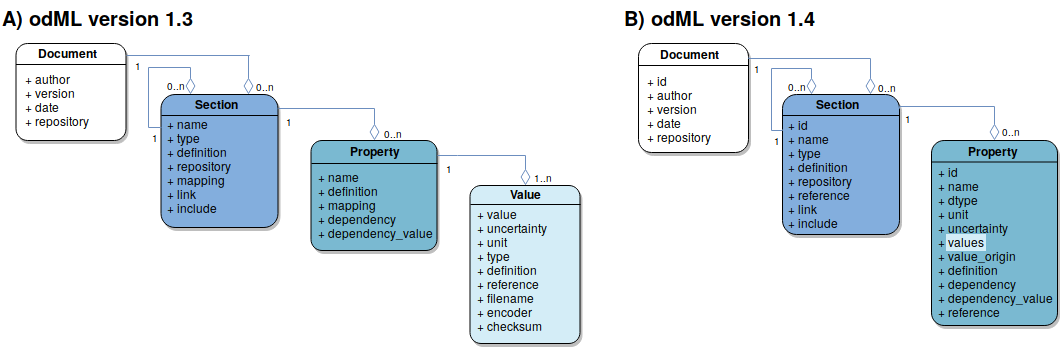
\includegraphics[width=1.0\columnwidth]{figures/odmltables_figures/fig3_odml_data_model/odML_DataModel_version.png}
    \caption[Evolution of the \software{odML} data-model]{\textbf{Evolution of the \software{odML} data-model.} Each box represents an entity defined by the data model and is color coded. Connections between entities are illustrated using the UML aggregation relation where a diamond denotes the target of a connection; the numbers at source and target denote the cardinality of each entity in the connection. (A) Version 1.3 data model. Four entities are defined: The \textit{Document} (marked in white) as the root element of a metadata file contains information about the author, document date, the document version and a default repository containing definitions used within the Document. It further contains grouping elements, \textit{Section}s (marked in dark blue). These are defined via their name and type attributes and can hold Subsections and provide semantic structure to an \software{odML} Document. The "definition" attribute provides information about the nature of a Section, while "link" and "include" refer to further Sections within the same or a different Document, respectively. Sections may contain named \textit{Property} entities (marked in cyan) which hold at least one \textit{Value} (marked in light blue) thus creating an extended key-value pair. (B) Version 1.4 data model: To simplify the use of the \software{odML} data model the Value entity was integrated into the Property taking over the attributes "dtype" (data type), "unit", "uncertainty", "value origin", and "reference". In this version a Property may contain a list of values, which must be identical in terms of the relocated attributes thus reducing the risk of ambiguities in the value list. For more information on attributes that have not been modified please refer to the original publication \citep{Grewe_2011}. Figure with permission adapted from \cite{Grewe_2011}.}
    \label{fig:odml_versions}
\end{figure}

\paragraph{Additional features}
The \software{odML} core library already provides an in-built mechanism to search and retrieve Sections, Properties or values within a Document. The need to consistently search for metadata entities across Documents from different sources led to the development of an export feature of \software{odML} metadata to the Resource Description Framework (RDF) format\footnote{\url{http://www.w3.org/TR/rdf-primer}}, a general and widely used storage format of graph databases. Multiple \software{odML} files exported to RDF can be loaded into any graph database supporting RDF and will be combined into a single graph. Moreover, while XML is still the default storage format, \software{odML} now additionally supports storing the metadata in the text based file formats JSON\footnote{\url{https://json.org}} and YAML\footnote{\url{https://yaml.org}}. JSON has become a de-facto data exchange standard between web based and standalone computer applications. The support of JSON makes \software{odML} metadata more easily consumable in machine-only workflows through modern applications. Since both XML and JSON primarily aim at machine-readability, their structure is not easily readable by humans. To ease reading of raw \software{odML} files by actual persons the YAML file format support was added.

For easy visualization and manipulation of specific \software{odML} files, the graphical user interface of \software{odMLtables} was integrated into the native \software{odML} GUI (odml-ui\footnote{\url{https://github.com/G-Node/odml-ui}}). Thus, the \software{odML} GUI now grants direct access to the main \software{odMLtables} features, making both software tools even easier to use back to back for both browsing and editing of metadata.


\subsection{Generic data organization via the \software{Nix} model}
The \software{Nix} model combines data and metadata in a common framework. For this six generic data objects are defined and combined with an \software{odML} based metadata structure. The \software{Nix} model is provided with a \software{C++} reference implementation\footnote{nixio \software{C++}, \url{https://nixio.readthedocs.io},  RRID:SCR\_016196} and bindings for \software{Java}, \software{Matlab}. An independent implementation in \software{Python} is provided\footnote{nixio / nixpy, Python, \url{https://pypi.org/project/nixio/}} with version $1.5.0b3$ being considered here.

The \software{Nix} model consists of two different types of object for the description of data and metadata. In total, there are six data and two metadata objects  described in the following (\ref{fig:intro_nix_model}).
Data values are caputured using \code{DataArray}s capable of holding any type of data that can be described using a single or multidimensional array. In addition to the values the \code{DataArray} also describes the physical properties of the stored values, e.g. the type of data, the physical unit of the values and a human readable label. Additionally the data array is connected to \code{Dimension} objects, providing details about each of the additional dimensions of the \code{DataArray} including also a label, the physical unit, a sampling interval and offset. With these two objects \software{Nix} captures all required data for a meaningful visualization of the stored data values (e.g. see \cref{fig:intro_nix_examples}). In addition, it offers objects for tagging subsets of the values stored in a \code{DataArray} and for describing the origin of the recording data. The first one is implemented as a \code{Tag} object, referencing a subset of the values in a \code{DataArray} and can be used to provide more information for a subset of values, e.g. the presentation of a stimulus or the labelling of a cell part. The second object is a \code{Source} object, which is used to track the origin of data. The remaining data object \code{Group} is used for logical grouping of other \software{Nix} data objects. All data objects are coordinated via \code{Block}, which again is together with the metadata objects grouped in a \software{Nix} \code{File} object, representing a complete dataset.
The metadata objects used in the \software{Nix} framework are taken from the \software{odML} framework. All data objects within \software{Nix}, except for the \code{Dimension} object, can link to a single \code{Section} in the metadata collection of the \software{Nix} \code{File}, which contains additional information about the data object. Depending on the declared types of the linked data and metadata object, this relation is interpreted mono- or bidirectional, i.e. the metadata \code{Section} enriches the data object or the metadata object is additionally also defined via the data object.

The \software{Nix} repository is accompanied with an extensive wiki\footnote{\software{Nix} wiki, \url{https://github.com/G-Node/nix/wiki}} and documentation\footnote{\software{Nix} documentation, \url{https://nixio.readthedocs.io}} including tutorials and demos, providing a simple start for new users.

The \software{Nix} model is natively integrated in the the electrophysiology recording system \software{RELACS}, the \software{EEGbase}\footnote{EEGbase, \url{http://eegdatabase.kiv.zcu.cz}, RRID:nif-0000-08190} a system for storage, management, sharing and retrieval of EEG data as well as \software{Neo}, a Python tool for standardized representation of electrophysiology data (\ref{sec:neo}).


\begin{figure}
 \centering
 \begin{minipage}[t]{0.8\textwidth}
 \textbf{A}\newline\\
 \hfill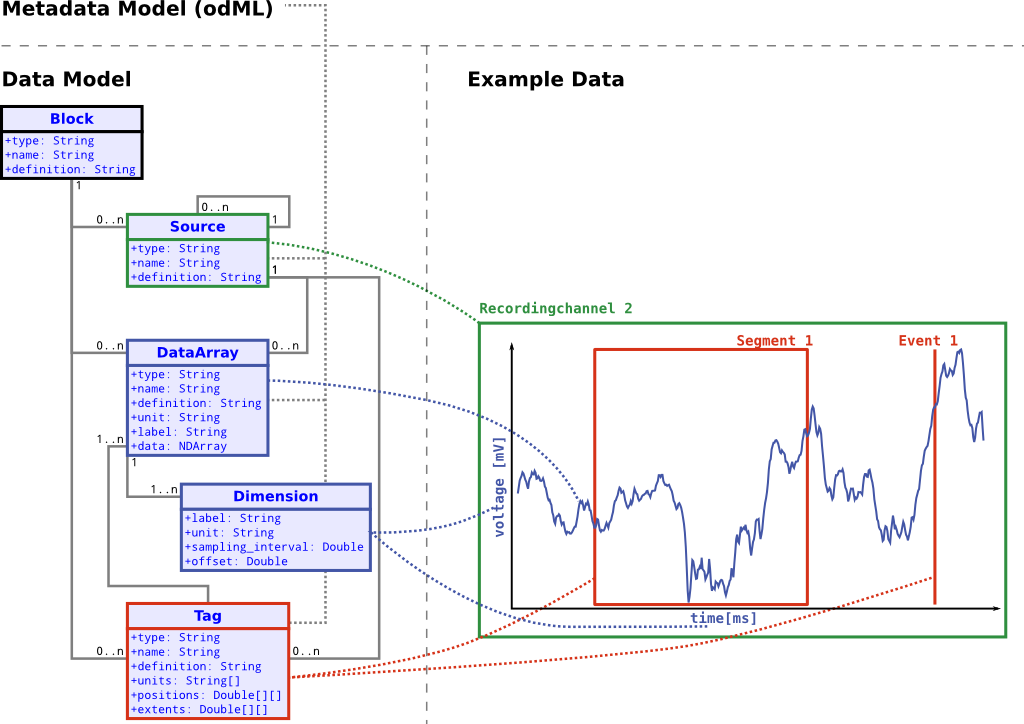
\includegraphics[width=0.9\textwidth]{./figures/introduction/pandora_example_signal}
 \end{minipage}\\
 \vspace{1cm}
 \begin{minipage}[t]{0.8\textwidth}
 \textbf{B}\newline\\
 \hfill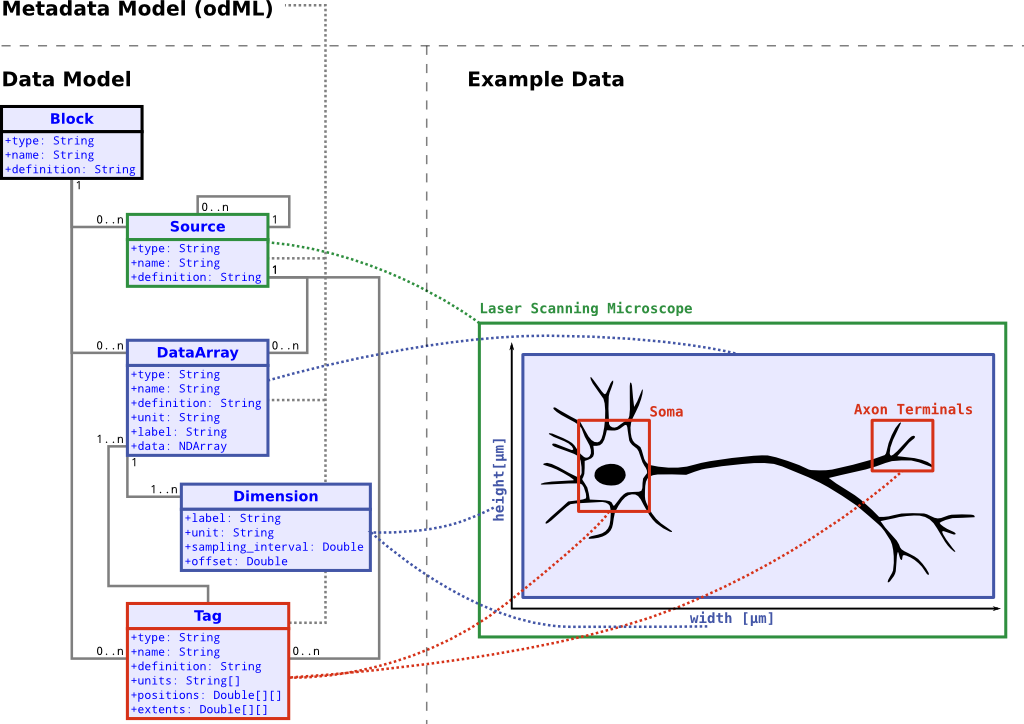
\includegraphics[width=0.9\textwidth]{./figures/introduction/pandora_example_image}
 \end{minipage}
 \caption[Nix model application examples]{Nix model application examples. The model can capture different varieties of data, e.g. electrophysiological recording traces (A) and imaging data (B). Both signals types can be mapped to the same types of objects of the \software{Nix} model. Figure from \software{Nix} documentation\footnote{\url{https://github.com/G-Node/nix/wiki/The-Model}}}
 \label{fig:intro_nix_examples}
\end{figure}

\begin{figure}
 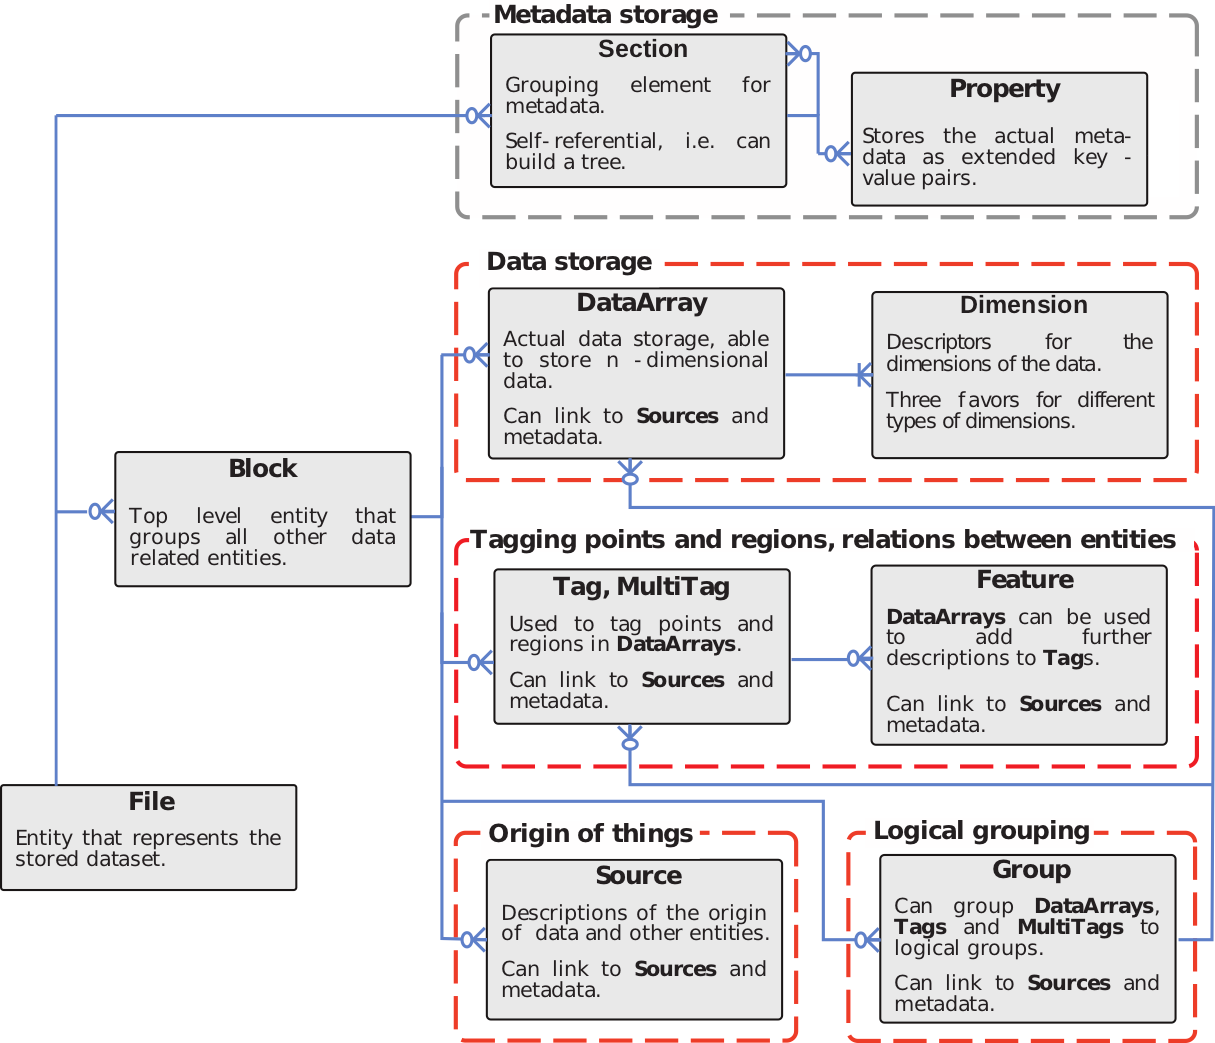
\includegraphics[width=0.9\textwidth]{./figures/introduction/data_model_brief_adapted}
 \caption[Nix model objects]{Nix model objects. The model consist of objects for storing data and metadata and relations between these. Metadata is captured in a \software{odML} based structure. Figure adapted from \software{Nix} documentation\footnote{\url{https://nixio.readthedocs.io/en/latest/data_model.html}}}
 \label{fig:intro_nix_model}
\end{figure}

\section{Thesis overview}
In \cref{sec:data} we describe two published datasets of a complex, collaborative electrophysiological experiment including an extensive metadata collection. We describe the process of data and metadata preparation required for the data publication and discuss the workflow used in this publication to identify strengths and shortcomings of the presented approach. In \cref{sec:metadata} we present odMLtables, a tool for facilitation of metadata collection compatible with the previously presented workflow. We demonstrate the embedding of odMLtables in a real-world metadata workflow and highlight the latest features and developments of the tool. \cref{sec:neo} complements the the previous section by introducing tools for standardized data representation and presents three example applications. \cref{sec:workflows} introduces modern workflow management software for efficient organization and structuring of scientific projects. We demonstrate the integration of the previously presented tools in a systematic fashion using modern workflow management software to coordinate the application of data and metadata software in a neuroscientific project. Finally, in \cref{sec:discussion} we discuss the presented approaches and provide an outlook on future development of the tools and concepts.





\clearpage
\chapter[Sharing data]{Sharing data\\- Publication of two complex electrophysiological datasets}
\label{sec:data}
\todo{integrate into big picture}
\todo{rewrite red parts}
\todo{proof read \& correct}

Scientific progress is the result of scientific findings that build on each other. To validate such findings, typically hypothesis are proposed and tested against experimental data using statistical methods. The resulting finding and interpretation is communicated to other scientists via the publication of a manuscript. In recent years, however, the practice of publishing papers has been criticized for a lack of robustness. Attempts in a number of scientific fields including life sciences, among others, to reproduce published scientific findings failed to support the same conclusions \citep{Baker_2016, Fidler_2017, Pashler_2012, Ioannidis_2005, Goodman_2007, Ioannidis_2007, OpenScienceCollaboration_2015}. To qualitatively distinguish between different levels of reproducibility, a collection of terms has been applied: reproducibility, replicability, repeatability \citep{Plesser_2018, Drummond_2009}. However the specific interpretation of each of these terms highly depends on the scientific field they are applied in. Repeatability, for example, can be defined as the re-performance of the same experimental study using identical components. However, for computer sciences repeating an experiment might be the re-running of the same software simulation on the same machine using the same software packages. In consequence, the feasibility of repeating a study highly depends on the field. For example repeating an study by running the same code on the identical machine might be a realistic project, whereas running the identical experiment in psychology is not \citep{Anderson_2016}. A widely accepted version of reproducibility terminology by \citet{Goodman_2007} is therefore omitting the terms 'replicability' and 'repeatability' for simplification and defines instead three different types of reproducibility \citep[from][]{Plesser_2018}:

\begin{minipage}{\textwidth}
\begin{description}
 \item[Methods reproducibility] \hfill \\ \textit{'provide sufficient detail about procedures and data so that the same procedures could be exactly repeated.'}
\item[Results reproducibility] \hfill \\ \textit{'obtain the same results from an independent study with procedures as closely matched to the original study as possible.'}
\item[Inferential reproducibility] \hfill \\ \textit{'draw the same conclusions from either an independent replication of a study or a reanalysis of the original study.'}\\
\end{description}
\end{minipage}

The definition of 'methods reproducibility' highlights a central aspect of scientific publications: the underlying data. Reproducing findings of publications is difficult for older publications \citep{Vines_2013,Rostami_2017}, which to a large part can be accounted for by the decreasing ability to retrieve of the original datasets. The obligation to provide research data to other scientists is a practice promoted by increasingly many funding organizations (e.g. NIH since 2003\footnote{\url{https://grants.nih.gov/grants/policy/data_sharing/}}, EU Horizon 2020 Open Research Data Pilot\footnote{\url{https://ec.europa.eu/research/participants/docs/h2020-funding-guide/cross-cutting-issues/open-access-data-management/data-management_en.htm}} since 2014) for publications in a number of journals (e.g. Springer Nature\footnote{\url{https://www.springernature.com/gp/authors/research-data-policy/data-availability-statements/12330880}}), however the readiness to comply is rather low (1/10 publications provides research data on request \citep{Savage_2009}. To address the problem of methods reproducibility for original research articles, a number of new journals were put into place, which invite to publish replications of the original articles in computational science \footnote{ReScience, \url{http://rescience.github.io/}}, economics\footnote{\url{http://www.economics-ejournal.org/special-areas/replications-1}}, psychology\footnote{\url{https://www.apa.org/pubs/journals/xge/replication-articles}} and neuroscience \citep{Yeung_2017} as well as original research data (e.g. ScientificData\footnote{ScientificData, \url{https://www.nature.com/sdata/}}.

To improve the situation of data availability, \citet{Wilkinson_2016} defined the FAIR Principles, a set of guidelines to achieve sustainable data and metadata management. The four key objectives are to make research data
\begin{quote}
\begin{description}
 \item[F]indable by generating unique and persistent identifiers for data and metadata files. This include the generation of a comprehensive metadata collection, clearly linked to the data via the identifier and vice versa. This way datasets and corresponding metadata can be registered and indexed and are findable via search queries.
 \item[A]ccessible by making data and metadata retrievable via their unique identifier in a standardized way. The applied standards and protocols should be open, free and universal and the accessibility of either data or metadata should not depend on the availability of the other. 
 \item[I]nteroperable by using standardized, broadly applicable tools and language for knowledge representation. This includes using FAIR terminology and providing qualified references to other metadata.
 \item[R]eusable by providing comprehensively described data and metadata including a clear licence statement, detailed provenance information using community standards. 
\end{description}
\end{quote}
 Complementing these guidelines, a number of sites have become available for hosting scientific data (Zenodo\footnote{Zenodo, \url{https://zenodo.org/}}, figshare\footnote{figshare, \url{https://figshare.com/}}, Pangaea\footnote{Pangaea, \url{https://www.pangaea.de}}, BMC Research Notes\footnote{BMC Research Notes, \url{https://bmcresnotes.biomedcentral.com/} \& \url{https://bmcresnotes.biomedcentral.com/about/introducing-data-notes}}, DataDryad\footnote{DataDryad, \url{https://datadryad.org/}}, GIN\footnote{GIN, \url{https://gin.g-node.org/}}, EuDat\footnote{EuDat, \url{https://eudat.eu/}}, Research Data Australia\footnote{RDA, \url{https://www.ands.org.au/online-services/research-data-australia/rda-registry}}, see also \citet{Assante_2016}) and publishing data descriptor papers (ScientificData\footnote{ScientificData, \url{https://www.nature.com/sdata/}}, DataScience\footnote{DataScience, \url{https://datascience.codata.org/}}, see also \citet{Candela_2015}).
It has been shown that mandated data archiving upon publication highly improves data availability \citep{Vines_2013}. However, a central prerequisite for the usability of the dataset is the existence of a comprehensive metadata collection \citep{Ferguson_2014,Parekh_2015,Ascoli_2017}. Going one step further, \citet{Chen_2019} show that making only the data (and metadata) available is not sufficient for reproducible science but rather, data also need to be accompanied by software packages used for further analysis. In the optimal case this encompasses a detailed, step-wise description of the motivation for an analysis workflow. \citet{Jomhari_2017} demonstrate that even for datasets surpassing commonly available hardware capabilities (e.g., due to memory limitations), e.g. from particle physics, making the effort of publishing the data is possible and can lead to successful reuse of the data.

The publication of a dataset adhering to the FAIR principles involves a number of concepts, but also technical tools to enable this process. To demonstrate what this entails in practice, here we report on our initial efforts to establish such knowledge for electrophysiology data in the context of the workflows established for a concrete data publication, and discuss critically that implementation. We provide an example of two complex published datasets from the field of neuroscience \citep{Brochier_2018}, demonstrating the richness of data and metadata involved in such an experiment and the concepts to prepare the data for analysis and publication. We present the pipeline used for metadata aggregation and discuss its strengths and shortcomings. Parts of the conceptual underpinnings of the pipeline are published in \citet{Zehl_2016} where they serve as example cases for metadata handling practices. In the following we describe the published datasets based on \citet{Brochier_2018}.



% \section{Publication of two complex electrophysiological datasets}
In \citet{Brochier_2018} we publish two complete high-dimensional electrophysiological datasets containing Utah Array recordings from monkey motor cortex. Recording subjects are two macaque monkeys (monkey L and N) which performed a complex instructed delayed reach-to-grasp task. Each recording contains continuously sampled data from 96 electrodes accompanied by the corresponding spiking activity. Spikes were extracted during online recording and offline sorted using the \software{Plexon Offline Sorter}\footnote{Plexon Offline Sorter, \url{https://plexon.com/products/offline-sorter/}}. Electrophysiological data are accompanied by a number of behavioral and control signals. Detailed metadata were aggregated and are provided in the \software{odML} format (see \cref{sec:intro,sec:scidata_metadata_structure}).

Complex datasets, as the two provided here (high-dimensional, multi-scale during complex behavior), are a challenge for performing reproducible analysis. Besides the often rather variable nature of the circumstances under which such data were recorded, the data additionally experience a number of often interactively performed preprocessing steps before they can be used in actual data analyses. Without a detailed knowledge about all these steps, the actual data analysis may be biased or strongly affected. In most cases, electrophysiological data available as open source are in this respect not sufficiently annotated and documented. For this reason, we provide here a comprehensive description of how and under which circumstances the datasets were recorded as well as a detailed description of preprocessing steps that need to be considered before performing analyses on the data. We additionally publish a machine-readable format of these metadata including our parameters and results of the described preprocessing steps. We are aware that all this information may not be sufficient for the reproducible analysis of such data. The reason is that reproducible workflows including the provenance trail are not yet established for electrophysiological neuroscience, especially not for such complex experiments as presented here.

\section{Relevance to the field}
The published datasets contain rare, multi-channel recordings from a complex electrophysiological setup. There are very few datasets of this type of experiment with this level of complexity available\footnote{published datasets from Utah array recordings in ScientificData: 1 \citep{Brochier_2018}, CRCNS.org: 1 (only spiking activity); date of access: 30 August 2019}, wherefore we provide a valuable addition to the collection of openly available datasets. The datasets are interesting for multiple reasons and can be used in a variety of contexts:
\begin{itemize}
 \item Public datasets are of high value for teaching and demonstration purposes. Especially for teaching it is important to not only work with toy examples, but having real-world data at hand. This improves the teaching quality and provides a better insight into the field. For teaching advanced analysis methods that analyse the correlative properties of neuronal dynamics, corresponding parallel data is essential, such as the provided dataset.
 \item For analysis of coordinated population activity of neural networks in the form of the local field (LFP) potential \citep{Mitzdorf_1985, Logothetis_2004, Einevoll_2013}, this datasets provides the opportunity to study LFP activity exhibiting wave activity across a spatially extended volume of cortex \citep{Denker_2018}.
 \item The datasets contain spiking activity from approximately 100 neurons recorded simultaneously. This permits analysis of coordinated spiking activity, e.g. via correlation analysis techniques \citep{Torre_2016, Torre_2016a, Quaglio_2017, Quaglio_2018}.
 \item The availability of LFP as well as spiking data invites to study the relation between the two modalities, e.g. by relating synchrony in spiking activity to beta band power in the LFP \citep{Denker_2011}.
 \item Additionally to spiking and LFP data the dataset is also rich in behavioural aspects, since the monkey is performing a complex commonly investigated delayed reach-to-grasp task \citep{Smeets_2019,Runnarong_2019}. These datasets provide the opportunity to relate the previously described neuronal analysis to the behaviour of the animal.
 \item The published datasets can serve as first application target for the development of new analysis methods for LFP and spiking activity. Especially needed are e.g. analysis methods applicable to hundreds and more simultaneously recorded spike trains since recent technical development rapidly increases the number of electrodes that can be recorded from in parallel. Most currently available methods are already approaching limits with respect to their demands for compute time and memory with current datasets due to combinatorial explosion \citep{Seo_2015,Jun_2017}. An example of methods that overcome combinatorial issues are dimensionality reduction methods like Gaussian-Process Factor Analysis (GPFA) \citep{Yu_2009}. 
 \item The published datasets together with the detailed description of metadata sources can serve as a template for development of a comprehensive metadata tracking system for neuroscientific experiments. Parts of this development are presented in later sections of this manuscript.
 \item The the correct identification of spikes based on a continuous recording trace (spike sorting) is a field of active research \citep{Rey_2015, Lefebvre_2016, Sukiban_2019}. For the evaluation of spike sorting algorithms, the availability of testing data is critical. With this dataset we provide raw recording traces, automatically extracted threshold crossing events as well as a manual spike sorting to compare new spike sorting algorithms to.
\end{itemize}


\section{The experiment}
The experiment is a delayed reach-to-grasp task performed by macaque monkeys. The basic components of the experiment are displayed in \cref{fig:r2g_introduction}. The monkeys are trained to attend two cues coding for the grip type and force to perform. After the second cue the monkey performs the movement, pulls the object and holds it to receive a reward. At the same time neuronal activity is recorded from motor and premotor areas of the cortex via a chronically implanted Utah Array. 

The subjects of the published datasets are two Rhesus macaque monkeys (Macaca mulatta) which were trained to perform the delayed reach-to-grasp task prior to implantation of the recording arrays. Details on the two subjects are summarized in \cref{tab:scidata_data_overview}. Depending on the monkey character and learning abilities, the different instruction steps (accustoming to the experimenter, setup, different versions of the task) require multiple months of daily training. The training was completed when the monkey had an average success rate of 85\% of the trials in the standard task setting.
The two monkeys trained for the task differ in gender, active hand of the task and character resulting in different behaviours observed during the recording task. As monkey N is rather calm and less motivated he is in general performing shorter sessions and less trials per session as monkey L, who is eager to work (see \cref{tab:scidata_data_overview}). A recording day typically consisted of multiple recording sessions, whereas each session lasts between $10$ and $20$ minutes resulting in an average working time per weekday of $1.5$ hours. Weekends and holidays were usually excluded from training and recording.

\begin{table}[]
\scriptsize
\begin{tabular}{|l|l|l|l|l|l|l|l|}
\hline
                                                                                              & \multicolumn{3}{l|}{\textbf{monkey L}}                                                                   & \multicolumn{3}{l|}{\textbf{monkey N}}                                                            & \textbf{description}                                                                             \\ \hline
\multicolumn{8}{|l|}{\textbf{Monkey}}                                                                                                                                                                                                                                                                                                                                                                           \\ \hline
gender                                                                                        & \multicolumn{3}{l|}{female}                                                                              & \multicolumn{3}{l|}{male}                                                                         &                                                                                                  \\ \hline
birth date                                                                                     & \multicolumn{3}{l|}{15th March 2004}                                                                     & \multicolumn{3}{l|}{15th May 2008}                                                                &                                                                                                  \\ \hline
weight                                                                                        & \multicolumn{3}{l|}{5kg}                                                                                 & \multicolumn{3}{l|}{7kg}                                                                          &                                                                                                  \\ \hline
active hand                                                                                   & \multicolumn{3}{l|}{left}                                                                                & \multicolumn{3}{l|}{right}                                                                        &                                                                                                  \\ \hline
character                                                                                     & \multicolumn{3}{l|}{\begin{tabular}[c]{@{}l@{}}eager to work\\ quick\\ efficient\\ nervous\end{tabular}} & \multicolumn{3}{l|}{\begin{tabular}[c]{@{}l@{}}slow learner\\ calm\\ less motivated\end{tabular}} &                                                                                                  \\ \hline
Utah array rotation                                                                           & \multicolumn{3}{l|}{216$^\circ$}                                                                          & \multicolumn{3}{l|}{239$^\circ$}                                                                   &                                                                                                  \\ \hline
\textbf{Recording}                                                                            &                                        &                                &                                &                                      &                              &                             &                                                                                                  \\ \hline
session name (*)                                                                              & \multicolumn{3}{l|}{\textbf{l101210-001}}                                                                & \multicolumn{3}{l|}{\textbf{i140703-001}}                                                         &                                                                                                  \\ \hline
session files                                                                                 & *.ccf                                  & \multicolumn{2}{l|}{108.2 kB}                                   & *.ccf                                & \multicolumn{2}{l|}{187.1 kB}                              & cerebus configuration                                                                            \\ \hline
                                                                                              & *.nev                                  & \multicolumn{2}{l|}{287.7 MB}                                   & .nev                                 & \multicolumn{2}{l|}{168.3 MB}                              & \begin{tabular}[c]{@{}l@{}}digital events\\ unsorted spikes times\\ spike waveforms\end{tabular} \\ \hline
                                                                                              & *-02.nev                               & \multicolumn{2}{l|}{287.7 MB}                                   & *-03.nev                             & \multicolumn{2}{l|}{168.3 MB}                              & \begin{tabular}[c]{@{}l@{}}digital events\\ sorted spikes times\\ spike waveforms\end{tabular}   \\ \hline
                                                                                              & *.ns2                                  & \multicolumn{2}{l|}{8.5 MB}                                     & *.ns2                                & \multicolumn{2}{l|}{204.7 MB}                              & \begin{tabular}[c]{@{}l@{}}analog signals of object sensors\\ LFP (only monkey N)\end{tabular}   \\ \hline
                                                                                              & *.ns5                                  & \multicolumn{2}{l|}{4.1 GB}                                     & *.ns6                                & \multicolumn{2}{l|}{5.8 GB}                                & raw neuronal signal                                                                              \\ \hline
                                                                                              & *.odml                                 & \multicolumn{2}{l|}{2.7 MB}                                     & *.odml                               & \multicolumn{2}{l|}{2.3 MB}                                & metadata                                                                                         \\ \hline
recording start                                                                               & \multicolumn{3}{l|}{Fr, 10th Dec 2010 10:50am}                                                           & \multicolumn{3}{l|}{Th, 3rd Jul 2014 10:41am}                                                     &                                                                                                  \\ \hline
recording duration                                                                            & \multicolumn{3}{l|}{11:49 min}                                                                           & \multicolumn{3}{l|}{16:43 min}                                                                    &                                                                                                  \\ \hline
daily recording id                                                                            & \multicolumn{3}{l|}{1}                                                                                   & \multicolumn{3}{l|}{1}                                                                            &                                                                                                  \\ \hline
\begin{tabular}[c]{@{}l@{}}number of recordings\\ same day\end{tabular}                       & \multicolumn{3}{l|}{9}                                                                                   & \multicolumn{3}{l|}{3}                                                                            &                                                                                                  \\ \hline
\begin{tabular}[c]{@{}l@{}}total daily \\ recording time\end{tabular}                         & \multicolumn{3}{l|}{01:28 h}                                                                             & \multicolumn{3}{l|}{00:51 h}                                                                      &                                                                                                  \\ \hline
\multicolumn{8}{|l|}{\textbf{Performance}}                                                                                                                                                                                                                                                                                                                                                                      \\ \hline
\begin{tabular}[c]{@{}l@{}}recorded trials\\ (total/error/\\ grip error/correct)\end{tabular} & \multicolumn{3}{l|}{204}                                                                                 & \multicolumn{3}{l|}{160}                                                                          &                                                                                                  \\ \hline
\begin{tabular}[c]{@{}l@{}}trials performance\\  correct/error (grip error)\end{tabular}      & 135                                    & \multicolumn{2}{l|}{69 (12)}                                    & 135                                  & \multicolumn{2}{l|}{19 (16)}                               &                                                                                                  \\ \hline
\begin{tabular}[c]{@{}l@{}}trial types\\  SG-LF/SG-HF\end{tabular}                            & 41                                     & \multicolumn{2}{l|}{30}                                         & 35                                   & \multicolumn{2}{l|}{35}                                    &                                                                                                  \\ \hline
\begin{tabular}[c]{@{}l@{}}trial types\\  PG-LF/PG-HF\end{tabular}                            & 31                                     & \multicolumn{2}{l|}{33}                                         & 35                                   & \multicolumn{2}{l|}{36}                                    &                                                                                                  \\ \hline
\multicolumn{8}{|l|}{\textbf{Spike sorting}}                                                                                                                                                                                                                                                                                                                                                                     \\ \hline
\# SUA                                                                                        & \multicolumn{3}{l|}{93}                                                                                  & \multicolumn{4}{l|}{156}                                                                                                                                                                             \\ \hline
\# MUA                                                                                        & \multicolumn{3}{l|}{49}                                                                                  & \multicolumn{4}{l|}{19}                                                                                                                                                                              \\ \hline
\# electrodes with SUA                                                                        & \multicolumn{3}{l|}{65}                                                                                  & \multicolumn{4}{l|}{78}                                                                                                                                                                              \\ \hline
\begin{tabular}[c]{@{}l@{}}\# electrodes with \\     SUA or MUA\end{tabular}                  & \multicolumn{3}{l|}{86}                                                                                  & \multicolumn{4}{l|}{89}                                                                                                                                                                              \\ \hline
\end{tabular}
\caption[Overview of subjects and recording sessions]{Overview of monkeys, recording session files and dates, spike sorting and monkey performance. The monkeys differ in gender, age, weight and active hand used for the task. Information is provided about individual recording files, sessions, performance of the monkey as well as single unit (SUA) and multi unit activity (MUA). \todo{add more descriptions in table and nicefy table}}
\label{tab:scidata_data_overview}
\end{table}

\begin{figure}[!ht]
\centering
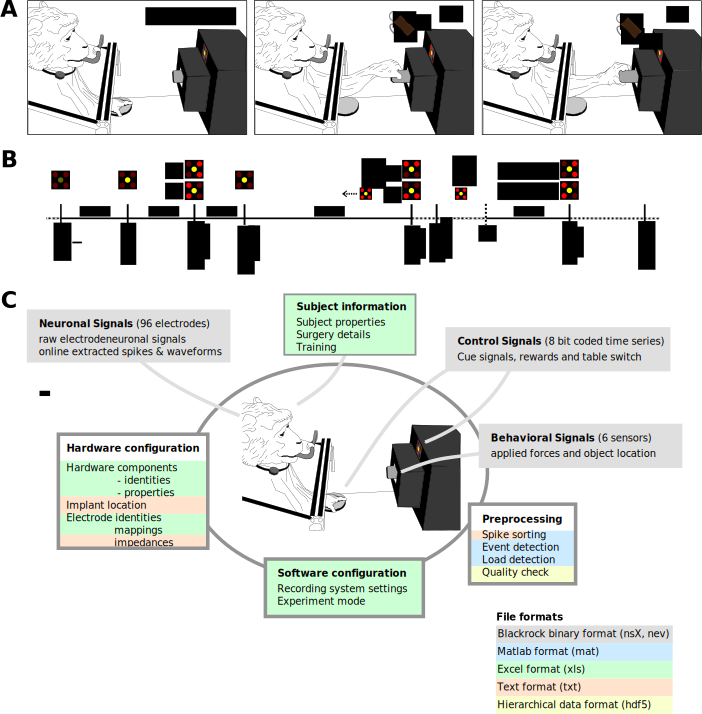
\includegraphics[width=\textwidth]{figures/scidata_experiment}
\caption[Components of the Reach-to-Grasp experiment]{Components of the Reach-to-Grasp experiment. A) The monkey is located in a monkey chair, his active hand resting the home position (left panel). The monkey performs an instructed, delayed reach towards an object. Two grip conditions (side grip/precision grip (SG/PG, respectively)) can be instructed via visual cues. B) Visual cues are presented via five LEDs located at the height of the monkeys eyes. The monkey initialized a trial by holding the home switch with his active hand for $400$ milliseconds, then the central LED is activated and stays active for the complete trial. Two complementary cues are presented with a delay of $1000$ milliseconds, coding for the grip type and the force needed to move the object. The of the four corner LEDs, always two neighboring ones are activated. The two vertical arrangements code for the grip type and the horizontal ones for the force type. After the second cue (GO-ON), the monkey releases the home switch (SR-ON), reaches for the object (hold start, HS) and holds it for $500$ milliseconds. Then a reward is delivered and the monkey can initiate the next trial by returning to the resting configuration and holding the home switch again. C) The data acquired during a recording session comprise neural activity signals, as well as behavioral and control signals. Metadata is captured in multiple formats, encompassing hard- and software components and settings as well as information about the subject and post-processing steps performed on the the data. Figure modified from \citet{Brochier_2018}.}
\label{fig:r2g_introduction}
\end{figure}

\begin{figure}
 \centering
 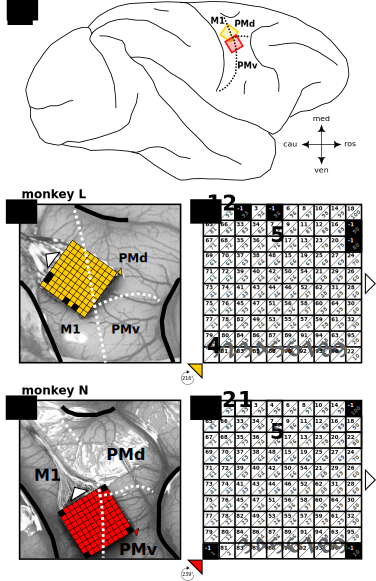
\includegraphics[width=0.65\textwidth]{./figures/scidata_figures/array_placements}
 \caption[Implant locations of the Utah arrays]{Implant locations of the Utah arrays. The figure displays the anatomical location of the Utah Array of both monkeys after implantation as well as the fabrication settings of each array provided by Blackrock. (a) Schematic drawing of a macaque cortex with implant location of the array of both monkeys. Both arrays were implanted along the central sulcus and overlapping the putative border (dotted line) between primary motor cortex (M1) and dorsal or ventral premotor cortex (PMd or PMv) of the right hemisphere. (b, d) Exact location of the array for each monkey in the close-up picture of the implantation site taken during the surgery (length of an array side is $4\textnormal{mm}$). The central sulcus, the arcuate sulcus and the superior precentral dimple are emphasized as thick black lines (to the left, right and top, respectively). (c, e) Scheme of each array in a default array orientation where the wire bundle (indicated with white triangles in (b-e)) to the connector points to the right. Each array scheme shows the 10-by-10 electrode grid with the electrode identification numbers (IDs) defined by Blackrock (black numbers) and the location of the non-active electrodes (indicated in black as $ID=-1$). Gray numbers show an alternative set of connector-aligned electrode IDs, assigned based on electrode location with respect to the connector of the array, which are more practical for data analysis and comparisons across monkeys. In order to best cover the arm/hand representation of the primary motor cortex, each array was rotated for the implantation. The center of rotation is indicated by a colored triangle (b-e), stating below (in c and e) the degree of rotation for each array.}
 \label{fig:implant_locations}
\end{figure}




For recording of neural activity, each monkey had a single Utah array\footnote{Blackrock Microsystems, Salt Lake City, UT, USA} implanted in the motor cortex contralateral to the active hand. The Utah array is an electrode array with 100 electrodes arranged in a $10\times10$ grid. 96 of 100 of the iridium coated electrodes can be used for recording (\cref{fig:implant_locations}). The individual electrodes are $1.5\textnormal{mm}$ long, $400\mu\textnormal{m}$ apart and have an average pre-implantation impedance of $50\textnormal{k}\Omega$. The electrode array is connected to a head stage via a fiber bundle connecting individual electrodes to the contact of the CerePort Connector, which is a connector external to the skin permitting the daily coupling of the implant to the recording setup. In addition to the array electrodes one ground and two reference electrodes are implanted. During the implantation surgery the skull was opened and the dura removed to pneumatically insert the Utah array into the cortex. The dura and skull were close, whereby the cables were arranged to lead to the connector which was attached to the skull on the other hemisphere. The Utah arrays were implanted a few millimeters anterior to the central sulcus and they were rotated before implantation to cover the arm/hand representation of the primary motor cortex as well as parts of premotor cortex (\cref{fig:implant_locations}).

The task the monkeys had to perform involved grasping an object using one of two grip types: side (SG) or precision grip (PG). Detailed sketches of the different grips are depicted in   \cref{fig:r2g_introduction}A center and top panel. For both grip types the position of thumb (T), index (I) and middle (M) finger are indicated relative to the profile of the object. The force required to pull the object towards the monkey was either about $1\textnormal{N}$ (low force) or $2\textnormal{N}$ (high force).  In a trial the monkey was always instructed by the first cue (CUE) about the grip type (SG/PG) and with the second cue (GO) about the force level (LF/HF), resulting in 4 different trial types (SGLF, SGHF, PGLF, PGHF) possible (\cref{fig:task_trialscheme}). The first and second cue are presented with $1\textnormal{s}$ delay in which the monkey has to memorize the presented grip type and can prepare for the movement, which can be initialized after the second (GO) cue. Cues are presented by combinations of two of five illuminated LEDs. The encoding of the grip and force type can be seen in \cref{fig:r2g_introduction}B (CUE-ON and GO-ON). The setup consisted of three main parts, the neural recording platform for acquisition of neuronal signals, the experimental apparatus providing the environment for performing the task and the behavioral control system controlling and coordinating the task procedure (\cref{fig:scidata_setup_overview}).

\paragraph{Differences between the datasets}
In principle, the same setup was used for both monkeys, however, small deviations exist which are highlighted in the corresponding \cref{fig:implant_locations,fig:scidata_setup_overview,fig:cerebus_system} in yellow (monkey L) and red (monkey N). The four main aspects are
\begin{description}
 \item[Recording Arrays] The datasets are recorded using different Utah arrays. This includes a different electrode mapping as well as a different implant location.
 \item[Connecting Hardware] Usage of different hardware for connecting the implant with the data acquisition system. The two headstages (samtec/patient cable) influence the recording quality by their specific electrical properties.
 \item[Software versions and settings] The recording software versions and setting differ, since an update was available between the recordings. This includes the usage of different file extensions for recordings of continuous data (ns5 in monkey L vs ns6 in monkey N) and additionally a downsampled and filtered version of the neural data being recorded in parallel in the ns2 format for monkey N, which was not available by the software for monkey L. Furthermore the number of samples extracted online for each of the threshold crossing events was increased from 39 samples in monkey L to 48 samples in monkey N.
 \item[Experiment Control] The LabView program controlling and monitoring the task was updated which leads to the usage of different binary coding for digital events (\cref{tab:bit_translation}). 
\end{description}




\begin{figure}
 \centering
 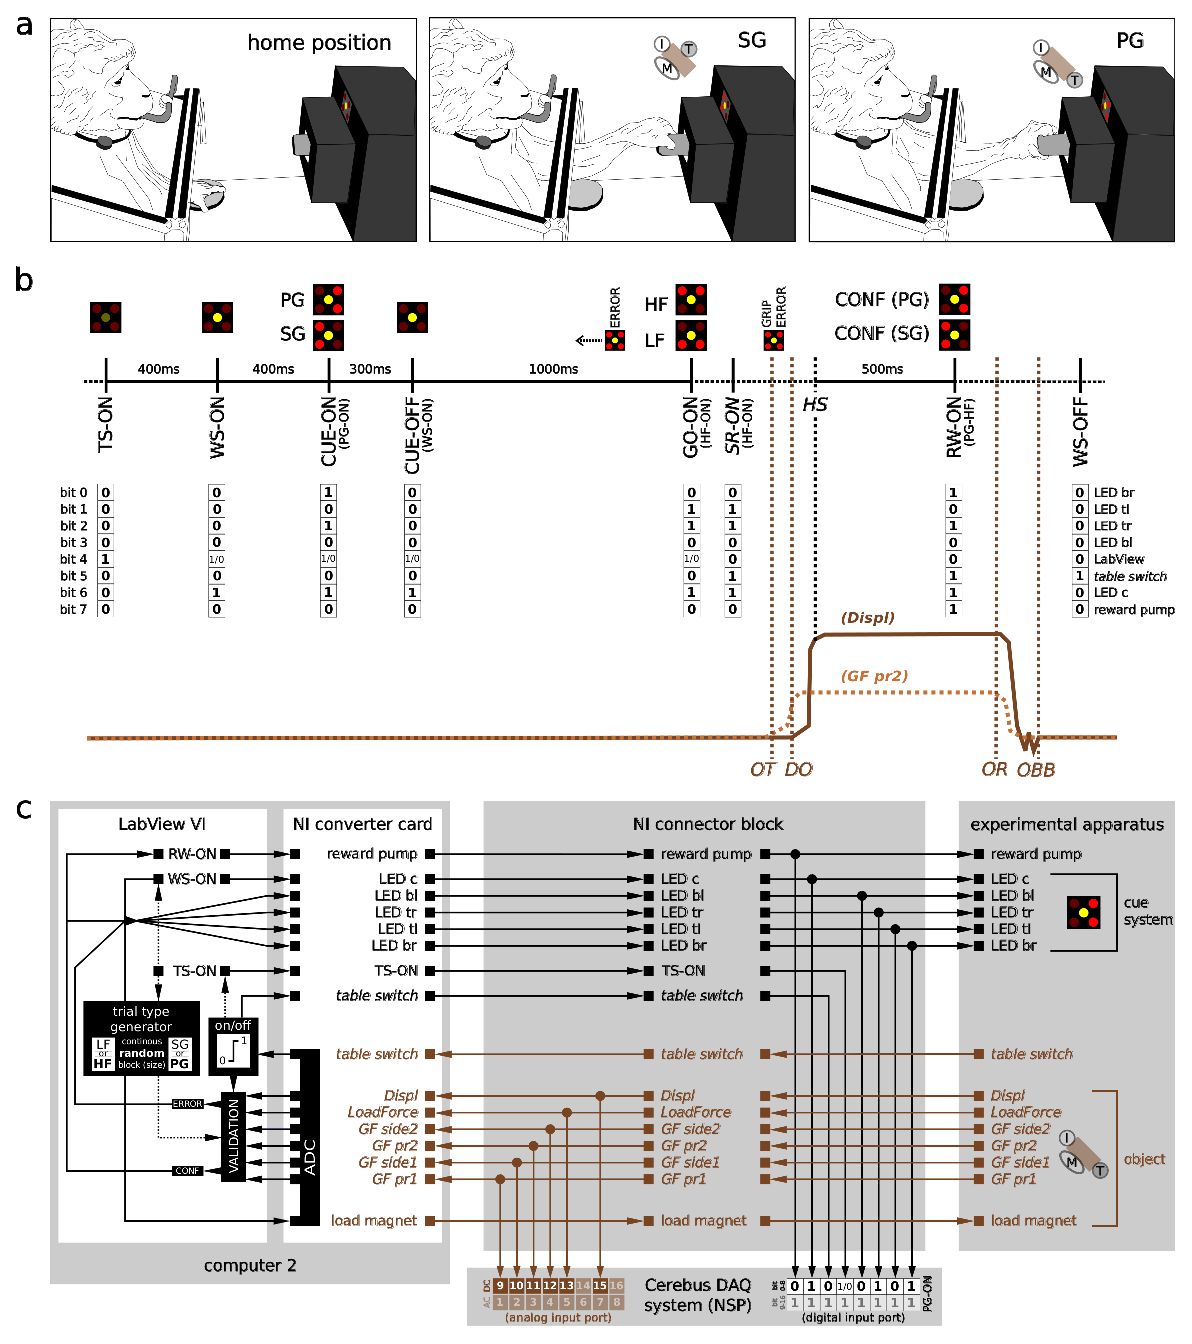
\includegraphics[width=0.8\textwidth]{./figures/scidata_figures/task_trialscheme}
 \caption[Overview of the experimental apparatus and behavioral control system.]{Overview of the experimental apparatus and behavioral control system. (a) Sketches of the experimental apparatus and the monkey performing the reach-to-grasp task. Left: monkey in its home position with the working hand on the table switch. Middle and right: monkey grasping the object with a side grip (SG) and a precision grip (PG), respectively. Insets of middle and right sketch show the actual position of the index finger (I), the thumb (T), and the middle finger (M) on the object (brown cube) 11 . (b) Trial scheme of an example trial with
the respective visual cues (different illumination combinations of the 5 LEDs illustrated on top) shown to the monkey at its respective times. The behavioral events are marked along the time axis (see main text for abbreviations). \code{Event}s with black font mark digitally recorded events, whereas events with brown font indicate events (object touch OT, object release OR, displacement onset DO, and object back to baseline OBB) which were extracted offline from baseline deviations of the analog signals of the object’s sensors. Additionally, we indicate by italic fonts events which were generated by the monkey, while all other events are produced by LabView. The 8-bit binary code for the digital event signals sent from LabView VI to the NSP at the respective times is shown below the time axis. Example traces for the analog signals of the HE sensor (Displ; dark solid line) and one of the 4 FSR sensors located at the object’s surface (GF pr2, light dotted line) used to monitor the monkeys behavior and extract
OT, OR, DO, and OBB are shown at the bottom. (c) Outline of the devices and their wiring controlling the behavior. All analog signal streams are colored in brown, whereas all digital signal streams are colored in black.}
\label{fig:task_trialscheme}
\end{figure}


\begin{figure}
 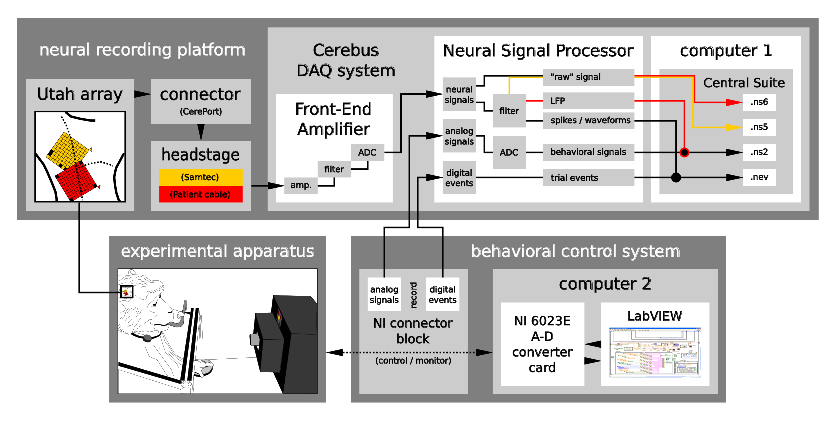
\includegraphics[width=\textwidth]{./figures/scidata_figures/setup_overview}
 \caption[Overview of the setup]{Overview of the setup. The setup consisted of three main parts: the neural recording platform, the experimental apparatus, and the behavioral control system. The neural recording platform (top) was composed of the implanted Utah array with its corresponding connector (CerePort), a headstage (Samtec or Patient cable), and the Cerebus data acquisition (DAQ) system (i.e. the Front-End Amplifier, Neural Signal Processor (NSP), and the Cerebus control software, Central Suite, installed on the setup computer 1). The experimental apparatus (bottom left) consisted of the physical devices which the monkeys had to interact with (i.e., the visual cue panel (square with 5 LEDs), the target object, the table switch, and the reward system). The behavioral control system (bottom right) was built from hard- and software of National Instruments (NI, National Instruments Corporation, Austin, Texas, USA). It was composed of a NI connector block which was linked via a NI 6023E A-D converter card to setup computer 2 on which the NI system design software, LabView, was running. To record the behavioral data the behavioral control system was interlinked with the neuronal recording platform via the NSP and the NI connector block. All three parts are separately described in more detail in the main text, as well as Figures 2 and 4. Setup differences between the two monkeys are indicated in yellow and red for monkeys L and N, respectively.}
 \label{fig:scidata_setup_overview}
\end{figure}

\begin{table}[]
\footnotesize
\begin{tabular}{|l|l|l|l|l|l|}
\hline
sensor & channel ID & label     & located at       & activated by          & used to identify  \\ \hline
FSR 1  & 137        & GF pr1    & object’s top     & index finger’s touch  & PG type           \\ \hline
FSR 2  & 138        & GF side1  & object’s left    & middle finger’s touch & SG type           \\ \hline
FSR 3  & 139        & GF pr2    & object’s bottom  & thumb touch           & PG type           \\ \hline
FSR 4  & 140        & GF side2  & object’s right   & thumb touch           & SG type           \\ \hline
FSR 5  & 141        & LoadForce & object’s spring  & object loading        & pulling force     \\ \hline
HE     & 143        & Displ     & object's shuttle & object displacement   & object’s position \\ \hline
\end{tabular}
 \caption[Overview of six objects sensors to monitor and control the monkey's behavior]{Overview of the six object sensors used to monitor and control the monkey's behavior. The first four force sensitive resistance (FSR) sensors are used to monitor the applied grip type. They are located on the surface of each object side and are activated by the touch of the corresponding monkey's finger. The fifth FSR is located at the spring counterbalancing the pull resistance of the object and is used to measure the pulling force applied by the monkey. The hall-effect sensor (HE) is located along the low-friction shuttle of the object and used to measure the position of the object. The signals of all sensors are saved in the ns2 with the stated channel ID and label (cf. \cref{fig:cerebus_system}).}
 \label{tab:overview_sensors}
\end{table}

\begin{table}[]
\scriptsize
\begin{tabular}{|l|l|l|l|l|l|l|l|l|l|c|l|}
\hline
\textbf{\begin{tabular}[c]{@{}l@{}}decimal\\ code\end{tabular}} & \multicolumn{8}{c|}{\textbf{(8-bit) binary code}}                                                                                                                                                                           & \multicolumn{3}{c|}{\textbf{trial interpretation}}                                                 \\ \hline
                                                                & bit 7         & bit 6                           & bit 5           & bit 4       & bit 3                            & bit 2                            & bit 1                            & bit 0                            & \multicolumn{2}{l|}{}                                                                     & monkey \\ \hline
\textbf{65296}                                                  & 0             & 0                               & 0               & 1           & 0                                & 0                                & 0                                & 0                                & \multicolumn{2}{l|}{\textbf{TS-ON}}                                                       & L,N    \\ \hline
\textbf{65280}                                                  & 0             & 0                               & 0               & 0           & 0                                & 0                                & 0                                & 0                                & \multicolumn{2}{l|}{\textbf{TS-OFF}}                                                      & L      \\ \hline
\textbf{65344}                                                  & 0             & 1                               & 0               & 0           & 0                                & 0                                & 0                                & 0                                & \multicolumn{2}{c|}{\multirow{2}{*}{\textbf{WS-ON}}}                                      & L      \\ \cline{1-9} \cline{12-12} 
\textbf{65360}                                                  & 0             & 1                               & 0               & 1           & 0                                & 0                                & 0                                & 0                                & \multicolumn{2}{c|}{}                                                                     & N      \\ \hline
\textbf{65360}                                                  & 0             & 1                               & 0               & 1           & 0                                & 0                                & 0                                & 0                                & \multirow{2}{*}{\textbf{PG-ON}}                      & \multirow{4}{*}{\textbf{(CUE-ON)}} & L      \\ \cline{1-9} \cline{12-12} 
\textbf{65365}                                                  & 0             & 1                               & 0               & 1           & 0                                & 1                                & 0                                & 1                                &                                                      &                                    & N      \\ \cline{1-10} \cline{12-12} 
\textbf{65354}                                                  & 0             & 1                               & 0               & 0           & 1                                & 0                                & 1                                & 0                                & \multirow{2}{*}{\textbf{SG-ON}}                      &                                    & L      \\ \cline{1-9} \cline{12-12} 
\textbf{65370}                                                  & 0             & 1                               & 0               & 1           & 1                                & 0                                & 1                                & 0                                &                                                      &                                    & N      \\ \hline
\textbf{65344}                                                  & 0             & 1                               & 0               & 0           & 0                                & 0                                & 0                                & 0                                & \multicolumn{2}{l|}{\multirow{2}{*}{\textbf{CUE-OFF}}}                                    & L      \\ \cline{1-9} \cline{12-12} 
\textbf{65360}                                                  & 0             & 1                               &                 & 1           & 0                                & 0                                & 0                                & 0                                & \multicolumn{2}{l|}{}                                                                     & N      \\ \hline
\textbf{65353}                                                  & 0             & 1                               & 0               & 0           & 1                                & 0                                & 0                                & 1                                & \multirow{2}{*}{\textbf{LF-ON}}                      & \multirow{4}{*}{\textbf{(GO-ON)}}  & L      \\ \cline{1-9} \cline{12-12} 
\textbf{65369}                                                  & 0             & 1                               & 0               & 1           & 1                                & 0                                & 0                                & 1                                &                                                      &                                    & N      \\ \cline{1-10} \cline{12-12} 
\textbf{65350}                                                  & 0             & 1                               & 0               & 0           & 0                                & 1                                & 1                                & 0                                & \multirow{2}{*}{\textbf{HF-ON}}                      &                                    & L      \\ \cline{1-9} \cline{12-12} 
\textbf{65366}                                                  & 0             & 1                               & 0               & 1           & 0                                & 1                                & 1                                & 0                                &                                                      &                                    & N      \\ \hline
\textbf{65385}                                                  & 0             & 1                               & 1               & 0           & 1                                & 0                                & 0                                & 1                                & \multirow{2}{*}{\textbf{SR}}                         & \multicolumn{1}{l|}{(+LF)}         & L,N    \\ \cline{1-9} \cline{11-12} 
\textbf{65382}                                                  & 0             & 1                               & 1               & 0           & 0                                & 1                                & 1                                & 0                                &                                                      & \multicolumn{1}{l|}{(+HF)}         & L,N    \\ \hline
\textbf{65509}                                                  & 1             & 1                               & 1               & 0           & 0                                & 1                                & 0                                & 1                                & \multirow{2}{*}{\textbf{RW-ON}}                      & \multicolumn{1}{l|}{(+CONF-PG)}    & L,N    \\ \cline{1-9} \cline{11-12} 
\textbf{65514}                                                  & 1             & 1                               & 1               & 0           & 1                                & 0                                & 1                                & 0                                &                                                      & \multicolumn{1}{l|}{(+CONF-SG)}    & L,N    \\ \hline
\textbf{65376}                                                  & 0             & 1                               & 1               & 0           & 0                                & 0                                & 0                                & 0                                & \multicolumn{2}{l|}{\textbf{GO-OFF/RW-OFF}}                                               & L,N    \\ \hline
\textbf{65312}                                                  & 0             & 0                               & 1               & 0           & 0                                & 0                                & 0                                & 0                                & \multicolumn{2}{l|}{\multirow{2}{*}{\textbf{STOP}}}                                       & L,N    \\ \cline{1-9} \cline{12-12} 
\textbf{65280}                                                  & 0             & 0                               & 0               & 0           & 0                                & 0                                & 0                                & 0                                & \multicolumn{2}{l|}{}                                                                     & L      \\ \hline
\textbf{65391}                                                  & 0             & 1                               & 1               & 0           & 1                                & 1                                & 1                                & 1                                & \multicolumn{1}{c|}{\multirow{2}{*}{\textbf{ERROR}}} & \multirow{2}{*}{(+switch)}         & L      \\ \cline{1-9} \cline{12-12} 
\textbf{65359}                                                  & 0             & 1                               & 0               & 0           & 1                                & 1                                & 1                                & 1                                & \multicolumn{1}{c|}{}                                &                                    & L      \\ \hline
\multirow{2}{*}{}                                               & \textbf{pump} & \textbf{LED}                    & \textbf{switch} & \textbf{TS} & \multicolumn{4}{c|}{\textbf{LED}}                                                                                                         & \multicolumn{3}{l|}{\multirow{2}{*}{}}                                                             \\ \cline{2-9}
                                                                &               & \multicolumn{1}{c|}{\textbf{c}} & \multicolumn{2}{c|}{}         & \multicolumn{1}{c|}{\textbf{bl}} & \multicolumn{1}{c|}{\textbf{tr}} & \multicolumn{1}{c|}{\textbf{tl}} & \multicolumn{1}{c|}{\textbf{br}} & \multicolumn{3}{l|}{}                                                                              \\ \hline
\end{tabular}
\caption[Translation table of 8-bit binary to decimal event codes and their interpretation in a trial context]{Translation table of 8-bit binary to decimal event codes and their interpretation in a trial context. The 8-bit binary event code created by LabView states the activation (bit status 1) and deactivation (bit status 0) of the LEDs of the cue system (c:center, t:top, b:bottom, l:left, r:right), the table switch (switch), the reward pump (pump) or the trial start (TS) internally set by LabView. During each trial the (8-bit binary) status of these devices/settings (cf. bottom row) were sent from LabView to the NSP of the Cerebus DAQ system (Figure 2). There, the event codes were converted to a decimal code of the bit sequence assuming another byte with all bits set to 1 in front. The decimal event codes are found in the nev files with a time stamp. The correct interpretation of these events in context of a trial are here indicated in the second column from the right. Due to different versions of the LabView control program for monkey L and N the decimal codes for the same event may differ between the monkeys (cf. first column from the right). Some event codes (65381, 65386, 65390, 65440, 65504) are not listed here, because they do not have a concrete meaning and occur only sporadically in the nev file due to a mistake in the sampling of the digital events - they have to be ignored. Except for the "ERROR" codes, the event codes are sorted in sequential order from top to bottom with respect to the task, i.e. their order corresponds to the sequence found in the nev file in a reach-to-grasp trial. Note that some events are represented by the same decimal codes and are just differently interpreted due to their sequential occurrence in a trial (cf. TS-OFF and STOP, as well as WS-ON and CUE-OFF).}
\label{tab:bit_translation}
\end{table}

\begin{figure}
 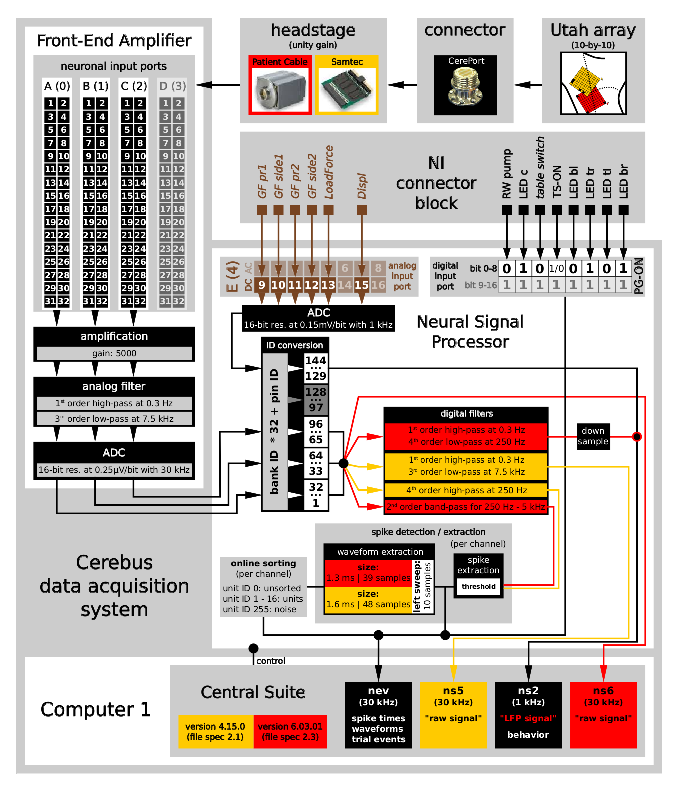
\includegraphics[width=0.7\textwidth]{./figures/scidata_figures/cerebus_system}
 \caption[Sketch of the components related to the recording of the neuronal signals]{Sketch of the components related to the recording of the neuronal signals. Data were recorded
using a Utah array, which was linked via its connector (CerePort) to a headstage (Samtec or Patient Cable) with a unity gain. From there the neural signals were transferred to the Cerebus Front-End Amplifier, where they were amplified, filtered and digitized. The digitized signals were converted into a single multiplex optical output and sent via a fiber-optic data link to the Neural Signal Processor (NSP), which is controlled by the Cerebus control software (Central Suite). Within the NSP the time points and waveforms of potential spikes were extracted online from a correspondingly processed copy of the neural signals and saved in the nev file. Simultaneously, the continuous raw signals (sampled at 30 kHz) were saved in the ns5 (for monkey L) or ns6 file (for monkey N). In parallel to the neural signals the NSP received also the digital trial events produced by the LabView VI, and the analog signals of the object’s sensors via the NI connector block of the behavioral control system. While the digital trial events were saved along with the extracted potential spikes in the nev file,
the analog signals of the sensors were digitized and saved in the ns2 file. For monkey N, a filtered and downsampled version of the neural signals (0.3–250 Hz at 1 kHz) was also saved in the ns2 file. Components and settings specific to monkey L and N are indicated by yellow and red, respectively.}
\label{fig:cerebus_system}
\end{figure}



\rewrite{

\section{Experimental apparatus}
\label{sec:experimental_apparatus}

The experimental apparatus was composed by a target object, a table switch, a visual cue, and a reward system. On each recording day, the monkey was seated in a custom-made primate chair and placed in front of that apparatus. The non-working arm of the monkey was loosely restrained in a semi-flexed position. To control the home position of the working hand between the reach-to-grasp movements, the table switch which was installed close to the monkey at waist level, 5cm lateral to the mid-line, needed to be pressed down. The target object was a stainless steel rectangular cuboid (40mm x 16mm x 10mm) rotated 45 degrees around the horizontal axis and pointing towards the monkey (\cref{fig:task_trialscheme}a). It was located 13cm away from the table switch at 14cm height. The posterior end of the object was attached through a low-friction horizontal shuttle to a counterweight hidden inside the apparatus, which was used to set the object load. The object load was set to one of two possible values to define the force type (LF and HF) needed for pulling the object in each trial by deactivating and activating an electromagnetic weight resting below the counterweight inside the apparatus. When activated, it attached to the counterweight and increased overall weight from usually 100gram to 200gram, which corresponds roughly to a pulling force of 1Newton and 2Newton for LF and HF, respectively. 

As already mentioned, the object was equipped with six sensors which monitored the monkey's reach-to-grasp behavior. Four force sensitive resistance sensors (FSR sensors) on the object surface provided continuous measurement of the grip forces applied on the object sides by the index and middle finger, as well as the thumb. The different activation patterns of these four FSR sensors, in particular the different placement of the thumb (see \cref{fig:task_trialscheme} a), were used to detect online if the correct grip type was performed. An additional FSR sensor was installed between the object and its counterweight. This FSR sensor was used to measure the horizontally applied force needed to oppose the corresponding object load. Due to the low, but still existing friction of the object moving inside the horizontal shuttle, the measured force signal of this sensor is not perfectly proportional to the horizontal force needed to lift the opposed object load, but sufficient to distinguish between LF and HF settings (cf., example in bottom right panel of \cref{fig:overview_data_l_1} and \cref{fig:overview_data_n_1}). The horizontal displacement of the object over a maximal distance of 15mm was measured by a hall-effect (HE) sensor. All sensors of the object are summarized in \cref{tab:overview_sensors}. The visual cue system, composed of a square of five LEDs (size 10 x 10 mm), was located just above the target object and used to instruct the monkey about the requested behavior. While the central yellow LED was used to warn the monkey that a trial had started, the four red corner LEDs were used to code separately the grip and the force type for the requested trial type of each trial. In this context the illumination of the two left, the two right, the two bottom, or the two top LEDs coded for SG, PG, LF, or HF, respectively (see \cref{fig:task_trialscheme} b for illustration). The reward system consisted of a bucket filled with apple sauce and equipped with a feeding tube and a pump allowing to deliver on demand the reward (few drops of the apple sauce) to the monkey (\cref{fig:task_trialscheme} a).

\subsection{Behavioral control system}
\label{sec:behavioral_control_system}

The core of the behavioral control system is a custom-made Virtual Instrument (VI) in LabView that controls the digital event sequence and the requested behavior of each trial in a recording. A digital event reflects hereby the activation or deactivation of a physical device of the experimental apparatus. In this context, the LabView VI is responsible to activate and deactivate the LEDs of the visual cue system, the reward pump, and the electromagnet. The latter is not controlled by a digital event, but by an analog square signal that switches the magnet on or off. To control the requested behavior, the LabView VI monitors the monkey's manipulation of the table switch and the target object. The table switch as well as all sensors of the target object produce continuous analog signals that are digitized by the NI converter card and fed into the LabView VI of the setup computer (see \cref{fig:scidata_setup_overview} computer 2). The square signal of the table switch is then online reinterpreted as digital activation or deactivation event. \cref{fig:task_trialscheme} c displays a schematic diagram on how the physical devices of the experimental apparatus are connected to the setup computer and controlled and monitored by the LabView VI. We will now describe a typical execution of the LabView VI during a recording session in more detail. 

The possible trial types were set to SG-LF, SG-HF, PG-LF, and PG-HF, alternating with equal probability randomly in sequence between trials. Once the settings of the overall task were defined, the LabView VI was started to repetitively run and control the event sequence and behavior for each trial during the recording session. 

Each single trial was run and controlled as follows: 

The LabView VI only started a trial when the monkey deactivated the table switch by pressing and holding it down (home position, \cref{fig:task_trialscheme} a, left). This required not much muscle activity, but simply the weight of the monkey's hand on top of the smooth-running switch. If the table switch was deactivated, the LabView VI internally initiated a trial with a short time delay (TS-ON). In parallel, the program picked randomly one of the possible trial types (e.g., SG-HF) and activated or deactivated the electromagnet accordingly to fit the chosen load force of the object (e.g., activated for HF). To inform (or warn) the monkey that a new trial has started, the central LED was illuminated 400ms after the trial was initiated by the program (WS-ON). Four hundred ms after WS-ON the grip type was revealed to the monkey by illuminating the corresponding corner LEDs of the chosen trial type (CUE-ON, e.g., left LEDs for SG-ON). The LEDs of this first cue were turned off again after 300ms (CUE-OFF). The CUE-OFF was followed by a 1000ms preparatory delay at the end of which the monkey was informed about the upcoming force type by again illuminating the corresponding corner LEDs of the chosen trial type (GO-ON, e.g., top LEDs for HF-ON). This second cue also served as a GO signal for the monkey to initiate the movement which was registered by the activation of the table switch (SR-ON) when the monkey released it after a variable reaction time (RT). The execution of the movement was composed of reaching, grasping, pulling and holding the object in the position window for 500ms. The LabView VI controlled the movement execution online by checking the used grip type, the object displacement and the hold time. For checking the grip type, the grasp of the object was registered by small deflections of the FSR surface sensor signals caused by the monkey's fingers. A FSR sensor was registered as activated if the deflection surpassed a predefined threshold. The pattern of activated FSR sensors was then used by the LabView VI to control if the monkey performed the requested grip type. This meant, in particular, to check for SG and PG, if the FSR sensor on the right (GF side2), or on the bottom (GF pr2) of the object was activated by the monkey's thumb, respectively (see \cref{fig:task_trialscheme} a, middle and right). The other 2 sensors that measured force from the index and middle fingers for the 2 grip types (GF side1, and GF pr1) were not controlled online. If the correct grip was detected, the grip cue was illuminated again as a positive feedback. To check the object displacement, the LabView VI measured if the deflection of the HE sensor signal of the object was within the two defined position thresholds (4 and 14mm). The time point at which the displacement signal surpassed the lower threshold was used by the LabView VI to define the estimated start of the holding period (HS) online. If the object remained within the position window for 500ms after the HS was set, LabView activated the reward pump which provided the monkey with a drop of apple sauce as reward for a successful trial. The time until the reward pump was deactivated again by LabView was proportional to the duration of the object hold in the position window, with a maximum duration and with this a maximum amount of reward for a 500ms holding period. With this mechanism, both monkeys rapidly learned to hold the object at least 500ms in nearly all trials. In parallel to the deactivation of the reward pump, LabView turned off all LEDs to indicate that the running trial ended (WS-OFF). The monkey was allowed to release the object at its own pace as soon as it received the reward. A new trial sequence was started by LabView (TS-ON) as soon as the monkey returned to the home position (new deactivation of the table switch).

An abort of the described trial sequence by LabView (error trial) was triggered by the following three scenarios: (i) the monkey released the table switch before the GO cue, (ii) the wrong grip type was registered, and (iii) the object was not pulled and held long enough in the position window. In case one of these scenarios were registered by LabView the trial was aborted. For monkey L, the LabView VI provided additionally a negative feedback when aborting a trial by flickering all LEDs three times. 

As displayed in \cref{fig:task_trialscheme} c. the behavioral control system was connected to the NSP of the Cerebus DAQ system to store the trial event sequence and the monkey's behavior of each trial in a recording along with the neural data registered by the neural recording platform. For this, the analog signals of the sensors of the target object were copied from the NI connector block to the analog input port of the Cerebus System NSP via DC coupled BNC cables and connectors. In the NSP they were digitized with a 16-bit resolution at 0.15 mV/bit and a sampling rate of 1kHz and saved in the ns2 file under the channel ids listed in \cref{tab:overview_sensors}. All digital or digitized events that register the activation and deactivation of the table switch, the LEDs of the cue system, and the reward pump, as well as the internally generated digital trial start event (TS-ON) were coded as a 8-bit binary signal (see \cref{tab:bit_translation}) and transferred via the NI connector block to a 16-bit DB-37 input port of the NSP where they occupy the first 8 digits (remaining digits are set to 1). In the NSP the now 16-bit binary signal of each event was stored in its decimal representation and with its corresponding time point in the nev file (see \cref{tab:bit_translation} and \cref{fig:cerebus_system}).


\subsection{Neural recording platform}
\label{sec:neural_recording_platform}
The recording of the neural signals was performed using a neural recording platform with components produced by Blackrock Microsystems (Salt Lake City, UT, USA, www.blackrockmicro.com). The platform consisted of the multi-electrode Utah array, a headstage, and a Cerebus data acquisition (DAQ) system. The latter is composed of a Front-End Amplifier, a real-time Neural Signal Processor (NSP) and the control software, Central Suite (version 4.15.0 and 6.03.01 for L and N, respectively), running on Windows XP for L, and Windows 7 for N on the setup computer 1 (see Fig. \cref{fig:cerebus_system}). The Cerebus DAQ system was also connected to the behavioral control system via the NI connector block to save the analog behavioral data and digital trial event signals that were described in the previous section in parallel with the neural signals. All data were transmitted from the NSP via an ethernet cable to be saved first locally on the setup computer 1. After a recording day, all recordings were transferred to a data server. In the following, we will describe the function of the different components of the neural recording platform in more detail.

The implant location of the Utah array, as well as the electrode configuration of the array of each monkey was described previously (see \cref{fig:implant_locations}). The electrode identification numbers (IDs) are determined by how the electrodes of the array are wired and connected to the Cerebus Front-End Amplifier. See \cref{sec:channel_ids} for details.

The analog Blackrock headstage with unity gain (Samtec for monkey L, and Patient Cable for monkey N) was used to reduce the environmental noise. Overall, the reduction of the noise was better with the Patient Cable than with the Samtec headstage.

In the Front-End Amplifier, each of the 96 neural signals was differentially amplified with respect to the reference input of its corresponding connector bank (gain 5000) and filtered with a 1st-order 0.3Hz high pass filter (full-bandwidth mode) and a 3rd-order 7.5kHz Butterworth low pass filter. After that, the band-pass filtered neuronal signals were digitized with a 16-bit resolution at 0.25V/bit and a sampling rate of 30kHz, in the following called “raw signal”. The digitized signals were converted into a single multiplexed optical output and transmitted via a fiber-optic data link to the NSP. In the NSP the raw signals were saved in a ns5-file for monkey L and in a ns6-file for monkey N. The file format depended on the firmware and software version of the Cerebus DAQ system. In addition to the neural signals, the NSP received the analog behavioral signal recorded by the behavioral control system via the analog input port. These behavioral signals were digitized and saved with a sampling rate of 1kHz in a ns2-file. For monkey N, the ns2-file also contained a filtered and downsampled version of the raw signals, in the following called “LFP data”. To extract the LFP data, a copy of the raw data was online digitally low-pass filtered at 250Hz (Butterworth, 4th order), and downsampled to 1kHz within the NSP.

The NSP performed also an online spike waveform detection and classification controlled via the Central Suite software. The sorted spikes were used for a first online inspection of the data as well as for selecting and saving the spike waveforms for offline sorting. For this purpose the neuronal raw signals were for monkey L online high-pass filtered at 250 Hz (Butterworth, 4th order) and for monkey N band-pass filtered between 250Hz and 5kHz (Butterworth, 2nd order). Afterwards, the waveforms were detected by threshold crossing (manually set). These waveforms were then sorted by requesting the signal from identified neurons to follow through up to five hoops set by the user (all individually for each channel). To get an overview of the quality of the data during the recordings, the sorted waveforms were displayed in the online classification window provided by Central Suite.

The thresholds (one for each channel) for the spike waveform detection were not modified during a session and were saved in the nev-file for each session along with all other settings (e.g. filter setting etc) and configurations of Central Suite. The data and corresponding settings of Central Suite can also be inspected offline using the Blackrock software CentralPlay even in the absence of the Blackrock hardware system. Each time the high-pass filtered signal passed the threshold, a snippet of 1.6ms (48 samples) for monkey L and 1.3ms (38 samples) for monkey N was cut and saved as potential spike waveform. The snippet was cut with 10 sample points before threshold crossing and 38 or 28 points after for monkey L or N, respectively. Waveforms identified as potential single units (online sorted spikes) were labeled with IDs from 1 to 16. Unsorted waveforms were labeled with ID 0. These potential spike waveforms were saved together with their respective time stamps in the nev-file. Due to the high number of electrodes, online spike-sorting was moderately reliable. We therefore decided to re-sort spiking activity offline on each channel using the Plexon Offline Spike Sorter (Plexon Inc, Dallas, Texas, USA, version 3.3, for details see \cref{sec:data_preprocessing}). Results of offline sorting were saved in a copy of the original nev-file with an updated file name. 

All data files (nev, ns5/6, ccf) were saved on disk and backed-up on a data server at the end of the recording sessions. The information collected here are partly taken from \citep{Riehle_2013, Zehl_2016}.


\subsection{Origin of the channel IDs}
\label{sec:channel_ids}

The neuronal signal inputs to the Front-End Amplifier were grouped into four banks (A-D or 0-3) from which only the first 3 were used. Each bank consists of a male header with 34 pins of which 32 were the neuronal signal input channels. The other two channels served as reference and ground, respectively. In Central Suite, the identification (ID) number of each electrode of the array is defined by the position on the input bank and pin of the Cerebus Front-End Amplifier. For this Central Suite multiplies the bank ID (0, 1, 2, or 3) with the number of pins for neural signal input channels (32) and adds the ID of the pin the electrode is connected to (cf. ID conversion in \cref{fig:cerebus_system}). The electrode wiring of the Utah array is, though, not coordinated to the input banks of the Front-End Amplifer which leads to spatially unordered electrode IDs. Nevertheless, Utah arrays are fabricated usually in the same way where the corner electrodes are unconnected leading to a default (unordered) electrode ID configuration (cf. electrode configuration of monkey N in \cref{fig:implant_locations}). If in the fabrication process one of the corner electrodes was registered to be of significantly higher quality than any other electrodes of the grid, the corner electrode was connected instead and thereby changed the corresponding electrode configuration (cf. electrode configuration of monkey L in \cref{fig:implant_locations}). This led to the different ID sequences of the arrays for monkey L and N (see \cref{fig:implant_locations}). To facilitate the comparison of results between arrays with different electrode configurations, we assigned new IDs that reflect the spatial organization of the array. For this we used as reference the lower left corner electrode, when the connected wire bundle is showing to the right. These fabrication-independent, connector-aligned IDs increase linearly from bottom left to top right, line by line. They are also shown in \cref{fig:implant_locations} d as gray numbers in the array sketch, which thereby provides the mapping of the Blackrock IDs to the connector-aligned IDs. 

A visual summary of the available data is given in \cref{fig:overview_data_l_1} and \cref{fig:overview_data_l_2}  for monkey L, and \cref{fig:overview_data_n_1} and \cref{fig:overview_data_n_2} for monkey N. The first of these figures shows the sequence of trials as well as selected raw recorded time series, spike trains, unit wave forms, and behavioral signals for one particular trial. The second of these figures contrasts parallel neuronal data across channels in a specific trial with neuronal data across trials in a specific channel.


\section{Data Preprocessing}
\label{sec:data_preprocessing}

After the recordings, a number of preprocessing steps (pre in the sense of before the actual upcoming data analysis, but being the post-processing after the recording) were performed as described below. This includes (i) the translation of the digital events from their binary codes set by the DAQ system to a human-readable format putting the events in context of the expected executed trial event sequence, (ii) the offline detection of behavioral trial events and object load force from the analog signals recorded by the sensors of the target object, and (iii) the offline spike sorting.

\subsection{Translation of digital events to trial events }

Table \cref{tab:bit_translation} lists the 8-bit combinations that were sent by LabView to the Experimental Apparatus to control the behavior. Following a binary to decimal conversion, they were saved as event codes (Table \cref{tab:bit_translation}) during the experiment along with their time stamps in the .nev file. In the first preprocessing step, these event codes were translated to a human-readable format and put into context of an expected trial event sequence. The validation against the latter was used to identify incomplete, correct and error trials. Error trials were further differentiated into error types (e.g., grip error). This digital event translation and interpretation (cf. \cref{tab:bit_translation}) performed automatically within the reach-to-grasp loading routine. 

Translation table of the 8 bits to the event codes and their behavioral meaning (labels). The 8 bits (see Table \cref{tab:bit_translation} for their meaning) were sent from LabView to NSP during the trial sequence (Fig. \cref{fig:task_trialscheme}). The event codes are the decimal version of the bit sequence assuming another byte with all bits set to 1 in front. The event codes are found in the .nev files with a time stamp and indicate the occurrence of a stimulus / behavioral event as indicated in the center colum ('label'). Due to different versions of the LabView control program for monkey L and N (see text for details) the event codes for the same label may be different for the two monkeys. Also some event codes do not have a concrete meaning (miscellaneous) and occur sporadically in the .nev file due to a mistake in the sampling of the digital events - they have to be ignored. In the table the event codes are sorted in sequential order from top to bottom with respect to the task, i.e. their order corresponds to the sequence found in the .nev file in an successful trial. 

\subsection{Preprocessing of behavioral analog signals}

Some behavioral events such as the monkey touching the object or the onset of the object displacement by the monkey were controlled during the experiment, but their online-detected timing was approximate and not saved (see details in section \cref{sec:behavioral_control_system}). However, these events can be relevant for data analysis and they were thus computed offline from the analog signals of the four FSR sensors measuring the monkey's grip and the HE sensor measuring the object displacement. We implemented a custom-made Matlab \code{Event}-Detection toolbox to detect 8 specific events: the precise timing of object touch (OT) and object release (OR) from the force traces as well as the timing of displacement onset (DO) and object back to baseline (OBB) from the displacement trace, and finally the onset and offset of the plateau phase in the force and displacement traces. The plateau phase of the displacement signal indicates the timing and stability of the holding period, and its onset is used to calculate offline the hold start (HS) signal. The toolbox performed an automatic detection of these events and their timing was first approximated by threshold crossing and then fine-tuned by back-comparison of the traces with baseline level from the point of threshold crossing. Since the automatic detection was prone to errors, the trials were visually inspected one by one and the timing of the automatically detected events were manually corrected if they did not match the event times as visually identified. In addition, a Matlab script was used to inspect the load force traces in each trial to control if the actual object load corresponded to the programmed object load. This procedure ensured that the electro-magnet controlling the object load was properly activated throughout the recording session. 

\subsection{Offline spike sorting}
\label{sec:offline_spike_sorting}
The spike waveforms which were extracted and saved (in the nev file) during the recording were offline sorted using the Plexon Offline Sorter (version 3.3.3). To keep the variability in the half-manual spike sorting at a minimum, all sortings were performed by the same person (A. Riehle). The spike sorting started with loading the complete nev file of a session into the Plexon Offline Sorter. The spike sorting was performed on a duplicate of the data file to keep the original data intact. We started by joining all different waveforms extracted online from each channel separately back again into one pool and initially marked as “unsorted waveforms” in the Plexon Offline Sorter. Thereby, we ignored the result of the preliminary online waveform sorting (units 0-16 in the nev file) that was performed during the recording via Central Suite software, which served solely to extract waveforms and gain an overview of the quality of the spiking activity. For the invalidation of cross-channel artifacts (e.g., chewing artifacts) all waveforms that occurred simultaneously on a defined percentage of channels (70\%) were marked as “invalidated waveforms” in Plexon Offline Sorter. Such artifacts occurred only in the recording session of monkey L. Furthermore, a waveform rejection was performed. Thereby all waveforms of abnormally large amplitude and/or atypical shape on a channel were manually marked as “invalidated waveforms” in Plexon Offline Sorter.

The actual spike sorting was then performed on the remaining unsorted waveforms (i.e., those not marked as invalidated waveforms) individually for each channel. We used different algorithms to split these waveforms into clusters in a 2- or 3-dimensional principal component (PC) space. The dimensionality of the PC space was chosen according to the best separation. The main algorithms used were K-Means(-Scan) and Valley Seeking (chosen according to the best separation). We used a fixed threshold for outliers (a parameter to be determined in the Plexon Offline Sorter) between 1.8 (K-Means) and 2 (Valley Seeking) to get comparable sorting results. The spikes of the sorted clusters were then controlled using the inter-spike interval (ISI) distributions and the auto- and cross-correlation plots. Units were ordered manually from best to worst (assigning increasing unit IDs 1-16 in the Plexon Offline Sorter) by considering the amplitude of the waveform (the higher the better), the outcomes of the ISI analysis (no or low number of spikes with an ISI smaller than 2 ms), the correlation histograms, and identifiable cluster shapes. Waveforms in the cluster with the highest unit ID (worst) on a given channel may contain multi-unit activity. Clusters with unacceptable outcomes (completely or partly overlapping waveforms), including those with only a few spikes, left assigned as “unsorted waveforms” in Plexon Offline Sorter. This offline spike sorted nev file was saved under the file name of the original nev file with an added two-digit numeric postfix (e.g. -01). In this file, unit ID 255 contains invalidated waveforms, unit ID 0 contains the unsorted waveforms (that may enter a further cluster analysis for spike sorting), and unit IDs 1-16 contain the time stamps and waveforms of the sorted single- or multi-units (as in the Plexon Offline Sorter). Unit IDs that are considered to represent multi-unit activity are documented in the metadata. The nev file with the sorted units can be loaded again into the Plexon Offline Sorter to visualize all the sorted spikes and rework the spike sorting.

\begin{table}
\begin{tabular}{|c|c|c|c|c|c|}
\hline 
\multirow{2}{*}{\textbf{monkey}} & \multirow{2}{*}{\textbf{sorting ID}} & \multirow{2}{*}{\textbf{\# SUA}} & \multirow{2}{*}{\textbf{\# MUA}} & \multicolumn{2}{c|}{\textbf{\# electrodes with}}\tabularnewline
\cline{5-6} 
 &  &  &  & \textbf{SUA} & \textbf{SUA or MUA}\tabularnewline
\hline 
\hline 
\textbf{L} & {*}-02 & 93 & 49 & 65 & 86\tabularnewline
\hline 
\textbf{N} & {*}-03 & 156 & 19 & 78 & 89\tabularnewline
\hline 
\end{tabular}

\caption[Overview of offline sorted single and multi unit activity (SUA and MUA)]{Overview of offline sorted single and multi unit activity (SUA and MUA). For the recording of monkey L it was possible to sort out 93 SUAs and 28 MUAs distributed over 65 of the 96 electrodes of the Utah array, with 21 additional electrodes with further MUA recordings. For the recording of monkey N it was possible to sort out 156 SUAs and 8 MUAs distributed over 78 of the
96 electrodes of the Utah array, with 11 additional electrodes with further MUA recordings. For details on the offline spike sorting see \cref{sec:offline_spike_sorting}.}
\label{tab:datafiles_unitactivity}
\end{table}

\subsection{Code availability}
\label{sec:code_availability}

All available code required to access the data as described in \cref{sec:usage} is stored along with the datasets. The provided code includes, in particular: (i) a snapshot of the Python \software{Neo}  package (see also \cref{sec:neo}), (ii) a snapshot of the Python \software{odML} package (see also \cref{sec:odml}), (iii) the custom-written ReachGraspIO extending the \software{Neo} package, (iv) the example script shown and described in \cref{sec:usage}, (v) the code shown and described in \cref{sec:usage} demonstrating how to access the data in \software{Matlab}.

In addition to these frozen versions of the code, we recommend to use updated versions of the code to benefit from future enhancements, bug fixes and increased compatibility with future Python releases or novel applications that rely on recent versions of \software{Neo} and/or \software{odML}. Complete link collections to the two libraries can be found online\footnote{\software{Neo}, \url{http://neuralensemble.org/neo/}},\footnote{\software{odML}, \url{ and http://www.g-node.org/projects/odml}}. Importantly, both projects are hosted and version-controlled via Github\footnote{\software{Neo}, \url{https://github.com/NeuralEnsemble/python-neo}},\footnote{\software{odML}, \url{https://github.com/G-Node/python-odml}}.

\section{Data Records}

All data and metadata are publicly available via the data portal of the German Neuroinformatics Node (G-Node) of the International Neuroinformatics Coordination Facility (INCF), called GNData (http://g-node.github.io/g-node-portal/). \cref{tab:scidata_data_overview} provides an overview of the name, size, and content of all files for each published dataset of monkey L and N. The datasets of both monkeys consist of four parts: (i) the primary data are provided as the original data files obtained from the Central Suite software stored in the data format specified by the manufacturer (in particular, nev, ns5 and ns6 format) of the neural recording platform, Blackrock Microsystems; (ii) an offline sorted version of the neural spike data (cf. \cref{sec:offline_spike_sorting}) is provided in a second nev file; (iii) metadata are provided as one file per dataset in the \software{odML} format \citep{Grewe_2011, Zehl_2016}; and (iv) a mat file is provided containing the continuous neural raw data together with the offline sorted spike data, both annotated with the corresponding metadata.

\begin{figure}
 \centering
 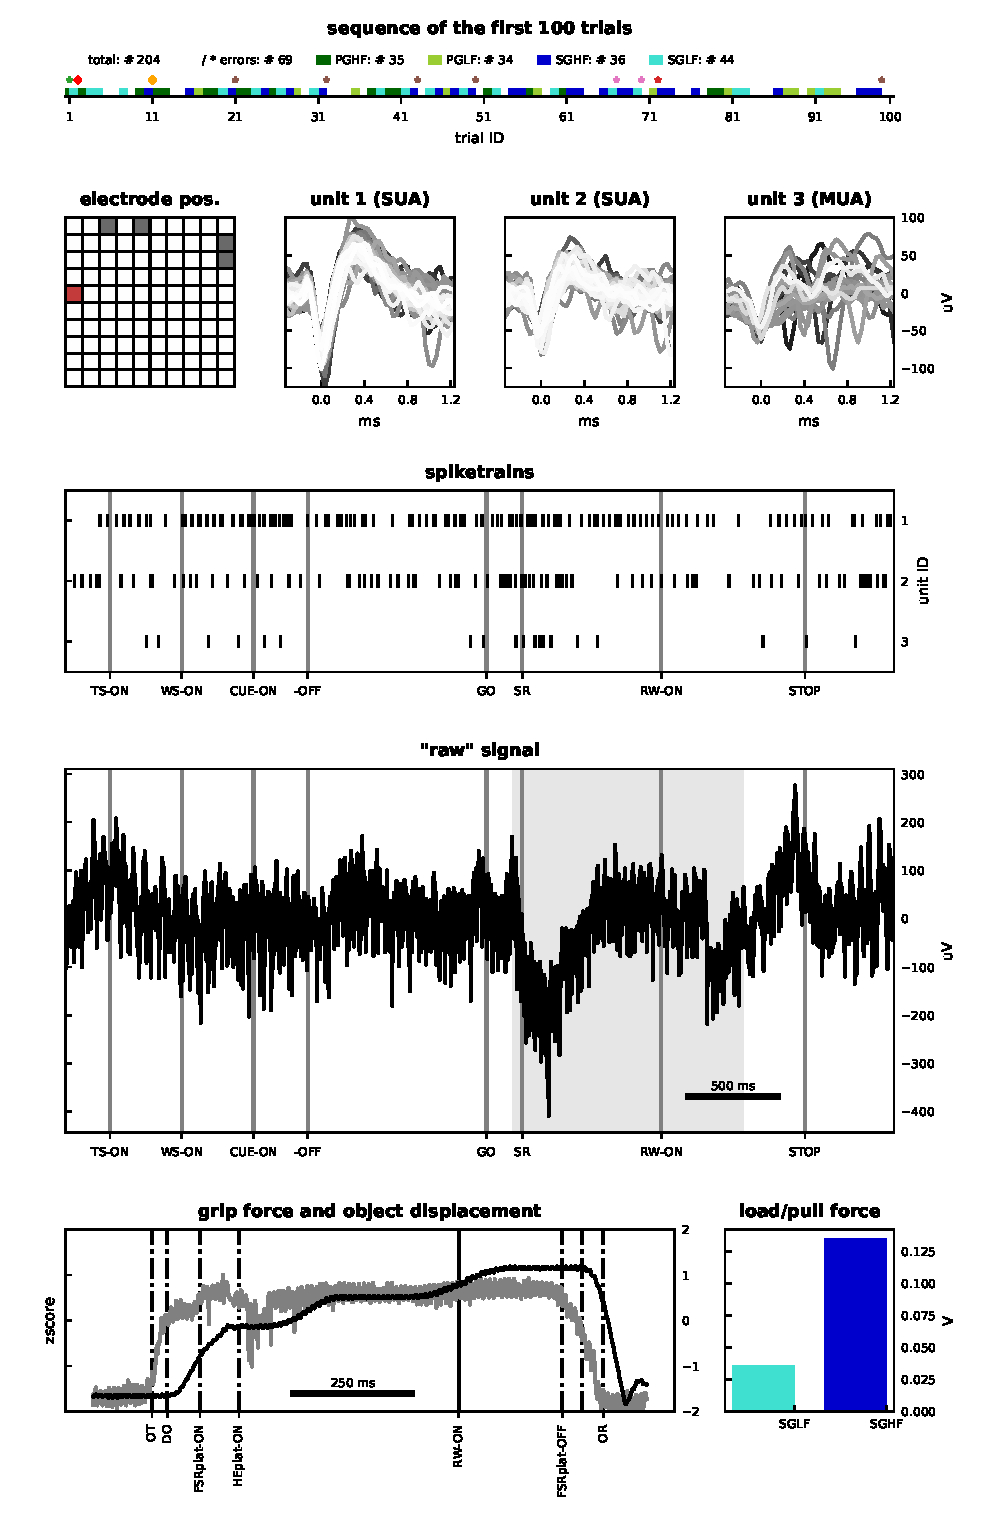
\includegraphics[width=0.8\textwidth]{./figures/scidata_figures/data_overview_1_L}
 \caption[Overview of data types contained in l101210-001]{Overview of data types contained in l101210-001. The figure displays the different data types contained in the selected dataset of monkey L. Top panel: sequence of the first 100 trials (for trial types and errors see color in legend) and the total number of trials (see \# for correct, error, trial types in legend); the red diamond marks the selected trial (trial ID: 2) for panels below; the orange diamond marks an additional trial selected to demonstrate load/pull force differences between the averaged load force signals in the bottom right panel. Asterisks indicate error trials (black asterisks: grip errors). Second row, left panel: position of selected electrode (in red) for the data plots (electrode ID: 71). Second row, remaining panels: waveforms of three units from the selected electrode. Third row: spike trains of displayed units for the selected trial. Forth row: raw signal for the selected trial; gray shaded area marks the time window corresponding to the bottom left panel. Bottom left panel: grip force (gray) and object displacement (black) signals for the selected trial. Bottom right panel: averaged load/pull force signals for the duration of the plateau of the grip force signal for the selected LF and HF trial. Important trial events are indicated as vertical lines in the corresponding data plots.}
 \label{fig:overview_data_l_1}
\end{figure}

\begin{figure}
 \includegraphics[width=\textwidth]{./figures/scidata_figures/data_overview_2_L}
 \caption[Overview of raw signal and spike data of monkey L (l101210-001)]{Overview of raw signal and spike data of monkey L (l101210-001). Left panels: Raw signal (top) and spike data of unit IDs 1 on each given electrode (bottom) for a single trial (trial ID: 2) across a selection of electrodes. Right panels: Raw signal (top) and spike data from single unit ID 1 (bottom) across selected correctly performed trials on one electrode (electrode ID: 3). Trial events (TS-ON, WS-ON, CUE-ON, CUE-OFF, GO-ON, and RW-ON) are indicated as colored vertical lines in each plot. Trial types of selected trials in upper right panels are indicated as color (SGHF: dark blue; SGLF: cyan; PGHF: dark green; PGLF: light green)}
 \label{fig:overview_data_l_2}
\end{figure}

\begin{figure}
 \centering
 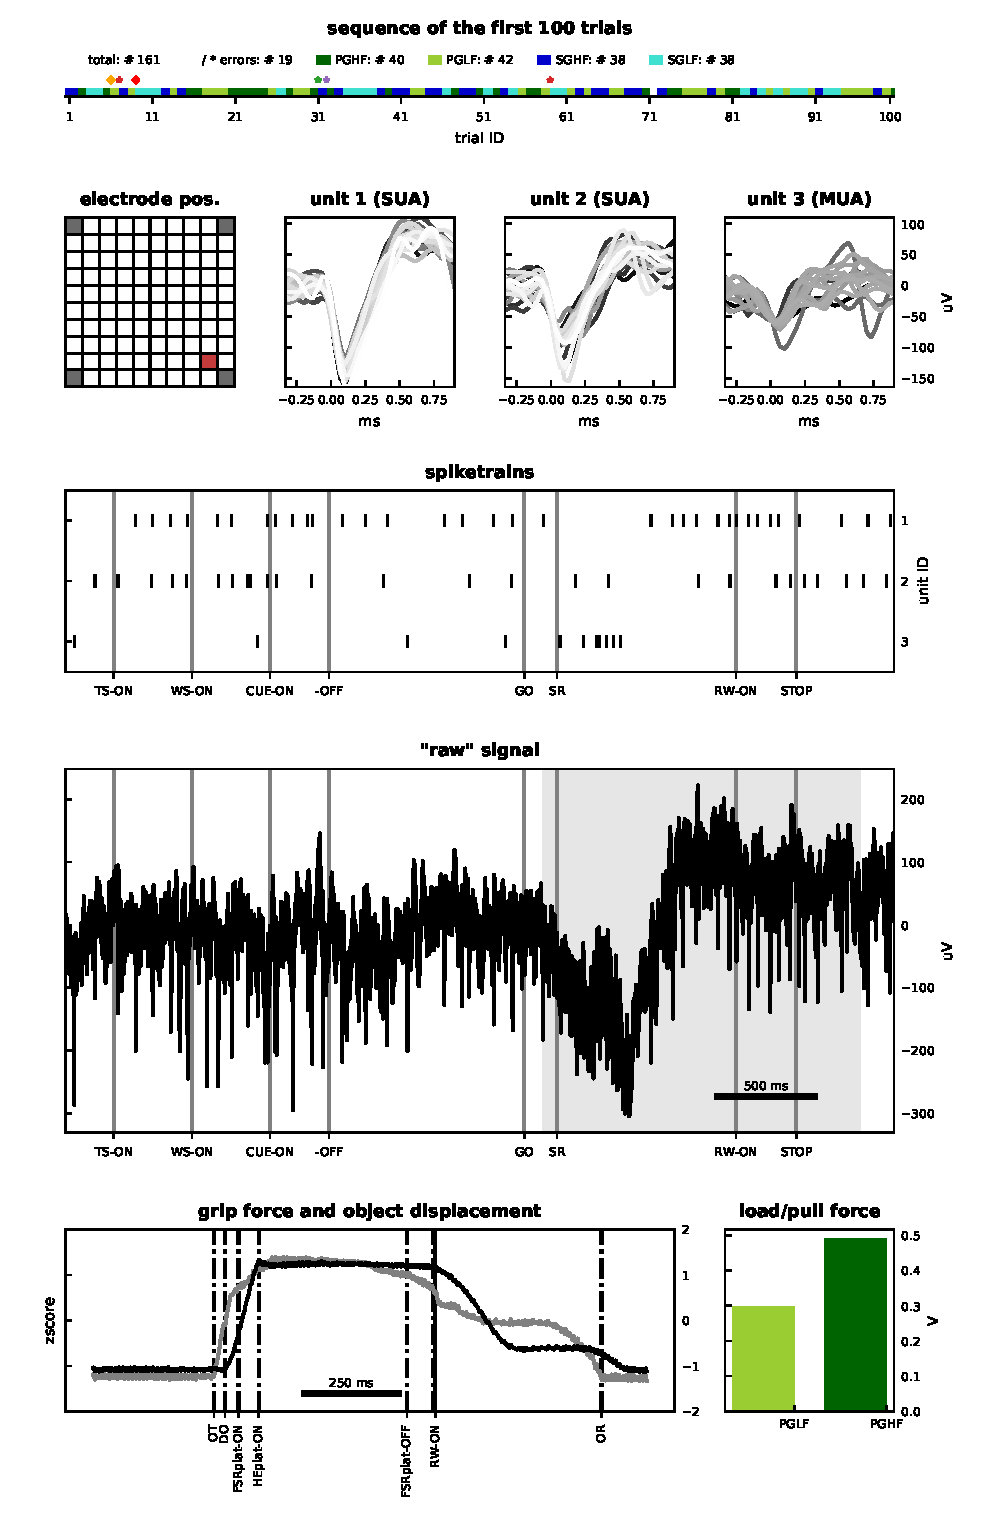
\includegraphics[width=0.8\textwidth]{./figures/scidata_figures/data_overview_1_N}
 \caption[Overview of data types contained in i140703-001]{Overview of data types contained in i140703-001. The figure displays the different data types contained in the selected dataset of monkey N. Top panel: sequence of the first 100 trials (for trial types and errors see color in legend) and the total number of trials (see \# for correct, error, trial types in legend); the red diamond marks the selected trial (trial ID: 9) for panels below; the orange diamond marks an additional trial selected to demonstrate load/pull force differences between the averaged load force signals in the bottom right panel. Asterisks indicate error trials (black asterisks: grip errors). Second row, left panel: position of selected electrode (in red) for the data plots (electrode ID: 63). Second row, remaining panels: waveforms of three units from the selected electrode. Third row: spike trains of displayed units for the selected trial. Forth row panel: raw signal for the selected trial; gray shaded area marks the time window corresponding to the bottom left panel. Bottom left panel: grip force (gray) and object displacement (black) signals for the selected trial. Bottom right panel: averaged load/pull force signals for the duration of the plateau of the grip force signal for the selected LF and HF trial. Important trial events are indicated as vertical lines in the corresponding data plots.}
 \label{fig:overview_data_n_1}
\end{figure}

\begin{figure}
 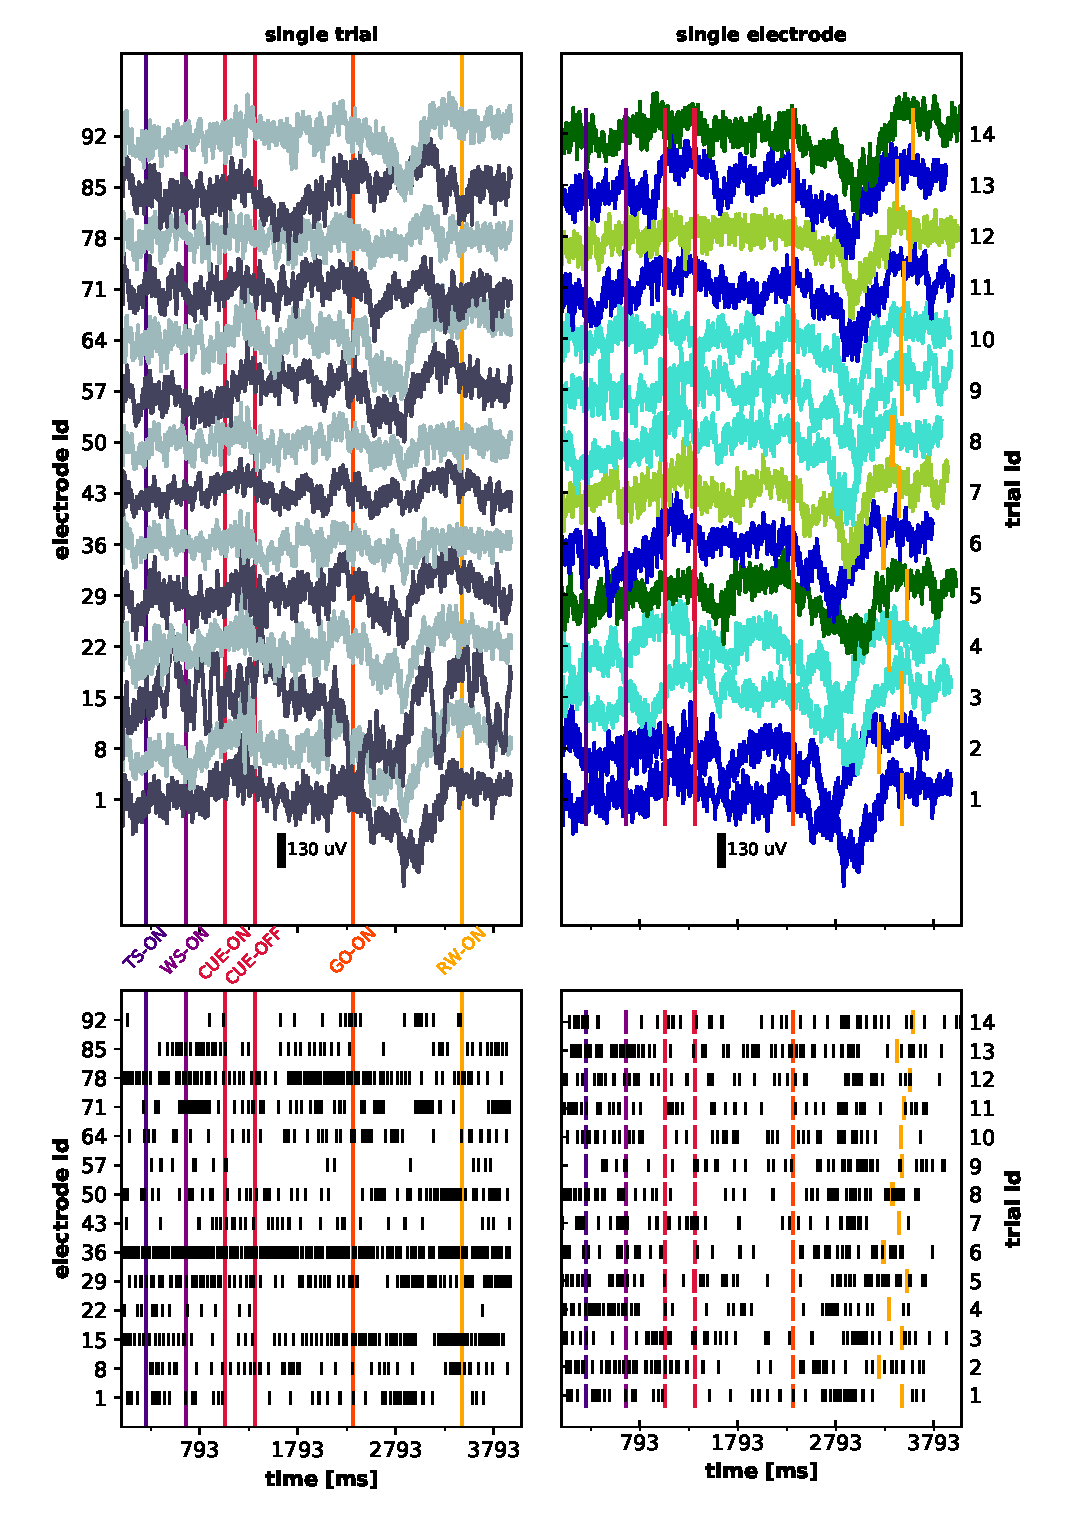
\includegraphics[width=\textwidth]{./figures/scidata_figures/data_overview_2_N}
 \caption[Overview of LFP and spike data of monkey N (i140703-001)]{Overview of LFP and spike data of monkey N (i140703-001). Left panels: LFP data (top) and spike data of unit IDs 1 on each given electrode (bottom) for a single trial (trial ID: 1) across a selection of electrodes. Right panels: LFP data (top) and spike data from single unit ID 1 (bottom) across selected correctly performed trials on one electrode (electrode ID: 1). Trial events (TS-ON, WS-ON,CUE-ON, CUE-OFF, GO-ON, and RW-ON) are indicated as colored vertical lines in each plot. Trial types of selected trials in upper right panels are indicated as color (SGHF: dark blue; SGLF: cyan; PGHF: dark green; PGLF: light green).}
 \label{fig:overview_data_n_2}
\end{figure}


Overview of recording days of the published datasets. For both monkeys, we chose to publish the first dataset (rec*-001) of the recording day. For details on the published datasets see \cref{tab:scidata_data_overview}.

The dataset l101210-001 from monkey L is the first out of 9 recording sessions conducted on Friday, December 10, 2010, while the dataset i140703-001 from monkey N is the first out of only 3 recording sessions conducted on Thursday, July 3, 2014. Both datasets were recorded in the late morning. The following recording day went on for nearly one hour and a half for monkey L, and one hour for monkey N. Although the recording from monkey N lasted with 16:43 min several minutes longer than the recording from monkey L with only 11:49 min, monkey L executed 204 trials, while monkey N only performed 160 trials in total. However, monkey L performed only ~70\% of all trials correctly, whereas monkey N successfully completed ~90\% of all trials during the recording (cf. \cref{tab:scidata_data_overview}). Nonetheless, the high percentage of error trials in monkey L are mainly caused by an too early movement onsets reflecting the eagerness, but also the nervousness of the monkey L's character. In contrast to these error types, monkey L used only 12 times the wrong grip compared to monkey N who performed an incorrect grip type 16 times during the recording. 

Overview of trials performed during the published datasets. Of the stated number of error trials, the monkey L and N used the wrong grip type in 12 and 16 trials, respectively. In the remaining error trials the monkeys initiated the movement too early. Trial types were altered randomly in the recordings which led to slightly different trial numbers for the different trial types.

For both monkeys the trial types alternated randomly between trials leading to slightly different numbers of trials with the same trial type in the each dataset (cf. \cref{tab:scidata_data_overview}). 



The quality of the spiking activity in the datasets of both monkeys was high, which allowed us to perform a relatively robust offline spike sorting with high numbers of single unit activity (SUA) distributed over all electrodes of the array (for details see \cref{tab:datafiles_unitactivity}). For details on how the offline sorting was performed and checked please have a look at \cref{sec:offline_spike_sorting} and \cref{sec:spike_data_quality}. 

\subsection{Information on metadata framework}
\label{sec:scidata_metadat_framework}

 All metadata information about the experiment, the subject, the setup, the settings, the processing of the data etc were originally distributed over several source files, but were collected offline in one metadata file per recording using the \software{odML} metadata framework. This \software{odML} framework was first introduced by \citet{Grewe_2011} and is a supported metadata management project of the G-Node (http://www.g-node.org/projects/odml). \software{odML} files are machine readable and can be used via application programming interfaces (APIs) in Java (https://github.com/G-Node/odml-java-lib), Python (https://github.com/G-Node/python-odml) and Matlab (https://github.com/G-Node/matlab-odml). Moreover, \software{odML} files are human readable and can be screened best by either using the \software{odML} Editor which is part of the \software{odML} Python API, or using a browser via a metadata stylesheet available as download on the G-Node project website. For details on how to manage metadata for such a complex experiment using the \software{odML} framework please have a look at \citet{Zehl_2016}. This reference also includes tutorial like code examples on how to use \software{odML} files in Python and Matlab (see main article as well as supplementary material).

\section{Technical Validation}

In addition to the above described preprocessing steps that needed to be performed to gain more content of the raw data, some technical validations of the data also had to be conducted. These technical validations include the correction of the irregular alignment data files of the Cerebus DAQ system and a general quality assessment of the data. In order to validate the quality of the recording, a series of algorithms were applied to the data. On the one hand the quality of the LFP signals was assessed per electrode and per trial by evaluating the variance of the corresponding signal in multiple frequency bands. On the other hand the quality of the offline sorted single units (\cref{sec:offline_spike_sorting}) was determined by a signal-to-noise measure. In addition, noise artifacts occurring simultaneously in the recorded spiking activity were detected and marked. In the following, we explain these technical validation steps in detail.

\subsection{Correction of data alignment}

The ns6 file starts always 82 samples later than ns5, ns2 and nev files. This miss-alignment is caused by an error in the Blackrock recording software. However, this shift is correctly recorded in the ns6 file, and therefore will be automatically corrected in the generic \software{Neo} loading routine (cf., BlackrockIO in \cref{sec:usage} below). In addition, due to the online filter procedure, the LFP signals in the ns2 file are delayed by approximately 3.6 ms with respect to the time stamps in the nev file and the analog signal of the ns6 file. This offset was heuristically determined, documented in the metadata file, and can be automatically corrected for by the experiment-specific loading routine (cf., ReachGraspIO in \cref{sec:usage} below). Note that the time stamps of the spike times provided in the nev file correspond to start of the waveform and not to the time point of threshold crossing.

\subsection{Quality assessment}

The occurrence of noise in electrophysiological recordings is to a certain degree unavoidable and therefore needs to be carefully examined. It depends to a large extent on the quality of the headstage used to record the neurophysiological data. In our data, two different types of headstages were used for the two monkeys - the Samtec-CerePort headstage (monkey L) and the Patient Cable (monkey N). The former is much more sensitive to noise than the latter. The type of noise, its cause and appearance in the data is quite variable. Depending on the direct influence of the different types of noise on subsequent analysis methods, one needs to balance the corresponding data rejection between being very permissive and very conservative. For this reason, it is wise not remove or delete data of bad quality, but instead mark them with the judgment of a corresponding quality assessment procedure. For the here published datasets, we provide the results of our quality assessment of the electrodes, trials and spiking units along with the analysis parameters of the used procedure in the \software{odML} metadata files for each recording. The reach-to-grasp IO integrates this information by annotating the corresponding data objects in Neo. This approach not only allows the user to finally decide which data to reject for an analysis, but also provides the opportunity to provide different quality assessments of the same electrode, trial and unit at the same time. This is helpful if one considers that certain types of noise can differently contaminate signals in different frequency bands. For the here published datasets, the quality of the recorded signals was therefore separately tested for the sorted spike data and different frequency bands of the LFP data. The used corresponding procedures are described in detail below. 

\subsection{LFP data quality}

The LFP data were examined for noise in three broad frequency bands excluding the 50Hz European line noise (low: 3Hz - 10Hz, middle: 12Hz - 40Hz, high: 60Hz - 250Hz) in each session individually. The goal of the quality assessment was, first, to detect channels with a noisy signal throughout the session and, second, to detect noisy trials in the remaining “clean” channels. To do so, the analog signals of each electrode were first z-scored and filtered in the three frequency bands (low, middle, and high) using a Butterworth filter (of order 2, 3, and 4, respectively). For each frequency band the quality assessment analysis was carried out separately. The detection of noisy electrodes was performed in three steps: 

step 1 The variance of the filtered analog signal of each electrode was calculated over the complete session. 

step 2 Out of the 96 resulting variance values, outliers were identified as those values outside a user-defined range. The range was defined as follows: (i) values between a lower (e.g., 25th) and an upper (e.g., 75th) percentile (L and U), (ii) the range of acceptable values was defined by $L-w\cdot(U-L),U+w\cdot(U-L)$,where w is a user-defined whisker coefficient (e.g., w=3). 

step 3 The analog signals classified as outliers in step 2 were visually controlled by comparing them to the analog signal of an electrode with a typical variance value. If the results were either too conservative or too permissive, the detection procedure was repeated by manually adapting the chosen parameters (L, U, and w), correspondingly. 

The electrode IDs of the final outliers as well as the parameters chosen for their detection were saved in the \software{odML} metadata file of the corresponding recording and marked as noisy for the tested frequency band. 

For the remaining non-noisy electrodes, an analogous procedure was carried out afterwards to detect noisy trials. The procedure differed in one respect: the variance of the filtered analog signal was calculated for each trial on each electrode separately. At the end, the trial IDs of the identified outliers were pooled and marked as noisy for the tested frequency band on all electrodes. The marked trial IDs were saved in the \software{odML} metadata file of the corresponding recording together with the chosen analysis parameters for their detection. Note again that with this procedure a trial is marked as noisy on all electrodes as soon as it is classified as noisy on one electrode.

\subsection{Spike data quality}
\label{sec:spike_data_quality}

To test and judge the quality of the spike data, the results of the offline spike sorting were controlled first, for the signal-to-noise ratio (SNR) from the waveforms of the identified single units and second, for the occurrence of hyper-synchronous event artifacts.

1. To calculate the SNR for each identified unit in the sorting results a method introduced by \citet{Hatsopoulos_2004} was used. The SNR was defined as the amplitude (A, trough-to-peak) of the mean waveform ($<w>$) divided by twice the standard deviation of the waveform noise ($SD_{noise}$) of the defined unit (u): $SNR_{u}=A_{<w>}/SD_{noise}\cdot2$,where $SD_{noise}$ was computed by averaging the standard deviations (SDs) obtained from each sample point across the original waveforms (SD of the waveform noise adapted from \citet{Nordhausen_1996,  Suner_2005}. For all identified single units in the datasets published here, the determined SNRs ranged between $1.5$ and $12$. Corresponding to \citet{Suner_2005} the quality of the spike sorting of an identified unit is good if the SNR is above 4, is fair if the SNR ranges between 2 and 4, and is poor if the SNR ranges between 1 and 2. Units with an SNR below 1 are not considered as signals. For a conservative analysis of the spike datasets, we recommend to use only single units with a SNR of 2.5 or higher, which was our choice in e.g. \citet{Torre_2016}. The results of the SNR analysis of the performed spike sorting were saved in the \software{odML} metadata file of the corresponding recording and units were annotated accordingly. 

2. \todo{Check with Emiliano(s papers). Synchrofact detection based only on SUA and not on all spikes?}Since correlation analysis of spike data is very sensitive to cross-electrode artifacts which would produce unwanted false positive results, we controlled the sorted spike data on their original time resolution ($\delta=1/30ms$) for potential occurrence of hyper-synchronous event artifacts. For this, we computed the population histogram, i.e. the sum of the spikes across all sorted single units in the dataset in bins of $\delta=1/30ms$ (sampling resolution of the data), and detected if there were entries $\ge2$. To our surprise these hyper-synchronous spikes, which are likely to be attributed to cross-channel noise, survived the spike sorting including the cross-channel artifact removal by the Plexon Spike sorter. We indeed detected these spike artifacts during a preliminary analysis of a previous study \citep{Torre_2016}. The number of single units participating in these events ranged from 2 to over 30 and a statistical analysis showed that the frequency of their occurrence largely exceeded the expected value considering the observed population firing rate. Furthermore, a $\delta$-binned time histogram of the population spiking activity triggered around the occurrence times of the hyper-synchronous events revealed also increased spiking activity in the preceding or following bin of the event. For a conservative analysis of the spike datasets, we recommend to treat the spikes participating in a hyper-synchronous event as well as the spikes occurring within a short time interval around this event ($\scriptstyle \pm\delta$) as artifacts of unknown origin and to remove them subsequently before performing any analysis of the spike data.

In \citet{Torre_2016} we combined both quality assessments of the spike data and only considered spikes with a SNR>2.5 and additionally removed all hyper-synchronous events with $\ge2$ spikes. 

\section{Usage Notes}
\label{sec:usage}

In the following, we describe how the provided data files can be practically used in a data analysis scenario. To this end, we first briefly present the open source software libraries we recommend to use in order to access data and metadata using the Python programming language. We also demonstrate how to merge data and metadata in a common representation that facilitates data handling and analysis. Finally, we present an example program that produces a visualization of the most important data items contained in the files, and can be used as a template script for accessing the provided data. All software discussed below is provided in the code subfolder of the provided datasets, and links to the code repositories are listed in \cref{sec:code_availability}.

As outlined above, the datasets are stored in two types of files. The primary data, and the spike sorted data, are provided in the data format (in particular, the nev, ns5 and ns6 format) specified by Blackrock Microsystems, the manufacturer of the recording hardware. Second, metadata are provided as one file in the \software{odML} format \citep{Grewe_2011}. While data and metadata are provided in documented file formats (see http://blackrockmicro.com/ and http://www.g-node.org/projects/odml, respectively), the mere knowledge of the highly complex internal structure of the files is insufficient to practically make use of their content. In particular, implementations of corresponding loading routines performed from scratch by individual researchers are likely to be incoherent and error-prone. Thus, in the following we will use two community supported open-source libraries to separately load primary data and metadata into a generic, well-defined data representation. 

We chose the data object model provided by the open-source \software{Neo} library (\cref{sec:neo}) \citep{Garcia_2014} as the primary representation of the datasets. \software{Neo} provides a hierarchical data structure composed of Python objects that aim to represent electrophysiological data in a generic manner. In addition, \software{Neo} provides a number I/Os that enable the user to read from (and in part, write to) a large number of open and vendor-specific file formats. In particular, \software{Neo} provides an I/O module for the file format used by Blackrock Microsystems (class BlackrockIO in file neo.io.blackrockio.py). The output of this I/O is a \software{Neo} data structure that is a faithful representation of the contents of the primary data files. For detailed information on the structure of the \software{Neo} data object model, please consult the online documentation (http://neo.readthedocs.io/en/latest/index.html).

Here, we briefly summarize the output of the reach-to-grasp datasets obtained when calling the I/O. The \code{read\_block} method of an instantiation of the BlackrockIO returns a \software{Neo} Block object as a top level grouping object representing one recording session. In the hierarchy directly below the Block is one single \code{Segment} object spanning the complete continuous recording, and one \code{ChannelIndex} object for each of the 96 electrodes of the Utah Array (\cref{fig:implant_locations}) and each of the 6 sensor signals monitoring the target object manipulation (\cref{sec:experimental_apparatus}). The data from these 102 recording channels is each saved in one \code{AnalogSignal} object. All of these are linked to the \code{Segment} and the respective \code{ChannelIndex} object. Likewise, the spike times (and optionally, the spike waveforms) of each identified unit are saved to a \code{SpikeTrain} object. As for the \code{AnalogSignal} objects, these are linked to the \code{Segment}, and to the \code{ChannelIndex} object via a Unit object. Finally, all digital events are saved into a single \code{Event} object that lists their time of occurrences and the corresponding event IDs. Additional information from the file is provided as annotations on each individual \software{Neo} object (accessible via the annotation property of the object), in particular as annotations to the top level Block object. Note, that although this generic I/O can be used to access the raw data records, no interpretation of the file contents is given. For example, digital events are not interpreted as behavioral events, but only given as the raw numeric codes shown in \cref{fig:scidata_setup_overview}. 

In order to access the metadata stored in the \software{odML} file, we use the corresponding library API python-\software{odML} described in \citet{Grewe_2011}. In short, \software{odML} files store metadata in form of hierarchically structured key-value pairs. The \software{odML} files accompanying the provided datasets contain extensive metadata grouped into different sections describing different aspects of the experiment. A tutorial on how to work with the \software{odML} library can be found in the online documentation shipped with the library (https://g-node.github.io/python-odml/), and a more detailed description of how to manage metadata by example of the \software{odML} framework can be found in \citet{Zehl_2016}. In short, the library supports to read the content of an \software{odML} file, provides an API to navigate through the hierarchical structure, and to extract metadata of interest from the key-value pairs. Thus, the python-\software{odML} library provides a standardized way to access stored metadata records. 

As a next step, we combine the primary data and metadata in a manner that is specific to this experiment and aids the analysis process. To this end, the relevant metadata that were extracted from the \software{odML} are attached as annotations to data objects in the hierarchical \software{Neo} structure. For example, metadata information for a particular single unit originating from the spike sorting process may be attached to the \software{Neo} objects representing the sorted spike data of that unit. The task of combining the primary data and metadata is performed by a custom-written Python class named ReachGraspIO that is derived as child class from Neo's BlackrockIO class. For a full documentation of the input arguments, methods, and outputs of this class, please refer to the class documentation in reachgraspio.py. In short, invoking the \code{read\_block} method of the ReachGraspIO performs the following steps under the hood: (i) read the primary data using the \code{read\_block} method of the parent class (BlackrockIO) as described above, (ii) read the metadata using the python-\software{odML} library, (iii) interpret event data based on the digital events (e.g., detect trial start or reward), and (iv) add relevant metadata to the \software{Neo} data object using the annotation mechanism. Thus, the \software{Neo} Block object returned by the ReachGraspIO contains extensive information attached as annotations of the individual \software{Neo} objects, in particular, about whether a \code{SpikeTrain} is classified as SUA or MUA, about the spatial positioning of electrodes, or about the identities of electrodes that should be rejected. A full list of these metadata annotations can be found in the documentation of the \code{read\_block} method in the file reachgraspio.py.

In summary, for practical purposes, the resulting data structure of the ReachGraspIO hosts a complete representation of the data and a synthesis of the metadata relevant for analysis. This representation may be saved to disk in a standardized container format (e.g., .mat or HDF5), such that the exact same data and metadata context can also be accessed from other programming languages. For illustration, we provide the data object in the Matlab file format (.mat) in the folder datasets\_matlab, containing Matlab structs resembling the Python \software{Neo} objects.

In the following we demonstrate how to use the ReachGraspIO in practice in order to load and visualize the datasets. We follow the file example.py, which is contained as part of the code included with the published datasets. The goal of this program is to create a figure showing the raw signal, LFP, spikes (time stamps and waveforms), and events in a time window (referred to as analysis epoch) around TS-ON of trial 1 for electrode ID 62. 

In a first step, we load the data using the ReachGraspIO. Considering that only for monkey N an online filtered version of the LFP data is available in the ns2 file, in the following we calculate offline an LFP signal from all raw signals contained in the ns5 or ns6 files using a non-causal low-pass Butterworth filter implemented in the Electrophysiology Analysis Toolkit (Elephant; http://neuralensemble.org/elephant/), which provides analysis capabilities for data stored in the \software{Neo} representation. The parameters of this filter are chosen identical to those of the causal filter for the LFP recorded online in monkey N (\cref{sec:neural_recording_platform}).

In a subsequent step, we extract all TS-ON events in correctly performed trials. To this end, we use the function get\_events() contained in the utility module neo\_utils.py. The function extracts a list of events contained in one \code{Event} object of the loaded \software{Neo} \code{Block} given the filter criteria specified by the parameter event\_prop. In our example, the used filter criteria select all events from the \code{Event} object “TrialEvents” with a trial\_event\_labels annotation set to TS-ON, and a performance\_in\_trial annotation indicating a correct trial.

In a next step, we create \code{Epoch} objects representing analysis epochs around the extracted TS-ON events. To this end, we use add\_epochs() also contained in the utility module neo\_utils.py. The function excepts the previously extracted TS-ON events as trigger, and defines epochs of a given duration around this trigger. The resulting \code{Epoch} object is called “analysis\_epochs”. 

Next, we cut the data according to the analysis epochs and align the cutouts in time. This operation is performed by cut\_segment\_by\_epoch, which returns a list of \code{Segment} objects, each containing data of one analysis epoch. The \code{Segment}s are annotated by the corresponding annotations of the \software{Neo} \code{Epoch}. In addition, the list of \code{Segment} objects is grouped in a new \software{Neo} \code{Block}, named “data\_cut\_to\_analysis\_epochs”. This representation now enables the analysis of the data across trials in the defined analysis epochs. 

In our example, we show how to create a plot of the data of the analysis epoch in one behavioral trial on the selected electrode. To select the \software{Neo} \code{Segment} corresponding to the first correct behavioral trial from the \code{Block} of the cut data obtained in the previous step, we apply the \software{Neo} filter() function. 

From the selected \code{Segment}, LFP data and raw signals can be obtained via the \code{AnalogSignal} objects referenced by the analogsignals property, while spike trains and corresponding unit waveforms can be extracted from the \code{SpikeTrain} objects referenced by the spike trains property. The remainder of example.py uses the matplotlib library to create a figure of the data.

All data and metadata files as well as the code described above can be found in the data repository at \url{https://web.gin.g-node.org/INT/multielectrode_grasp}. The subdirectory datasets contains all data files and the metadata odML-file for the two provided recording sessions. The subdirectory code contains the files example.py and neo\_utils.py. For further reference and inspiration this subdirectory also contains the Python scripts generating the data figures of this manuscript. Furthermore, the subdirectories to code contain frozen versions of the required libraries (Neo, python-odml) as well as the custom loading routine combining data and metadata (reachgraspio.py). Finally, the datasets\_matlab directory contains the annotated \software{Neo} data object containing all primary data saved in the mat-file format. Updated versions of the code, e.g., adapted to new releases of the \software{Neo} library, can be found at https://github.com/INM-6/reach-to-grasp-data-publication.
}

\section{The metadata structure}
\label{sec:scidata_metadata_structure}
All aggregated metadata for a single recording session are collected in a separate \software{odML} file (\cref{tab:scidata_data_overview}). Within an \software{odML} file, information is organized in a hierarchical fashion, following a schema that was defined and continuously refined during the course of the set up of the metadata processing pipeline. \cref{fig:scidata_l101210odml} shows an exemplary part of the metadata collection of the recording session of monkey L. The \software{odML} files contains the following eight top-level sections: \textit{Project} (general information on the reach-to-grasp project), \textit{Subject} (information on the monkey), \textit{Setup} (details of the experimental apparatus), \textit{Cerebus} (settings of the recording system), \textit{UtahArray} (information on the multi-electrode array including spike sorting results and the corresponding quality assessment), \textit{Headstage} (general settings), \textit{Recording} (task settings, trial definitions with event time stamps and periods), \textit{PreProcessing} (results of LFP quality assessment and general information on the spike sorting procedure).
Each top-level \code{Section} contains a branch structure built from \code{Section}s to logically organize the information about the specific aspect of the experiment. For example, the \textit{Subject} \code{Section} contains nine \code{Properties} (denoted by a folder icon), and multiple \code{Section}s beneath, among them for example a  \textit{Training} \code{Section} and \textit{ArrayImplant} \code{Section} (denoted by a collapsible folder icon in \cref{fig:scidata_l101210odml}). All metadata available describing the training of monkey L are the coach (Thomas Brochier), start and end date of the training period (June 2010 - September 2010) and a comment stating that the training was easy and fast. Larger numbers of metadata are stored for describing the recording array used for the recording. Here, the \code{Section} \textit{UtahArray} contains general information about the hardware (material, dimensions, etc) and detailed information about each electrode is contained in the \textit{Electrode} \code{Section}s. Each electrode \code{Section} contains information about the electrode identity and physical location, the impedance value and offline sorting results for data recorded here (not shown in \cref{fig:scidata_l101210odml}). The metadata collection of monkey N has an analogous structure.

\begin{figure}
 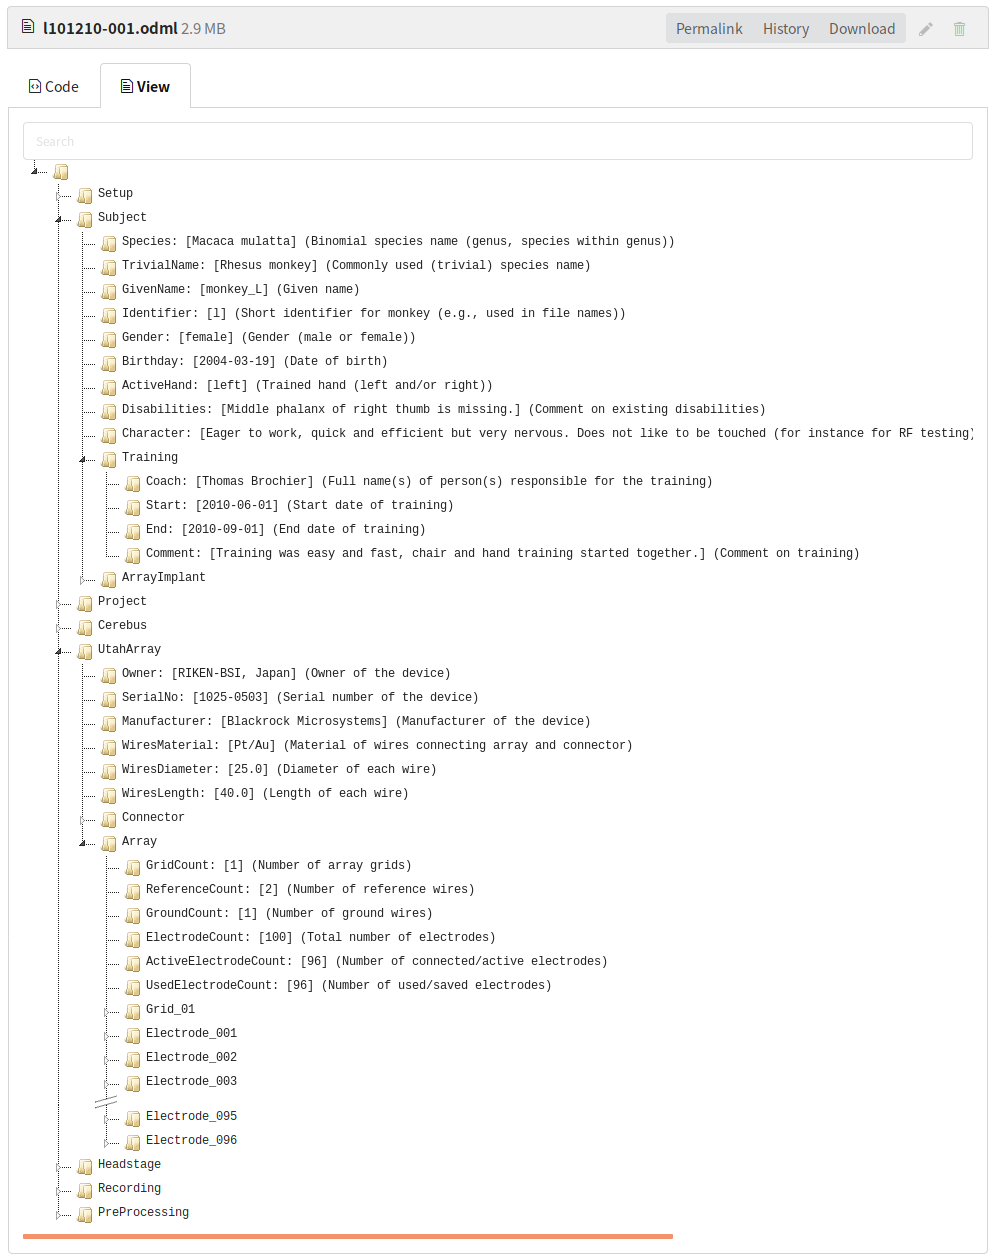
\includegraphics[width=\textwidth]{./figures/scidata_odmltree}
 \caption[Schematic metadata collection of session l101210-001]{Schematic metadata collection of recording session l101210-001 as rendered by the GIN webinterface. \code{Properties} are displayed in the form of \code{<Property Name>: <List of Values> (<Property Description>)}. Individual \code{Section}s are unfolded via user interaction to display the underlying metadata structure. Figure modified from \url{https://gin.g-node.org/INT/multielectrode_grasp/src/master/datasets/l101210-001.odml}.}
 \label{fig:scidata_l101210odml}
\end{figure}

\section{Data and metadata processing pipeline}
\label{sec:r2g_preprocessing_pipeline}
The metadata information as described \cref{sec:scidata_metadata_structure} was aggregated from multiple files and formats into a single file in the \software{odML} format (\cref{sec:scidata_metadat_framework}). This aggregation requires access to, and interpretation of a variety of files and formats, extraction of the corresponding information and integration in the designated location a pre-designed \software{odML} structure. In the pipeline used here (\cref{fig:scidata_metadata_pipeline}), the construction of the \software{odML} structure of a particular recording session is strictly separated from the enrichment of the structure with metadata content. In a first step, an \software{odML} structure with default metadata entries is set up based on multiple Python scripts generating individual branches of the \software{odML} structure. Since the particular structure required for a recording session depends on the specifications of the recording, this process depends to some extend on the metadata to be added (see \cref{fig:scidata_metadata_pipeline}, red arrows). This interdependency requires the metadata to be loaded and partially interpreted prior to the initialization of the structured metadata collection. One example for such a dependency is the existence of spike sorted data after offline spike sorting. Here, first the source files need to be evaluated to extract if the particular session was already sorted to construct the metadata structure accordingly such that it can lateraccommodate potential spike sorting metadata.

After construction of the \software{odML} structure, metadata information is added via a set of custom enrichment functions, i.e., filling available metadata into the structure. This enrichment process is split into different functions that first extract information from the different specialized metadata source file formats and add this data in the \software{odML} structure. In the enrichment process, the location of the target \code{Property} in the structure is implemented by exploiting the filter functionality of \software{odML}. This way, filling the \software{odML} structure requires no detailed information regarding the \software{odML} hierarchy. This provides some degree of flexibility in dealing with variations in the \software{odML} structure, i.e. for different variations of the task or through the continuous improvement of the structure over the course of the experiment. However, given the large number of metadata values to fill, this is computationally more intense than accessing the target location directly via its hierarchy path. Finally, after building and enriching the metadata collection the \software{odML} file with more than $1300$ \code{Section}s, $8000$ \code{Properties} and about $10000$ \code{Value}s is saved.

Setting up this pipeline required preparatory work on multiple levels:
A) The manual preparation of the \software{odML} structure in form of \software{odML} templates in dedicated Python scripts. These scripts mostly comprise between $700$ and $1700$ lines of code and contain the generation of all \software{odML} \code{Section}s and \code{Properties} including default \code{Value}s, since \code{odML} version 1.3 used at that time requires a minimum of one \code{Value} per \code{Property} (see \cref{sec:odml_model_revision}). 
B) The preparation of the metadata source files in the required format. This involved manual offline spike sorting using the \software{Plexon} spike sorter to generate a sorted \code{nev} file and spike sorting \code{mat} and text files containing the resulting metadata. For a single recording session this process requires a few working hours of a trained scientist. Additionally, xls sheets following the \software{odMLtables} standard needed to be set up containing information about the recording (sub)session, the monkey and the recording setup. Furthermore a single text file providing the mapping spatial systems of electrode IDs used in the experiment (\code{brain\_aligned\_elids.txt}) and the results of three \software{Matlab} based preprocessing scripts for detection of behavioural events based on continuous signals (\code{even time markers} and \code{load detection}) and the quality checks for continuous signals in multiple frequency ranges and electrodes (\code{rejections}) need to be provided. Most of these metadata source files are recording session specific and need to be generated after the recording was performed. Typically, these files are generated by the experimenter, however due to the time required for this manual step and the amount of available data, not all of this information becomes available immediately, possibly only years after the experiment.
C) The implementation of the central script to generate the resulting \software{odML}  (\cref{fig:scidata_metadata_pipeline} \code{odMLGenerator.py}) by combining the \software{odML} structure from the templates with the content of the metadata sources. Implementation of this script needs detailed knowledge about both aspects of the \software{odML} generation process to be able to combine the two.

\begin{figure}
 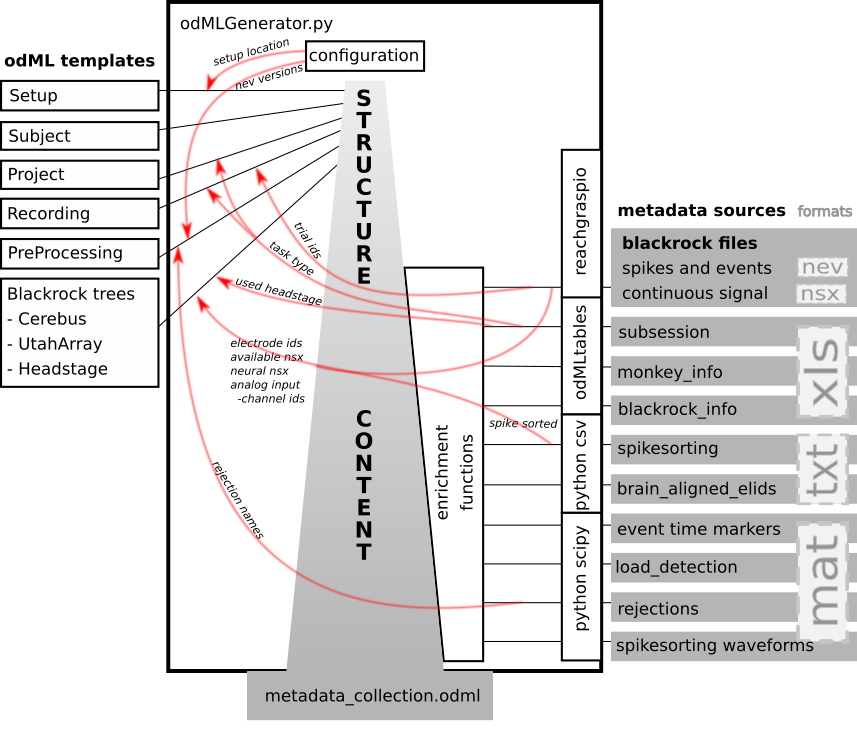
\includegraphics[width=\textwidth]{./figures/scidata_odMLgeneration_diagram}
 \caption[Schematic metadata aggregation pipeline used in \citet{Brochier_2018}]{Schematic metadata aggregation pipeline used in \citet{Brochier_2018}. The \software{odMLGenerator} script (middle box) accesses \code{odML} templates (left box) and metadata source file in different formats (right box). Based on a configuration file, first the structure of the \code{odML} is set up relying on Python scripted \code{odML} templates. In a second step, the structure is enriched with information content from the metadata files. Information from these files is extracted using a variety of different tools (\code{reachgraspio}, \software{odMLtables}, the Python \software{csv} and \software{sicpy} packages) and added to the pre-built \software{odML} structure via custom enrichment functions to generate the final metadata collection. Setting up the \software{odML} structure requires information about the metadata and the configuration (red arrows), which is extracted from the metadata files prior to the building of the \software{odML} structure.}
 \label{fig:scidata_metadata_pipeline}
\end{figure}

\section{Data loading and enrichment with metadata}
\label{sec:data_loading_and_enrichment}
To benefit from a complete metadata collection in the \software{odML} format when loading the original data the metadata should be made easily accessible in combination with the data. This permits the user to access the complete information available during later processing and analysis steps, e.g. for selection of specific trial time periods or recording signals without artifacts. For this, it is essential to combine the information from the metadata collection with the data as the user otherwise needs to switch between different sources and structures for retrieving information. This would introduce additional, unnecessary dependencies in the processing and analysis code.
We provide the \software{ReachGraspIO} Python class which extends the \software{Neo} data structure upon loading with metadata (\cref{sec:usage}). The \software{ReachGraspIO} inherits from the \software{Neo} \code{BlackrockIO} and exploits its functionality to read data from \code{nsX}\footnote{$X \in \{1,2,3,4,5,6\}$} and \code{nev} file formats (\cref{fig:scidata_reachgraspio_diagram}). It returns a \software{Neo} \code{Block} based on the original structure generated by the \software{Neo} \code{BlackrockIO}. The API to interact with the data is therefore the same when using directly the \software{Neo} \code{BlackrockIO} and the \code{ReachGraspIO}. For a detailed description of the \software{Neo} structure and \code{IO}s, see \cref{sec:neo}.

The application programming interface (API) of the \software{ReachGraspIO} is almost identical to the API of the \software{BlackrockIO}. The \software{ReachGraspIO} uses slightly different default parameters, which are adjusted to the datasets generated by the Reach-to-Grasp experiment. The usage of the \code{ReachGraspIO} is demonstrated in an example Python script, which loads the data and visualizes the recording signals at the time point of a trial start (\cref{code:scidata_visualization_1,code:scidata_visualization_2,fig:scidata_visualization}).
Identification and selection of a trial start event in the recording is facilitated by using the \code{ReachGraspIO} instead of the \code{BlackrockIO} directly as the \code{ReachGraspIO} identifies individual trials while loading the data and labels the trial events in a human readable fashion.


\begin{codeenv}
\inputminted[firstline=68, lastline=82, linenos,tabsize=2,breaklines, fontsize=\fontsize{7}{8}\selectfont]{python}{figures/scidata_figures/example.py}
\inputminted[firstline=86, lastline=86, linenos,tabsize=2,breaklines, fontsize=\fontsize{7}{8}\selectfont]{python}{figures/scidata_figures/example.py}
\inputminted[firstline=92, lastline=96, linenos,tabsize=2,breaklines, fontsize=\fontsize{7}{8}\selectfont]{python}{figures/scidata_figures/example.py}
\inputminted[firstline=99, lastline=119, linenos,tabsize=2,breaklines, fontsize=\fontsize{7}{8}\selectfont]{python}{figures/scidata_figures/example.py}
\inputminted[firstline=123, lastline=130, linenos,tabsize=2,breaklines, fontsize=\fontsize{7}{8}\selectfont]{python}{figures/scidata_figures/example.py}
\inputminted[firstline=143, lastline=148, linenos,tabsize=2,breaklines, fontsize=\fontsize{7}{8}\selectfont]{python}{figures/scidata_figures/example.py}
\inputminted[firstline=159, lastline=166, linenos,tabsize=2,breaklines, fontsize=\fontsize{7}{8}\selectfont]{python}{figures/scidata_figures/example.py}
\inputminted[firstline=174, lastline=176, linenos,tabsize=2,breaklines, fontsize=\fontsize{7}{8}\selectfont]{python}{figures/scidata_figures/example.py}
\caption[Example code for loading and processing of published data]{Example code for loading and processing of published data. Metadata annotated data is loaded (line 69-86) and a low pass filtered version of the original signals in generated (line 99-119). Trials are identified and signals are cut into the corresponding segments (line 123-176).  Code extracted from \citet{Brochier_2018}, \url{https://gin.g-node.org/doi/multielectrode_grasp/src/master/code/example.py}}.
\label[codelisting]{code:scidata_visualization_1}
\end{codeenv}

\begin{codeenv}
\inputminted[firstline=195, lastline=253, linenos,tabsize=2,breaklines, fontsize=\fontsize{7}{8}\selectfont]{python}{figures/scidata_figures/example.py}
\caption[Continuation of \cref{code:scidata_visualization_1}: Plotting published data]{Continuation of \cref{code:scidata_visualization_1}. The plotting of the data belonging to the extracted trials for generation of \cref{fig:scidata_visualization}. The figure is initialized and plotting parameters are defined (line 196-199). \code{AnalogSignal}s are visualized (line 201-208) and \code{Spiketrains} are plotted together with the corresponding waveforms (line 213-230). \code{\code{Event}}s are visualized as vertical lines, labelled in human readable way (line 233-242). Finally, the plot is completed and saved in three different formats (line 244-153). Code extracted from \citet{Brochier_2018}, \url{https://gin.g-node.org/doi/multielectrode_grasp/src/master/code/example.py}}.
\label[codelisting]{code:scidata_visualization_2}
\end{codeenv}

\begin{figure}
 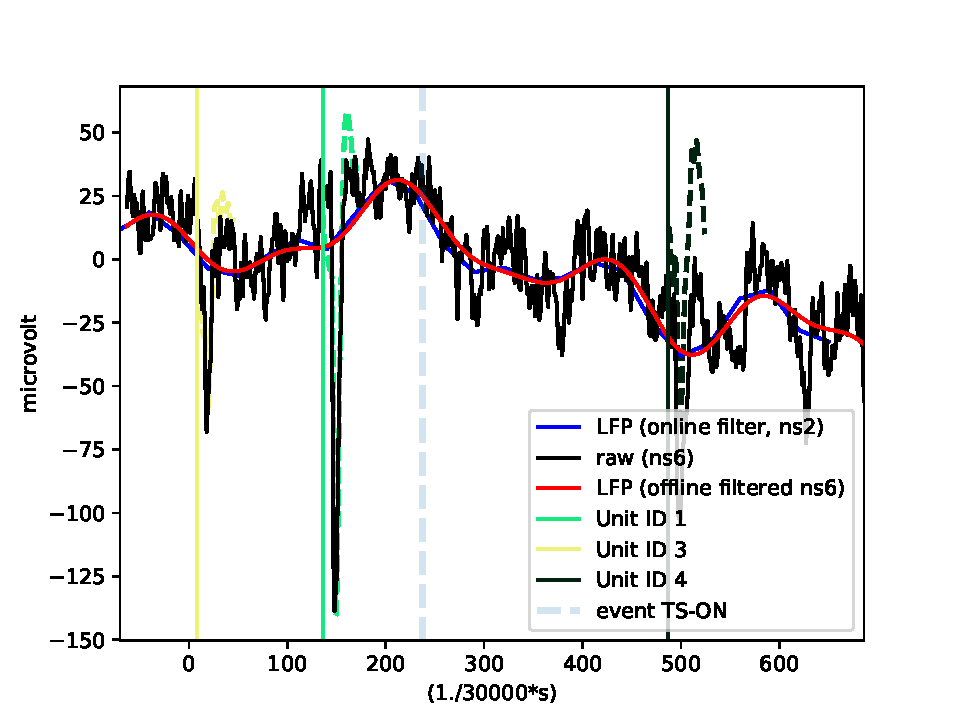
\includegraphics[width=\textwidth]{./figures/scidata_figures/example_plot}
 \caption[Example visualization of the published data]{Example visualization of the published data. The code to generate the figure is shown in \cref{code:scidata_visualization_1,code:scidata_visualization_2}. All recorded data from a single electrode are visualized: the raw, high resolution continuous recording signal (ns6, black), the online filtered continuous recording signal (N's, blue) as well as an offline filtered version based on the raw signal (red). In addition spikes times are marked corresponding to their \software{Unit} assignment and online extracted waveforms are plotted (yellow, green and black traces). Trial events are also visualized (dashed vertical line) and labelled in human readable way (TS-ON, gray).}
 \label{fig:scidata_visualization}
\end{figure}

The \software{ReachGraspIO} extends and annotates the \software{Neo} structure generated by the \software{BlackrockIO} in multiple ways: continuous recording signals are corrected for time shifts introduced by online filters, event times extracted from analog signals are added and a merged representation of events from digital and analog sources is created (\cref{fig:scidata_reachgraspio_diagram}, red box). The first two of these extensions depend on metadata being provided from the metadata collection in \software{odML} format. Additional annotations based on information from the metadata collection are added to most of the \software{Neo} objects (\cref{fig:scidata_reachgraspio_diagram}, gray box). This includes basic metadata describing individual recording traces of \code{AnalogSignal}s, sorting information of \code{Unit}s, general metadata for \code{Segment} and \code{Block} objects, as well as information from the offline trial rejection. If no \software{odML} metadata collection is present, these extension and annotation steps are skipped.
Some of these extension and annotation steps require also additional information, which is available within the \code{ReachGraspIO} as metadata lookup tables. These contain experiment specific code mappings which are essential for the interpretation of the data stored in the original \code{Blackrock} data files. This includes the mapping of bit-coded to human readable notation for events required to define a trial, event codes and equivalence groups, the mode in which the experiment is running (experimental conditions) as well as the performance codes standing for the outcome of a trial attempt (\cref{fig:scidata_reachgraspio_diagram}, green box). These metadata lookup tables are used to translate the bit-based encoding of trial events into human readable versions. If an \code{odML} file is available, trial ids are extracted from there and also annotated. This interpretation of the events is a prerequisite for two further annotation steps: the identification of the task condition, i.e., the task paradigm used in the recording, which again uses a \code{ReachGraspIO} lookup table, as well as the annotation of rejected trials. If digital and analog events are present, these will be merged in to a single \code{\code{Event}} object to simplify the access to all events of recording session (\cref{fig:scidata_reachgraspio_diagram}, 'merge digital \& analog events'). Finally the \code{ReachGraspIO} returns the modified \code{Block} which can be used in further data analysis and visualization scripts (e.g. see \cref{code:scidata_visualization_1,code:scidata_visualization_2}) or in the generation of a metadata collection (see \cref{fig:scidata_metadata_pipeline}).

\begin{figure}
 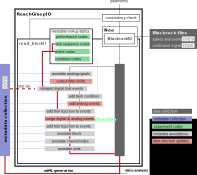
\includegraphics[width=\textwidth]{./figures/scidata_reachgraspio_diagram}
 \caption[Schematic data loading pipeline used in \citet{Brochier_2018}]{Schematic data loading pipeline used in \citet{Brochier_2018}. The \software{ReachGraspIO} (central box) utilizes the \software{BlackrockIO} of \software{Neo} to load the original recording data (top right). In a second step it enriches and extends the data structure returned by the \software{BlackrockIO} containing uninterpreted row data based on additional metadata information from two sources: a metadata collection in \software{odML} format (blue) and ReachGraspIO internal lookup tables (green) containing the essential information required for interpretation the data from the original data files. The extension of the \software{Neo} structure includes correction of time shifts of the recording signals, addition of events which were extracted offline from behavioural signals and the merging of multiple event arrays containing meaningful, human readable events in the trail ('correct filter shifts', 'add analog events' and 'merge digital \& analog events', respectively; red box). The enrichment of the \software{Neo} structure encompasses the addition of numerous annotations (gray box). If no metadata collection is found, these steps are skipped. Finally the extended \software{Neo} structure is returned and can be used for the generation of a metadata collection or further processing and analysis steps. This introduces a circular dependency between the \software{ReachGraspIO} and the metadata collection, as the first one can use the other if present to add trial ids as annotations to the \software{Neo} structure, but also the \software{odML} generation depends on the \software{ReachGraspIO} as essential metadata is annotated based on internal lookup tables (see also \cref{fig:scidata_metadata_pipeline}). Relations contributing to this circular dependency of metadata are marked by red arrows.}
 \label{fig:scidata_reachgraspio_diagram}
\end{figure}




The original pipeline was implemented using Python 2 and \software{odML} version 1.3. The published datasets were updated in 2019 to be compatible with Python 3 and \software{odML} version 1.4. Old versions are still accessible via the published DOI\footnote{10.12751/g-node.f83565, \url{https://gin.g-node.org/doi/multielectrode_grasp}} and the version control system of GIN\footnote{GIN, \url{https://web.gin.g-node.org/}}.

\section{Shortcomings of the \software{odML} generation pipeline}
\label{sec:scidata_shortcomings}
% August 2019: 1974 datasets available at /datasets/marseille/congloue/data/DataGrasp
The presented data publication demonstrates the complexity of the datasets and the efforts required for preparation and release of the data. The complexity of the process is exemplified by the fact that only two of of almost 2000 recording sessions being performed in total with five monkeys were fully described at the time of publication. Here we list reasons we identified that complicate the preparation process:

% additional features in other datasets
\paragraph{Additional features}
\label{sec:additional_features_gaps}
Describing two datasets in a high degree of detail in a manuscript requires 23 pages of descriptor to provide all necessary details. Including additional datasets following the same experimental paradigm would expand the descriptor as additional features observed in the data need to be described. Extending the descriptor to include all peculiarities of all datasets will confuse the reader therefore make the dataset less easily reusable. Moreover, even small additions or changes in the data and metadata processing may result in substantial changes to the pipline design.
An example for additional features which would require explicit description is an additional type of artifact, which is not described in \citet{Brochier_2018} as these two datasets do not exhibit unintended gaps during the recording (\cref{fig:scidata_gaps}). This type of artifact was first described in \citet{Sprenger_2014} and occurs when individual data packets are lost during data recording within the recording hardware. The loss of data packets does not cause an interruption of the recording and is not tracked in the recording file, but the recording files appear intact. Lost data packets can only be detected afterwards by comparing raw continuously recorded data with the corresponding threshold crossing events detected online during recording. After the occurrence of a lost data packet, these two signal are not aligned, as only the continuous signal is affected by lost data packages, and not the threshold crossing events.
For a comprehensive check for gaps during the recording, the \software{odML} generation pipeline would need to be extended in multiple places: Firstly, an additional \code{Section} in the \software{odML} structure would be required to capture the details of potential by a function scanning the original data files. This would require changes in the \software{odML} templates (\cref{fig:scidata_metadata_pipeline}, left box). Secondly, an additional function for gap detection by comparing events to continuous signals needs to be integrated in the \software{odML} generator. This requires extension of the \software{odML} generation code and would potentially increase the run time of the code considerably as the comparison for a full dataset can be compute intense and the \software{odML} generation process is not parallelized. Finally, since the coded detection of gaps can only identify the occurrence of a gap, without reliably characterizing the exact time point or exact extend of the gap, a manual inspection of the data with a detected gap is required after the first run of the \software{odML} generator. To reliably document the results of this manual inspection the integration of the results into the \software{odML} file is mandatory. This could be implemented by the manual generation of a secondary metadata source file, from which the corresponding metadata is extracted during the \software{odML} generation process and included in the metadata collection. However, the suggested procedure requires the execution of the complete \software{odML} generation pipeline twice, once for running the coded detection of gaps and once for integrating potential manually generated additional metadata describing the exact gap time and size. The suggested procedure would therefore more than double the run time of the complete \software{odML} generator for recording sessions with gaps, event though only a small fraction of the metadata was added.

\begin{figure}
 \centering
 \includesvg[width=0.7\textwidth, pretex=\relscale{0.8}]{./figures/scidata_gaps_escus}
 \caption[Origin of gaps in continuous recording data]{Origin of gaps in continuous recording data. Depicted are the recording signals as they are send by the Neural Signal Processor (NSP) ('Real Signal', top) and as they are received by the Central Suite computer (CSC) to be written to disc ('Saved Signal', bottom). For a visualization of the hardware components, see \cref{fig:scidata_setup_overview}. The spike times are extracted from the continuous signals by the NSP and the corresponding time of threshold crossing is attached to each spike. In case of a loss of data during the transfer to the CSC, the spike times are unaffected, only the corresponding spikes of the lost data are not present. For the continuous signal however, the loss of data leads to a concatenation of the remaining samples without considering the original time stamps of the data samples as these are not attached to the data packets (compare sample point marked in red). Therefore the continuous signal is shifted with respect to the extracted spikes starting from the beginning of the gap.}
 \label{fig:scidata_gaps}
\end{figure}


% thorough preparation of all preprocessing steps required
\paragraph{Manual validation}
Preparing the data for data publication requires cross checking of all preprocessing steps (e.g. detection and correction of data packet loss) necessary for that particular set of data. However, in the present scenario, such cross-checks are neither automatized if possible, nor proceduralized. Instead they are performed once a specific dataset is selected for a given analysis, and only specific types of cross-checks relevant for the analysis are typically performed by the researcher.

% variability across datasets not covered by published version
\paragraph{Variability across datasets}
The pipeline for automatic metadata aggregation as presented here has been tested extensively for the two datasets published and the generated files have been manually checked. Running the exact same pipeline on different recording datasets from the same recording has been found to frequently fail, due to slight variations between recording sessions. An intuitive example for this is the set of event codes observed within a recording (\cref{tab:bit_translation}). Here, the interpretation of the observed events codes is performed by the \code{ReachGraspIO} transforming combinations and sequences of bit-encoded events to human readable labels. Due to complex sequences of event codes that may arise, the interpretation of the bit codes in this experiment highly depend on the monkey covering scenarios not encountered for the two published datasets. Extending this to other monkeys and other recording sessions required i) extending the interpreting routine making the code more convolved and less readable and ii) extensive manual validations to ensure the correct interpretation of the bit encoded events.

% availability of source files
\paragraph{Availability of source files and pipeline complexity}
The preparation of source files for the metadata aggregation into a single \software{odML} file is laborious and requires thorough cross checking. Typically, there is no dedicated person responsible for this, but the task is shared between people involved in the experiments. This results in a diffusion of responsibility, as all scientists also have individual projects to care about often focused on a specific subset of the data. For the discussed experiment, not all source file are available for all recording sessions, therefore the generation of an \software{odML} file will not succeed for part of the recording sessions. This mainly affects sessions that are currently not used for analysis due to other quality exclusion criteria. Most importantly, the complexity of the \software{odML} generation leads to a situation where most scientists are not able to properly assist in the curation process.
\newline

In addition to the factors complicating the publication of a high volume of additional datasets from the same experiment as above, there are additional challenges to be taken into account when implementing a metadata aggregation pipeline of the complexity as presented here:

\paragraph{Multiple contributors}
In the case of multiple people involved in the curation process this also requires coordinated activity among all of them. Having individual copies of source files and running the metadata aggregation pipeline using different configurations will lead to various, potentially inconsistent metadata collections. Also the updates of metadata need to be tracked and communicated in a reproducible manner.

\paragraph{Robustness \& Usability}
Special attention also needs to be invested making the execution of the pipeline (or minimally: the result of the execution) available to all collaborators, taking into account different needs and software (version) requirements of scientific projects. The pipeline therefore has to be robust to be run on different machines and different system environments and results need to be compatible with all analysis setups in use. For example for the published datasets accessing the data requires consistent \code{ReachGraspIO} and \software{Neo} versions.

\paragraph{Structure \& Reusability} The presented metadata pipeline separates the generation of the structural templates of the \software{odML} and their enrichment with metadata values. This separation is a good approach during the design of the metadata pipeline, as a general structure first needs to be established before implementing the enrichment. During the production phase of the \software{odML} generation, however, this separation results in a coupling between the two phases, as for the enrichment of the \software{odML} structure knowledge about the structure is required. During the runtime of an experimental series frequently also structural adjustments and extensions to the \software{odML} tree need to be performed as the experimental design was updated or the need to track additional metadata was recognised. The modification and extension of the metadata structure during the production phase always requires changes on both ends of the \software{odML} generation process (structure building \& enrichment), leading to an overly complex procedure to adjust the pipeline which is hard to maintain.
Due to the separation of the structural templates and their enrichment with metadata only the template \software{odML} files are easy to extract from the presented pipeline for application in a different experiment. The enrichment of the structure is built-in the \software{odML} generation pipeline and can not be easily transferred to another metadata pipeline as this is code is specific to the metadata source files.

\paragraph{Linearity}
The presented pipeline for generating a metadata collection relies on the usage of the \code{ReachGraspIO} (\cref{sec:data_loading_and_enrichment}) for a basic interpretation of recorded events using the internal metadata lookup tables. Hard coding metadata processing in this manner is a reasonable approach to make the data quickly usable while the experiment is still under development, but in a stable configuration this introduces cyclic dependencies. In the example presented, the \code{ReachGraspIO} relies on an (optional) \software{odML} file to provide metadata on the one side and on the other side the \software{odML} generation process depends on the usage of the \code{ReachGraspIO} (see \cref{fig:scidata_metadata_pipeline,fig:scidata_reachgraspio_diagram}). This introduces additional dependencies between software versions and metadata and convolutes the data loading from metadata interpretation and annotation aspect.

\paragraph{Portability} The presented metadata pipeline relies on specific versions of software packages, whereas typically in an experimental environment the exact versions used are not necessarily well documented in a rigorous fashion. Therefore executing the pipeline on a different system ,e.g., a high performance cluster, requires expert knowledge and additional effort to satisfy all version dependencies of the pipeline with respect to other software packages.

\paragraph{Consistency} Working with the published data requires multiple compatible files to be present: the original data files, the metadata collection, and multiple software packages including multiple custom codes, in particular the \code{ReachGraspIO} and \software{Neo} in combination with \software{odML}. In other words, a researcher must use the same versions of all of these components as was used during the \software{odML} generation process. The version compatibility between all three aspects is typically only neglectfully documented and needlessly complicates the setup of a system to work with the data. Moreover, it locks the users into versions of libraries that may become outdated over time.



\section{Requirements for Maintainable and Reproducible Metadata Management}
\label{sec:metadata_requirements}
Based on the experience from publishing the two datasets (\cref{sec:scidata_shortcomings}) we identify essential requirements for maintainable and reproducible metadata management pipelines in complex, collaborative projects.

\begin{description}
 \item[R1: Common terminologies] To have a foundation for communication between collaboration partners it is important to agree on common terminologies. Within a scientific discipline, this might be given to a sufficient degree from mutual understanding, but as soon as scientists from multiple backgrounds need to interact, agreeing on common terms is an essential first step. Formalizing this in a documented way in the metadata collection is part of this process and documents the terminology also for future generations of scientists but also within the run-time of a single project.
 \item[R2: Structured machine \& human readable metadata] The metadata collection needs to be programmatically accessible to be used for data annotation and querying. However, metadata also needs to be human readable, for manual checks and scanning of metadata. This becomes of special importance in the context of laboratory notebooks and how automatically generated metadata collections can substitute the manual notebooks in the long term. Finally, if metadata are machine accessible this information can automatically be used during data processing and analysis (e.g. for labelling in data visualization). However this approach only makes sense if the data is additionally human readable, as in the in the long run scientists inspect the processing and analysis results.
 \item[R3: Central data and metadata location] As discussed in \cref{sec:scidata_shortcomings}, in a collaborative environment a systematic organization of metadata is essential. Providing access to data and metadata via a central data storage is a straight forward solution. 
 \item[R4: Version control] To be able to communicate efficiently about data and metadata, version control can assist in collaborative curation, but also in making changes and addition to metadata visible. Using version control the usage of identical data and metadata versions by different scientists can be guaranteed as well as changes in the data and metadata collection can be tracked easily. This permits to track updates and changes on the data and metadata side and documents these.
 \item[R5: Mostly automatic metadata compilation] With the large amount of metadata accumulating it is a high priority to automate metadata aggregation as far as possible. In some cases this is not possible in all cases, e.g. when metadata are only available in hand-written form in laboratory notebooks. This type of metadata however is a very small fraction of metadata and has to be digitized manually in most cases.
 \item[R6: Extendable metadata workflow] As discussed in \cref{sec:scidata_shortcomings} scientific metadata workflows need to be easily extendable to cope with latest analysis requirements and scientific findings.
 \item[R7: Reusability] Scientific workflows should be (partially) reusable for related projects to simplify the setup of similar workflows and save time in implementing these.
 \item[R8: Standardized \& reproducible preprocessing] Standardizing preprocessing steps improves clarity and rigour of the preprocessing tools and contributes to the aspect of Reusability of the workflow. Making the individual preprocessing steps reproducible e.g. by tracking used packages (provenance tracking) and documenting the code version helps making the whole workflow reproducible.
 \item[R9: Easy to access data and metadata for non-experts] Data and metadata should be easy to use by non-experts of the preprocessing pipeline. In the ideal case an out-of-the-box solution can be presented to the user, who can load the data immediately without installing a series of software dependencies. 
 \item[R10: Consistent data and metadata] Data and metadata should always be consistent. This includes the guarantee that,e.g., preprocessing steps performed on the data should also be reflected in the metadata collection. The concept of version control and reproducibility aid the consistency ensurance.
 \item[R11: Open source tools] In as much as possible, the workflow should use open source software tools that provide their source code to the community. This has the advantage of validation of the correct functionality by other users and permits to fix potential errors. For community software projects also code corrections and enhancements can be suggested and will usually be reviewed and integrated into the tool. Open source tools are free of charge and therefore provide a suitable basis for scientific work to be independent of industry.
\end{description}


\subsection{Evaluation of presented metadata pipeline}
\label{sec:r2gpipeline_evaluation}
The pipeline used for metadata aggregation and access in \citet{Brochier_2018} is described in \cref{sec:scidata_metadata_structure}. In \cref{sec:metadata_requirements} we identify a eleven requirements for maintainable and reproducible metadata management. In the following we evaluate the presented pipeline with respect to these requirements. \cref{tab:requirement_check_scidata} summarizes the findings.
\newline

The presented metadata pipeline consists of two main components: the \ \code{odMLGenerator} for integrating the metadata in a single \software{odML} metadata collection and the \code{ReachGraspIO} for data access and integration with metadata. By utilizing \software{odML} for metadata storage the requirement of having common terminologies (\requirement{R1}) is fulfilled on a project level in this pipeline, since \software{odML} requires the specification and definition of terms within the collection which is then shared between collaborators. This approach also guarantees that the metadata collection is machine and human readable (\requirement{R2}), as the \software{odML} file is xml based and provides tools for user friendly visualization (\software{odMLtables} (\cref{sec:metadata}), odML-UI\footnote{\url{https://pypi.org/project/odML-UI/}}, odml\_view\footnote{\url{https://github.com/G-Node/python-odml/blob/master/odml/scripts/odml_view.py}}).

The pipeline itself does not include the automatic storage of data or metadata or related scripts at a central location (\requirement{R3}). However, combining the pipeline manually with a central server or a common data hosting platforms is straightforward as data as well as metadata files are self contained. By using a central data hosting platform which supports version control, like GitHub\footnote{\url{https://github.com/}}, GitLab\footnote{\url{https://about.gitlab.com/}} or GIN\footnote{\url{https://gin.g-node.org/}}, version control can be automatically introduced at the same time (\requirement{R4}). Alternative to using version control in combination with a remote server, a version control system can also be implemented locally, e.g. by using git\footnote{\url{https://git-scm.com/}}, git-annex\footnote{\url{https://git-annex.branchable.com/}} or git-lfs\footnote{\url{https://git-lfs.github.com/}} to version data locally.

The presented metadata pipeline is automated in the sense that it does not require direct manual interaction (\requirement{R5}). However, a fully automated workflow would include automatic initiation of the pipeline upon a change in the source files. This is not the case here, as there is no trigger mechanism included here. Instead, the pipeline is triggered by the user and can be performed selectively on a subset of available files. The latter is bound to lead to a situation where the metadata collection of the complete experiment becomes inconsistent. Possible extensions including this would be the integration of centrally hosted code in combination with a web hook to a continuous integration service like Jenkins\footnote{\url{https://jenkins.io/}}, Travis\footnote{\url{https://travis-ci.org/}} or CircleCI\footnote{\url{https://circleci.com/}}. In this way adding or modifying metadata sources or the code to generate \software{odML} files in a repository would automatically trigger the \software{odML} generation process.

The extendability (\requirement{R6}) of the presented pipeline is limited, as changes in the metadata always require code changes in multiple locations (see \cref{sec:scidata_shortcomings}, 'Additional features', 'Variability across datasets', 'Structure \& Reusability') and dependencies between structure and metadata need to be explicitly implemented in the \code{odML} generation process. This requires expertise knowledge about experiment, its metadata and the metadata pipeline and leads to convoluted code due to the monolithic design of the pipeline.

The separation between building the structure of the \software{odML} document and the enrichment with metadata makes parts of the structural templates usable for other experiments if they contain similar hardware, software or preprocessing components. However, the code for enriching these template structures is highly specific to the non-standardized formats of the metadata source files in this experiments. Therefore the reusability of the presented workflows for other experiments is limited to parts of the structural template of the \software{odML} document and a few generic routines (\requirement{R7}).

The compilation of the \software{odML} document in the presented pipeline is a single Python script that relies on a number of additional Python modules for the aggregation process. No provenance is captured in the process and the final \software{odML} file does not contain any information about its generation process (\requirement{R8}). In particular, this means that for the \software{odML} file it is impossible to match the version of the \code{ReachGraspIO} or the \software{odMLGenerator} and the content can not be verified. Possible extension to the pipeline could be the usage of a provenance tracking tool like Sumatra\footnote{\url{https://pythonhosted.org/Sumatra/}} or explicit tracking of file and package versions used in the pipeline.

For accessing the data in combination with the collected metadata in the \software{odML} format multiple software requirements need to be installed in specific versions: \software{Neo} for providing the data structure, \software{odML} for metadata handling, the experiment specific \code{ReachGraspIO} for combining the two as well as the original data files with a specific version of the \software{odML} file. All of these have version interdependencies, which need to be considered when setting up an analysis based on the published data. In particular, version requirements of the analysis process may conflict with that of the code to access the original data files, e.g. by requiring different \software{Neo} versions. Therefore installation of an analysis pipeline based on the published dataset requires some effort and time and can be demanding for non-experts (\requirement{R9}). Also, this may lead to analysis relying on outdated package versions and not benefiting from bug fixes and upgrades, as dependencies are restricted by the the packages required for initial loading of the data.

In the presented workflow the consistency of data and metadata is not explicitly checked. Especially after the \software{odML} file generation, there is no mechanism to validate the metadata and data (\requirement{R10}). An indirect mechanism to ensure consistency of data and metadata files is to introduce provenance tracking (\requirement{8}) in combination with version control mechanisms (\requirement{R4}).

By using Python for the presented metadata pipeline in combination with the open-source software packages \software{odML}, \software{odMLtables} and \software{Neo} \citet{Brochier_2018} rely strongly on open-source software (\requirement{R11}). Some exceptions are preprocessing steps, which are required to generate the metadata source files, e.g. spike sorting using \software{Plexon} and a custom event detection implemented in \software{Matlab}. Also the recording setup is based on \software{Windows} and closed-source recording software by \code{Blackrock Microsystems}, but in principle alternative open-source projects electrophysiology recordings (open ephys\footnote{\url{http://www.open-ephys.org/}} and spike sorting (e.g. tridesclous\footnote{\url{https://github.com/tridesclous/tridesclous}} exist, but need to be evaluated in the context of this and future projects.


\begin{table}[]
\begin{tabular}{|l|l|}
\hline
Requirement                                          &  \cite{Brochier_2018} \\  \hline
R1: Common terminologies                             &  in project \\ \hline
R2: Structured machine \& human readable metadata    &  yes \\ \hline
R3: Central data and metadata location               &  no \\ \hline
R4: Version control                                  &  no \\ \hline
R5: Mostly automatic metadata compilation            &  manual initialization \\ \hline
R6: Extendable metadata workflow                     &  minimal \\ \hline
R7: Reusability                                      &  partial \\ \hline
R8: Standardized \& reproducible preprocessing       &  no \\ \hline
R9: Easy to access data and metadata for non-experts &  partial \\ \hline
R10: Consistent data and metadata                    &  partial \\ \hline
R11: Open source tools                               &  mostly \\ \hline
\end{tabular}
\caption[Overview of workflow features for \citet{Brochier_2018}]{Overview of workflow features for \citet{Brochier_2018} based on requirements for data and metadata workflows as defined in \cref{sec:scidata_shortcomings}. The presented pipeline fulfills basic criteria regarding common terminology definition and structured and readable metadata and the usage of open source tools. Other criteria are partially or not met.}
\label{tab:requirement_check_scidata}
\end{table}

\clearpage
\chapter[Metadata management]{The basis for reproducible science - metadata management}
\label{sec:metadata}


\todo{Add logo of odMLtables}
\section{Introduction}
\label{sec:Introduction}

In recent years, the workflows involved in conducting and analyzing neurophysiological experiments have become increasingly complex \citep[e.g.][]{Coles_2008, Denker_2016, Brochier_2018}. Several factors contribute to this development. Nowadays, a recording setup is usually comprised of several hardware and software components that are often produced by different companies, or might even be custom made. In addition, due to the technological progress in neuroscience during the last decades the task designs have become more and more sophisticated, as can be observed, for example, when considering experiments mimicking realistic, natural conditions. Neuronal or muscular signals (e.g., eye and arm movements) can be gathered in parallel from multiple optical or electrical recording sites \citep{Nicolelis_2002,Verkhratsky_2006,Obien_2014} together with complex behavioral measures \citep{Jacob_2010,Maldonado_2008,Vargas-Irwin_2010,Schwarz_2014}. Moreover, these signals can be experimentally manipulated in intricate ways, e.g., via multidimensional natural stimuli \citep{Geisler_2008} or sophisticated optical or electrical stimulation methods \citep{Deisseroth_2013,Miyamoto_2015}. As a result, the amount of information required to fully describe all circumstances under which the experiment was conducted and data was recorded, here collectively referred to as ``metadata'', has grown considerably at the same time. Therefore, metadata of neuroscientific studies are increasingly difficult to document and the implementation of specific software solutions to facilitate their management in daily routines involves a lot of time and effort \citep{Zehl_2016}.

The complexity of collecting metadata originates from two factors: Firstly, the growing heterogeneity of setup equipment alone makes it difficult to fully track the exact circumstances under which the primary data were recorded and how the recorded signals were processed along an experimental recording session ("black box" effect, i.e., the difficulty to precisely relate inputs and outputs to the equipment). Secondly, the complexity of the signal types and manipulations using various tools within custom signal processing pipelines increases the effort needed for comprehensive metadata tracking across all parts of the recording system and all processing steps. In particular, the hardware components and software tools employed in these experimental setups typically do not provide a complete account of their metadata and store their output in non-standardized representations that impede gaining insights into the details of the recording process. Nonetheless, collecting and providing metadata of an experiment is a necessary step towards replicable experiments and therefore forms the basis for reproducible research \citep{Tebaykin_2017}. In this regard, metadata have to be human readable in order to give users semantic access to the data, similar to a traditional lab book. However, only standardized, machine-readable metadata can be systematically reproduced during automatized analysis processes, which makes them a crucial ingredient for tracking the data provenance leading to a research publication.

A software approach to manage neuroscientific metadata is the \textit{open metadata Markup Language} (odML) framework \citep{Grewe_2011}. It has been actively developed and extended during the last years to version 1.4, which is considered in the following. The implementation of the \software{odML} format is based on the generic eXtensible Markup Language (XML) and provides an application programming interface (API) for Python and Matlab. It is designed to organize metadata of arbitrary type into a standardized, hierarchically structured format that is both human and machine-readable. With this, it is possible to organize metadata originating from heterogeneous sources in a unified way and record them in an interoperable format. Providing metadata in such a standardized format along with the data files of an experiment facilitates the collaboration process between members of a scientific project, because metadata can be organized and made available to all members in a unified way, thus supporting rigour and reproducibility of data analysis through standardized and formalized access to the available metadata \citep{Zehl_2016}.

\cref{fig:odMLgeneration} shows a generic representation of an example workflow that results in the generation of a metadata collection represented in odML. The starting point are collections of files containing various subsets of the metadata for individual recordings of an experiment (e.g., different recording days). The data in these files are often organized in different formats within a collection, and files and metadata between different collections may differ due to factors such as changes in the experiment. Therefore, it is possible and advisable to construct template structures for the metadata collection to enforce a systematic metadata structuring. However, in practical scenarios often custom scripts are required to populate these templates, e.g., to cover small variations between metadata collections when a certain piece of information is not present for a particular recording. In addition, the metadata collection must be manually enriched by information that is not digitally available in the first place. The outcome of this build process are \software{odML} files for each recording, adhering to a uniform template structure. In a final step, these individual metadata collections may be merged into a single \software{odML} file in order to provide scientists with the ability to perform full metadata queries on the complete experiment. \citet{Zehl_2016} provides a complete account of this workflow including practical examples.

Implementing and applying such a rigorous workflow as described in \cref{fig:odMLgeneration} requires programming skills by the scientist. However, metadata handling is often performed by several experimenters with varying computational expertise. Furthermore, extensive manual editing of the metadata files via the present graphical user interface (GUI) included in the \software{odML} framework tends to be cumbersome for large metadata trees due to their hierarchical, complex organization. While visualization of the hierarchical organization is suited for an overview of the general structure and relation of the metadata, finding or comparing particular values can be difficult if they are distributed in different branches of the hierarchy. Furthermore, editing of distributed entries is laborious, because a hierarchical organization also requires navigation through the tree to access a particular entry. This makes this metadata management tool inefficient to use in an experimental laboratory where often (i) single particular entries need to be modified manually as the experiment progresses, (ii) a batch of similar entries need to be modified coherently as the data processing progresses. The combinations of all these factors results in many experimental laboratories frequently collecting metadata in flat tabular formats independent of an explicit, underlying hierarchical structure, using tools for generation and manipulation of tables that do not require programming expertise, are widely adopted, readily available and familiar to the experimenters.

Thus, for these purposes a flat tabular representation of the metadata appears to be suitable. It has the advantage of providing easier access to, and simpler visualization of, the metadata than a hierarchical format. Tabular representations of hierarchical structures are implemented in a number of generic software tools for \code{xml} representation\footnote{See, e.g., \url{https://www.oxygenxml.com/xml\_editor/xml\_grid\_editor.html} or \url{http://rustemsoft.com/xfox.aspx}}. However, these generic \code{xml} editors do not provide support for using \code{xml} to handle scientific metadata in a concise way.

We developed \software{odMLtables} as a Python package to complement the \software{odML} framework in simplifying working with, and in particular manually editing, the metadata stored in the hierarchical \software{odML} format. \software{odMLtables} facilitates the integration of the \software{odML} framework into the experimental workflow by converting between hierarchical \software{odML} and tabular representations in \code{xls} or \code{csv} format. These tabular formats are easily accessible via commonly known spreadsheet tools (e.g., \textit{Microsoft Excel}, \textit{LibreOffice Calc}) that enable neuroscientists to manually extend or edit the content of an \software{odML} metadata file. More importantly, the \software{odMLtables} package comprises a GUI that guides the user through all functional features of the tool. With this, it also opens access to the \software{odML} framework for scientists with little or no programming experience. All main functionality to interact with metadata files is directly accessible from the \software{odML} GUI since version 1.4.0. The software has benefited from the experiences gained in applying it in collaborative projects involving three different experiments collecting electrophysiological data: (i) cortical activity in macaque performing a visually-guided motor task \citep[e.g.,][]{Denker_2018,Brochier_2018}, (ii) cortical and hippocampal activity in a developmental study in mice \citep[e.g.,][]{Bitzenhofer_2017}, and (iii) cortical activity in a category learning task in gerbils \citep[e.g.,][]{Ohl_2001}.


The embedding of \software{odMLtables} in a real world metadata management workflow is described in \cite{Zehl_2016}, resulting in a published dataset with detailed metadata descriptions in the \software{odML} format  \citep{Brochier_2018}. In both papers the focus resided on the concepts of metadata management and the detailed experiment description, whereas here we complement these studies by a technical tool to implement metadata capture. While the described experiment (an instructed, delayed reach to grasp task with multielectrode recordings from monkey motor cortex) is too complex to present the features and usage of odMLtables, the concepts presented here are abstracted from these studies.

To optimally demonstrate the application of \software{odMLtables} we present seven minimalistic scenarios of practical metadata management using \software{odML} and odMLtables. Together these scenarios form a complete metadata workflow based on an exemplary multi-day experiment as commonly encountered in neurophysiology (cf.~\cref{fig:odMLgeneration}), but also other fields of science where data is aggregated in repetitive acquisition cycles (e.g., multiple days of measurements). Moreover, the scenarios are of sufficiently generic nature to transfer them to other situations where metadata information is collected. The first two scenarios demonstrate the first steps for setting up a new metadata workflow and daily metadata collection. Four scenarios deal with the ongoing metadata validation, enrichment and visualization. The last scenario introduces automation of metadata collection and management using \software{odML} and odMLtables.

In general, \software{odMLtables} facilitates access to sophisticated metadata management software \software{odML} for non-programmers and with that optimizes routine manual metadata acquisitions in any laboratory workflow. In addition, \software{odMLtables} can be used to create visually enhanced tabular overviews of complete or filtered metadata from any hierarchically structured \software{odML} files. For a scripted metadata approach a Python interface permits also programmers to benefit from \software{odMLtables} features.

\begin{figure}[!ht]
\begin{center}
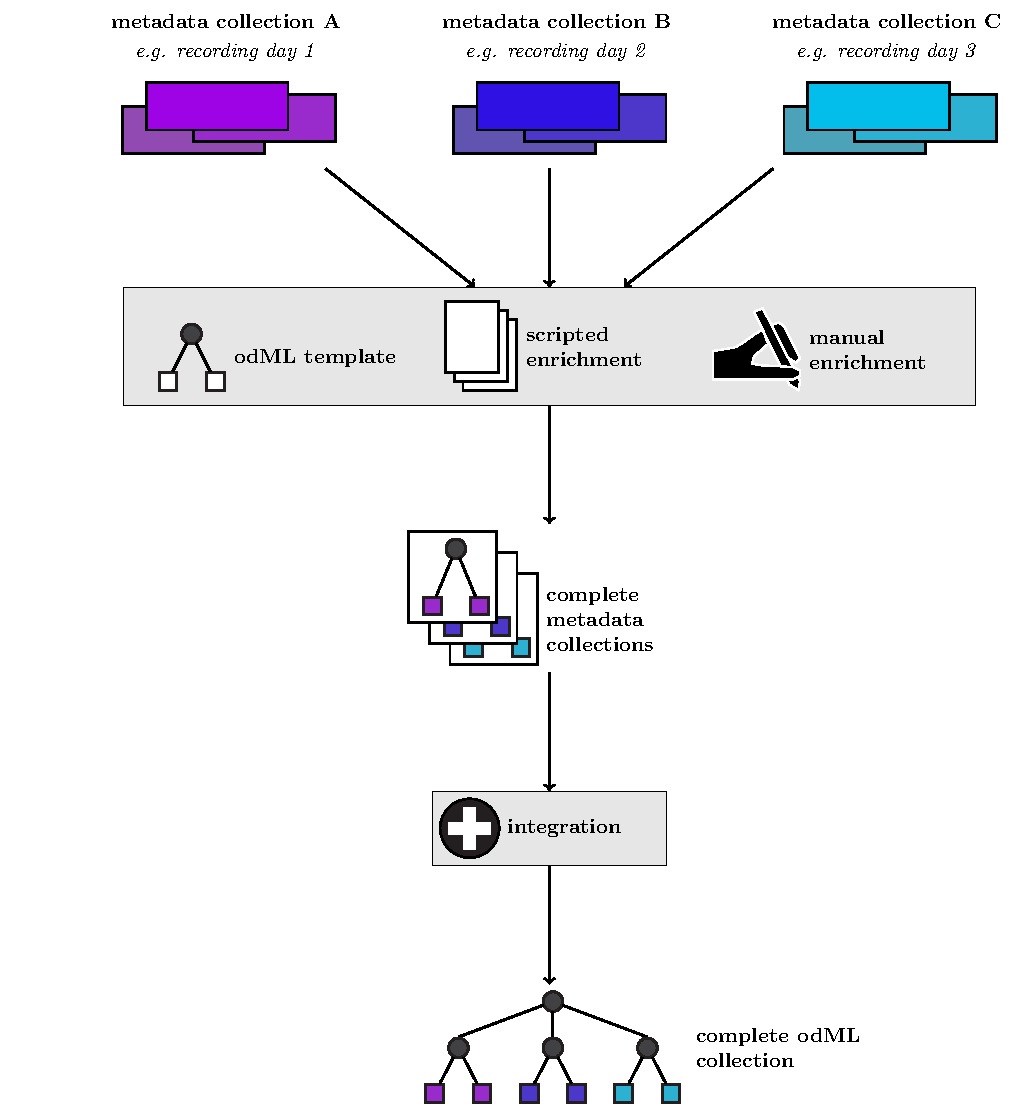
\includegraphics[width=0.70\columnwidth]{figures/odmltables_figures/fig1_odML_workflow/workflow.pdf}
\caption[Generic workflow of generating metadata collections from source files using the \software{odML} framework]{{\label{fig:odMLgeneration}
\textbf{Generic workflow of generating metadata collections from source files using the \software{odML} framework.} For a given metadata collection (top row, example metadata collections A-C), metadata are pooled from multiple files and enriched via manual entry (second row). These metadata are converted into individual collections via a scripted approach applying an \software{odML} template structure (third row). By further integrating individual multiple metadata collections (fourth row), a complete \software{odML} collection containing all recordings of a particular experiment can be created (bottom row).
}}
\end{center}
\end{figure}

\section{Software description}
\label{sec:Software}

\software{odMLtables} is a Python package that provides a set of functions for working with metadata descriptions in the \software{odML} metadata framework, with a particular focus on making these metadata easily accessible for users. The key approach is to bring the typically complex, hierarchical structure of the \software{odML} format into a tabular and reduced  representation, such that metadata can be more easily inspected or edited. Therefore, at its core, \software{odMLtables} provides functions to convert between the \software{odML} format and the corresponding tabular representation which can be represented in the \textit{Microsoft Excel} (\code{xls}) or the generic comma separated value (\code{csv}) format (\cref{fig:min_workflow}). Metadata converted to these tabular formats are accessible via widely used spreadsheet software (e.g., \textit{Microsoft Excel}\footnote{\url{https://products.office.com/en-us/excel}} or \textit{LibreOffice Calc}\footnote{\url{https://www.libreoffice.org/discover/calc/}}), such that users are able to intuitively view and edit the metadata. After editing, the metadata can be brought back to the standardized, hierarchical form defined by the \software{odML} framework (as illustrated in \cref{fig:min_workflow}).

Next to the functionality of converting between \software{odML} and the tabular formats, \software{odMLtables} provides four additional capabilities that address common tasks when working with metadata collections:
\begin{itemize}
    \item filtering (or reduction) of a metadata collection to a subset
    \item merging of two metadata collections
    \item generation of a basic \software{odML} structure to facilitate the design of a new metadata collection
    \item creating a tabular overview across multiple metadata entries within a metadata collection
\end{itemize}

The functionality of the \software{odMLtables} can be accessed in one of two ways. First, the API of the \software{odMLtables} complements the original Python \software{odML} API \citep{Grewe_2011}. As such, \software{odMLtables} simplifies the scripting of automated metadata extraction and aggregation tasks in an experiment. Second, \software{odMLtables} includes a GUI that enables non-programmers access to the large majority of functionality offered by the library. In this way, \software{odMLtables} can aid work with odML-based metadata collections in metadata workflows that do not include scripted processing stages.

In the following, we describe in detail the structure of the hierarchical and tabular metadata representations, the main capabilities of \software{odMLtables} illustrated by means of the GUI, and its internal architecture. 


\begin{figure}[!ht]
\begin{center}
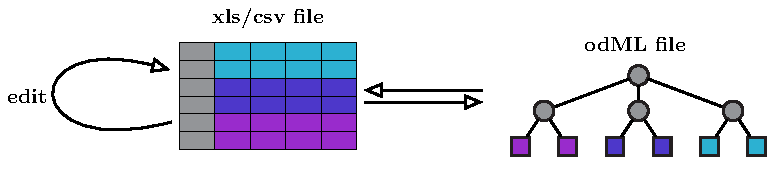
\includegraphics[width=0.70\columnwidth]{figures/odmltables_figures/fig2_odml_table_conversion/odml-table-conversion.pdf}
\caption[Minimal workflow for manually editing \software{odML} files via odMLtables]{{\label{fig:min_workflow}
\textbf{Minimal workflow for manually editing \software{odML} files via odMLtables.} Metadata is manually edited in tabular form using spreadsheet software and stored in \code{xls}{} and \code{csv}{} formats (left). The minimal functionality of \software{odMLtables} is to convert between such tabular representations and the hierarchical \software{odML} structure (right). The hierarchical placement of individual metadata entries, i.e., the Sections of the \software{odML} tree, is encoded in a specific column of the table (gray boxes and circles), whereas the values and attributes of metadata entries, i.e., a Property represented as leaves of the \software{odML} tree, are stored in rows of the table (colored boxes).%
}}
\end{center}
\end{figure}

\subsection{Hierarchical and tabular representations of metadata}
\label{sec:Hierarchical-Tabular}

\paragraph{Hierarchical metadata in the \software{odML} format}
\label{sec:subodML}

odML\footnote{\url{https://github.com/G-Node/python-odml}, RRID:SCR\_001376} is a versatile hierarchical format for metadata \citep{Grewe_2011} developed by the German Neuroinformatics Node (G-Node). While it was originally designed for electrophysiological metadata, its generic structure makes it also applicable to other scientific contexts.
% 
The basic concept is to use a tree-like structure of \textbf{Sections} to store metadata as \textbf{Properties} (extended key-value pairs) in a common \textbf{Document} (\cref{fig:odml_versions}B). For example, using this paradigm,  parameter settings of a specific device used in the experiment would be represented as Properties collected in a specific Section for that device. For a detailed tutorial\footnote{\url{https://github.com/G-Node/python-odml/blob/master/doc/tutorial.rst}} on \software{odML} please refer to the online reference documentation\footnote{\url{http://g-node.github.io/python-odml}}. The usage of \software{odML} in different environments with varying requirements has led to diversification, the identification of unused features, and the need for improvement of the original data model. In case of the \software{odMLtables} project, for example, the original internal data representation required only a subset of the complete \software{odML} data model. These and other re-implementations (NIX and RELACS projects) did not fully comply with the original specifications and led to a diversification of the de-facto implemented data models. In order to resolve this situation, with the latest release of \software{odML} version 1.4\footnote{\url{https://github.com/G-Node/python-odml/releases/tag/v1.4.0}} (i) data model and implemented features were streamlined and adapted to ensure compatibility between the various project implementations and (ii) additional features were introduced. The following paragraph briefly reviews the changes of the data model since its publication in \cite{Grewe_2011}.

\paragraph{\software{odML} model revision and streamlining}
\label{sec:odml_model_revision}
A number of features were merged or moved by the change from \software{odML} version 1.3 to version 1.4 in order to simplify usage of the \software{odML} framework as originally described in \citet{Grewe_2011}, and to mitigate potential ambiguities in the data structure. In the following, we briefly explain two major changes that affected the design and use of odMLtables. The first change was the merging of Value and Property entities (compare \cref{fig:odml_versions} A and B). This prevents value ambiguities within a Property and reduces the effective file size since the value dependent attributes ("unit", "uncertainty", "data type" and "reference") are defined only once for a set of values. This change simplified also the tabular representations of lists of values created by odMLtables. Second, for compatibility with the NIX projects' \software{odML} implementation, entities now contain a universally unique identifier (UUID, auto-generated identifier with extremely low collision probability) for unique identification of \software{odML} entities even across unrelated files to ensure comprehensive provenance tracking, including the ability to create tabular metadata representations across projects using future \software{odMLtables} versions. Compatibility for \software{odML} files using the old format version is ensured via automatized conversion functionality.
\todo{Add paragraph about empty list of values now being possible, for reference in scidata\_odmlgeneration workflow}

\begin{figure}
    \centering
    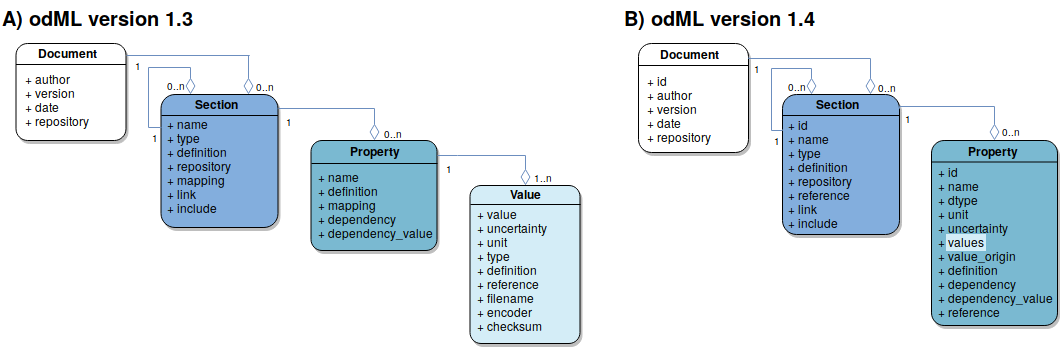
\includegraphics[width=1.0\columnwidth]{figures/odmltables_figures/fig3_odml_data_model/odML_DataModel_version.png}
    \caption[Evolution of the \software{odML} data-model]{\textbf{Evolution of the \software{odML} data-model.} Each box represents an entity defined by the data model and is color coded. Connections between entities are illustrated using the UML aggregation relation where a diamond denotes the target of a connection; the numbers at source and target denote the cardinality of each entity in the connection. (A) Version 1.3 data model. Four entities are defined: The \textit{Document} (marked in white) as the root element of a metadata file contains information about the author, document date, the document version and a default repository containing definitions used within the Document. It further contains grouping elements, \textit{Section}s (marked in dark blue). These are defined via their name and type attributes and can hold Subsections and provide semantic structure to an \software{odML} Document. The "definition" attribute provides information about the nature of a Section, while "link" and "include" refer to further Sections within the same or a different Document, respectively. Sections may contain named \textit{Property} entities (marked in cyan) which hold at least one \textit{Value} (marked in light blue) thus creating an extended key-value pair. (B) Version 1.4 data model: To simplify the use of the \software{odML} data model the Value entity was integrated into the Property taking over the attributes "dtype" (data type), "unit", "uncertainty", "value origin", and "reference". In this version a Property may contain a list of values, which must be identical in terms of the relocated attributes thus reducing the risk of ambiguities in the value list. For more information on attributes that have not been modified please refer to the original publication \citep{Grewe_2011}. Figure with permission adapted from \cite{Grewe_2011}.}
    \label{fig:odml_versions}
\end{figure}

\paragraph{Additional features}
The \software{odML} core library already provides an in-built mechanism to search and retrieve Sections, Properties or values within a Document. The need to consistently search for metadata entities across Documents from different sources led to the development of an export feature of \software{odML} metadata to the Resource Description Framework (RDF) format\footnote{\url{http://www.w3.org/TR/rdf-primer}}, a general and widely used storage format of graph databases. Multiple \software{odML} files exported to RDF can be loaded into any graph database supporting RDF and will be combined into a single graph. Moreover, while XML is still the default storage format, \software{odML} now additionally supports storing the metadata in the text based file formats JSON\footnote{\url{https://json.org}} and YAML\footnote{\url{https://yaml.org}}. JSON has become a de-facto data exchange standard between web based and standalone computer applications. The support of JSON makes \software{odML} metadata more easily consumable in machine-only workflows through modern applications. Since both XML and JSON primarily aim at machine-readability, their structure is not easily readable by humans. To ease reading of raw \software{odML} files by actual persons the YAML file format support was added.

For easy visualization and manipulation of specific \software{odML} files, the graphical user interface of \software{odMLtables} was integrated into the native \software{odML} GUI (odml-ui\footnote{\url{https://github.com/G-Node/odml-ui}}). Thus, the \software{odML} GUI now grants direct access to the main \software{odMLtables} features, making both software tools even easier to use back to back for both browsing and editing of metadata.

\paragraph{Tabular representation of the \software{odML} format} 
\label{sec:tabular_format}

\software{odMLtables} converts the hierarchical \software{odML} structure (\cref{fig:tree_and_table}A) into a specific tabular (flat) representation (\cref{fig:tree_and_table}B), stored either in the \code{xls} or \code{csv} format. In this format, each row corresponds to one particular value entry. The columns further describe the Property and Section each value belongs to, e.g. the Property name, the Section and Subsections the Property belongs to, the physical units, or the Property definition. The hierarchy of Sections in which a Property is located in the original \software{odML} structure is represented by a path construct, where individual Section names are delineated by the '/' character. For increased readability, repetitive information (i.e. identical information to the cell above) is optionally displayed only at the first instance (e.g., 'Path to Subject' entry ('/Subject') in row 3, 4 and 5 in \cref{fig:tree_and_table}B). By default, the  column headers are predefined (\cref{fig:tree_and_table}B, first row), however the header names can also be customized as long as a mapping between the predefined names and the custom names can be provided. The order of the columns of the table can be customized since the column header names are used to associate columns with attributes of the hierarchical \software{odML} structure. The \software{odML} Document attributes 'author', 'date', 'version' and 'repository' are handled separately and are placed in the top row of the tabular \software{odML} representation.

\begin{figure}[!ht]
\begin{center}
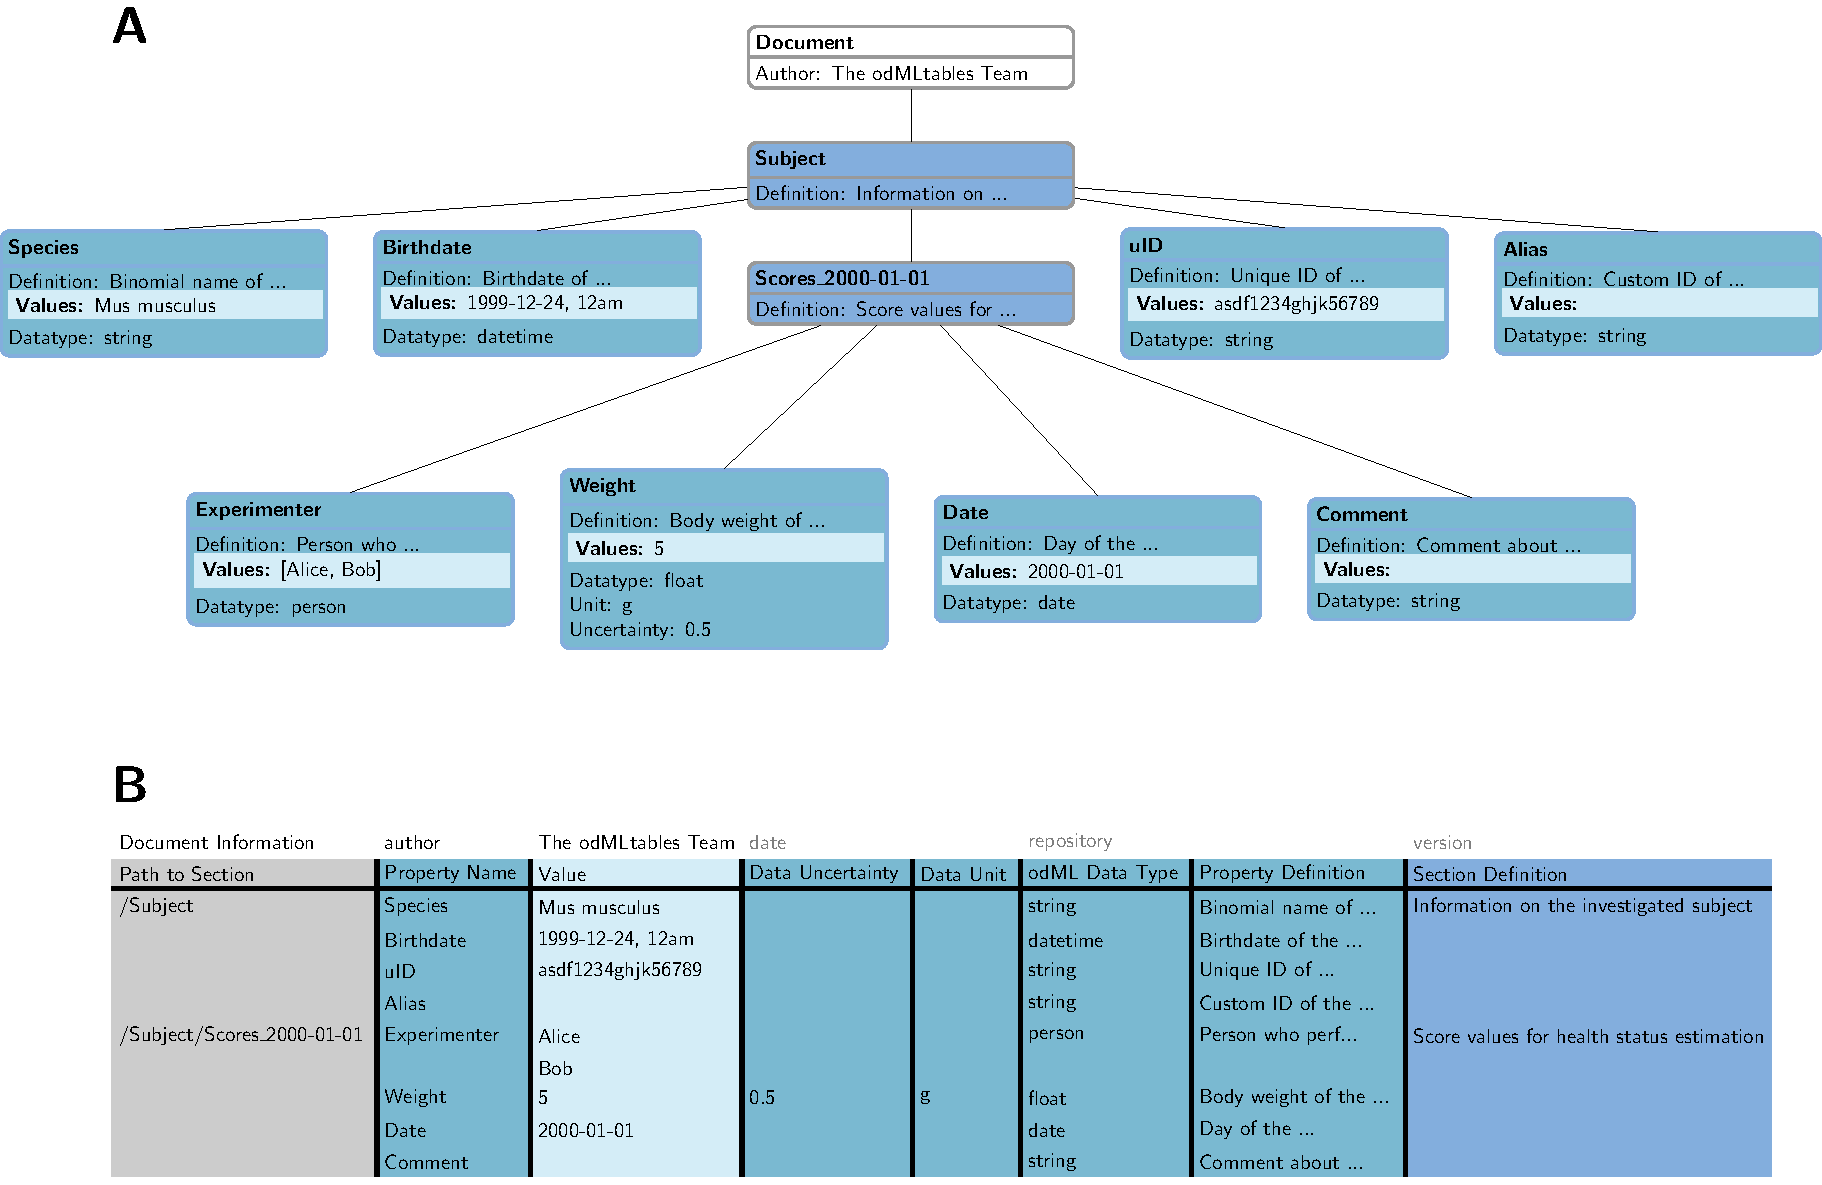
\includegraphics[width=1.0\columnwidth]{figures/odmltables_figures/fig4_hierarchy_table_mapping/hierarchy_table_mapping.pdf}
\caption[Mapping of an \software{odML} structure in (A) hierarchical metadata format to (B) tabular format.]{{\label{fig:tree_and_table}
\textbf{Mapping of an \software{odML} structure in (A) hierarchical metadata format to (B) tabular format.} Individual attributes of the \software{odML} entities are represented in different columns in the tabular representation (e.g. 'Section Definition', 'Property Name', 'Data Uncertainty', compare color code). Document attributes ('author', 'date', 'repository' and 'version') are described separately in the first row of the tabular representation. The hierarchy of Sections is captured in an additional column ('Path to Section') describing the path between the \software{odML} Document and the current Section. Each metadata entry in the hierarchical format corresponds to a single row in the tabular format. Items of a list are treated as individual entries.
}}
\end{center}
\end{figure}

\subsection{Software Functionalities}
\label{sec:software_functionalities} 

\software{odMLtables} is a tool that provides 5 functionalities surrounding work in creating and accessing metadata collections. In the following, we describe the capabilities of these features, while their use is put into the context of a typical workflow in \cref{sec:Illustrative-Examples}.

All main features of \software{odMLtables} are available via the \software{odMLtables} GUI (\cref{fig:GUI_mainwindow}). Upon launching the application, it presents the user with 5 buttons, each leading to a series of dialogs (wizards) to perform a specific \software{odMLtables} functionality. For the more complex dialogs that include a large number of parameters to set, the GUI offers to save and load the dialog configuration to efficiently re-run a functionality with given parameters. 

In addition to the functionality offered by the GUI, the Python programming interface of \software{odMLtables} offers additional features, most notably, the ability to customize the default values for \software{odML} data types. The default values can be displayed using a highlighted coloring scheme to indicate to the researcher that a Property currently contains a default value (for details, see the \software{odMLtables} documentation\footnote{\url{https://odmltables.readthedocs.io}}).

\def\fconvert{F1}
\def\fgenerate{F2} 
\def\fcompare{F3}
\def\fmerge{F4}
\def\ffilter{F5} 

The main features of \software{odMLtables} are described in detail below and are referred to as feature \fconvert - \ffilter:


\textbf{\fconvert: Convert between \software{odML} and table format.}
This function converts metadata collections between the representations in the different file formats odml, \code{xls}, and \code{csv}. For the conversion to and from the tabular formats (\code{xls}/\code{csv}) a specific formatting of the table is required in order to interpret the table as hierarchical \software{odML} structure (see \cref{sec:tabular_format}). Nevertheless, \software{odMLtables} allows for a certain degree of flexibility in order to give researchers the ability to design tabular formats to best fit their workflow. In particular, this encompasses the inclusion or removal of certain optional columns, the arrangement of columns, column headers, or the coloring scheme. Note however, that for the reverse conversion from a tabular format back to the \software{odML} format, these customizations need to be known (e.g. custom column names, see \cref{sec:Template-Generation}).

\textbf{\fgenerate: Generate new metadata collection table.} This function generates and saves an empty, generic (template) \software{odML} structure in the \code{xls} format. This generic structure provides a good starting point to design a metadata collection or template structure in a tabular format providing the required tabular structure for conversion to a hierarchical \software{odML} structure. Similar formatting options can be applied to the table as indicated above.

\textbf{\fcompare: Generate overview across entries within a metadata collection} This function creates a chart listing multiple entries within a single metadata collection. It is intended to develop overview sheets containing similar Properties, e.g. the animal weight at different ages. The generated table does not follow the tabular \software{odML} format and can therefore only be used for visualization and not for conversion into the hierarchical \software{odML} format. Using common spreadsheet software the comparison table can be saved as a figure and printed for usage in a laboratory notebook.

\textbf{\fmerge: Merge contents of two metadata collections} This function allows to merge multiple files (\software{odML} format) into a single file. Here, by default, Sections, Properties and values are added to existing entities during merging. However, for values of coinciding Properties the option exists to overwrite values during the process of merging.

\textbf{\ffilter: Filter content of a metadata collection} This function reduces the size of an \software{odML} file based on a filter mechanism, which can include multiple steps of filtering and custom filter functions to select only specific parts of an \software{odML} structure. The filter mechanism e.g. can extract all Properties containing no values to present the experimenter potential missing entries in the metadata collection.


\begin{figure}[!ht]
\begin{center}
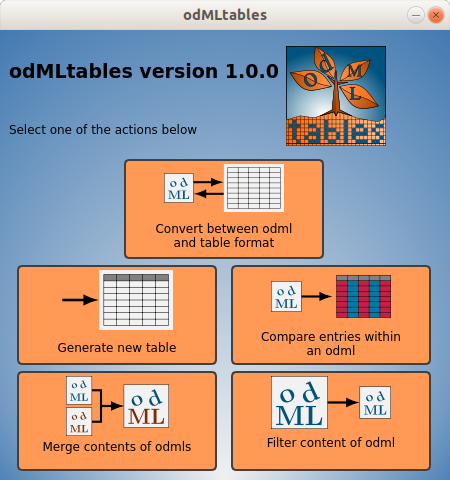
\includegraphics[width=0.70\columnwidth]{figures/odmltables_figures/fig5_odMLtables_screenshot/Screenshot.png}
\caption[Main window of the \software{odMLtables} GUI]{{\label{fig:GUI_mainwindow}
\textbf{Main window of the \software{odMLtables} GUI}. The interface gives access to the main functionalities available by the tool: Converting files from hierarchical to tabular (flat) representations, generating an empty generic \software{odML} table (template), comparing entries within a metadata collection, merging contents of two collections, and selecting a subset of a metadata collection (filtering). Each button starts a series of dialogs (wizards) that guide the user through the corresponding process.
}}
\end{center}
\end{figure}

\subsection{Software Architecture}
\label{sub:Software-Architecture}

In the following, we explain the internal structure of the \software{odMLtables} software. For a detailed description, see the function reference in the \software{odMLtables} documentation.

The core of \software{odMLtables} is the \texttt{OdmlTable} class, which provides the main functionality for loading and saving metadata collections in the different file formats. It implements basic operations on the loaded metadata independent of the file format they originate from. Within the class, metadata are internally represented as a list of dictionaries, where each dictionary corresponds to an \software{odML} Property. Functions that modify the metadata collection, like merging and filtering, act directly on this internal dictionary representation. The two tabular formats \code{xls} and \code{csv} require additional information regarding the table layout when being saved to disk, e.g., the color scheme. Therefore, two subclasses of the \texttt{OdmlTable} class (\texttt{OdmlXlsTable} and \texttt{OdmlCsvTable}) carry these additional output settings. Finally, a separate \texttt{CompareSectionTable} class implements the function for comparing Properties within one \software{odML} structure. As for the \texttt{OdmlTable} class, two specific subclasses for \code{xls} and \code{csv} output are defined to capture layout information (\texttt{CompareSectionXlsTable} and \texttt{CompareSectionCsvTable}).

One feature of \software{odMLtables} in generating \code{xls} files is to highlight a value entry if it corresponds to the default value of the corresponding Property's data type. However, the \software{odML} library itself does not specify such default values for all of its data types. Moreover, it is not mandatory, nor always desired, to specify a data type in the \software{odML} in all circumstances, e.g., when leaving a value empty. Therefore, \software{odMLtables} provides functionality to work with default values for data types in the \texttt{OdmlDtypes} class. It manages the data types, synonyms, default values, and value conversions. The class is used for entering default entries when loading empty values from a tabular representation, and for default value highlighting.

In addition to the core module, \software{odMLtables} provides a GUI that exposes most functionality of the core module. The GUI is based on the PyQt5\footnote{\url{https://wiki.python.org/moin/PyQt}} framework and consists of a main window (\cref{fig:GUI_mainwindow}) and five wizards (see \cref{sec:software_functionalities}). Each wizard inherits from the \texttt{OdmltablesWizard} class, which provides helper functions and error handling. The \texttt{Settings} class stores the current user settings for calls of \software{odMLtables} core functions, and provides functionality to save and restore user settings between different executions of the GUI.


\section{Embedding \software{odMLtables} in data acquisition and analysis}
\label{sec:Illustrative-Examples}

While most scientists would agree that accurate records of the minute details of an experiment are the foundation of good scientific practice, in the everyday routine of an experimental electrophysiology lab it is difficult for the scientist to record, sort, and maintain the wealth of metadata information that accumulates during an experiment. While the \software{odML} format is suitable for storing metadata information from different sources, lacking to date is a set of tools that allows the scientist to create, manipulate and visualize the data stored in this format. In the following, we present commonly encountered scenarios involving metadata handling that originate from our collaborative work. These scenarios touch the issues of how to design the hierarchical structure to store and organize the metadata, how to practically enter metadata before, during or after the experiment, and how to create a comparison of rich metadata buried within the \software{odML} structure. It turns out that for each of these scenarios a flattened tabular representation of the metadata is a practical solution that feels intuitive to the user. In the following we demonstrate how to implement these scenarios that consist of combining operations in \software{odMLtables} and a spreadsheet program. All scenarios are also available as an interactive Jupyter Notebook\footnote{\url{https://jupyter.org/}} accessible via the \software{odMLtables} documentation\footnote{\url{https://odmltables.readthedocs.io/en/latest/tutorial.html}}.

\subsubsection*{Scenario 1: How to generate a metadata template without programming}
\label{sec:Template-Generation}
In conducting animal experiments, a typical scenario where metadata are collected manually on a daily basis is the creation of an animal \textit{score sheet}. Such score sheets record quantitative, and in part also qualitative, measures that are collected in order to document and judge the animal's health and state over the duration of the experiment. Often, these sheets are an obligatory piece of documentation of the experiment, such that only the availability of a defined workflow to create score sheets guarantees their consistency over multiple years and different experimenters. For example, for mouse experiments, typical measures are the body weight, water intake and breathing frequency, many of which can be used to assess the health of an animal, e.g., by calculating a health score for each mouse \citep{Foltz_1999, Burkholder_2012}. In \cref{fig:tree_and_table} we depicted how metadata of a single, minimized score sheet can be integrated into an \software{odML} document containing collective information on a subject.

The measurements for such score sheets are typically easy to perform, and for this reason may be conducted by a number of different people in the lab. Therefore, the daily process must be simple, intuitive, and robust in order to be conducted by all members of the group. Collecting the information in a table format using common spreadsheet software tools, such as \textit{Microsoft Excel} or \textit{LibreOffice Calc}, satisfies these requirements. 

To guarantee a consistent structure of such a score sheet, initially a template needs to be set up, i.e., a table containing the measures that are to be recorded on a single day. In order to accomplish this, as a first step we generate an empty template table using odMLtables. To improve the readability, we enter custom column names in \software{odMLtables} to create the table ('Section' instead of 'Path to Section', 'Measure' instead of 'Property Name', 'Unit' instead of 'Data Unit', and 'Type' instead of '\software{odML} Data Type'). Also we omit the attributes 'Section Definition', 'Property Definition' and 'Data Uncertainty' in the context of these example scenarios. As second step, using a spreadsheet, we design the metadata structure for a single score sheet as shown in \cref{fig:template_table}. The value field for each entry can be either left empty or a default value can be entered. The latter case is interesting for values that are likely to be constant for the majority of experiments, e.g., the name of the experimenter. Since the colors of a table saved in the \code{xls}{} format are ignored when converting to the \software{odML} format, it is possible to use arbitrary color coding within the spreadsheet software to improve the readability of the table for the experimenters entering the values.

\begin{figure}[!ht]
\begin{center}
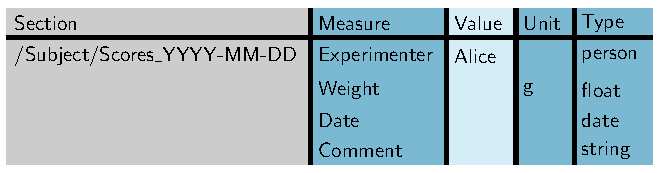
\includegraphics[width=0.5\columnwidth]{figures/odmltables_figures/fig6_template_table/template_table.pdf}
\caption[Template score sheet]{\label{fig:template_table}
\textbf{Template score sheet.} The template score sheet contains the measures required for each measurement day, including optional default values (here: ``Alice'' for ``Experimenter'' and ``g'' as unit for ``Weight'').}
\end{center}
\end{figure}

We designed the template table such that it matches the properties of the minimized score sheet section already depicted in \cref{fig:tree_and_table}. Notice that in the template the entry for column 'Section' already includes a parent section to reference the animal (cf.,~\cref{fig:tree_and_table}). This is convenient for defining the position of each score sheet in the \software{odML} hierarchy to simplify a later merging process (cf., scenario 2).

\subsubsection*{Scenario 2: Collecting daily observations in a common \software{odML} structure}

Once the template from scenario 1 is complete, it is copied to a new file on each measurement day, and the copy is filled out by the person taking the measurements. To avoid that metadata are spread across multiple files and potentially multiple locations, we aim to gather the data from multiple days into a single \software{odML} file. To achieve this, we use \software{odMLtables} to first convert the individual \code{xls} file containing an individual score sheet into the \software{odML} format, and to subsequently merge these into a common \software{odML} structure spanning multiple recording days.

Specifically, the conversion from the \code{xls} to the \software{odML} format we use the \software{odMLtables} feature \fconvert\ (for details of \software{odML} features \fconvert - \ffilter, see \cref{sec:software_functionalities}). After the conversion, the current score sheet present in \software{odML} format is merged into the common \software{odML} document collecting the complete information of an animal using feature \fmerge \ on a daily basis. This extends the \software{odML} structure of the subject document by an additional Section each recording day. Note that this is possible because the first column of individual score sheets (\cref{fig:template_table}) not only provides a unique Section name for each score sheet, but also indicates the location of the \software{odML} Section in the hierarchical structure of the subject document, (e.g., ``Subject/Scores\_2000-01-01''). The result is a single \software{odML} file containing measures collected on all recording days while the source files generated each day can be archived.

The metadata collection containing the merged score sheets of 2 recording days might look like the following:

\begin{minipage}[t]{\textwidth}
\dirtree{%
.1 Document "mouse-score-sheets". 
.2 Section "Subject".
.3 Property "Species": Mus musculus.
.3 Property "Birthday": 1999-12-24 12:00:00.
.3 Property "uID": asdf1234ghjk56789.
.3 Property "Alias":.
.3 Section "Scores\_2000-01-01".
.4 Property "Experimenter": ["Alice", "Bob"].
.4 Property "Weight": 5g.
.4 Property "Date": 2000-01-01.
.4 Property "Comment":.
.3 Section "Scores\_2000-01-02".
.4 Property "Experimenter": "Bob".
.4 Property "Weight": 5.5g.
.4 Property "Date": 2000-01-02.
.4 Property "Comment": "Small scratch at the right ear".
}
\ \\
\end{minipage}

\subsubsection*{Scenario 3: Create a tabular representation of the \software{odML} file for better viewing using the color options}
Once the recordings for a number of animals were performed and the corresponding metadata collection is completed, data and metadata should be shared among collaborators in a common repository. In order to get an overview of the data obtained across different animals, the metadata of each animal can be converted into the \code{xls} format to simplify the inspection of the associated metadata using spreadsheet software (cf., also, \cref{fig:tree_and_table}B). Here, \software{odMLtables} provides the option to use color coding and highlighting of default / missing values to improve the readability (\cref{fig:missing_values_table}).

\subsubsection*{Scenario 4: How to filter a subset of an \software{odML} file to edit it later on}
As the common \software{odML} structure grows day by day it is of advantage to extract specific subsets of \software{odML} values of interest for visualization using the tabular format. Instead of visualizing the whole metadata collection to periodically verify that all Properties are filled with a value, we can extract a subset of the collection and visualize only the relevant (e.g. empty fields) entries. For this, we use \software{odMLtables} feature \ffilter\ which can be used to generate an \software{odML} that contains only Properties without value information specified. We then convert this reduced \software{odML} into a tabular \code{xls} representation using \software{odMLtables} feature \fconvert. The generated table, as shown in \cref{fig:missing_values_table} indicating the two empty properties in the \software{odML} structure of scenario 2, can be visualized using spreadsheet software and, in case of values not being filled, these can be directly edited manually.

\begin{figure}[!ht]
\begin{center}
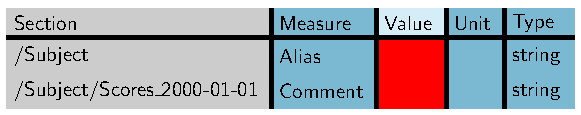
\includegraphics[width=0.5\columnwidth]{figures/odmltables_figures/fig7_missing_values_table/missing_values_table.pdf}
\caption[Metadata collection filtered to show only Properties with an empty value]{\label{fig:missing_values_table}
\textbf{Metadata collection filtered to show only Properties with an empty value.} Missing values entries are highlighted in red by odMLtables.}
\end{center}
\end{figure}

\subsubsection*{Scenario 5: Merging the edited subset back into the original structure}
The enriched \code{xls} sheet generated in step 4 should now be merged back into the common \software{odML} structure. For this, we convert it back into the \software{odML} format and use the \software{odMLtables} merge feature \fmerge\ to replace the edited values in the common \software{odML} structure with the edited ones. Here, \software{odMLtables} merges the two \software{odML} files by extending the \software{odML} structure and appending metadata entries when the same Property is present in both files. However, when modifying already existing metadata entries in the filtered version this would result in duplication of entries. Therefore, \software{odMLtables} offers the possibility to overwrite already existing metadata entries when merging two \software{odML} structures. Note that a selective merge of a subset of metadata can be achieved by first filtering the file to be merged using feature \ffilter\ . 


\subsubsection*{Scenario 6: Compare entries in the \software{odML} file for data screening and lab book usage}
In addition to the complete metadata representation as presented in scenario 3, it is possible to generate a reduced overview table containing only plain values of selected Properties. This feature can be used to create a tabular display of Properties of interest (e.g., weight of a specific animal, experimenter who performed the experiment and comments regarding the measurement) in rows for the individual recordings (days) in columns. An example of such a table is given below:

\begin{center}
\begin{tabular}{|l||l|l|l|}
\hline
				 & Scores\_2000-01-01 & Scores\_2000-01-02\\
\hline
Date             &  2000-01-01 & 2000-01-02\\
\hline
Weight           &  5.0g & 5.5g\\
\hline
Experimenter     & Alice, ... & Bob\\
\hline
Comment  & Blood sample was taken [...] & Small scratch at the right ear \\
\hline
\end{tabular}
\end{center}

This type of overview tables can also be printed and used as part of the mandatory documentation of the experiment in a written or printed lab book. This way, the recorded data only need to be documented once in a digital fashion and consistency between documentation and digitally available metadata is guaranteed. 

\subsubsection*{Scenario 7: Automatized processing of metadata collections}
After completion of an experiment covering many recording days, the processing steps presented in scenarios 1-6 can be performed in an automatized fashion on the complete metadata collection to generate a comprehensive metadata document and corresponding overviews. While it is possible to perform this action using the graphical user interface, an automated approach has the advantage that it can be repeatedly executed when one of the original files changes, e.g., by a retrospective update of metadata or loss of the generated metadata files. In addition an automated approach is more robust against errors introduced by the manual operation and can be at least partially reused for subsequent experiments.

By use of the \software{odML} library together with the \software{odMLtables} Python API, users have a rich collection of functions to manipulate and convert metadata stored in the \software{odML} format. In this specific example, we show an example script in \cref{code:odmltables} that loads all daily animal score sheets, adds them to a common metadata structure and exports the final document into an overview and comparative \code{xls} sheet for visualization. The code demonstrates the metadata handling workflow by structuring it into a sequence of three generic functions, which can be of use in creating related workflows for different projects.


\begin{codeenv}
\inputminted[linenos,tabsize=2,breaklines, fontsize=\scriptsize]{python}{figures/code_odmltables_automation.py}
\caption[Assemble metadata using \software{odMLtables}]{Program to assemble a target \software{odML} document covering metadata of multiple recording days by pooling information from multiple \code{csv} files and generate visualizations and overviews. Individual functions are automatizing functionalities presented in previous scenarios.}
\label[codelisting]{code:odmltables}
\end{codeenv}



\subsubsection*{Improved handling and visualization of complex metadata structures}
Up to now we demonstrated the basic mechanisms of \software{odMLtables} based on highly simplified examples presented above. In a real world example, however, metadata collections are inherently complex and corresponding metadata collections can easily encompass thousands of values. A publicly available example of this are electrophysiological recordings of macaque monkeys performing a reach to grasp task that include a rich metadata collection stored in the original \software{odML} files as well as the corresponding \code{xls} representation created by \software{odMLtables} \citep{Brochier_2018}. We demonstrate the usage of \software{odMLtables} to select and visualize a subset of the complete metadata collection as well as generation of overview tables in an interactive Jupyter Notebook in the \software{odMLtables} documentation\footnote{\url{https://odmltables.readthedocs.io/en/latest/tutorial.html}}.

\section{Discussion}
\label{sec:Discussion}

We presented the \software{odMLtables} software, which facilitates the use of the \software{odML} metadata format in everyday experimental and data analysis work. In scenarios 1 to 7 we present the features of \software{odMLtables} within a simplified real world example, namely the definition of an animal score sheet and with this the controlled routine collection of corresponding metadata. More specifically, we showed in scenario 1 the setup of a template for an animal score sheet in the \code{csv} format and its conversion to \software{odML} (\fconvert, \fgenerate). In the next scenario, we used this template to routinely collect the animal's health measures and aggregated them in a single \software{odML} file per animal (\fconvert, \fmerge). Besides a simplification of metadata acquisition in the \code{csv} format,  we showed in scenario 3 the benefits of a colored tabular representation for visual inspection of the collected score sheets (\fconvert). In scenario 4, we demonstrated how supplements of metadata values can be easily added by extracting a the missing metadata entries from the complete collection (\ffilter). Subsequently we demonstrated in scenario 5 the integration of the amended metadata back into the complete collection (\fmerge). We generated a compressed overview table, summarizing the metadata from different routine collections in a concise, laboratory notebook suitable fashion in scenario 6 (\fcompare). Finally, in scenario 7 we discussed the amortization of the workflow presented in the previous scenarios and provided code examples showcasing the \software{odMLtables} Python interface.

As \software{odMLtables} can be used by programmers and non-programmers alike, \software{odMLtables} simplifies the development of comprehensive metadata management in the scientific community by offering user-friendly interaction with the \software{odML} format. In this way, its usage is intended to improve reproducibility and replicability of experiments and to facilitate cooperative work, both within labs and across different laboratories. Complementing the model scenarios above, in \cref{fig:global_workflow} we summarize and generalize the use of individual components of \software{odMLtables} during the course of an entire experiment. Although the presented scenarios are set in a neuroscientific environment, \software{odML} and \software{odMLtables} are indifferent with respect to the scientific discipline and can therefore be used for metadata management in different contexts. In the following, however, we discuss specifically its embedding into a tools landscape developing in the field of electrophysiology.

Although, the real world workflow described in \cite{Brochier_2018} and \cite{Zehl_2016} as well as the minimalistic workflow presented here are all set in the field of animal experiments covering multiple days, \software{odML} as well as \software{odMLtables} can be used for metadata management in a broader context. For example in the context of experimental research the benefits of \software{odMLtables} can be seen at all stages of an experiment: from setting up a specific metadata structure in the preparatory phase, manual enrichment of the metadata collection during the experiment, through to the generation of overviews and summaries from metadata collections during data analysis. Also, for publicly available datasets with an \software{odML} metadata collection, \software{odMLtables} can be used to create a tabular representation of the \software{odML} files to quickly scan the metadata of the experiment.

\subsection{Performance estimation}
Since the release of the original version, \software{odML} has been used in various projects for storing metadata as they become available during data acquisition or analysis (e.g. in the NIX\footnote{\url{https://github.com/G-Node/nix}, RRID:SCR\_016196} and RELACS\footnote{\url{https://github.com/relacs/relacs}} projects), as metadata schema in the EEGbase database\footnote{\url{http://eeg2.kiv.zcu.cz:8080/home-page?1}, RRID:nif-0000-08190} (see also \citealp{Moucek_2014}), and as a part of the metadata data pipeline as described by \cite{Zehl_2016} and \cite{Brochier_2018}. The advantage gained by comprehensive metadata management using \software{odML} can be demonstrated by a small example based on a published dataset \citep{Brochier_2018} for which detailed metadata are stored in the \software{odML} format. Accessing information about the number of neurons recorded on different electrodes contained in the \software{odML} files using common desktop hardware requires approximately 0.5 seconds for this dataset using the \software{odML} iteration and filter mechanism. Extracting the same information not from the \software{odML} metadata but from the original data files using the Python library \software{Neo} version 0.7.1\footnote{\url{https://github.com/NeuralEnsemble/python-neo/releases/tag/0.7.1}} requires about 25 seconds using the \software{Neo} filter and annotation mechanism. Comparing these times, the usage of \software{odML} in this example gives a speedup of a factor 50. However, for a fair comparison also the time for \software{odML} generation needs to be taken into account, which for a dataset of this complexity is typically on the order of 10 minutes, considering that the generation process needs to read the data files and a number of associated files \citep{Zehl_2016}, perform various quality checks or automated preprocessing checks. Comparing this conservative estimate of the generation time of the \software{odML} file, the access time using the \software{odML} format and the access time using the original data files shows that using the \software{odML} format pays off after 25 times of metadata access. This is a relatively small number of metadata accesses for a single dataset considering the relevance of metadata in multiple steps of the experiment, e.g. exploratory analysis and parameter scans in analyses runs, and collaborative work, where different people access the same metadata on different computers. In the latter setting using \software{odML} is also of advantage because the potentially large original data files might not be present on all computers of all collaborators, whereas \software{odML} files are much smaller in file size and can therefore be shared more easily, e.g., via a version control system like git\footnote{\url{https://git-scm.com}}.

\subsection{\software{odMLtables} as conversion tool}
One may argue that extending the existing \software{odML} editor to support a flattened view on the metadata is a more direct and efficient way to implement tabular representations, as opposed to a converter (such as odMLtables) between formats. However, such a solution has direct implications on (i) the maintainability of the tool, (ii) its adoption by the community, and (iii) its interoperability in the heterogeneous types of workflows typically encountered in data acquisition. Regarding (i), the development of graphical editors for tabular data  is a time-consuming endeavor and leads to a complex code base that is difficult to maintain. This is even more true in a scientific environment, where software maintenance is often left to persons who are not expert in GUI programming and design patterns for graphical applications. Regarding (ii), spreadsheet software is already commonly used in laboratory environments to track metadata, and experimental scientists are used to efficiently use these tools in their daily routine. Therefore, integrating such software in a digitized workflow, rather than proposing an entirely new user-facing tool, is bound to lower the threshold for adoption in a laboratory. Finally, regarding (iii), data acquisition workflows in an experimental environment are often subject to constraints set by the individual formats in which metadata are generated by the components of the experimental setup. Tabular representations, and in particular those stored in the \code{csv} format, represent \textit{per-se} one of the most commonly encountered and most simple formats to exchange data. Indeed, the capability to read \code{csv} data files is provided by the standard libraries of many programming languages, in particular those commonly used in data analysis and scientific computing, such as Python, Matlab, or R. Therefore, being able to convert between human readable tabular metadata generated automatically by various metadata sources of the experiment and their joint representation in a hierarchical \software{odML} metadata collection is helpful in creating a metadata acquisition workflow that is interoperable with the various components of the experiment. Combining such workflows with version control systems, such as git, to store the hierarchical or tabular metadata representations is a viable option to enable collaborative creation of metadata records, in particular when considering the text-based \code{csv} or and \software{odML} formats.

\subsection{Relation to electronic laboratory notebooks}
One particular case where flexible interoperability is in demand are electronic laboratory notebooks (ELNs) which are available from a large range of manufacturers and are becoming increasingly utilized by laboratories \citep{Kwok_2018}. Their design is actively being researched in the process of digitizing the research process \citep{Kanza_2017}. ELNs are software tools originally designed to replace the hand-written lab book used in experimental sciences to document experiments, outcomes and analyses by providing a method to electronically enter such metadata in a digitally signed and potentially encrypted fashion that ensures protection from falsification. Some ELNs go beyond this functionality by integrating tightly with laboratory inventory management systems (LIMS) or analysis pipelines (comparisons of selected ELNs can be found in \citep{Rubacha_2011} and various web resources
\footnote{\url{https://datamanagement.hms.harvard.edu/electronic-lab-notebooks}}
\footnote{\url{https://www.labfolder.com/electronic-lab-notebook-eln-research-guide}} \footnote{\url{https://www.gurdon.cam.ac.uk/institute-life/computing/elnguidance}}). One major advantage of ELNs that store hard metadata \citep{Grewe_2011} in form of key-value pairs is that they can be directly digitally accessed in analysis scripts, rather than having to manually copy the information from the hand-written lab book \citep{Zehl_2016}. While for some disciplines specialized lab notebook software packages have been developed \citep{Kwok_2018} that are aware of community standards for storing such metadata, most of these packages come with their own format for storing data that can only be accessed via file export functionality or specific APIs. In some disciplines this may be of little importance, since either the metadata records stored in the ELN are not required in the analysis process, or the metadata are captured using a domain-specific ELN that is integrated with functionality to directly perform the analysis steps from within the ELN. Nonetheless, other disciplines, such as neurophysiology, require detailed metadata available in an environment suitable for performing complex, exploratory analysis protocols that go beyond the capabilities of currently available ELNs. Here, \software{odML} is a potential candidate for implementing such features. In absence of a global standard to record metadata, \code{csv} represents one of the de-facto standards to export metadata from ELNs in a universal format. For this reason, the conversion to \software{odML} via \software{odMLtables} provides access to metadata recorded with ELNs for external analysis pipelines that rely on hierarchically structured metadata collections. The same holds true for the reverse direction, where metadata generated by tools building on the \software{odML} specifications can be imported into an ELN. For example, the feature of \software{odMLtables} to create tabular overviews of the metadata (feature \fcompare, see \cref{sec:software_functionalities}) would allow to generate current overview tables in terms of animal score sheets as \code{csv} that could be directly (and assuming the ELN has an API, even automatically) integrated into the documentation of an experiment contained within an ELN, assuming only basic \code{csv} import capabilities. 

Beyond ELNs, labs increasingly resort to institution-wide databases to manage and record their research activities, and, in some cases, even the data as such. Depending on the architecture, some systems are likely to implement data imports using tabular schemata. One example of such a tool implementing database and processing functionality is DataJoint\footnote{\url{https://datajoint.io/}, RRID:SCR\_014543} as a tool to assist in ingesting, combining and analyzing heterogeneous data in a relational database \citep{Yatsenko_2015}. It is easy to populate a DataJoint database using tabular data, as described in detail in the accompanying online documentation. For example, one may extract a subset of the metadata in form of a comparison table using the \software{odMLtables} feature \fcompare, and then incorporate this table into a larger DataJoint database spanning all experiments using a generic function for populating from \code{csv} tables. In such a fashion, \software{odMLtables} presents a gateway to integrate structured metadata by the diverse tools used in a laboratory to organize the record keeping of an experiment.

\subsection{Outlook}
The current version of \software{odMLtables} provides a set of core functions that were identified as necessary in co-designing various data and metadata acquisition workflows in collaboration with multiple laboratories spanning different types of experiments and data modalities. Nevertheless, a number of additional features are envisioned as a result of feedback stemming from these collaborations to extend the range of applications for the tool and enhance its flexibility for heterogeneous metadata workflows. In addition, feature requests are welcome on the project's issue system on github. One next step will be to extend the capability to create tabular comparisons (feature \fcompare) across metadata stores in multiple files. This would give researchers the option to query for metadata that are distributed over several, even differently structured, \software{odML} files. For example, in chronic recordings of brain activity accumulated over the course of multiple months, researchers may decide to generate a single \software{odML} file per recording day, and may want to utilize such a functionality to compare the number of trials and other performance measures across the entire recording period.

A second planned feature addition to odMLtables, related to the previous aspect, is the ability to create complete tabular representations (i.e., feature \fconvert) across multiple \software{odML} files, and vice versa. To this end, one may implement an additional column next to the \software{odML} path and Property name that indicates the file in which a certain metadata entry is found. As an example application, one may consider a complex experiment where metadata originating from different parts of the experiment are stored in separate \software{odML} files, but a large overview table is desired for manually browsing the metadata. While this is already possible by merging (\fmerge) individual files and then converting (\fconvert) the table, the information about the origin of metadata in the original file structure is lost.

A third feature addition to \software{odMLtables} is the automatic generation of Python code based on the steps the user performs in the graphical user interface. For example, this may yield the Python code to perform a certain filter operation designed in the GUI. This would simplify the automation of metadata processing without specific knowledge about the \software{odMLtables} API.

For communicating the structure of a complex metadata collection to new collaborators neither tabular nor hierarchical views have been found to be efficient. For this, a graphical representation of the metadata structure is likely to be more useful, especially for large metadata collections. For this reason, a fourth addition to \software{odMLtables} would be to introduce a common graphical representation as new output conversion format.

Lastly, as a fifth feature addition, \software{odMLtables} could assist scientists in defining the links between data and metadata in an experiment. Typically, several metadata are accumulated from various sources in an experiment that are directly related to one particular part of the data, and in fact, may be crucial in performing data analysis. For example, the signal recorded from a particular electrode may contain the impedance as measured by the manufacturer as well as noise estimated from a pre-processing step. Due to the heterogeneity of experiments and metadata descriptions, it is currently not feasible to establish these connections between data and metadata automatically, e.g., using a predefined mapping based on Property values. Instead, the mapping is carried out manually by implementing customized code that annotates data with metadata during the loading process. Even when data can be loaded via standardized data framework (e.g., Neo\footnote{\url{https://github.com/NeuralEnsemble/python-neo}, RRID:SCR\_000634}, see also \citealp{Garcia_2014}), the annotation of data objects with metadata taken from a standardized metadata collection (e.g., odML), has to be performed independently (see \cref{fig:global_workflow}). This complicates the process of reading data, and is not transparent to an external user. A possible way of reducing the implementation effort to create experiment-specific annotation of data with metadata, would be to store the relations between data and metadata directly in the metadata structure. For example, using odMLtables, we suggest to add supplementary fields to the table that directly link blocks of metadata to specific data, e.g., to channels with a certain channel ID or to events with specific IDs. In this way, compact objects containing both data and selected metadata could be loaded using a single, generic loading routine. Moreover, by providing \software{odMLtables} with a feature to export to NIX\footnote{\url{http://g-node.github.io/nix}, RRID:SCR\_016196}, e.g. using the odML-NIX conversion tool\footnote{\url{https://github.com/G-Node/nix-odML-converter}}, as an additional output file format that combines odML-like metadata with primary data \citep{Stoewer_2014}, such that combined data/metadata objects could be easily serialized to disk.

Validation of user generated input is implemented on the level of odML: When saving or loading an \software{odML} file via \software{odMLtables} or any other method, the \software{odML} structure is checked for basic integrity (e.g. consistency of data types and values). It is intended to support custom, user defined validations in future releases. That is, users will be provided with the means of defining own valuations to check for specific required Sections, Properties or Values and combinations thereof. These additional validations will be directly stored within the \software{odML} files. They can be applied to ensure metadata consistency even if the file is handled on a different host or by a different person.
For example users would be able to define specific Values as required for a particular Property or make sure a Section tree with an experiment-specific content is present before the file can be saved.

\begin{figure}[!ht]
\begin{center}
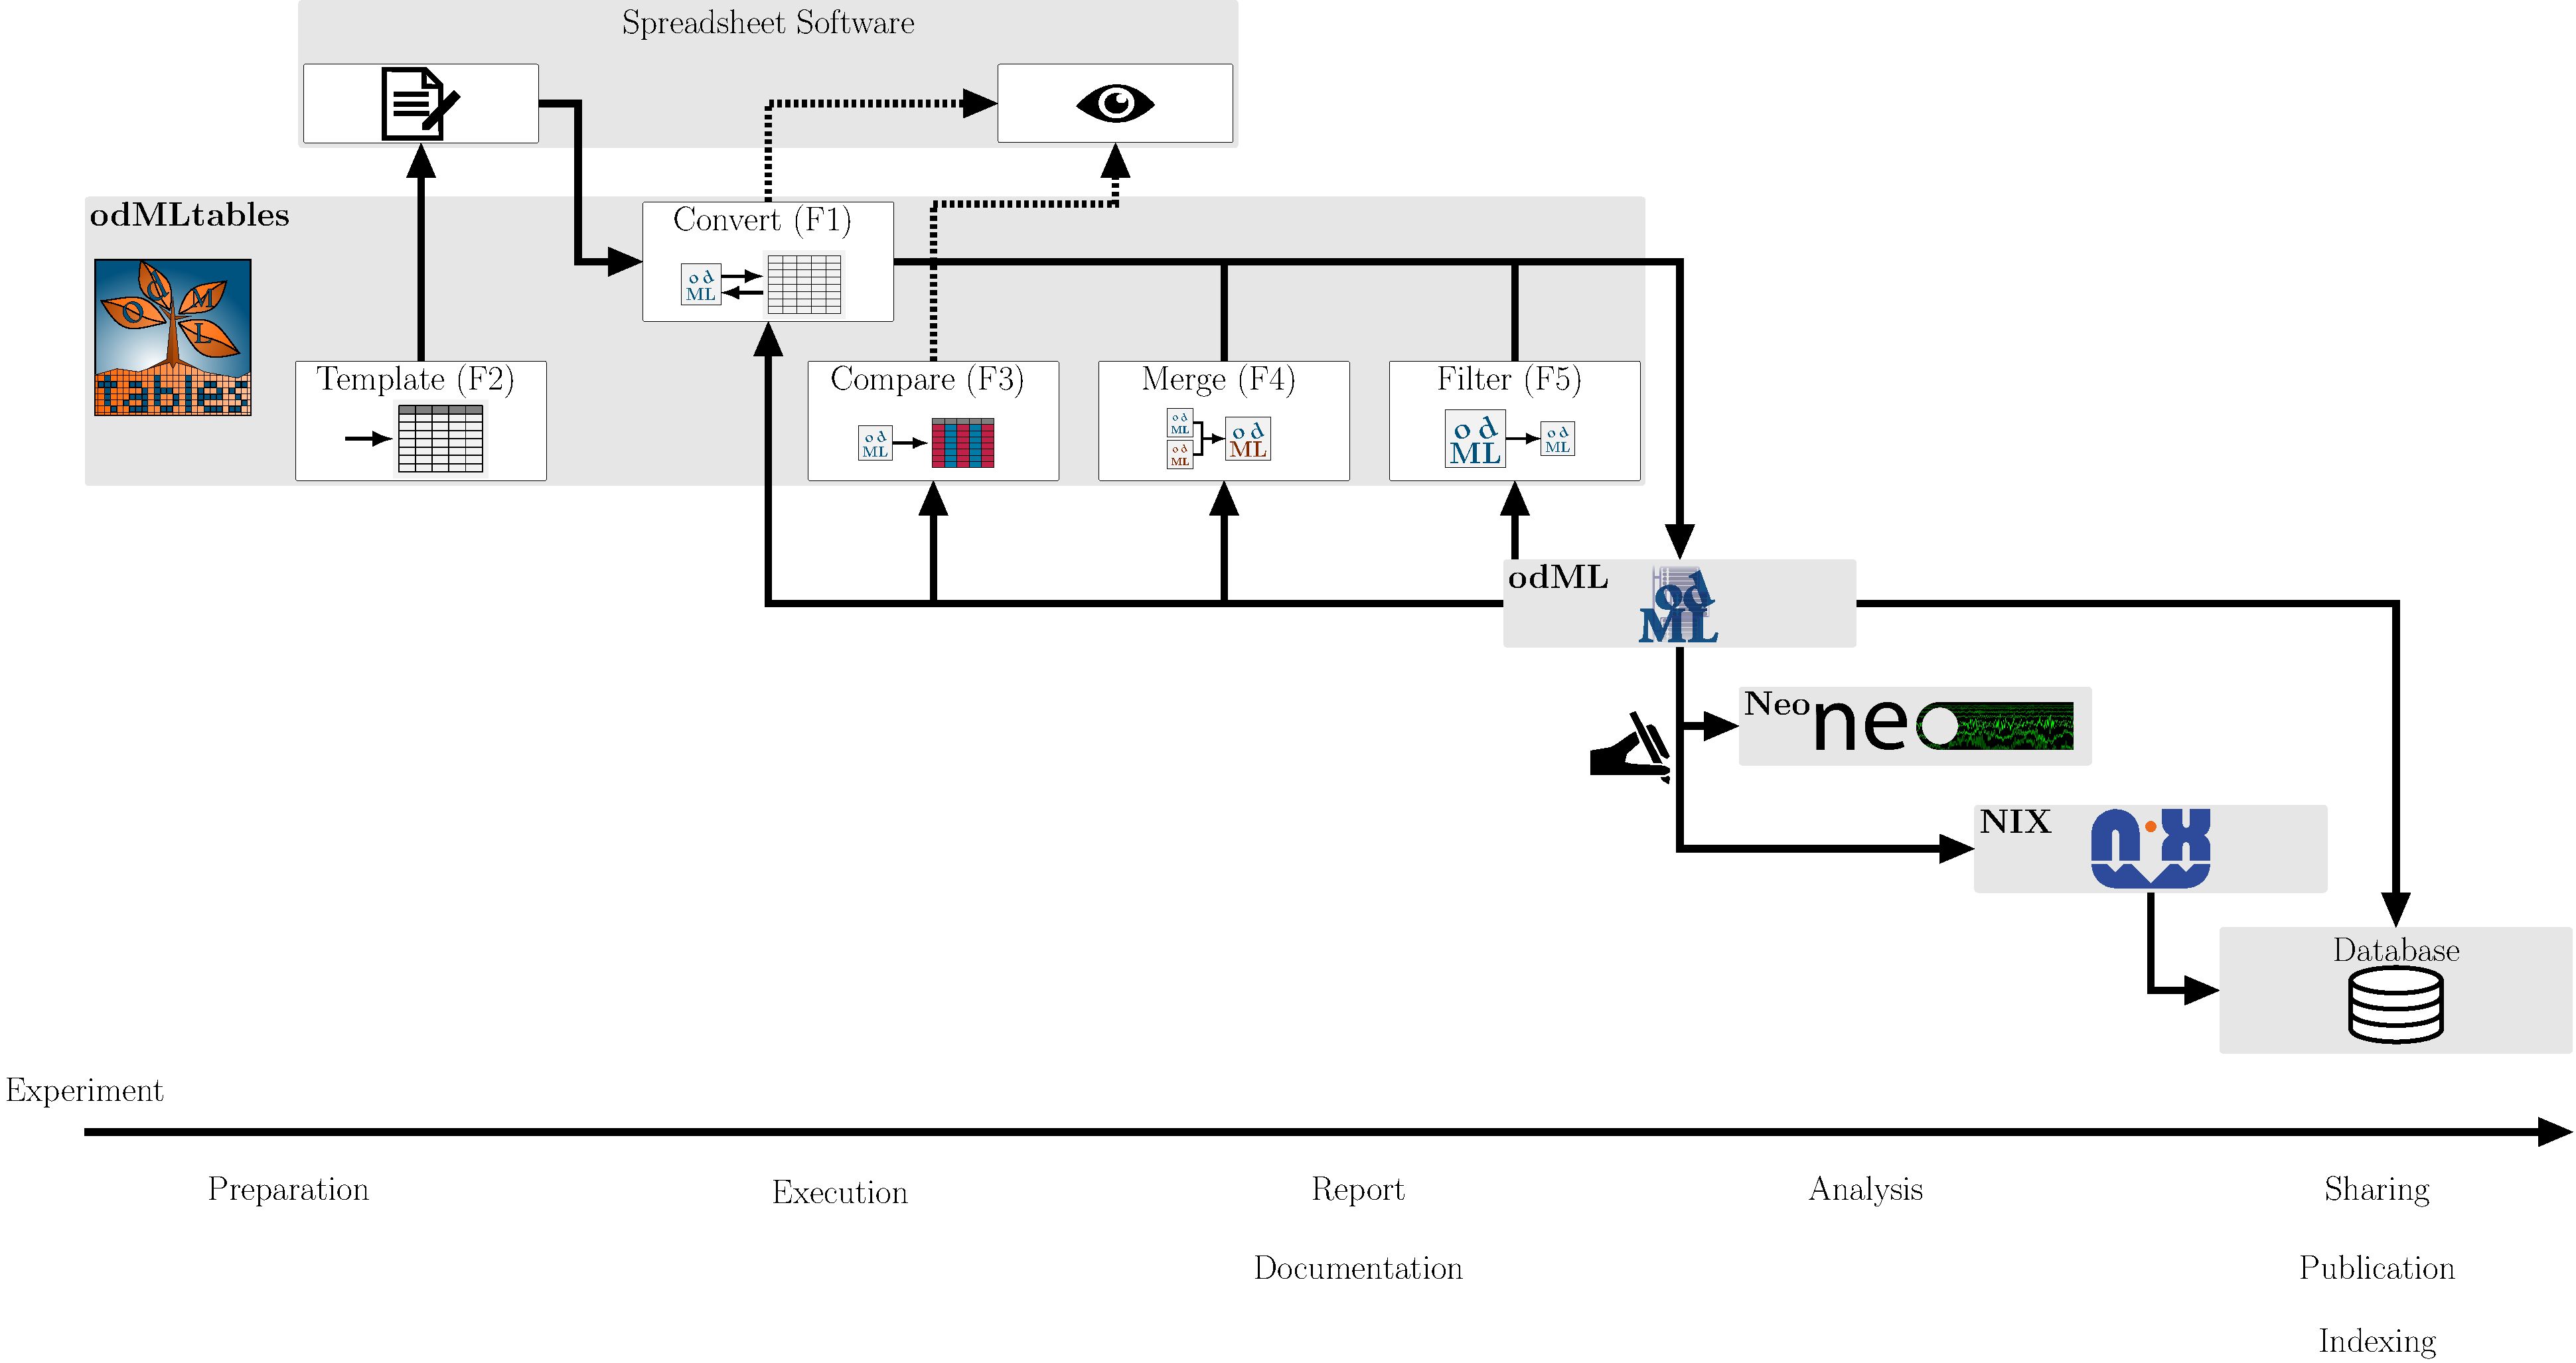
\includegraphics[width=1.0\columnwidth]{figures/odmltables_figures/fig8_global_picture/global_picture.pdf}
\caption[Integrating \software{odMLtables} and other software tools in the different stages of an experiment from preparation to publication]{\label{fig:global_workflow}
\textbf{Integrating \software{odMLtables} and other software tools in the different stages of an experiment from preparation to publication.} During the preparation of an experiment \software{odMLtables} in combination with spreadsheet software is used to develop an experiment specific structure of the metadata collection (templates, \fgenerate{}). During the execution and documentation of the experiment, \software{odMLtables} converts (\fconvert{}) between the tabular and \software{odML} representations. The compare functionality (\fcompare{}) is used to generate overviews of \software{odML} Properties across different Sections of a metadata collection. The filter (\ffilter{}) and merge (\fmerge{}) functionalities are used to create and merge subsets of \software{odML} collections, respectively. For analysis and sharing, data can be represented using the \software{Neo} framework and annotated with metadata from the \software{odML} metadata collection using custom scripts. This combined representation can be saved in a single format using the NIX framework, e.g., to share of data and metadata via a database. In parallel, metadata collections can be incorporated in databases, for example using an export of the \software{odML} to the RDF standard.}
\end{center}
\end{figure}

In recent years, the scientific community has begun to recognize the need for developing workflows that enable rigorous data management not only to ensure reproducibility, but also to expedite research through efficient data sharing among scientists. The principles governing corresponding data management practices are summarized under the FAIR (Findable, Accessible, Interoperable, Reusable) principles \citep{Wilkinson_2016}. The requirement to make data globally findable has lead to the emergence of multiple resources commonly subsurmised under the term ``Knowledge Graph'', referring to a graph-like linkage of metadata through an appropriate ontologies, for example, as done in the Knowledge Graph of the Human Brain Project\footnote{\url{https://www.humanbrainproject.eu/en/explore-the-brain}}. The resource description format, RDF\footnote{\url{https://www.w3.org/RDF}}, is a semantic web technology that provides one possible standard interface to populate such metadata graphs (cf., \cref{fig:global_workflow}). The complexity of creating RDF descriptions from scratch can be simplified by exploiting the functionality of \software{odML} to export RDF schemata from \software{odML} files. In this context, \software{odMLtables} can be incorporated as a bridge to support researchers in easily entering predefined metadata schemata to expose their data records in large-scale Knowledge Graph infrastructures.

\software{odMLtables} is actively developed and a comprehensive documentation including a tutorial is available for release versions on ReadtheDocs\footnote{\url{https://odmltables.readthedocs.io/en/latest}} and the latest version can be obtained from GitHub\footnote{\url{https://github.com/INM-6/python-odmltables/}}. Future developments of \software{odMLtables} include the ongoing embedding of \software{odMLtables} in different neuroscientific data and metadata aggregation workflows, and, as a long term prospect, \software{odMLtables} is planned to become a fully integrated component of the \software{odML} and NIX libraries.


\section{Current code version}
\label{sec:code_version}

\begin{tabular}{ll}
\hline
Code version & 1.0.0 \\
\hline
Permanent link to code/repository & \href{https://github.com/INM-6/python-odmltables}{https://github.com/INM-6/python-odmltables}\\
\hline
Documentation & \href{https://odmltables.readthedocs.io}{https://odmltables.readthedocs.io}\\
\hline
Support & \href{https://github.com/INM-6/python-odmltables/issues}{https://github.com/INM-6/python-odmltables/issues}\\
\hline
Programming Language & \href{https://www.python.org/}{Python}\\
\hline
Dependencies & \href{http://g-node.github.io/python-odml/}{odML}, \href{https://wiki.python.org/moin/PyQt}{PyQt5}\\  
\hline
Research Resource Identifier (RRID) & \href{https://scicrunch.org/scicrunch/Resources/record/nlx_144509-1/SCR_016228/resolver}{SCR\_016228}\\
\hline
Legal Code License  & \href{https://github.com/INM-6/python-odmltables/blob/master/LICENSE.txt}{BSD 3-Clause} \\
\hline
Logo &

\includegraphics[width=0.14\columnwidth]{figures/logos/odMLtables}\\
\hline
\end{tabular}


\todo{Look at github r2g issues to motivate why this is hard to apply to all sessions -> different approach for v4a (inherently cluster based, versioned, snakemake)}

\cleardoublepage
\chapter[Data representation]{Standardized data representations\\- Making data usable}
\label{sec:neo}
% importance of standardization and global organizations 
For widely accepted and utilized and interoperable data storage and usage, as suggested by the FAIR principles for scientific data management \citep{Wilkinson_2016}, it is necessary to agree on common file formats for storage on disc as well as data representations in memory. The agreement on data standards can develop in a i) community driven way by groups of users adopting a format and therefore forming the basis for a general spread of the format or ii) industry defined, by companies or organizations defining a standard. In the context of data storage and representation there are numerous standards already defined and maintained. For example the World Wide Web Consortium\footnote{W3C, \url{https://www.w3.org/}} is an international community, that is coordinating the development and maintenance of open standards to ensure the long-term growth of the internet. This includes e.g. the widely spread scalable vector graphics (svg) format and the Hypertext Markup and Extensible Markup Languages (html, xml, respectively). These standards were developed in a community driven way, and are still continuously improved by working groups\footnote{W3C working groups, \url{https://www.w3.org/Consortium/activities}} (e.g. the svg2 format\footnote{svg2, \url{https://www.w3.org/TR/SVG2/}}).

% why this doesn't cover smaller scientific fields
Standards as they are defined by the World Wide Web Consortium affect millions of users and computer systems. Therefore, the issue of standardization forms a foundation for a working system with this large number of participants. On smaller scales, however, the topic of standardization is not as pressing as individual members are typically able to develop a system, which meets their requirements and often does not require interaction with other systems. At the same time the complexity and specificity of the data and metadata to be represented increases since more detailed information needs to be captured and tracked in a consistent manner. This leads to a an unproportionally high effort required when interacting with other members of the community since the locally established implicit agreements on data storage and handling need to be communicated in addition to the actual data content.

% BIDS as positive example
One way even smaller communities can benefit from standardized data representations from an early stage on is the introduction of standards from the recording system manufacturing side. This situation is more likely to occur if only very few experimental systems exist (e.g. particle physics and the \code{root} format \citep{Brun_1996}) or only few manufacturers produce experimental setups, which simplifies the coordination between these (e.g. medical imaging and the Digital Imaging and COmmunications in Medicine (DICOM) standard\footnote{DICOM, \url{https://www.dicomstandard.org/}}). Based on this, the neuroimaging community managed to extend the standard to coherently organize metadata with data in the Brain Imaging Data Structure\footnote{BIDS, \url{https://bids.neuroimaging.io/}} \citep{Gorgolewski_2016}.

% standards as prerequisite for tool development and vice versa
Standards can emerge from a community or can be established by dominating entities, e.g. in case of a monopoly for hardware production. However, also the development of tools used within and across communities is tightly linked the definition of standards, as these form a prerequisite for interacting with the data. This interaction works both ways: the establishment of standards is important for the development of tools to enable them to get the most information out of the datasets, but also tools can influence the establishment of standards especially in small communities by favouring one format over another and therefore influencing the community preferences. The development of tools applicable across communities requires the prior adoption of global standards, as community internal evolved agreements are typically too diverse to be transferred to other communities to form a basis for a common set of tools. 

% neuroscience: state of the art
A prime example for the delayed recognition for the need of standardization is the development of data formats in the field of electrophysiology. Here specific requirements are needed when recording electrophysiology datasets: The file formats need to be able to support writing of large amounts of data in a streaming fashion, they have to cope with the custom data structure generated by the recording system  and they need to document the parameters used during the recording as minimal metadata. This, together with a number of companies developing ready-to-use solutions for experimentalists led to a multitude of file formats (see also \cref{fig:neo_ios}). All systems permit experimentalists to record data without investing years into the development of a recording system but also typically provide only very few supported output file formats. This again restricts the number of easily applicable analysis methods, as the vendor may provide tools for basic visualization, processing and simple analysis the data, but these are typically not easily extendable nor do they provide a simple programming interface for the implementation of custom analyses. This unnecessarily restricts the scientific questions which can be answered with a particular dataset based on the producer of the hardware system.\\

% neuroshare
A project introducing a common output file format for electrophysiology recording systems is Neuroshare \footnote{Neuroshare, \url{http://neuroshare.org/}}. Version 1.0 was released in 2003 and is a C based library relying on direct-link libraries for the integration with recording systems and providing scripts for the integration in a \software{Matlab} environment. However, neuroshare was only taken up by few vendors of electrophysiology setups, as these are required to provide integration routines for their acquisition system. Additionally, Neuroshare was mainly developed for Windows based systems, making it complicated to use in combination with other operating systems. In 2010 a Python implementation of Neuroshare was introduced\footnote{python-neuroshare, \url{https://github.com/G-Node/python-neuroshare}}, which is currently not maintained.

Since then, multiple projects attempt to tackle this problem from different angles: The Neurodata Without Borders: Neurophysiology\footnote{\software{NWB:N}, \url{https://www.nwb.org/}} (NWB:N) \citep{Teeters_2015} project attempts to define an additional, more generic file format standard aiming to replace a multitude of existing formats. This project was launched in 2014 and a second version was released in 2019 \citep{Rubel_2019}. The project involved multiple scientific laboratories, funding agencies as well as industry partners and provides a fixed set of structures to describe common data encountered in this collaboration. The \software{NWB:N} format is not supported by major recording setup manufacturers and therefore no file format generated by common electrophysiological recording setups. Instead primary recording data need to be converted into the \software{NWB:N} format.
Another project tackling the same problem is the Python package \software{Neo}. \software{Neo} is a spin-off of the \software{Neurotools} toolbox, an attempt to set up a common file format for neurophysiology setups based on Microsoft dynamic-link libraries. It was initiated in 2009 and in contrast to NWB provides a standardized in memory data representation for electrophysiology data without introducing another file format. Therefore it bridges the gap between available electrophysiology file formats and forms the basis for a number of visualization, preprocessing and analysis tools. By interfacing to a large number of file formats \software{Neo} is the ideal tool for implementing flexible data management workflows independent of the particular file format of the original data files. In addition, it provides also flexibility in the range of software tools that can be used for further data processing as it interfaces with various tools that cover diverse requirements of data processing, visualization and analysis. In the following we will introduce \software{Neo} in more detail and provide example scripts for application of \software{Neo} for handling electrophysiology datasets.



\section{The \software{Neo} Python package}
\software{Neo}\footnote{\software{Neo}, \url{http://neuralensemble.org/neo}, RRID:SCR\_000634} \citep{Garcia_2014} is an open-source Python package for representing electrophysiology data in working memory. It offers interfaces for reading various electrophysiological proprietary and open file formats and represents the data in a generic way (\cref{fig:neo_uml,fig:neo_ios}). Thus it forms the bases for a number of open software tools: The electrophysiology analysis toolkit\footnote{Elephant, \url{http://neuralensemble.org/elephant}, RRID:SCR\_003833} for analysis of spiking activity and local field potentials, OpenElectrophy\footnote{OpenElectrophy, \url{http://neuralensemble.org/OpenElectrophy}, RRID:SCR\_000819}, SpykeViewer\footnote{SpykeViewer, \url{https://spyke-viewer.readthedocs.io}} and Ephyviewer\footnote{Ephyviewer, \url{https://ephyviewer.readthedocs.io}} for visualization, Tridesclous\footnote{Tridesclous, \url{https://tridesclous.readthedocs.io}} for online and offline spike sorting, NeoAnalysis\footnote{NeoAnalysis, \url{https://github.com/neoanalysis/NeoAnalysis}} \citep{Zhang_2017} for rudimentary visualization and analysis, NetworkUnit \footnote{NetworkUnit, \url{https://github.com/INM-6/NetworkUnit}, RRID:SCR\_016543} for validation testing of spiking networks. Related packages are \software{NiBabel}\footnote{NiBabel, \url{https://nipy.org/nibabel}, RRID:SCR\_002498}, a comparable package for neuroimaging file formats and \software{MNE}\footnote{MNE, \url{https://martinos.org/mne}, RRID:SCR\_005972} an Python package for MEG and EEG analysis and visualization.

\begin{figure}[]
    \centering
    \includesvg[width=\textwidth,pretex=\relscale{0.8}]{./figures/neo07_schema.svg}
    \caption[\software{Neo} 0.7 object structure]{\software{Neo} 0.7 object structure. Figure modified from \url{https://github.com/neuralensemble/python-neo}.}
    \label{fig:neo_uml}
\end{figure}


\begin{figure}[hbtp]
    \centering
    \includestandalone[mode=image|tex, width=\textwidth, obeyclassoptions=true]{./figures/neo_ios_and_tools}
    \caption[Neo embedding]{\software{Neo} embedding. \software{Neo} 0.7. supports a number of file formats for reading (light blue) and writing (dark blue). Many of the supported formats can be read in a improved fashion, permitting for more efficient memory usage (black frames).  Neo provides an interface for many advanced tools for visualization, simulation, analysis and data storage.}
    \label{fig:neo_ios}
\end{figure}

The two main features of \software{Neo} are 1) the interfacing to many different file formats, by providing reading capability for numerous proprietary formats and writing capability to selected open formats and 2) the standardized representation of electrophysiology data as a basis for further visualization and analysis steps. Using these features of \software{Neo} is typically used either as conversion tool from specialized to more generic formats or as run time data representation for further processing.


\begin{figure}[hbtp]
    \centering
    \software{Neo} 0.3 architecture
    \includesvg[width=\textwidth]{./figures/neo_architecture03.svg}
    \caption[\software{Neo} 0.3 architecture]{\software{Neo} 0.3 architecture. \software{Neo} represents electrophysiology signals in data objects such as \code{AnalogSignal}s, \code{AnalogSignalArray}s, \code{IrregularlySampledSignal}s, \code{SpikeTrain}s and \code{Spike}s, whereas the latter two optionally include information about waveform data for each spike. Additional supplementary information describing the timing during the recording can be provided using \code{Event}s and \code{EventArray}s or \code{Epoch}s and \code{EpochArray}s to mark time points or durations during the recording, respectively. All above described data objects are put into relation by container objects, such as \code{Segment}s (grouping all data objects simultaneous in time), \code{Unit}s (grouping \code{SpikeTrain}s and \code{Spike}s across time), and \code{RecordingChannel}s and \code{RecordingChannelGroup}s (grouping \code{AnalogSignal}s \code{IrregularlySampledSignal}s and \code{Unit}s, \code{AnalogSignalArray}s and \code{RecordingChannel}s, respectively). The top level container is a \code{Block} linking to \code{Segment}s and \code{RecordingChannelGroup}s. Figure from \url{https://neo.readthedocs.io/en/0.3.3}.}
    \label{fig:neo_architecture03}
\end{figure}


\begin{figure}[hbtp]
    \centering
    \includesvg[width=\textwidth]{./figures/neo_architecture07.svg}
    \caption[\software{Neo} 0.7 architecture]{\software{Neo} 0.7 architecture. \software{Neo} represents electrophysiology signals in data objects such as \code{AnalogSignal}s, \code{IrregularlySampledSignal}s and \code{SpikeTrain}s optionally including information about waveform data for each spike. Additional supplementary information describing the timing during the recording can be provided using \code{Event}s or \code{Epoch}s to mark time points or durations during the recording, respectively. All above described data objects are put into relation by container objects, such as \code{Segment}s (grouping all data objects simultaneous in time), \code{Unit}s (grouping \code{SpikeTrain}s across time) and \code{ChannelIndex}es (grouping \code{AnalogSignal}s \code{IrregularlySampledSignal}s and \code{Unit}s). The top level container is a \code{Block} linking to \code{Segment}s and \code{ChannelIndex}es. Figure modified from \url{https://github.com/neuralensemble/python-neo}.}
    \label{fig:neo_architecture07}
\end{figure}


\begin{figure}[hbtp]
    \centering
    \includesvg[width=\textwidth]{./figures/neo_architecture_future.svg}
    \caption[Proposed \software{Neo} architecture]{Proposed \software{Neo} architecture. The proposed \software{Neo} architecture preserves all objects from \software{Neo} version 0.7 except for \code{ChannelIndex}es and \code{Unit}s. These are replaced by \code{Group} and \code{View} objects, which a more generic, but still customizable way of organizing data objects. \code{View} objects can mask data objects by linking to a subset of the contained data (e.g. a single trace of an \code{AnalogSignal}. This linking is unidirectional, preventing complex dependencies involving data objects. \code{Group}s are capable of linking to any kind of data objects or \code{View} of data objects. The required specificity is provided by the different \code{mode}s of a \code{Group} object. These limit to the connected objects to a specific type and number, wherefore a \code{Group} can e.g. be used instead of a \code{Unit} object. \code{Group}s can also link to other \code{Group} objects to provide higher level organization of the data.}
    \label{fig:neo_architecture_future}
\end{figure}

\subsection{Feature updates and current development}
The \software{Neo} version 0.3 was released in 2014 \citep{Garcia_2014}. Since then the software has been extended to be compatible with more data formats, the object model has been revised for better usability and the implementation has been improved for performance. In the following we describe the enhancements introduced between version 0.3 (\cref{fig:neo_architecture03}) and version 0.7 (\cref{fig:neo_architecture07}).

\paragraph{Interfaces to file formats}
\software{Neo} 0.7 is supporting additional file formats for reading, such as Axograph, OpenEphys, Stimfit, Kwik, Nix, Igor, Nest, Neuralynx, NSDF and BCI2000. The capabilities for reading the Axon, Blackrock, Brainvision, Brainware, Elphy, Intan Matlab structures, Neuroshare, Plexon, Spike2, Tdt, NeuroExplorer, Neuralynx, Igor, Elan, Micromed, RawMCS, WinWCP formats have been improved. Reading and writing capabilities have been improved for Nix and Pickle formats. PyNNText and PyNNNumpy formats are no longer supported. A new code design for readers has been implemented and the majority of readers has adjusted accordingly to enable improved loading performance and loading of subsets of data (RawIO implementation). 
\paragraph{Object structure and usability}
The code has been modularized for more flexibility and maintainability, and a large number of unittests have been added. The object structure has been restructured for user friendliness and to boost performance by implementing sets of similar data entities in single objects instead of using individual data objects for each data entity (removal of dedicated array versions of data classes). A new relational container object \code{Channel\_Index} was introduced to simplify the representation of logical relations between data objects replacing \code{RecordingChannel} and \code{RecordingChannelGroup} objects. Consistent deep copy functionality has been added for all data objects and additional internal consistency checks have been added. A new type of custom annotation mechanism has been added, which is designed to capture custom annotations in the same dimension as the data (array annotations). For the installation additional option were introduced, depending on the required file formats which need to be supported. The code style has been adjusted to follow the PEP8 guideline\footnote{Python Enhancement Proposal 8, \url{https://www.python.org/dev/peps/pep-0008}}\citep{PEP8StyleGuideforPythonCode_}. Support for Python 2.6 was dropped and consistent support for Python 3 was introduced.


\paragraph{Outlook}
Practical application of \software{Neo} confirmed an improved usability for version 0.7. The described data objects facilitate data access and performance and the combination of \code{Block} and \code{Segment} objects as container objects provides easy to use access to the data. However, the concept of \code{ChannelIndex} objects is covering too many aspects of relations between data at once: 1) grouping data objects, 2) masking data objects (selection of a subset of data within a data object) and 3) annotating individual samples within data objects. The last aspect has been moved to the individual data objects, by introducing array annotations. 

% groups and views
For future versions, the splitting of \code{ChannelIndex} objects into two separate objects (\code{Group}, \code{View}) responsible for grouping and masking is planned. A \code{Group} object will be able to link different types of data objects, depending on its configuration. For example a \code{Group} object resembling a physical electrode will be able to link to a single \code{AnalogSignal} and multiple \code{Unit} objects. A \code{View} object can be used to refer to a subset of the data stored in a data object (e.g. a single recording trace within an \code{AnalogSignal}). This view can be used instead of a data object in any relation and will provide utility functionality to provide a sliced version of the actual data object.

%linking
Another topic of discussion is the linking between \software{Neo} objects. Up to the current version 0.7 all links between \software{Neo} objects can be established bidirectional. However, the bidirectionality of the linking is not inherently guaranteed, since the generation of a link does not automatically generate a backward link between \software{Neo} objects. Introducing automatic bidirectional linking would guarantee bidirectional linking, but might complicate the set up of a \software{Neo} structure e.g. when reading a data file. There are different approaches possible to circumvent these problems: i) The use of only unidirectional links from higher level to lower level objects (top to bottom). This approach would still provide most of the functionality commonly used. ii) The implementation of a validation framework, which can on request check if a provided \software{Neo} object structure is fully linked including consistent bidirectional links. A suggested model implementing the first of the two suggestions is presented in \cref{fig:neo_architecture_future}. Here links from \code{View}s and \code{Group}s towards data objects are unidirectional, therefore preventing cyclic links across the complete \software{Neo} structure.

%Imaging data
Spiking activity of individual neurons can not only be recorded using sharp electrodes, but also  from multielectrode array recordings (MEA) and calcium image recordings \citep{Kelly_2007, Shew_2010}. To support the usage of \software{Neo} also for imaging data an extension of \software{Neo} by two additional object types is planned: the \code{ImageSequence} object will capture sequences of regularly sampled images and is therefore closely related to the \code{AnalogSignal} as it contains the same type of data, but also captures the spatial relation between different pixels (traces). A second object relevant for image handling is a \code{RegionOfInterest} object, which is used to spatially mask a specific part of a stack of images. The \code{RegionOfInterest} can implemented as special case of a \code{View}. Support for \code{ImageSequence}s also requires capabilities to read imaging data formats, which will be added subsequently.


\subsection{\software{Neo} object structure}
% data vs container objects, general attributes: name, description, file\_origin
\software{Neo} objects can be separated into two types: data objects, describing basic recording data in combination with minimal metadata and container objects, providing the structural framework for the relation between the data objects (\cref{fig:neo_uml}). In general, all \software{Neo} objects have three optional arguments to provide custom information about the captured data: 1) The \code{name} attribute can be used to label the object and can be used for simple data filtering and selection. 2) The \code{description} attribute is intended to provide a human readable, detailed, 1-2 sentence description for the data contained / grouped by the \software{Neo} object. The \code{file\_origin} is can be used to describe the origin of the data, e.g. the original recording filename or simulation script. In addition to \code{name}, \code{description} and \code{file\_origin}, all \software{Neo} objects can capture additional custom information in form of an \code{annotation} dictionary. This dictionary can contain arbitrary data in all basic Python data types as well as \code{datetime}, \code{date}, \code{time}, \code{timedelta} in arbitrary structures build from lists, dictionaries, tuples or \software{Numpy} arrays without any restrictions on the shape of these objects.


\paragraph{Data objects}
Data objects are based on \software{Numpy} arrays \citep{Walt_2011} for efficient computation on large datasets. In addition, \software{Neo} objects are aware of physical quantities by using the \software{Quantities} package \citep{Dale_} (\cref{fig:neo_uml}).



% Continuously Sampled Signals
\software{Neo} provides data objects to capture regularly as well as irregularly sampled continuous signals in \code{AnalogSignal} and \code{IrregularlySampledSignal} objects, respectively. Both objects rely on a 2 dimensional \software{Quantities} (\software{Numpy}) array capturing the basic data signal, whereas the first dimension describes the time and the second dimension different signal traces. For \code{IrregularlySampledSignal}s time information is captured in a second separate \software{Quantities} array, sharing the first dimension with the signal array. For \code{AnalogSignal}s this in implemented in a more compact fashion by storing only the sampling rate (\code{sampling\_rate}) and the starting time point of the recording (\code{t\_start}). A \software{Quantities} array containing the time values corresponding to the data point can be generated on request via the \code{times} attribute of the \code{AnalogSignal}.
% Time series data
For time series data \software{Neo} provides a \code{SpikeTrain} object, capturing the data in a \code{times} attribute. Additionally the start and stop times of the data acquisition are essential for the interpretation of the data, these are provided as mandatory \code{t\_start} and \code{t\_stop} scalar \software{Quantities} parameters. Optionally, a \code{SpikeTrain} object can also capture snippets of regularly sampled continuous signal around each time point in the waveform attribute. This links to a 3 dimensional array, capturing the time, spike ID and recording channel dimensions of the waveforms. The \code{SpikeTrain} attribute \code{sampling\_rate} is used to capture the corresponding sampling information as in the \code{AnalogSignal} case. To relate the waveform snippets with the time series data the \software{Quantities} scalar \code{left\_sweep} defines the constant offset between the time series data and the corresponding waveform snippet.
% Events and Epochs
A different type of time series data is non-neuronal time series which describe specific time points or durations during the recording of neuronal activity. These might be control signals of the experiment, e.g. trial start times, behavioral events of the subject, e.g. a the time in which a button was pressed. For the description of time series data \software{Neo} provides \code{Event} objects, capturing the data in a one dimensional \software{Quantities} array (\code{times} attribute) together with a string array of the same shape (\code{labels} attribute) providing labels to the individual time points. To represent extended periods of time, \software{Neo} offers \code{Epoch} objects having the same attributes as \code{Event}s, and in addition a one dimensional \software{Quantities} array of durations with the same shape as the main time series data.

% Array annotations
All of the above mentioned data objects consist of a main \software{Quantities}-wrapped \software{Numpy} array with one or more dimensions. One of the latest features introduced in \software{Neo} is to implement a second kind of annotation mechanisms on this. The annotations of an object always refer to the object as a whole. However, in many use cases annotations have been used to provide details about the individual data samples by containing arrays, which share some dimensions with the main data samples. For example \code{AnalogSignals} which contain more than one recording trace are frequently annotated with list providing detailed information about the individual recording channels, e.g. the identity of the channel or the particular filter settings. However, when modifying the shape of the original data, these annotations can not be updated in an automatic fashion since they were user defined and didn't follow a fixed schema. Since \software{Neo} version 0.7.0 all data objects have an additional feature \code{array\_annotation}s, which fills this gap by providing an annotation mechanism for capturing sample based annotations, i.e. annotation entries with the same length as the main data dimension. These \code{array\_annotations} are automatically adjusted when the shape of the main data is modified, e.g. by slicing the data in the time axis or extracting a single signal trace from an \code{AnalogSignal}.

% Lazy loading
The \code{Neo} 0.7 release also features a standardized way of optionally loading specific parts of the data on request. This is of advantage when dealing with datasets which are large in comparison to the available memory. The new \code{lazy} feature permits to generate the complete \software{Neo} structure (\cref{fig:neo_architecture07}), but substituting all data objects with proxy objects, which feature the same attributes and links as classic data objects, but do not contain the actual data. For accessing the data a \code{load} mechanism is provided which loads the requested parts of the data and provides them in a separate classic data object not linked to the main \software{Neo} structure. Using the \code{lazy} mechanism large datasets can be processed chunk wise without requiring large amounts of memory.

\paragraph{Container Objects}
% Block and Segment
\software{Neo} container objects provide the structural relations between \software{Neo} data objects. The base object for a dataset is a \code{Block} object, containing everything related to the dataset. The \code{Block} object can link to a number of \code{Segments} and \code{ChannelIndex} objects which can be used to organize data objects according to their timing, spatial relation or custom grouping aspects, e.g. grouping the data objects by the signal quality of the contained data. \code{Segment} objects are intended for grouping objects which share the same time frame, e.g. simultaneously recorded \code{AnalogSignal}s and \code{SpikeTrain}s (\cref{fig:neo_architecture07}).
\code{SpikeTrain}s from different \code{Segment}s that are considered coming from the same source (neuron) can be linked across \code{Segments} via \code{Unit} objects.
% Units and ChannelIndexes
A \code{Unit} object again can be grouped together with \code{AnalogSignal}s and \code{IrregularlySampledSignal}s in a \code{ChannelIndex} object. In addition to the grouping functionality, a \code{ChannelIndex} object also provides an additional labeling functionality for child \code{AnalogSignal}s via the \code{channel\_ids} and \code{channel\_names} attributes. These consist of one dimensional integer and string arrays labeling the individual traces of the attached continuous signals. Via the mandatory attribute \code{index} a selection of the traces within the linked continuous signals can be done. However, this requires a consistent ordering of recording traces within all linked continuous signals of a \code{ChannelIndex}.
All container objects provide utility functions to facilitate access and selection of data objects. This is implemented in the form of a \code{filter} method, which returns a list of \software{Neo} objects based on a combination of object type, attribute and annotation constraints.




\section{\software{Neo} usage examples}
In the following we demonstrate in three practical examples how \software{Neo} can be used to load data from different file formats in a memory efficient manner, access and select data, annotate and filter data according to custom metadata added and save data in an open source format.

\subsection{Loading \& visualization}
Loading data in \software{Neo} is implemented in two stages: First initialization of the reader (IO) and second reading of the \software{Neo} structure. For readers implemented in the standardized manner (\cref{fig:neo_ios}, black frame) you need to provide the filename of the dataset to load. This will generate an \code{io} object providing functionality to load the data into a \software{Neo} structure. Depending on the file format either a \software{Neo} \code{Block} or a \software{Neo} \code{Segment} can be loaded using the \code{read\_block} or \code{read\_segment} method of the \code{io} object.

In this example, the published dataset described in \cref{sec:data} is used for demonstrating the loading of electrophysiology data into the \software{Neo} structure (\cref{code:neo_visualization}). Data were previously downloaded from GIN\footnote{\url{https://gin.g-node.org/INT/multielectrode_grasp}} and continuous as well as sorted spiking data are loaded using the \software{Neo} \code{BlackrockIO} class. This IO provides standardized access to the data, permitting lazy loading of \software{Neo} objects (cf. \cref{code:neo_visualization} line 10f). Here the \software{Neo} filter functionality is used to select all \code{SpikeTrain}s which have an annotation key \code{'channel\_id'} and the corresponding value of the user requested channel index (\code{selected\_channel}, line 13). In the next step, the corresponding \code{AnalogSignal} trace is extracted by finding the \code{AnalogSignal} with a corresponding entry in the \code{array\_annotation}s with key \code{channel\_ids} and extracting the \code{id} of the corresponding trace (line 15-18). Finally, the analog and spiking data of 10 seconds of recording are loaded into memory via the \code{load} mechanism of the respective data objects and returned by the \code{load\_single\_channel\_data} function (line 19-22).

\begin{codeenv}[hbtp]
\inputminted[linenos,tabsize=2,breaklines, fontsize=\scriptsize]{python}{figures/code_visualize_data.py}
\caption[Data loading and visualization with \software{Neo}]{Loading data into the \code{Neo} framework and visualization using the Matplotlib package. Required packages are imported (line 1-4) and two main functions are defined for loading and visualization of the \software{Neo} structure: \code{load\_single\_channel\_data} and \code{plot\_data}. The first one requires the location of the datasets and the selected channel to plot as command line arguments (line 9). Here, the dataset is opened using the \code{BlackrockIO} in \code{lazy} mode and the user-specified channel is selected and loaded into memory together with the spiking activity (lines 7-22). The second function visualized a given \code{AnalogSignal} together with a list of \code{SpikeTrain}s using the \software{Matplotlib} package (line 25-40). Finally both functions are run subsequently using command line parameters for dataset and channel specifications. For the resulting plot see
\cref{fig:demo_visualization}}.
\label[codelisting]{code:neo_visualization}
\end{codeenv}

\begin{figure}[hbt]
    \centering
    \includesvg[width=\textwidth]{./figures/i140703-001.svg}
    \caption[Data visualization example]{Visualizating of the activity recorded on a single electrode. A single trace of an AnalogSignals contains the voltage samples of a recording electrode (blue). The corresponding threshold crossing events are split into three different \code{SpikeTrain} objects and time stamps are marked as vertical lines with a \code{Unit} specific offset (orange, green, red).}
    \label{fig:demo_visualization}
\end{figure}


The visualization of a single \code{AnalogSignal} trace together with spiking activity from multiple \code{SpikeTrain}s is implemented in the \code{plot\_data} function. This requires the corresponding data objects as input as well as a location to store the final scalable vector graphics plot (line 25). Here, \software{Matplotlib} \citep{Hunter_2007} is exploited to visualize the electrophysiological data (line 30 \& 34-38). Correct scaling of the signals and automatic generation of axis labels is ensured by the inherent use of the \software{Quantities} package within \software{Neo} (line 28-31, 34-37). The resulting plot is exported to the scalable vector graphics (svg) format for storage in a flexible, memory efficient and scalable manner. Finally, user specific setting are extracted from command line parameters and both functions are executed sequentially to generate a visualization of a single recording trace and corresponding spiking activity.


\subsection{Annotation of data with metadata from \software{odML}}
Annotations are a key feature of the generic \software{Neo} structure to provide the necessary customizations to be used for a specific dataset. Standard annotations are a feature of all \software{Neo} objects and can be accessed via the \code{annotation} attribute. In addition, \software{Neo} data objects also provide a more specific type of annotation mechanism, namely \code{array\_annotations} which act in the same manner as regular \code{annotations} but are directly coupled to the dimension of the underlying data. This permits to store metadata which are linked to individual data entries and handle them in an automatic way when manipulating the data object. This example demonstrates how to access and modify regular and array annotations using a metadata collection in the odML format.

\cref{code:neo_annotation} demonstrates two aspects of \software{Neo} annotations: firstly annotation access via the object attributes \code{annotation} and \code{array\_annotation} and secondly the generation of (array) annotations. The resulting script output is shown in \cref{code:neo_annotation_print}. The dataset is loaded in the same manner as in \cref{code:neo_visualization} and \code{annotations} and \code{array\_annotations} of selected objects are printed using the \code{print\_annotations\_example} function. The resulting printout shows the different levels of annotations, which are automatically generated by \software{Neo} when loading a dataset from the \code{Blackrock} format. Annotations on the \code{Block} level provide general information about the recording session, whereas \code{SpikeTrain}s carry very specific metadata about the identity of the object and its spike sorting classification.

An example for \code{array\_annotations} is provided for an \code{AnalogSignal}. \code{AnalogSignal} objects provide the most metadata as they describe all recording traces they contain individually (see \cref{code:neo_annotation_print} line 15-33). Here the \code{AnalogSignal} contains 96 recording traces and all array annotations have a matching length of 96. The annotated information covers the identity of the electrodes ('channel\_ids' and 'channel\_names', line 16f) and identity within the recording system ('connector\_ID' and 'connector\_pinID', line 19f) as well as signal processing parameters for signal filtering and spike extraction (line 21-30). Here the keys consist of a combination of the file type affected (nsx/nev), the filter border (high/low), the general parameters (freq/energy\_threshold/dig(itization)\_factor/waveform\_size) and filter parameters affected (corner/order/type). In addition, a human readable description as well as information about the originating file is provided ('description', 'nsx' and 'file\_origin', line 18, 31f). All \code{array\_annotations} will automatically be adjusted when the underlying data object is modified via \software{Neo} functions, e.g. via slicing in time.

The second part of the example script (\cref{code:neo_annotation}, line 28ff) demonstrates the generation of additional (array) annotations by loading a metadata collection in the odML format, extracting relevant information for the interpretation of an \code{AnalogSignal} and adding this information to the \code{AnalogSignal} as array annotation. First, an odML file is loaded using the Python \software{odML} library (line 31) and all \code{Sections} describing electrodes are extracted to load a mapping between the Blackrock channel \code{ID}s provided by the recording system and the spatially ordered \code{ConnectorAlignedID}s (line 32f), which are defined in order to indicate an electrode's spatial position easily. In the next step, the existing Blackrock \code{ID} array annotations of an \code{AnalogSignal} are used to generate the corresponding array of \code{ConnectorAlignedID}s using the previously extracted mapping b(line 36f). Finally, the new ids are added as a new array annotation to the \code{AnalogSignal} using the \code{array\_annotate} mechanism (line 38).

\begin{codeenv}[hbtp]
\inputminted[linenos,tabsize=2,breaklines, fontsize=\scriptsize]{python}{figures/code_annotate_data.py}
\caption[Annotation access and editing with \software{odML} and \software{Neo}]{Annotation access and editing with \software{odML} and \software{Neo}. Required packages are imported (line 1) and three functions for printing \code{annotations} and \code{array\_annotations} are defined (line 3-25). \code{pretty\_print\_dict} provides functionality for displaying individual dictionary items in separate lines (line 3-6). \code{print\_annotations} uses the previous function to print based on the \code{mode} keyword the \code{annotations} or \code{array\_annotations} of a given \software{Neo} object. \code{print\_annotation\_example} prints a selection of \code{annotations} and \code{array\_annotations} from a \software{Neo} block structure. The function \code{generate\_annotations\_from\_odml} extracts metadata information about the mapping of different types of \code{id}s from an \code{odML} file and annotates the corresponding \code{AnalogSignal} (line 27-37). Finally, all functions are demonstrated based on a command line specified data- and metadataset (\code{data\_location} and \code{odml\_filename}, line 40-45). The generated annotations are confirmed via a final call of \code{print\_annotations} (line 46f).}
\label[codelisting]{code:neo_annotation}
\end{codeenv}

\begin{codeenv}[hbtp]
\inputminted[linenos,tabsize=2, fontsize=\scriptsize, style=friendly]{cucumber}{figures/i140703-001_annotations.txt}
\caption[Output of \cref{code:neo_annotation}]{Output of  \cref{code:neo_annotation}. Listed are the automatically generated annotations of example \software{Neo} objects as extracted from \code{Blackrock} recording files. On the \code{Block} level these are dealing with general information about available files and interruptions in the recording process. For \code{SpikeTrain}s there is information provided about the identity and classification of the \code{Unit} the \code{SpikeTrain} was assigned to. For \code{AnalogSignal}s there are arrays describing the attributes of the individual electrode traces. This includes information about the electrode identities (\code{channel\_ids}), mappings of contacts within the recording system (\code{connector\_ID}s, \code{connector\_pinID}s) and the applied filter and threshold settings for signal preprocessing and spike extraction.}
\label[codelisting]{code:neo_annotation_print}
\end{codeenv}


The generated array annotations are displayed by printing the complete array annotations of the \code{AnalogSignal} again, resulting in \cref{code:neo_annotation_print} line 43ff. Here, the new key 'connector\_aligned\_ids appears containing the corresponding spatially organized ids of the recording electrodes.

With array annotations and annotations, \software{Neo} now offers a mechanisms to provide custom information for \software{Neo} objects as a whole, but also for subsets of data contained by \software{Neo} objects. With these annotation mechanisms it is now possible to directly add \software{odML} content to \software{Neo} objects on multiple levels of the data organization. However, this annotations are not automatically generated yet, since there is no mechanism assigning data in the \software{Neo} structure and metadata in the \software{odML} structure. Due to the generality of \software{Neo} and \software{odML} structure the is no generic assignment strategy between the two structures possible, but these relations need to be captured explicitly using an extended framework.


\subsection{Saving data \& format conversion}
\label{sec:nix_format}
Being able to store intermediate preprocessing steps or analysis results in a persistent manner is important for making workflows reproducible. \software{Neo} provides the option to store data in plain ASCII, KlustaKwik \citep{Hazan_2006}, Nix \citep{Stoewer_2014}, binary Matlab, Neuroscience Simulation Data Format (NSDF) \citep{Ray_2016}, binary Python pickle and a custom binary format, see also \cref{fig:neo_ios}. In this example we focus on the Nix format as it provides the most versatile data storage. Nix is based on an hdf5 \citep{TheHDFGroup_1997} backend which provides the flexibility of fast and memory efficient access for large datasets. In addition, Nix is designed to capture data as well as metadata, providing the opportunity to unify both in a single file and add links between relevant metadata and the corresponding data. 
This example demonstrates the conversion of the dataset used already in previous examples from the \code{Blackrock} format to the \software{Nix} format. Furthermore, it showcases the addition of metadata from the \code{odML} format to the same file and the extraction of the data from the \software{Nix} file.
\cref{code:neo_saving} provides four functions for the back and forth conversion of files in the \software{Neo} and \software{odML} format to the \software{Nix} format (line 4-24). These functions are mostly based on the open-source \software{nix-odML-converter} library \footnote{\url{https://github.com/G-Node/nix-odML-converter}}. This library can be used for simple command line conversion between \software{Nix} and \software{odML}. Here we demonstrate the usage of the Python interface, permitting a more flexible approach to conversion parameters (e.g. filenames, write modes).
We demonstrate the merging of the data together with the metadata into a single \software{Nix} file using the first two functions (\cref{code:neo_saving} \code{save\_neo\_to\_nix} and \code{save\_odml\_to\_nix}). The last two functions deal with the extraction of the corresponding information of the individual components from the \code{Nix} file (\cref{code:neo_saving} \code{load\_odml\_from\_nix} and \code{load\_neo\_block\_from\_nix}).

With the capability of the \software{Nix} format to capture data as well as metadata in a combined fashion both modalities can be comprehensively stored in a common framework. Integrating both modalities in the \software{Nix} format is easy since \software{Neo} supports the writing of data in the \software{Nix} format and metadata can be supplemented using the \software{nix-odML-converter}.

\begin{codeenv}[hbtp]
\inputminted[linenos,tabsize=2, fontsize=\scriptsize]{bash}{figures/code_saving_data.py}
\caption[Saving data and metadata to \software{NIX}]{Saving data and metadata to \software{NIX}. Required packages are imported (line 1f) and four functions for the conversion between \software{Neo} and \software{odML} on the one side and \software{Nix} on the other side are defined (line 4-24). The main part of the script (line 26ff) first extract command line specified parameters (location of the dataset and \software{odML} and \software{Nix} filenames to be used) and loads the datasets from the \code{Blackrock} format. Next, the \software{Neo} block in converted to the \software{Nix} format (line 32) and the complete metadata collection is added from an \software{odML} file (line 33). Finally, we demonstrate how to extract the corresponding information again from the \software{Nix} format using the \code{load\_odml\_from\_nix} and \code{load\_neo\_block\_from\_nix} functions (line 36f). Please note that the execution time of this code highly depends on the size of the dataset, since for sequentially all parts the complete dataset will is loaded into memory.}
\label[codelisting]{code:neo_saving}
\end{codeenv}


\section{Comparison of \software{Neo} and \software{NWB:N}}
The \software{NWB:N} format \citep{Teeters_2015} is an alternative approach to \software{Neo} for handling of electrophysiology data. In contrast to \software{Neo} it specifies a new file format instead of providing interfaces to existing formats. More precisely, \software{NWB:N} provides a modular framework for the capture of specific electrophysiology modalities. %https://pynwb.readthedocs.io/en/stable/overview_software_architecture.html
It is accompanied by a number of canonical schema (type) for capturing specific types of data, e.g. behavioural and time series data, imaging recordings, extra and intracellular electrophysiology recordings as well as optogenetic stimulation and optical physiology. Custom schema can be specified to capture data modalities not covered by the set of canonical schema.  % https://nwb-schema.readthedocs.io/en/latest/
This makes the \software{NWB:N} format on the one side more generic than the \software{Neo} structure, since it permits the implementation of custom schema specifications, but on the other side also more restrictive, because existing schema specifications are very specific and can not be reused in a slightly different context. Also implementation of a custom schema specification extensions in \software{NWB:N} requires additional background knowledge of the experimenter about the underlying organization of the \software{NWB} package and the time and effort of implementing such a format. %https://nwb-schema.readthedocs.io/en/latest/format_description.html#extending-the-format
For \software{Neo} the approach is different: the underlying object structure is  generic to automatically cover most of the electrophysiology data and the experiment specificity is introduced via the annotation and array annotation mechanism. This implies that the user only has to understand the \software{Neo} objects once and can reuse the knowledge also in different experimental contexts.
\software{Neo} can deal with most of the available electrophysiology file formats and will be extended to cover calcium imaging data in the future. For \software{NWB:N} there are very limited conversion tools available to convert from specific \software{Matlab} structures and custom formats to the \software{NWB:N} format. %https://github.com/NeurodataWithoutBorders/exp2nwb  https://github.com/NeurodataWithoutBorders/mat2nwb https://github.com/NeurodataWithoutBorders/nwbn-conversion-tools
An interface for the support of additional formats exists, but format converters are in an early development stage. At this point \software{NWB:N} could benefit from integrating \software{Neo} to gain basic support for many electrophysiology formats.
\software{NWB:N} has reference implementations in Python as well as Matlab, suiting most of the neuroscientists, whereas \software{Neo} is only implemented in Python, focusing on non-commercial availability of electrophysiology analysis software.


\section{Summary}
We introduced the \software{Neo} Python package designed for standardized and efficient representation of electrophysiological data. We presented the development of the package since the original publication and depicted the main features and flexibility of the package in three small usage examples. Finally we provide a concise comparison to the recent \software{NWB:N} format and highlight the strengths of the software packages.
Using the \software{Neo} package provides a sound foundation for organizing research data according to the FAIR principles as \software{Neo} i) makes data accessible by supporting the conversion from various file formats to the standardized \software{Neo} data representation, ii) is an open, freely available and software package and iii) it makes data interoperable by providing a formal, accessible and broadly applicable basis for data representation. In addition \software{Neo} is supporting the \software{Nix} file format, which is fulfilling additional FAIR principles. These are i) making the data within the file format findable by using globally unique identifiers for data and metadata objects, ii) permitting the annotation with rich metadata as extensive metadata collections can be stored, iii) connecting data and metadata in a formal way by storing links between data and metadata objects, iv) being an open and free \& interoperable framework.
Additional aspects of the FAIR principles, like provenance tracking of the data and metadata, require the embedding of \software{Neo} and \software{Nix} in a data and metadata pipeline or workflow.



\clearpage
\chapter[Workflow management]{Workflow management\\- A new approach for research data and metadata management}
\label{sec:workflows}
The long process that starts from the generation of data, and ends in a scientific publication, can be separated into many individual steps. These subdivision may be coarse, like the separation only of experiment and subsequent analysis. Or they may be very fine, as each individual operation, and substeps within, may constitute and be implemented in independent processes.

Workflow management is the concept to organize these individual steps. The granularity of the steps to manage highly depends on the complexity of the tasks and the diversity of the processing steps. A common and generic example forming such a workflow management system (WMS) is a queuing system used in cluster computing such as \software{slurm}\footnote{slurm workload manager, \url{https://slurm.schedmd.com/}} or  \software{torque}\footnote{torque resource manager, \url{http://www.adaptivecomputing.com/products/torque/}} and \software{maui}\footnote{maui cluster scheduler, \url{http://www.adaptivecomputing.com/products/maui/}}. Here users submit a number of, in the simplest case, independent jobs (computing steps) which are then scheduled and distributed to suitable compute resources depending on the requested and available resources. This is a simple example, because the individual processing steps typically do not depend on each other and only the required amount of resources and time needs to be taken into account when organizing the execution. Already with these systems, it is possible to implement more complex scenarios, e.g. by defining an order of execution via dependency statements for individual jobs.

In this chapter we apply the concept of workflow management to solve the data and metadata management issues identified in \cref{sec:scidata_shortcomings}. A systematic workflow approach for data and metadata management supports the rigorous implementation of the FAIR principles, since the automation of processing steps relies to some extend on FAIR principles, i.e data should to have a unique identifier and should be organized in a structured fashion using standardized tools. Additionally, the implementation of a data and metadata workflow increases the reproducibility of the processing steps, as these are documented and provenance information can be tracked for each step of the workflow. Workflow management is suited to tackle the issues we identified in \cref{sec:scidata_shortcomings}, since it is designed to coordinate interdependent steps of a process as they occur in the data and metadata pipeline of the Reach-to-Grasp project. In the following, we present available WMSs and identify requirements for the applicability in the context of scientific projects in general as well as for Reach-to-Grasp and similar projects in particular.

For scientific projects like the Reach-to-Grasp experiment described in \cref{sec:data} there are dependencies between individual steps of the process from data acquisition to publication (see \cref{fig:scidata_metadata_pipeline,fig:scidata_reachgraspio_diagram}). The workflow management concept has been applied in a number of scientific fields like genomics or imaging data. In these fields a systematic approach to data processing and analysis is required and feasible, since they are dealing with large and numerous datasets which exceed manual monitoring or processing power \citep[e.g.][]{Palm_2010}.
For these and other disciplines, there are a number of platforms and tools available to implement pre \& post processing as well as analysis processing steps: Galaxy\footnote{Galaxy, \url{https://galaxyproject.org}, RRID:SCR\_006281}, an  open, web-based platform providing bioinformatics tools and services for data intensive genomics research; VisTrails\footnote{VisTrails, \url{https://www.vistrails.org}, RRID:SCR\_006261}, an open-source scientific workflow and provenance management system that provides support for simulations, data exploration and visualization; Taverna\footnote{Taverna, \url{https://taverna.incubator.apache.org}, RRID:SCR\_004437}, a scalable, open source \& domain independent tool for designing and executing workflows;  GenePattern\footnote{GenePattern, \url{http://www.broadinstitute.org/cancer/software/genepattern}, RRID:SCR\_003201}, a genomics analysis platform that provides access to hundreds of tools for gene expression analysis, SNP analysis, flow cytometry, RNA-seq analysis, and common data processing tasks; Renku\footnote{Renku, \url{https://datascience.ch/renku}}, an online software platform for reproducible and collaborative data science including workflow management aspects; Terra\footnote{\url{https://terra.bio/}}, a scalable platform  for biomedical research for data analysis and collaboration; Ugene \citep{Okonechnikov_2012} a multi platform open-source software for molecular biology; Luigi\footnote{Luigi, \url{https://luigi.readthedocs.io}}, a Python based tool for building complex pipelines of batch jobs; Airflow \footnote{Airflow, \url{https://airflow.apache.org/index.html}}, a platform programmatically author, schedule and monitor workflows; pinball\footnote{pinball, \url{https://github.com/pinterest/pinball}}, a scalable workflow manager with scheduling capability implemented in JavaScript and Python; make, a basic build automation tool available since 1976 with multiple implementations (e.g. gnumake\footnote{gnumake, \url{https://www.gnu.org/software/make/}}) and snakemake\footnote{Snakemake, \url{https://snakemake.readthedocs.io/en/stable/}, RRID:SCR\_003475}, a Python based language and execution environment for make-like workflows. 

In simple and straightforward projects, one may use plain bash scripts to coordinate the sequential execution of the individual steps of a workflows, mimicking a WMS. However, once the situations grows more complex, the same issues arise as discussed for the Reach-to-Grasp metadata pipeline (\cref{sec:scidata_shortcomings}): the bash script would form a monolithic script, trying to cover all possible dependencies between individual scripts resulting in overly complex code. Additionally, the script could only be executed all at once, without taking into account which steps of the workflow are actually required due to updates in the underlying sources files.

Scientific projects, such as the Reach-to-Grasp project presented in \cref{sec:data}, can benefit greatly from a structured workflow approach. However, the development of the workflow should in the best case smoothly integrate with the existing scientific tools and approaches used in the project. In the following, we discuss a number of essential features of a WMS, which are generally required in scientific projects. The WMS should 
\begin{quote}
\begin{description}
 \setlength{\itemsep}{5pt}
 \setlength{\parskip}{0pt}
 \setlength{\parsep}{0pt}
 \item[slim] not introduce unnecessary additional computational overhead
 \item[easy]  not require expert knowledge to implement and configure a workflow
 \item[standalone] not introduce additional unnecessary dependencies to other projects and programming languages
  \item[visual] be able to generate a visual overview of the workflow for inspection and debugging purposes
  \item[debuggable] be easy to debug
  \item[active] be actively supported
  \item[open] be open source and freely available\\
\end{description}
\end{quote}
Furthermore, we identify additional, more specific requirements in the context of the Reach-to-Grasp and similar projects. Here, the WMS should
\begin{quote}
\begin{description}
 \setlength{\itemsep}{5pt}
 \setlength{\parskip}{0pt}
 \setlength{\parsep}{0pt}
 \item[Python] inherently support Python as many of the existing scripts are implemented in Python
 \item[integration] integrate well with existing scripts as the existing code base should not depend on the WMS.
 \item[flexibility] provide the flexibility to implement processing steps based on bash (for usage of external tools, e.g. for spike sorting)
 \item[HPC] support local workflow execution as well as the usage of compute clusters by supporting common queuing systems
\end{description}
\end{quote}

The general requirements for a slim and standalone WMS with only minimal overhead already excludes the majority of WMSs listed above as these provide a multitude of features like web applications that are not required in the context of the scientific projects presented here. This rules out Galaxy, Renku, Terra as these are web based WMSs based on a webinterface for user interaction. Ugene and GenePattern focus on very different domains (molecular biology \& genomics, respectively) and provide a multitude of tools for these domains, which are not required here. Pinball and Taverna are java based which is not used in the context of the Reach-to-Grasp or related projects.  In addition, Taverna is a highly developed workflow system with 3500 services available, which surpasses our requirements. Airflow and Luigi are Python-based WMSs that rely on a custom workflow definition in a Python script, which requires tool-specific knowledge for implementation and maintenance of the workflow. VisTrails is Python based as well, but relies on a graphical user interface for the workflow definition, thereby making the implementation of complex workflows cumbersome. Make is a well established tool for the organization of build processes and is therefore available on all operating systems. It has been shown that scientific workflows for quality assurance can be implemented using make \citep{Askren_2016}. However, the workflow definition via make is laborious as well due to a limited utility functionality. Here, snakemake offers a hybrid solution of make and Python. The workflow definition is implemented in a make concept, but Python functionality can be used to facilitate the definition of the workflow within the rigid structure provided by make. Since Python is already the language of choice in the Reach-to-Grasp project, snakemake does not introduce any additional language dependencies and is therefore our tool of choice in order to demonstrate the usage of WMSs in the context of data and metadata management in scientific projects.


\section{Workflow management tools - Snakemake}
\label{sec:snakemake}
In this section we discuss snakemake as a WMS, as it is domain independent, slim and easily integrates with Python based projects, e.g. to the Reach-to-Grasp and related projects (\cref{sec:data}).

Snakemake is a generic workflow management tool derived from the build automation tool make combined with Python features \citep{Koster_2012}. It is available as bioconda\footnote{\url{https://anaconda.org/bioconda/snakemake}} and PyPi package\footnote{\url{https://pypi.org/project/snakemake}}. We consider the so far latest version $5.5.4$ here.

We demonstrate the basic features of snakemake based on two minimal workflow examples. The first one (\cref{code:workflows_simple_snakefile}) demonstrates the basic concept of make and the ability of snakemake to define steps in the workflow in which the involved filenames are not known beforehand. The second, more complex workflow (\cref{code:workflows_python_snakefile}) demonstrates the integration of snakemake with Python and showcases its capabilities of flexibly deducing rule dependencies and parameters of individual workflow steps.

The description of individual steps of a workflow within snakemake is closely related to Make: A processing step is defined via its input and output files (\cref{code:workflows_simple_snakefile}, line 11 and 12). The core of a rule is the instruction how to generate the output files based on the input files. Here snakemake offers multiple options based on direct execution of Python scripts or bash scripting. Bash scripts offer the most flexibility and are marked with the \code{shell} keyword (\cref{code:workflows_simple_snakefile}, line 13). Within executed shell command references to the input and output files can be used via Python based reformatting of the command before execution. E.g. in \cref{code:workflows_simple_snakefile}, line 13 the filename specified by the input of the rule \code{simple\_copy\_rule} (line 11) is automatically copied to the filename specified by the output of the rule by using \code{\{input\}} and \code{\{output\}} in the shell command. The same concept can be used to formulate snakemake rules in a more flexible fashion. E.g. in \cref{code:workflows_simple_snakefile} a set of flexible rules is introduced, which use an additional wildcard \code{\{filename\}} to be able to generate and copy not only files with filename \code{'file.md'}, but any markdown file. Here, the value of the variable \code{\{filename\}} is only determined during the execution of the workflow. Therefore, the same rule can be used multiple times within a workflow with different wildcard parameters. Hereby, the value of the wildcard is determined recursively by the required output file.

The dependencies between snakemake rules are evaluated based on required files. By default snakemake uses the first rule within a \code{Snakefile} as main rule and tries to execute this rule. Alternatively snakemake can be called with a filename as an argument. In this case snakemake attempts to build the requested file based on all available rules, thereby matching in and output files of rules and checking the availability of basic input files. For this purpose snakemake generates an acyclic directed graph of rule dependencies (e.g. see \cref{fig:python_demo}) and infers all wildcard parameters from this. In case multiple rules can be used for generation of the same file a rule priority order can be be defined (\cref{code:workflows_simple_snakefile}, lines 1-3). Snakemake only executes rules and creates or overwrites files if the output files of a rule do not exist or the input files have a more recent modification time stamp than the output files. This guarantees that the output files of a snakemake workflow are always based on the most recent version of input files and at the same time minimizes the computational overhead, since only required or outdated files are generated.


\begin{codeenv}
\textbf{Snakemake header}
\inputminted[firstline=1, lastline=3, linenos,tabsize=2,breaklines, fontsize=\scriptsize]{bash}{figures/workflows/simple_demo.snakefile}
\begin{multicols}{2}
\textbf{Simple rules}
\inputminted[firstline=5, lastline=13, linenos,tabsize=2,breaklines, fontsize=\scriptsize]{bash}{figures/workflows/simple_demo.snakefile}
\columnbreak
\textbf{Flexible rules}
\inputminted[firstline=15, lastline=23, linenos,tabsize=2,breaklines, fontsize=\scriptsize]{bash}{figures/workflows/simple_demo.snakefile}
\end{multicols}
\caption[Minimal snakemake example workflow]{Minimal snakemake example workflow. The workflow consists of two rules: i) generation of a markdown file (.md) and ii) conversion to a text file by plain copy of the content into a file with .txt extension. Two versions of each rule are implemented, demonstrating snakemake features at different complexities: The simple version of the rule handles filenames explicitly (left), whereas the flexible version of the rule is using wildcards to handle filenames (right). To resolve ambiguities between the two versions of the rules, we define a rule priority order in the first lines of the snakemake file.}
\label[codelisting]{code:workflows_simple_snakefile}
\end{codeenv}


\begin{codeenv}
\begin{multicols}{2}
\textbf{Snakefile}\\
\inputminted[firstline=1, lastline=40, linenos,tabsize=2,breaklines, fontsize=\scriptsize]{bash}{figures/workflows/python_demo.snakefile}
\columnbreak
\textbf{Environments}\\
\textbf{plotting\_environment.yaml}
\inputminted[linenos,tabsize=2,breaklines, fontsize=\scriptsize]{yaml}{figures/workflows/envs/plotting_environment.yaml}
\textbf{data\_generation\_environment.yaml}
\inputminted[linenos,tabsize=2,breaklines, fontsize=\scriptsize]{yaml}{figures/workflows/envs/data_generation_environment.yaml}
\textbf{config.yaml}
\inputminted[linenos,tabsize=2,breaklines, fontsize=\scriptsize]{yaml}{figures/workflows/config.yaml}
\end{multicols}
\caption[Snakemake example workflow for data generation and plotting]{Snakemake example workflow for data generation and plotting. The workflow consists of three rules, for data generation, data visualization and specification of the all output files of the workflow. The first two rules can be executed in dedicated conda environments, specified via the \code{conda}-directive and are shown on the right. The workflow uses a configuration file (Snakefile, line 1, \code{config.yaml}), specifying the format for storing \software{Neo} structures. This specification is also used to provide a constraint for wildcards with the name \code{data\_ext}, which resolves ambiguities between the data generation and visualization rule. The rule \code{all} is by default executed when snakemake is run. It specifies two required output formats of the workflow. For the visualization of the workflow diagram when running the \code{all} rule, see \cref{fig:python_demo}.}
\label[codelisting]{code:workflows_python_snakefile}
\end{codeenv}


Snakemake rules can be executed in dedicated, containerized environments. For Python workflows, snakemake supports conda environments on a per-rule level. Here, the conda environment can be defined via a \code{yaml} file specifying the conda (and PyPi) dependencies (see \cref{code:workflows_python_snakefile} Snakefile, line 16 and 23 and environments). When no cached version of the environment exists or the \code{yaml} environment definition was updated, snakemake builds the environment using conda.

\cref{code:workflows_python_snakefile} demonstrates a more complex workflow using two generic Python scripts (\cref{code:workflows_python_scripts}) . The first script generates data based on the \software{Neo} package, whereas the second script visualizes any data accessible via \software{Neo} using the Python \software{Matplotlib} package. These scripts are implemented to be used as standalone scripts, and require arguments from the command line indicating the filename. Additionally, they do not rely on a fixed data file format, but support any format supported by the  \software{Neo} framework. This, in combination with the explicit definition of the required conda environments in form of \code{yaml} files makes the scripts highly flexible and generic, such that they can be easily reused in different contexts and projects. Furthermore, the snakemake implementation of the workflow keeps the generality of the code by providing flexibility in the used data format, which is defined via an additional configuration \code{yaml} file, and the usage of wildcards for flexible handling of filenames. The resulting snakemake workflow as well as the output visualization of the randomly generated data can be seen in \cref{fig:python_demo}.

\begin{figure}
%     \begin{multicols}{2}
    \begin{minipage}[t]{0.4\textwidth}
    \textbf{A}\\
    \includesvg[width=\textwidth, pretex=\relscale{0.8}]{figures/workflows/python_demo_escus}
    \end{minipage}
    \begin{minipage}[t]{0.6\textwidth}
%     \columnbreak\\
    \textbf{B}\\
    \includesvg[width=\textwidth]{figures/workflows/data}\\
    \end{minipage}
    %     \end{multicols}
 \caption[Snakemake example workflow for data generation and plotting]{Snakemake example workflow for data generation and plotting. The workflow diagram (A) and resulting plot (B). The workflow consists of two rules of which the \code{plot\_data} rule is executed twice with different parameters to generate the final plot in two file formats (\code{ext:svg}, \code{ex:png}, respectively). Different rules are color coded and the rule name is indicated at the top of each node.  The command line parameters of the scripts are indicated below the rule name. The frame style (solid/dashed) indicates if this rule needs to be run to generate a final output file. In this example, the data file was already generated, wherefore snakemake would not rerun this rule unnecessarily (dashed box). The arrows indicate the dependencies between the rule executions. Rules at the top need to be executed first, since they generate output files that are required as input for the subsequent rules executions.}
\label{fig:python_demo}
\end{figure}


\begin{codeenv}
\begin{multicols}{2}
\textbf{Data generation}
\inputminted[linenos,tabsize=2,breaklines, fontsize=\scriptsize]{python}{figures/workflows/generate_data.py}
\columnbreak
\textbf{Data visualization}
\inputminted[linenos,tabsize=2,breaklines, fontsize=\scriptsize]{python}{figures/workflows/plot_data.py}
\end{multicols}
\caption[Standalone Python scripts used in \cref{code:workflows_python_snakefile}]{Standalone Python scripts used in \cref{code:workflows_python_snakefile}. The two scripts for data generation and visualization contain generic functions, relying on command line parameters to provide the arguments for the function calls (lines 21-24 and lines 18-21, respectively). The \textbf{data generation} is split into two functions, one for generation of the \software{Neo} structure (\code{generate\_neo\_data}) and one for saving the \software{Neo} structure to disc (\code{save\_neo\_block}). The first function generates a \software{Neo} \code{Block} containing a single \code{AnalogSignal} with randomly generated data (lines 4-12). The second function receives a generic \software{Neo} \code{Block} and saves it in the format specified by the provided filename (lines 16-19). If the script is executed from the command line, the input parameter \code{filename} is extracted from the command line arguments and both functions are executed consecutively, passing the \software{Neo} \code{Block} from one function the next (lines 21-24). The \textbf{data visualization} uses the same concept as the data generation. Here the two internal functions are loading a \software{Neo} block from the specified data source filename (\code{load\_neo\_block}, lines 4-7) and visualize the first \code{AnalogSignal} of a given plot, saving the result in a requested filename (\code{plot\_analogsignal}, lines 9-16). Both functions are called if the script is called from the command line and the two parameters specifying the data location as well as the output plot filename are extracted from the command line arguments.
}
\label[codelisting]{code:workflows_python_scripts}
\end{codeenv}

In addition to the features demonstrated in the example scripts, snakemake integrates well distributed storage concepts, such as Google Cloud Storage\footnote{Google Cloud Storage, \url{https://cloud.google.com/storage/}}, Dropbox\footnote{Dropbox, \url{https://www.dropbox.com}}, or the secure shell protocol (SSH). Remote file sources are declared in the header of the snakemake file and individual files can be referenced from these sources in the same manner as local files. Besides access to remote files, snakemake also integrates with high-performance compute clusters by supporting common queuing systems such as the slurm workload manager\footnote{slurm, \url{https://slurm.schedmd.com}}. Here, a configuration file can be used to specify the cluster job parameters on a rule-level, permitting detailed resource management.

\paragraph{Summary}
We presented the application of basic snakemake features based on two examples demonstrating the modularization of a workflow into individual rules and their file-based dependency handling. We highlighted the flexibility of this approach by introducing wildcard based filename handling and explained the snakemake dependency graph. We provided examples of generic standalone Python scripts for seamless integration into snakemake rules and demonstrated advanced configuration features of the workflow via additional configuration files and wildcard constraints. We introduced additional features for integration of remote files and cluster usage.
The presented features make snakemake our tool of choice for the implementation of scientific workflows, as it provides a domain-independent and slim option for workflow definition which integrates well with existing scripted data processing steps.


\section{Practical application}
Snakemake has been applied in a variety of fields and projects. Many of the provided examples and tutorials are set in the field of genomics\footnote{\url{https://snakemake.readthedocs.io/en/stable/getting_started/examples.html}}$^,$\footnote{\url{https://snakemake.readthedocs.io/en/stable/tutorial/basics.html}}. Here we present a workflow design in the context of the Vision-for-Action project, a successor project of Reach-to-Grasp.

\subsection{The Vision-for-Action project}
The Vision-For-Action project builds on top of the Reach-to-Grasp project as it extends the investigation of motor control only to the interaction of motor and visual activity. The involved continuous integration of both visual input and motor control demand a more sophisticated experimental task protocol. The experimental hardware is a Real-time visuomotor behavior and electrophysiology recording (RIVER) setup, which utilizes a \software{Blackrock} system in order to record neuronal activity, as described for the Reach-to-Grasp experiment (\cref{sec:data}). For more details, we refer to \citet{deHaan_2018,deHaan_2018a}. The recording system additionally encompasses an eye tracking as well as a hand movement control system and a complex task design, which includes the sequential pointing to up to six targets. To the current date, only a single monkey was recorded in the Vision-for-Action setup.

\paragraph{The task}
In the Vision-for-Action experiment a monkey is positioned in front of a horizontal, semi-transparent mirror, onto which a white dot corresponding to its hand position below the mirror, is projected (\cref{fig:river_setup}). The monkey is trained to initialize a task by moving the hand cursor into the area of a central, illuminated target. After a waiting period of $200ms$, during which the monkey has to stay in the center, the central target is deactivated and, depending on the task type, one or multiple of 6 peripheral targets are illuminated. To receive a reward, the monkey has to deactivate all illuminated targets by moving the hand cursor into the each of the targets. Depending on the task additional targets appear upon the deactivation of a previous one. Two classic task types are currently implemented: The landing task, in which the monkey is presented a sequence of three peripheral targets, which he has to deactivate by staying in each of the targets for $100ms$ resulting in mostly straight hand movements to the target. In the drawing task, the monkey is presented multiple targets at once and can chose an order and route to deactivate these. In this task type the monkey only needs to touch the target with the hand cursor. It was observed that this typically causes very curved hand movement trajectories.


\paragraph{The setup}
The RIVER setup consists of three components recording different modalities: i) the neural activity via a \software{Blackrock} system described in the context of the Reach-to-Grasp experiment ii) the eye movement via a an EyeLink tracking system and iii) the arm movement via a Kinarm motorized exoskeleton (\cref{fig:river_setup}).

As in the Reach-to-Grasp experiment, neural activity is recorded using a Utah array recording device. In the Vision-for-Action experiment, however, additional to a single Utah array implanted in motor cortex, four smaller arrays are implanted in visual cortex.  $96$ active recording electrodes are present in motor cortical area M1 and premotor cortex. Furthermore, $32$ active electrodes, arranged in a $6\times6$ grid, are located in each of the vision-related cortical areas V1, V2, 7a and DP. The neural activity is recorded by two parallel setups (see \cref{fig:river_setup} purple boxes). This includes two separate connectors implanted contralateral to the Utah arrays and ipsilateral to the active hand of the monkey. Each of the two connectors is connected to a separate headstage including a neural signal amplifier, digitizer and converter. The signals of each headstage are then optically transmitted to one of two real-time Neural Signal Processors (NSPs) which perform online signal processing (filtering, spike extraction and sorting). In the next step, the processed neuronal signals of each NSP are transmitted to a corresponding offline Cerebus computer for writing to disc and monitoring by the experimenter.

The active arm of the monkey is attached to a Kinarm system, which can be used to track and interfere with the monkey's movement (\cref{fig:river_setup} green boxes). The Kinarm restricts the hand movement to a horizontal plane below the working space of the monkey and can be used to exert forces onto the monkey's arm. Online feedback of the hand location is provided visually in form of a circular white cursor in the working space.

The gaze position of the monkey is tracked using an EyeLink system (\cref{fig:river_setup}, blue boxes). To be able to record the gaze position, the monkey's head is placed in a plastic head mask, restricting large head movements and providing access to the reward system. The gaze direction is inferred from a video signal that shows the position of the pupil and the corneal reflection of an infrared light source. The raw eye direction signal is processed online into the final eye position sin gal through the Kinarm real-time system. This conversion depends on the exact location of the monkey's eye with respect to the camera and light source and therefore needs to be calibrated frequently to ensure a stable gaze position recording. For a detailed description of the configuration mechanism and procedure, see \citet{deHaan_2018}.

All online tracked signals, neuronal, Kinarm as well as gaze, are input to at least one of the  two NSPs. This results in two sets of \software{Blackrock} files as original data files generated by the RIVER setup.

The experiment control is implemented as a Simulink model on the Kinarm real-time computer. This model coordinates the experiment using a Stateflow description of the experimental task and by generating corresponding event codes encoding the state of the system. The event codes are unique and globally defined in a generic manner using a $16$ bit code. Of the $65536$ possible codes, $1246$ codes are reserved for generic experimental events like a trial start or the beginning of a trial metadata sequence. This leaves $64290$ unused codes, providing sufficient flexibility for future extensions of the scheme. Each event code can contain metadata further specifying properties of a specific event, e.g. the maximum time range the monkey has to reach the next target before the trial is aborted. For robustness, all event codes come in pairs of two, bracketing the metadata information in a start and end bracket. The globally defined experimental codes follow a systematic scheme grouping events based on their first digit in six categories: 'Experiment Metadata', 'Trial Metadata', 'Screen Related', 'Exoskeleton Related', 'Other', 'Behaviour Related' and 'Error'. For more details on the global encoding of metadata see \citet{deHaan_2018a}.
For a specific task implementation used in the experiment, a mapping of the globally defined codes to the task specific metadata is defined. This approach permits the global use of generic event codes in the recorded data which at the same time is capable of capturing all task specific metadata. The global event codes generated by the Simulink model, together with hand and gaze location information, are forwarded to the Blackrock system and saved together with the neuronal signals.

\paragraph{Synchronization}
It is essential for the interpretation of the data and their coherent recording from three different systems that these share a common time frame. The RIVER setup produces two sets of \software{Blackrock} files since all other signals are integrated online during the recording. The two NSPs provide a feature, which permits to synchronize the two systems upon start. To ensure continued synchrony between the two systems, the two NSPs receive common input from the Kinarm system, which can be used offline for validating the common recording time frame.

\paragraph{Data and metadata files}
The RIVER setup saves multiple signals in parallel, as described in the following. Two sets of \software{Blackrock} recording data files are recorded: one containing neural signals from motor and the other from visual cortical areas in the \code{ns6} format. In addition, both datasets contain partially identical behavioral signals for the hand, arm and gaze position in the \code{ns2} format (\cref{tab:v4a_recording_files}). Furthermore, the position of the active target is stored with a $1kHz$ sampling rate as well as the synchronization signals which are shared between the two NSP / Cerebus systems.



\begin{sidewaysfigure}
 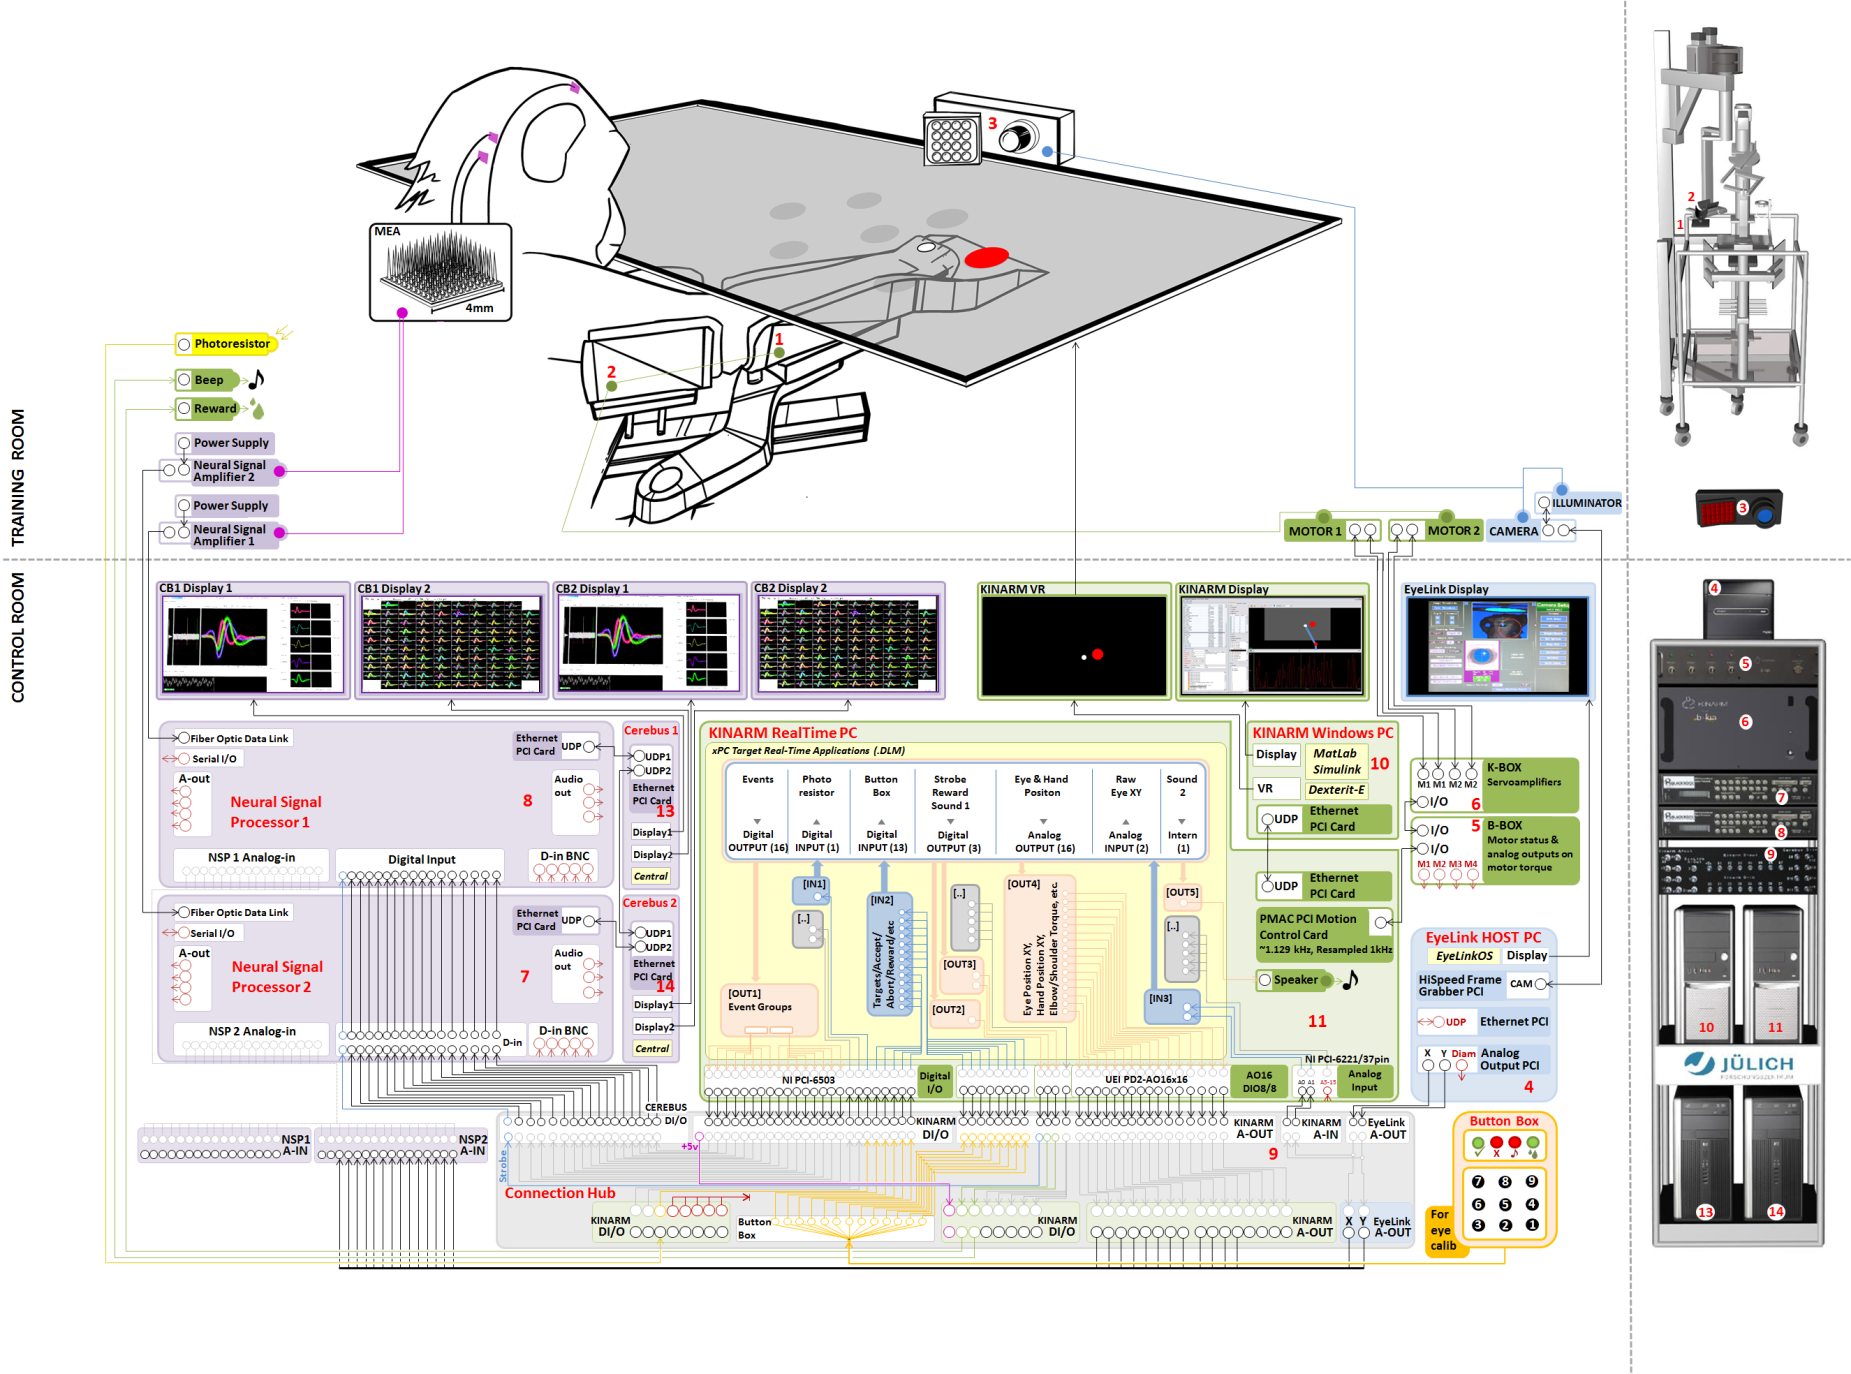
\includegraphics[width=0.8\textwidth]{figures/workflows/river_setup_hardware}
 \caption[The RIVER setup]{The RIVER setup including schematic of hardware components and signal flows. Depicted are the monkey task setup (top right), the recording system and signal flows (bottom left), the monkey chair and Kinarm (top right) and the recording hardware rack (bottom right). Figure from \citet{deHaan_2018a}.}
 \label{fig:river_setup}
\end{sidewaysfigure}


\begin{table}[]
\centering
\begin{tabular}{ll}
\hline
file format & content                                               \\ \hline \hline
*.ccf       & cerebus configuration                                 \\ \hline 
*.nev       & digital events                                        \\
            & \textbullet~ unsorted spike times                      \\
            & \textbullet~ spike waveforms                          \\
            & \textbullet~ experiment metadata                      \\
            & \textbullet~ trial metadata                           \\
            & \textbullet~ screen events                            \\
            & \textbullet~ exoskeleton events                       \\
            & \textbullet~ behavioural events                       \\
            & \textbullet~ errors                                   \\
            & \textbullet~ ...                                      \\ \hline
*.ns2       & continuous signals with $1kHz$ sampling rate           \\
            & \textbullet~ eye (gaze) position                      \\
            & \textbullet~ hand position                            \\
            & \textbullet~ target position                          \\
            & \textbullet~ elbow position                           \\
            & \textbullet~ joint angles / velocities / accelerations \\
            & \textbullet~ synchronization pulses                   \\ \hline
*.n6        & continuous signals with $1kHz$ sampling rate           \\
            & \textbullet~ neuronal signals                         \\ \hline
\end{tabular}
\caption[Recording file formats and content in the Vision-for-Action project]{Recording file formats and content in the Vision-for-Action project. The cerebus configuration is saved in a custom \software{Blackrock} configuration format. The nev format contains digital events generated by the NSP based on the neuronal activity (spike detection) and all integrated events received from additional hardware systems, e.g. the Simulink model. Continuous signals are stored in different files depending on the sampling resolution. At a low sampling resolution of $1kHz$ the ns2 signal contains behavioral signals whereas the neuronal high sampling resolution signals are stored in the ns6 file.}
\label{tab:v4a_recording_files}
\end{table}


As for the Reach-to-Grasp experiment, the \code{nev} file contains online extracted spikes, but in addition it also captures a large amount of structured metadata in form of events, which encode experimental metadata as outlined above.
These metadata are complemented by a set of metadata descriptors. These are text files in \code{csv} format, structured in an \software{odMLtables} compatible fashion. These files are generated by the experimenter in a manual using \software{Matlab} routines for generation of repetitive data. The content of these files contains a structure for metadata branches that can be merged and integrated in an hierarchical \software{odML} metadata collection. A complete set of descriptor files encompasses $9$ \code{csv} files and covers all metadata not captured in the event recording file. These \code{csv} files store essential metadata about the monkey, the hardware components used, the global and specific codes used in the session, the signal flow for digital and analog signals in the recording setups and the general description of the recording session as well as meta information about all required descriptor files (\cref{tab:v4a_metadata_files} top). Additionally, configuration and supplemental files that can not be captured in a csv file but are used during the recording are referenced in the session descriptor. Most of the metadata files are expected to be identical for all sessions. Some on the other hand change with the task type, while only a few need to be generated / tracked explicitly for each session. Nevertheless, since during the life time of an experiment unforeseen changes might occur, such as the replacement of a part of the setup due to malfunction, it is better practice to record all metadata files anew in each session regardless of prior expectations. We also followed this approach in this specific experiment.
% \todo{add example for descriptor in paragraph above?}

\begin{table}[]
\scriptsize
\centering
\begin{tabular}{lll}
\textbf{Descriptor}                                & \textbf{Content}                                                                                                       & \textbf{Generation}                                                                  \\ \hline \hline
\multicolumn{1}{l}{session}                      & \multicolumn{1}{l}{\textbullet~ session name}                                                                         & \multicolumn{1}{l}{once per session}                                                \\
\multicolumn{1}{l}{}                             & \multicolumn{1}{l}{\textbullet~ relevant metadata files}                                                              & \multicolumn{1}{l}{semi-automatic}                                                  \\
\multicolumn{1}{l}{}                             & \multicolumn{1}{l}{\textbullet~ task type}                                                                            & \multicolumn{1}{l}{visual cross check}                                              \\
\multicolumn{1}{l}{}                             & \multicolumn{1}{l}{\textbullet~ ...}                                                                                  & \multicolumn{1}{l}{}                                                                \\ \hline
\multicolumn{1}{l}{subject}                      & \multicolumn{1}{l}{\textbullet~ species}                                                                              & \multicolumn{1}{l}{onetime, static}                                                 \\
\multicolumn{1}{l}{}                             & \multicolumn{1}{l}{\textbullet~ active hand}                                                                          & \multicolumn{1}{l}{}                                                                \\
\multicolumn{1}{l}{}                             & \multicolumn{1}{l}{\textbullet~ training}                                                                             & \multicolumn{1}{l}{}                                                                \\
\multicolumn{1}{l}{}                             & \multicolumn{1}{l}{\textbullet~...}                                                                                   & \multicolumn{1}{l}{}                                                                \\ \hline
\multicolumn{1}{l}{Kinarm}                       & \multicolumn{1}{l}{\textbullet~ hardware specifications}                                                              & \multicolumn{1}{l}{onetime, static}                                                 \\
\multicolumn{1}{l}{}                             & \multicolumn{1}{l}{\textbullet~ programming software}                                                                 & \multicolumn{1}{l}{}                                                                \\
\multicolumn{1}{l}{}                             & \multicolumn{1}{l}{\textbullet~ ...}                                                                                  & \multicolumn{1}{l}{}                                                                \\ \hline
\multicolumn{1}{l}{eyelink}                      & \multicolumn{1}{l}{\textbullet~hardware specifications}                                                               & \multicolumn{1}{l}{onetime, static}                                                 \\
\multicolumn{1}{l}{}                             & \multicolumn{1}{l}{\textbullet~ software specifications}                                                               & \multicolumn{1}{l}{}                                                                \\
\multicolumn{1}{l}{}                             & \multicolumn{1}{l}{\textbullet~ ...}                                                                                  & \multicolumn{1}{l}{}                                                                \\ \hline
\multicolumn{1}{l}{blackrock}                    & \multicolumn{1}{l}{\textbullet~ Utah arrays}                                                                          & \multicolumn{1}{l}{onetime, static}                                                 \\
\multicolumn{1}{l}{}                             & \multicolumn{1}{l}{\textbullet~ connectors}                                                                           & \multicolumn{1}{l}{}                                                                \\
\multicolumn{1}{l}{}                             & \multicolumn{1}{l}{\textbullet~ physical properties}                                                                  & \multicolumn{1}{l}{}                                                                \\
\multicolumn{1}{l}{}                             & \multicolumn{1}{l}{\textbullet~ ...}                                                                                  & \multicolumn{1}{l}{}                                                                \\ \hline
\multicolumn{1}{l}{analog\_communication}        & \multicolumn{1}{l}{\textbullet~ hardware specifications}                                                              & \multicolumn{1}{l}{onetime, static}                                                 \\
\multicolumn{1}{l}{}                             & \multicolumn{1}{l}{\textbullet~ pin mapping}                                                                          & \multicolumn{1}{l}{}                                                                \\
\multicolumn{1}{l}{}                             & \multicolumn{1}{l}{\textbullet~ ...}                                                                                  & \multicolumn{1}{l}{}                                                                \\ \hline
\multicolumn{1}{l}{digital\_communication}       & \multicolumn{1}{l}{\textbullet~ hardware specifications}                                                              & \multicolumn{1}{l}{onetime, static}                                                 \\
\multicolumn{1}{l}{}                             & \multicolumn{1}{l}{\textbullet~ pin mapping}                                                                          & \multicolumn{1}{l}{}                                                                \\
\multicolumn{1}{l}{}                             & \multicolumn{1}{l}{\textbullet~ ...}                                                                                  & \multicolumn{1}{l}{}                                                                \\ \hline
\multicolumn{1}{l}{codes\_global}                & \multicolumn{1}{l}{\textbullet~ code mapping \& definition}                                                           & \multicolumn{1}{l}{onetime, static}                                                 \\ \hline
\multicolumn{1}{l}{codes\_task}                  & \multicolumn{1}{l}{\textbullet~ mapping of global codes to}                                                           & \multicolumn{1}{l}{once per task type}                                              \\
\multicolumn{1}{l}{}                             & \multicolumn{1}{l}{\hspace{1cm} task specific metadata}                                                               & \multicolumn{1}{l}{static}                                                          \\ \hline \\
\textbf{Additional metadata files}                 &                                                                                                                        &                                                                                      \\ \hline \hline
\multicolumn{1}{l}{task description (pdf)}       & \multicolumn{1}{l}{\begin{tabular}[c]{@{}l@{}}extensive human readable task description\\ with sketches\end{tabular}} & \multicolumn{1}{l}{\begin{tabular}[c]{@{}l@{}}once per task,\\ static\end{tabular}} \\ \hline
\multicolumn{1}{l}{task model (mdl)}             & \multicolumn{1}{l}{model description file as used by Simulink}                                                        & \multicolumn{1}{l}{\begin{tabular}[c]{@{}l@{}}once per task,\\ static\end{tabular}} \\ \hline
\multicolumn{1}{l}{task parameter file (dtp)}    & \multicolumn{1}{l}{task parameter file as used by Simulink}                                                           & \multicolumn{1}{l}{\begin{tabular}[c]{@{}l@{}}once per task,\\ static\end{tabular}} \\ \hline
\multicolumn{1}{l}{target picture (png)}         & \multicolumn{1}{l}{image used for visual targets}                                                                     & \multicolumn{1}{l}{onetime}                                                         \\ \hline
\multicolumn{1}{l}{calibration parameters (mat)} & \multicolumn{1}{l}{parameters of the calibration model}                                                               & \multicolumn{1}{l}{onetime}                                                         \\ \hline
\multicolumn{1}{l}{calibration data (mat)}       & \multicolumn{1}{l}{data used for calibration}                                                                         & \multicolumn{1}{l}{once per calibration}                                            \\ \hline
\end{tabular}
\caption[Metadata files in the Vision-for-Action project]{Metadata descriptors and supplementary files in the Vision-for-Action project. Nine \code{csv} descriptor files are required for a complete description of the experiment. Most of these only need to be generated once as the data contained within is constant across consecutive recording sessions. Only the session descriptor needs to be adjusted to each session. There are six additional files which provide supplemental metadata information, e.g. additional configuration and image material used during the recording.}
\label{tab:v4a_metadata_files}
\end{table}

\section{Metadata workflow in the Vision-for-Action project}

Based on the metadata source files described in \cref{tab:v4a_metadata_files} (descriptors, in addition to a number of supplemental and binary data files) we designed a workflow for metadata collection and enrichment which consists of processing steps that can be classified into five processing categories (\cref{fig:v4a_metadata_workflow_rulegraph}). In the following, we present concepts and implementations developed for in the context of Vision-for-Action. We design the workflow using snakemake in combination with Python scripts, which are implemented in a standalone fashion as described in \cref{sec:snakemake} (\cref{code:workflows_python_scripts}). In the context of this workflow we term these standalone Python scripts 'application' (app). Each app performs only a single, designated processing step based on as few input files as possible, to avoid unnecessary dependencies and provide a processing workflow that is easy to follow.

\paragraph{Grouping of apps}
We separated apps into groups according to the similarity of their interfaces, i.e. the input parameters the app requires and the type of output it generates. This way a single rule can handle multiple apps in case they have a similar dependency structure and require the same parameters. An example for a group of app with the same interface are metadata apps, coordinated by the \code{run\_metadata\_app} rule (\cref{fig:v4a_metadata_workflow_rulegraph}, green box). This rule covers all apps, which generate metadata based on the original recording data and generate an \software{odMLtables} compatible csv file summarizing the extracted metadata or processing results. These apps require as input parameters the location of the original data files to be loaded as well as the location to which to write the resulting \code{csv} file. In contrast to this \code{data\_apps} extend the original data (in the \software{Neo} representation) and generate an \software{odMLtables} compatible \code{csv} file. Each generated \code{csv} file is saved with an app-specific filename and typically contains only a few values of additional metadata, since apps are modularized to cover very specific tasks.
In the current workflow, metadata and data apps are implemented in a flexible manner, as these apps are located in a dedicated folder. All apps in these folders are automatically included in the workflow and are executed by the \code{run\_metadata\_app} and \code{run\_data\_app} rules (\cref{code:v4a_workflow_snakemake_rule}).
% \todo{add concrete examples for this type of app.}

Two minimal examples depicting two subsets of the workflow are shown in \cref{fig:v4a_metadata_workflow_dag}. Here we focus on the integration of the original \code{csv} descriptors into a single \software{odML} file as well as the execution of preprocessing steps (\cref{fig:v4a_metadata_workflow_dag}A and B, respectively). The general dependencies between the corresponding rules are visible in \cref{fig:v4a_metadata_workflow_rulegraph}, whereas the executions of the rule with varying parameters during a run of snakemake are depicted in \cref{fig:v4a_metadata_workflow_dag}. I.e. the two rules handling data and metadata apps (\cref{fig:v4a_metadata_workflow_rulegraph}, green boxes) each cover a multitude of data and metadata apps. Examples of the apps run by these two rules are depicted in (\cref{fig:v4a_metadata_workflow_dag}B), e.g. the \code{run\_data\_app} rule executes the apps \code{app\_synchrofact\_detection}, \code{app\_cross\_talk\_detection\_in\_ns6} and \code{app\_saccade\_detection} all with the same set of parameters. The large number of apps handled by some of the rules prevents a visualization of the complete workflow in this context, hence only a small selection of apps is depicted \cref{fig:v4a_metadata_workflow_dag}.

\begin{figure}
    \centering
    \includesvg[width=\textwidth, pretex=\relscale{0.7}]{./figures/workflows/rulegraph_colored_escus}
    \caption[Metadata workflow rules for Vision-for-Action experiment]{Metadata workflow rules for Vision-for-Action experiment. Visualized are only the general dependencies between rules irrespective of the input parameters and multiple executions during the run of the workflow. Data are preprocessed (green boxes) and secondary metadata are extracted. These are together wit the primary metadata are combined in a single metadata collection (blue boxes). Data are converted to the \software{Nix} format and packaged together with the metadata in a single file (purple boxes). The resulting files are then put under version control using \code{gin} and uploaded to a central server (yellow boxes).}
    \label{fig:v4a_metadata_workflow_rulegraph}
\end{figure}


\begin{sidewaysfigure}
    \textbf{A}\\
    \scalebox{0.85}{
    \includesvg[width=\textwidth, pretex=\relscale{0.05}]{./figures/workflows/v4a_dag_all_descriptors_mod_escus}}\\
    \textbf{B}\\
    \scalebox{0.85}{
    \includesvg[width=\textwidth, pretex=\relscale{0.01}]{./figures/workflows/v4a_dag_all_apps_mod_escus}\\}
    \caption[Metadata workflow examples from Vision-for-Action experiment]{Two example metadata workflow steps in the Vision-for-Action project. \textbf{A)} Integration of original \code{csv} descriptors into a single \software{odML} file by repeated application of the \code{copy\_descriptors} and \code{csv\_to\_odml} rule. Each application is specific for a single descriptor and resulting \software{odML} files are merged via the \code{integrate\_descriptors} rule. A style sheet is automatically downloaded for easy visualization of the generated \software{odML} files.\textbf{B)} Preprocessing and metadata extraction via repeated application of the \code{run\_data\_app} and \code{run\_metadata\_app} rule. Both rules have similar parameter sets, but \code{run\_data\_app} additionally depends on an extendable version of the original recording data structure, which is generated by the \code{data\_to\_nix} rule. The rules take as parameter the app to run and the recording session. All rules above are triggered by a utility rule requiring the output files of all preprocessing apps as input.}
    \label{fig:v4a_metadata_workflow_dag}
\end{sidewaysfigure}


\begin{codeenv}
\inputminted[firstline=149, lastline=164, linenos,tabsize=2,breaklines, fontsize=\scriptsize]{bash}{figures/workflows/v4a_workflow.snakefile}
\caption[Excerpt of the snakemake workflow definition for the Vision-for-Action project]{Excerpt of the snakemake workflow definition for the Vision-for-Action project. The \code{run\_metadata\_app} rule requires all apps located in the \code{metadata\_app} subfolder as well as the locations of the original dataset and the utility functions for this workflow. It generates a \code{.done} file with an app specific name for housekeeping purposes as well as a \code{csv} file containing the extracted metadata. The execution environment is defined via a conda environment. The rule executes three lines of bash code for making the utility functions available, running the app with the specific parameters and generating / updating the housekeeping \code{.done} file. The variables \code{DATALOC}, \code{OUTPUTLOC} and \code{UTILDIR} are fixed path locations within the snakemake workflow and either defined via the configuration or are set at the beginning of the workflow description.}
\label[codelisting]{code:v4a_workflow_snakemake_rule}
\end{codeenv}

In the first example, covering the merge of descriptors, first all \code{csv} descriptors need to be copied to the working directory of the workflow as the descriptors are stored together with the original data in a read-only folder. This prevents unintentional changes of the original data and makes the workflow less error-prone. Each descriptor file is copied by the \code{copy\_descriptors} rule whereas the descriptor identity is defined as parameter. These copies serve as an input for the \code{csv\_to\_odml} rule, which permits the conversion of any \software{odMLtables} compatible \code{csv} file to the \software{odML} format. This step is also run for all descriptors separately. In addition the \code{csv\_to\_odml} rule also requires an \software{odML} style sheet for the user friendly visualization of the \software{odML} file via \code{html}. This is a required input file for all realizations of the \code{copy\_to\_csv} rule and is downloaded once to the descriptor working directory via the \code{add\_odML\_style\_sheet} rule. Finally, the \code{integrate\_descriptors} rule uses all previously created \software{odML files} as input and integrates all \software{odML} files into a common \software{odML} file.

In the second example, two types of preprocessing steps are performed: preprocessing and metadata extraction with and without modification or extension of the neuronal data set. Apps that only access the original neuronal data to extract metadata (e.g. data integrity checks) are coordinated by the \code{run\_metadata\_app} and access the neuronal data in the original \software{Blackrock} format. Preprocessing steps that extend the original neuronal dataset (e.g. by performing spike sorting) are handled by the \code{run\_data\_app} rule and require a data representation in the generic, open source \software{Nix} format (see \cref{sec:nix_format}), to be able to successively extend the dataset. The initial conversion from the \software{Blackrock} to the \software{Nix} format is performed by the \code{data\_to\_nix} rule. Here, the order of execution of the data apps is not specified in the snakemake workflow as there are no dependencies between the different runs of the \code{run\_data\_app} rule. Hence the order of execution depends on the snakemake run and is not predetermined. This means only independent data processing steps can be implemented with this mechanism as no fixed order is guaranteed. Future extensions adding interdependent preprocessing steps can be added as additional rules in the snakemake workflow by assigning the new rules with a higher rule priority order than the \code{run\_data\_app} rule (see \cref{code:workflows_simple_snakefile}, line 1-3) and introducing additional, explicit dependencies to other rules.

Currently, metadata apps cover aspects of data quality assurance as well as extraction of essential information for easy access. Some examples for data quality assurance apps are listed below:
\begin{itemize}
 \item check for the existence of all recording files
 \item check for the integrity of events recorded with both NSP systems. This ensures synchronicity of the datasets between the two independent \software{Blackrock} recording systems.
 \item check for integrity of online extracted spikes and continuously sampled raw data. In case of a silent data packet loss during the recording, online extracted spike times and continuous data are not aligned from the time point of data loss (see also \cref{sec:additional_features_gaps}). The occurrence of a gap can be automatically detected with a high probability by comparing online generated spiking event times to the continuous recording signal at high sampling rate.
\end{itemize}

Examples for apps for the automatic extraction of basic metadata are:
\begin{itemize}
  \setlength{\itemsep}{0pt}
  \setlength{\parskip}{0pt}
  \setlength{\parsep}{0pt}
 \item the collection of all channel specific information in a channel-specific \software{odML} \code{Section}.
 \item the evaluation whether a session was offline spike sorted
 \item the evaluation of the monkey's performance (total number of trials, number of correct trials)
 \item the creation of overview plots of 
 \begin{itemize}
  \setlength\itemsep{0pt}
  \setlength{\parskip}{0pt}
  \setlength{\parsep}{0pt}
  \item the raw recorded data for the purpose of visual inspection
  \item detected hyper-synchronous events in the spiking data and their complexity distribution (see \cref{sec:spike_data_quality})
 \end{itemize}
\end{itemize}

In contrast to metadata apps, data apps extend the \software{Neo} data structure. Some examples of implemented and envisioned data apps are:
\begin{itemize}
  \setlength{\itemsep}{0pt}
  \setlength{\parskip}{0pt}
  \setlength{\parsep}{0pt}
 \item the detection of cross talk between individual electrodes and annotation of the corresponding recording traces
  \item the detection and annotation of hyper-synchronous events in spiking data (see \cref{sec:spike_data_quality})
 \item the extraction of events from continuous recording signals such as
 \begin{itemize}
  \setlength\itemsep{0pt}
  \setlength{\parskip}{0pt}
  \setlength{\parsep}{0pt}
  \item the extraction of saccades from the eye (gaze) position
  \item the segmentation of the hand movement into sub-trajectories
 \end{itemize}
\end{itemize}


\paragraph{Code and data folder structure}
The workflow project is organized in the following structure:\\

\renewcommand*\DTstylecomment{\color{gray}\textit}
\renewcommand*\DTstyle{\textcolor{black!90}}
\begin{minipage}[t]{\textwidth}
\dirtree{%
.1 workflow folder\DTcomment{workflow repository folder}. 
.2 Snakefile\DTcomment{definition of snakemake workflow}.
.2 config.yaml\DTcomment{configuration of snakemake workflow}.
.2 config\_template.yaml\DTcomment{template for setting up config.yaml}.
.2 envs.
.3 metadata\_env.yaml\DTcomment{contains conda Python environment definitions}.
.2 scripts\DTcomment{contains Python scripts coordinated by snakemake}.
.3 data\_apps\DTcomment{contains modifying/extending data apps}.
.3 metadata\_apps\DTcomment{contains aggregating metadata apps}.
.3 infrastructure\DTcomment{contains general purpose apps}.
.3 utilities.
.4 util.py\DTcomment{contains utility functions used by apps}.
.3 tests\DTcomment{contains test suite for apps}.
.3 app\_example.py\DTcomment{template implementation of an app}.
}
\ \\
\end{minipage}

The separation of different types of apps into subfolders permits to automatically collect data and metadata applications during the runtime of the snakemake workflow. This avoids hard coding of app names in the workflow definition and provides a more flexible approach that minimizes the need for the user to customize the Snakefile.
Within the snakemake workflow, different paths need to be configured via the \code{config.yaml}: i) the location of the original data files, typically only with read access, ii) the output location of the workflow, iii) potentially the server repository the results will be uploaded to. In addition to this, the configuration file can be used to specify a set of recording sessions to run the workflow on. Otherwise all available data folders will be used by default.
Within the snakemake workflow, multiple folders are used to separate data and metadata at different levels of processing:\\

\begin{minipage}[t]{\textwidth}
\dirtree{%
.1 <session>\DTcomment{session specific data and metadata workflow folder}. 
.2 <session>\_original.nix\DTcomment{data as contained in \software{Blackrock} files descriptors}.
.2 <session>.nix\DTcomment{processed and extended data and metadata}.
.2 <session>\_small.nix\DTcomment{slim version of the <session>.nix file (no raw data)}.
.2 metadata\_complete.odml\DTcomment{metadata from descriptors and preprocessing}.
.2 app\_results\DTcomment{contains metadata output from preprocessing}.
.3 preprocessing\_integrated.odml\DTcomment{all metadata from preprocessing}.
.3 csvs\DTcomment{contains csvs generated by preprocessing steps}.
.3 odMLs\DTcomment{contains csvs converted to odML format}.
.2 app\_stats\DTcomment{contains files indication the execution status of apps}.
.2 descriptors\DTcomment{contains descriptor processing steps}.
.3 csvs\DTcomment{contains data related to csv descriptors}.
.3 odMLs\DTcomment{contains csv descriptors converted to odML format}.
.4 descriptor\_session\_integrated.odml\DTcomment{all descriptor metadata}.
}
\ \\
\end{minipage}








\paragraph{Metadata aggregation (data \& metadata apps)}
Primary, initial metadata are available as \software{odMLtables} compatible \code{csv} descriptors. Secondary, automatically extracted metadata are generated in the same format by a number of preprocessing steps implemented as \code{metadata} and \code{data} apps (\cref{fig:v4a_metadata_workflow_rulegraph} green boxes). Both sets of \code{csv} files are converted into the \software{odML} format using the generic \code{csv\_to\_odml} rule which is based on \software{odMLtables}. In a two level approach, first metadata information originating from descriptors and preprocessing steps are each merged into single \software{odML} files. In a second step, these are integrated into the complete metadata collection for the given recording session (\cref{fig:v4a_metadata_workflow_rulegraph}, blue boxes).

\paragraph{Data packaging}
The original data are stored in a \software{Blackrock} binary data format, which is optimized for the recording of large data streams. To access, analyze and modify/extend the data we use the open-source \software{Nix} format which is based on the  \code{hdf5} standard and offers a direct interface to the Python \software{Neo} package. Hence, all data processing and extension apps are based on a data representation in the \software{Nix} format, which is generated by the \code{data\_to\_nix} rule (\cref{fig:v4a_metadata_workflow_rulegraph}). This representation is then firstly extended by a number of data preprocessing apps (\code{run\_data\_app} rule) and secondly merged with the complete metadata collection (\code{integrate\_metadata} rule). Next, links between the data and metadata within the \software{Nix} file are established, connecting \software{Neo} objects to the corresponding sections of the metadata collection (\code{link\_metadata}). To provide appropriately sized packaged data for different analysis purposes, we define two flavours of \software{Nix} files: a \code{full} flavour, containing the complete dataset and a \code{small} flavour containing only memory friendly spiking activity and metadata.

\paragraph{Versioning \& deployment}
We envision the automatic tracking of final metadata and data files generated by the presented workflow using a version control system capable of handling large data files (\cref{fig:v4a_metadata_workflow_rulegraph}, orange rules). We investigate the integration with \software{Gin} web service for hosting data, since it is based on the common versioning software stacks \software{git}\footnote{git, \url{https://git-scm.com}} and \software{git-annex}\footnote{git-annex, \url{https://git-annex.branchable.com/}}. This requires the configuration of a local and optionally remote repository including access right handling. Automatic versioning and remote hosting of results from the snakemake workflow guarantees the consistency of datasets across time. Additionally, the snakemake workflow itself can also be tracked in the same repository, assuring a direct link between the workflow result and the contributing source code.
Another advantage of hosting the packaged data files remotely is the central storage, providing a single reference location for all scientists working with the data. At the same time the version control system permits easy and clear communication about the data and the up-to-dateness is ensured via the automatic registration of results from the snakemake execution.
We found that for a one directional interaction in which snakemake is only adding results to the repository, the integration of the two systems works smoothly. Potential problems occur in cases when the version control system is used to check out files which act as input files to any rule in the workflow. Here, the modification time stamp of the file is not conserved between registration in the version control system and the time point of check out. However, since snakemake relies on consistent modification timestamps of files for the status of the workflow, this can lead to inconsistencies in the workflow management.

\paragraph{Validation}
Modularization of the individual processing steps into apps permits the implementation of validation routines to ensure correct functionality of the code. Since in this experiment the apps are Python based, tests can be implemented e.g. via the \code{unittest}\footnote{unittest, \url{https://docs.python.org/3.7/library/unittest.html}} framework. Combining this concept with a versioned data repository, such test could be integrated with one of the available continuous integration systems (see \cref{sec:r2gpipeline_evaluation}), which automatically trigger validation routines on each code update.

\subsection{Discussion}
Based on the concepts we described above, we implemented a prototype of the data processing workflow. Here, we discuss the individual features exhibited by this approach and contrast it to the workflow implemented for the Reach-to-Grasp project (\cref{sec:data}).

\label{sec:workflow_discussion}
\paragraph{Efficiency \& reliability}
By implementing the workflow in snakemake, inherently only those workflow steps are executed for which updated input files exist. This reduces the amount of overhead and execution time in comparison to a non-modular, scripted, rigid workflow for which all steps can only be executed at once without taking into account intermediate results.
At the same time using snakemake for determining which steps need to be re-executed is a much more reliable approach in comparison to manual evaluation of the up-to-dateness of intermediate results and initialization subsequent processing steps.

\paragraph{Flexibility \& usability}
Already during the early development and installation of the workflow, output files can be generated (e.g. the complete metadata collection in \software{odML} format or the recording data in \software{Nix} format) even if they do not yet contain all information. These preliminary output files will grow proportional to the information contained by the continued extension of the workflow definition. This permits to provide output files to the collaboration community according to the software development philosophy \textit{'Release early, release often'} \citep{Martin_2008} already at early implementation stages. At the same time the modular structure and simple definition of the workflow in a snakemake file permit a flexible extension of the procedure also at later time points during the production, e.g. when a new method for data quality estimation is developed and should be applied to all previously recorded sessions. In simple cases this can be achieved by adding an new app to the \code{data} or \code{metadata} apps folder, which will be automatically considered in the next workflow run, thus making maintenance of the workflow easy. For more complex changes, which require additional steps in the workflow process, new rules can be added, which will be automatically integrated based on their \code{input} and \code{output} file dependencies.

\paragraph{Reusability}
The presented workflow rules and apps can be grouped into two categories: Those which do require some knowledge about specific aspects of the project and those which only require general information about file formats and generic tools. An  example for the first group is the app linking between the data and the metadata part within a \software{Nix} file (\cref{fig:v4a_metadata_workflow_rulegraph}, \code{link\_metadata} rule). This rule requires information about the data structure and its interpretation as well as about the metadata originating from the \software{odML} file to be able to draw semantically useful links between the two. Another example are the various \code{metadata} apps, which need to be able to identify the relevant information in the source data files to interpret and extract this into a \code{csv} file.
On the other hand, other apps and rules are generic. For example, the conversion from \code{csv} to the \code{odML} format does not require information about the actual file content. Other examples for generic rules are the integration of multiple \software{odML} files into a single file (\code{integrate\_descriptors\_and\_app\_results} rule), the integration of \software{odML} into \software{Nix} (\code{integrate\_metadata} rule) or the setup of the \software{gin} repository. Thus a large amount of apps can be reused across projects, lowering both effort and cost of setting up data management workflows  and making processed datasets more similar from different experiments.

\paragraph{Robustness}
Robustness of the workflow is strengthened in the modularity of the snakemake rules: In case one of the rules fails to produce the expected output files, e.g. by encountering invalid or unexpected data, snakemake keeps intermediate files. This permits to generate output files under erroneous conditions without explicitly handling all possible exceptions in the individual apps.

\paragraph{Outlook}
We plan to extend the existing workflow at multiple points. Firstly, on the side of \code{data} and \code{metadata} apps, there are a number of  steps for preprocessing and information extraction which would simplify data selection for later analysis. This includes for example the definition of trials already in the preprocessing stage to provide a unified trial framework for all collaborators. Similarly, the calculation of common measures of spike train statistics can be performed at that stage and shared between scientists. Additional approaches for data quality assurance are the automatic detection of noise in raw signals and the detection of cross talk between electrodes using a coherency approach. Furthermore, additional metadata not covered by descriptors can be extracted from supplementary files and be added to the metadata collection. A more ambitious, but realistic extension would be to introduce an additional, automatic spike sorting based on the raw recording traces, which can be evaluated against the spike sorting version if manual sorting was performed for the specific session. 

Secondly, in case of sequential dependencies between the extensions discussed above, additional, explicit rules for handling these need to be added in the workflow and a rule order needs to be defined for the disambiguation of the new and existing \code{data} and \code{metadata} rules.

Thirdly, the separation of generic from experiment specific apps into a separate Snakefile would highly increase the reusability of the workflow. This utility Snakefile could be integrated in multiple projects as generic rules can be reused in different contexts. Sharing these snakemake rules and apps would optimally occur via a separate repository or package collecting general purpose workflow functionality wrapped by snakemake rules.

Fourthly, with respect to the different needs for archival of intermediate and final workflow results, the structure of the output can be adjusted to reflect whether the respective content requires archival. An example for the separation on top of the existing folder structure could be as follows: a source folder containing a copy of the original source data and metadata files, a cache folder for all intermediate and volatile files as well as an output folder containing all user relevant results of the workflow (final \software{odML} and annotated \software{Nix} files). Thus the cache folder can be removed if required.

Fifthly, to exploit snakemake capabilities, the workflow should run in parallel on a compute cluster. With snakemake supporting common queuing systems, it facilitates the migration from a local, serial implementation of the workflow towards a parallelized execution on a high performance cluster. As the amount of data increases, such compute power is becoming a necessity.

\paragraph{Future challenges}
% timestamp issue with snakemake and gin
The integration of a file modification timestamp based WMS with a version control system where modified files are based on hashes is not straightforward. Version control systems like git do not track the original modification time stamp of a file, but instead update the timestamp every time they modify the file representation on disc. This can lead to inconsistencies in the workflow management of snakemake if a version control system was used to checkout files. In the presented workflow scenario this is not an acute problem, since gin is only used to capture the content of all files of the workflow once at the end of the generation process and not to review older versions of the files. A workaround for avoiding version control and workflow management interference would be to additionally track the original modification time stamp of files and restore this information upon checkout.

% additional overhead via repetetive loading \& saving
The input and output file based workflow description as implemented by snakemake leads to frequent reading and writing of data, which could be prevented in a monolithic workflow implementation in a single script, as presented in \cref{sec:r2g_preprocessing_pipeline}. Here, the workflow management increases the overhead of data preprocessing. However, there are multiple factors which can counteract or attenuate this effect: i) the usage of efficient reading and writing routines, ii) the reading of only the required part of the data and iii) the workflow management itself, as it only executes required workflow rules. Since snakemake is already handling the workflow in an optimized fashion, the most potential for improvement lies in the read and write routines in terms of efficiency and loading of specific data. 

% how to handle utility files in snakemake?
The current snakemake workflow implementation features a utility script, which contains centralized functionality needed by multiple apps (e.g. read and write data to \software{Nix} or \code{csv}). This script is therefore a required input file for a multitude of rules, and it stated explicitly in all \code{input} declarations. This duplicated code is not conform with the common software development principle \textit{'Don't repeat yourself'} \citep{Martin_2008}. However, within the framework of snakemake up to now, there is no satisfying solution for this except to explicitly list the utility script (see \cref{code:v4a_workflow_snakemake_rule}). 

% automatic workflow tiggrering on gin
Version control was introduced to track changes with each execution of the workflow. However, also hosting the original source files in a version controlled environment has advantages. For example, changes in the source files can automatically trigger the workflow and therefore form a fully automated system to update the packaged data upon updates in the source files. However, the original source files and packaged data should be hosted in two separate repositories as the read and write access to the first one should be much stricter than for the second one. This would require the repository of the original source files to trigger the snakemake workflow to build a packaged version of the data and commit it to the second repository. The concept is the same as for continuous integration platforms for software testing, with the only difference of the size of data files handled. Therefore existing systems can potentially be modified to serve this modified purpose. A pilot study investigating the integration of \software{snakemake} workflows into the \software{GIN} system started in June 2019\footnote{\url{https://github.com/G-Node/gin-proc}}.


\subsection{Workflow evaluation}
We evaluate the presented snakemake workflow with respect to the essential requirements for metadata management workflows in complex, collaborative projects defined in \cref{sec:metadata_requirements}. An overview of the evaluation can be found in \cref{tab:requirement_check_v4a}.

The presented workflow uses \software{odML} as a basis for metadata structuring. By using the \software{odML} framework, common terminologies are automatically defined when setting up the \software{odML} document (\requirement{R1}). This also automatically makes the metadata collection machine and human readable (\requirement{R2}), as \software{odML} is \code{xml} based and offers user-friendly tools for comprehensive visualization (\software{odMLtables}, odML-UI, odml\_view).

We discussed potential extensions of the workflow including the automatic registration of workflow results at a central server. The combination of the presented workflow with such a remote repository can also be used to host the workflow definition and included scripts (\requirement{R4}). This can be achieved by extending the local tracking of versions, e.g. using \code{git} and \code{git-annex}, by a remote server, e.g. the \software{GIN} web service (\requirement{R3}). In combination with a fully automatized workflow (\requirement{R5}), the packaged data and additional output files can be added automatically to a centralized repository and this way made immediately accessible to all collaboration partners.

The presented workflow does not require manual interaction during the execution and automatically executes only required workflow steps, improving the efficiency and making the workflow less error-prone than a manual execution (\requirement{R5}). In case manual preprocessing steps can not be avoided, e.g. for supervised spike sorting, the generated files enter as input files in the workflow. A mechanism for the automatic initiation of a snakemake workflow hosted on \software{GIN} is under development.

The modularization introduced in the workflow by using \software{snakemake} rules and apps makes the workflow highly flexible for future adaption and extensions (\requirement{R6}). Depending on the required change, additional preprocessing scripts only need to be added while the workflow definition itself remains unchanged. Changes involving the adaptation of the workflow can be implemented by introducing additional input and output files, relating new \software{snakemake} rules to existing ones.
Due to the modularization of the workflow, generic and project specific workflow steps can be easily separated making large parts of the workflow reusable in different contexts (\requirement{R7}). The reusability can be further improved by separation of generic rules in a dedicated, public repository.

The workflow can provide complete provenance tracking and reproducibility when integrating all involved files into the version control system. This includes the workflow definition (Snakefile), all files called by the workflow (apps, utility and other Python scripts, configuration files, conda environment definitions), or corresponding version identifiers of these,  as well as the generated output files. In an optimal case this also includes version identifiers of the original, read-only source files. The provenance tracking of Python dependencies can be implemented by specifying exact software versions for the conda environments used for different rules in the workflow or by extracting the current software stack during each run of the workflow (\requirement{R8}).

The workflow generates a compiled version of the data and metadata in a single \software{Nix} file ensuring the consistency of contained data and metadata (\requirement{R10}). Accessing the data only requires a current installation of the \software{Neo} package, making the data available also to inexperienced users without installation of additional packages or custom scripts like the \code{ReachGraspIO}. This lack of dependencies permits the user to benefit from continuously deployed, packaged data as no additional software requirements are introduced when updating the data. This way the user can exploit being continuously updated on the data and metadata side without suffering from software version inconsistencies.

\software{Nix} is based on the standardized \code{hdf5} format. This makes access to the data more memory efficient. It can also be implemented for other programming languages besides Python. Since data and metadata are linked, it makes it easy for users who are not familiar with the metadata structure to access the metadata of a corresponding data object. (\requirement{R9}).

By building the workflow based on Python, all utilized software packages are open-source (\requirement{R11}). This includes \software{odML} and \software{odMLtables} (\cref{sec:metadata}) for metadata handling, \software{Neo} and \software{Nix} for data representation and storage, and \software{snakemake} for the implementation of the workflow. Additional  canonical Python packages are used in the context of individual apps, like \software{Matplotlib} for visualization as well as \software{NumPy} and \software{SciPy} for efficient array based computation.

\begin{table}[]
\footnotesize
\begin{tabular}{lll}
\hline
Requirement                                          &  \cite{Brochier_2018} & Vision-for-Action \\  \hline
R1: Common terminologies                             &  in project & in project \\ 
R2: Structured machine \& human readable metadata    &  yes & yes \\ 
R3: Central data and metadata location               &  no & planned \\ 
R4: Version control                                  &  no & yes \\ 
R5: Mostly automatic metadata compilation            &  manual initialization & yes \\ 
R6: Extendable metadata workflow                     &  minimal & yes \\ 
R7: Reusability                                      &  partial & yes \\ 
R8: Standardized \& reproducible preprocessing       &  no & yes \\ 
R9: Easy to access data and metadata for non-experts &  partial & yes \\ 
R10: Consistent data and metadata                    &  partial & yes \\ 
R11: Open source tools                               &  mostly & yes \\ \hline
\end{tabular}
\caption[Overview of workflow features for Vision-for-Action project]{Overview of features of the pipeline and workflow applied in the Reach-to-Grasp (\cite{Brochier_2018}) and Vision-for-Action projects based on requirements for data and metadata workflows as defined in \cref{sec:scidata_shortcomings} (extension of \cref{tab:requirement_check_scidata}). The presented workflow fulfills almost all essential requirements for metadata management workflows in complex, collaborative projects.}
\label{tab:requirement_check_v4a}
\end{table}


\section{Summary \& guidelines}
\label{sec:guidelines}
We motivated the need for workflow management tools and introduced appurtenant concepts and implementations. We demonstrated \software{snakemake} as a flexible and lightweight tool for Pythonic make-style workflow description and explained its main features based on two examples. In the next step we introduced the Vision-for-Action experiment as a dataset that exceeds the previous Reach-to-Grasp experiment in size and complexity. We described a workflow to handle data and metadata adhering to the FAIR principles for this complex electrophysiology experiment -- from the original recorded data up to user friendly, comprehensively annotated data packages. We also provided detailed examples, discussed features and limitations as well as future plans and challenges.
The presented workflow implements the FAIR principles, as it makes data and metadata findable as it aggregates a comprehensive metadata collection and combines it with the data in a single, searchable \software{Nix} file using global identifiers. Since  \software{Nix} is a standardized format, the data and metadata can be easily indexed by databases making the complete dataset also findable by other scientists once the dataset, or even only the metadata, is published.
The \software{Nix} format is an open, free and universally implementable format making the data and metadata easily accessible with standard protocols. The data and metadata representation is interoperable, since the description within the \software{Nix} file is self contained and references to related metadata can be added using global identifiers.
Provenance information can be tracked within the workflow and stored together with the data in a versioned repository making, in combination with the comprehensive metadata collection, the data reusable by other scientists.
In addition the workflow implementation provides a foundation for the set up of workflows for other experiments, as generic components were identified and extracted from the workflow. This facilitates the realization of the FAIR principles in future experiments. In addition we abstract general guidelines from the presented workflow to ease the implementation of the FAIR principles for other projects :

\begin{description}
 \item[G1: Plan ahead] Integration and usage of data and metadata is a topic discussed concurrently with the development of an experimental setup. There are typically a number of decisions which can simplify the implementation of the data curation workflow later on, like agreeing on a consistent metadata output format for all hardware components or combining multiple data streams in a single file already in the recording setup instead of realigning and merging these files later during preprocessing steps. Also some time should be spend on the design and structure of the metadata collection to avoid reorganizing metadata in later steps.
 \item[G2: Better more than less] Tracking more metadata than the essential ones will most likely turn out to be a wise choice later on, when irregularities are discovered or suddenly a seemingly unimportant parameters is needed for the investigation.
 \item[G3: Make it explicit] Implement the workflow used for data and metadata management explicitly in a formalized workflow language instead of running scripts manually in a certain order. This will make the workflow i) easier understandable, both for others and oneself at a later time ii) provide an overview of the project iii) document your data provenance and preprocessing
 \item[G4: Modularize] Try to segment the  workflow into independent steps, as this will automatically make the workflow easier to understand and reuse, especially when well documented. Try to separate generic processing steps from project specific aspects to improve reusability.
 \item[G5: Keep it linear] Avoid circular dependencies in the  workflow, as these introduce complex dependency structures and indicate a non-optimal segmentation of data / processing steps. When using \software{snakemake} circular dependencies are innately not permitted.
 \item[G6: Think like a user] Be user friendly. Try to provide the data and metadata in a format that requires as little prior knowledge as possible. This increases the chances that others can and more importantly, will make use of the data. Additionally, it paves the way for publication of the data without too much additional overhead.
 \item[G7: Deploy Continuously] This advice from the agile software development approach may as well be applied in a scientific context. Do not attempt to build the perfect workflow, but provide early on intermediate results to collaborators. This enables them to provide valuable feedback and gives them a chance to work with the data while they are still excited about it. For this version management is a prerequisite, since it is essential to be able to communicate about different versions of the workflow output.
\end{description}

\clearpage
\chapter{Discussion}
\label{sec:discussion}

In \cref{sec:data} to \cref{sec:workflows} we presented information processing and related tools in the context of complex electrophysiological experiments. The two described experiments demonstrate the evolution of approaches for data management in this context. The first example, described in \cref{sec:data}, is an electrophysiological experiment involving a macaque monkey trained for a reach to grasp task (Reach-to-Grasp experiment). The recording encompasses high resolution neuronal data as well as online and offline processed data versions together with task control and behavioural signals. The metadata in this project were collected retrospectively and in a variety of different formats involving different preprocessing steps performed by various scientists in using a variety of tools. We described the pipeline which was used to create a comprehensive metadata collection for two published datasets and discussed limitations of the chosen approach. Based on described metadata pipeline we identify essential requirements for the data and metadata handling in complex, collaborative projects.

In \cref{sec:metadata} we present \software{odMLtables}, an open-source tool aiding scientists in their daily routines to collect metadata in a standardized format. \software{odMLtables} facilitates the interaction with the hierarchical, \code{xml} based \software{odML} format by converting between \software{odML} and a tabular representation of the metadata, making the \software{odML} format accessible with widely used spreadsheet software. This is an important step for metadata collection, since a large fraction of metadata fail to be integrated into a standardized format.

A comprehensive metadata collection is essential for the interpretability of data. However, also data require a standardized representation for making them easily accessible to scientists. In \cref{sec:neo} we introduce the \software{Neo} project, which provides a standardize, generic data representation structure for electrophysiological data. We discuss the evolution of the \software{Neo} data representation and highlight the most important features, such as the support for numerous proprietary and open electrophysiological file formats and the generic structure with a flexible annotation mechanisms for custom desription of the data. For this purpose we demonstrate the usage of \software{Neo} in three code examples and list open source tools building on the \software{Neo} structure.

Finally we introduce the second electrophysiological experiment, the successor of the Reach-to-Grasp experiment, which is also recording neuronal signals from a behaving monkey, but in a more complex experimental design: In the Vision-for-Action experiment neuronal signals are recorded from two cortical areas at once using two parallel, synchronized recording setups. In addition the monkey is trained to track visual targets in a horizontal plane with a manually operated curser while his eye and hand movements are recorded in simultaneously. The organization of data and metadata in this experiment is designed for facilitated access and organization in later processing steps. We implemented a comprehensive metadata workflow integrating metadata in a modular, automatized fashion using the \code{snakemake} workflow management system and described the combination of data and metadata into user-friendly data packages. We evaluate the workflow based on the requirements identified in \cref{sec:data} and provide generalized guidelines for the design of future projects.


\section{Comparison of Reach-to-Grasp and Vision-for-Action data and metadata handling}
Since the implementation of the original metadata pipeline as published in the Reach-to-Grasp datasets \citep{Brochier_2018} software tools aiding data and metadata handling in neurosciences evolved (see e.g. \cref{sec:neo}). These changes in tool availability and conceptual differences in the planning and execution of the Vision-for-Action experiment led to different data and metadata approaches in the two projects. We discuss the differences with respect to specific aspects of the experiment in the following.

\subsection{Experimental design}
In the Reach-to-Grasp project systematic metadata collection started during the runtime of the experiment. This resulted in metadata being present in distributed files and various formats, aggravating the systematic collection. To quickly make the most essential metadata accessible with the data, the \code{ReachGraspIO} was implemented partially containing hard coded metadata. This decision complicated the systematic metadata aggregation in the long run by introducing circular dependencies in the metadata pipeline set up around the \code{IO}.
In the Vision-for-Action project we therefore tried to i) minimize the amount of metadata source files ii) provide them in a consistent, standardized format that is also human readable and user-friendly. The \code{csv} format fulfills these criteria, and together with additional structural restrictions, these tables can be easily converted to a hierarchical \software{odML} structure using \software{odMLtables} (\cref{sec:metadata}).
In addition internal changes in the design of the data recording were implemented: With the RIVER setup, special attention went into the integration of the three different types of recording systems. Instead of running the three systems for tracking neuronal, hand and eye data in parallel, these were integrated with the kinarm system acting as master system for signal integration and coordination and the two Neural Signal Processors serving as the output stream of the setup by not only writing neuronal, but also eye and hand signals via the two Cerebus systems to disc.
Another improvement implemented in the RIVER setup is the generic encoding of events, which is also used to systematically write parameters and additional metadata into the same files as the neuronal recording data. Storing the complete recording data and metadata in as few files as possible ensures to a high degree data consistency. The introduced generic encoding of events ameliorates the complex event interpretation as is was required in the Reach-to-Grasp experiment, where the interpretation of individual events depended on the history of previous events. With the introduced encoding events have a static interpretation independent of other events, they are more recording error robust as they always consist of a pair of events, forming an information block and they are can be flexibly used for different modes (e.g. task types) of the recording as each task has a unique mapping from these generic to task specific events.

\subsection{Metadata aggregation concept}
\label{sec:disscussion_metadata_concept}
The concept for compiling a metadata collection differs between the Reach-to-Grasp and the Vision-for-Action experiment (\cref{fig:discussion_comparison_r2g_v4a}). In the first one, the metadata structure is defined via a set of templates, which provide an \software{odML} structure containing default values. These templated are put together to build a complete template metadata structure. However for generating a suitable template structure information from the metadata sources is already required introducing additional interdependencies in the process and complicating the metadata aggregation (\cref{fig:discussion_comparison_r2g_v4a}, red arrow). In the next step the default values will be replaced with the actual metadata entries extracted from the various source files, which again requires knowledge about the odML structure in a semi hardcoded fashion. Additionally, during the aggregation process the metadata pipeline explicitely attempts to resolve a number of interdependencies between the different metadata sources. This example demonstrats that the intended separation between the structure and content of the metadata collection is not feasible due to dependencies between the two, introducing additional overhead and exception handling in the metadata aggregation procedure.
In the Vision-for-Action project the metadata aggregation is implemented in a different way: The metadata structure is generated by the the same function, which extracts the metadata from a source file. This way the metadata content and structure for a specific part of information are handled at the same location in the code and is not distributed. This simplifies the metadata aggregation process and permits to split the process into multiple, independent processes (\cref{fig:discussion_comparison_r2g_v4a}).

\begin{figure}
 \centering
 \includesvg[width=\textwidth, pretex=\relscale{0.8}]{figures/discussion_odml_build_comparison.svg}
 \caption[Metadata aggregation comparison Reach-to-Grasp and Vision-for-Action]{Metadata aggregation comparison Reach-to-Grasp and Vision-for-Action. In the Reach-to-Grasp project, the metadata structure generation is strictly separated from the metadata content (left), whereas in the Vision-for-Action project the structure is generated  piecewise during the metadata is aggregation.}
 \label{fig:discussion_comparison_r2g_v4a}
\end{figure}

\subsection{Software evolution}
% odML
The Reach-to-Grasp metadata pipeline was implemented using \software{odML} version 1.3, in which a \software{odML} \code{Properties} can only be generated when containing at least one \code{Value}. This constraint makes the \software{odML} structure as intermediately generated by the Reach-to-Grasp workflow unnessarily complicated by enforcing the usage of default values for all potential \code{Value} entries. With the release of \software{odML} version 1.4 this constraint was lifted, such that an \software{odML} structure can be created without any \code{Value} entries. Updating the Reach-to-Grasp metadata aggregation pipeline to \software{odML} version 1.4 would therefore slightly simplify pipeline. However, this does not resolve conceptual issues related to the general metadata aggregation concept.

%Nix
Additionally, when the Reach-to-Grasp metadata pipline was implemented \software{Neo} did not yet support the \software{Nix} format. For this reason, the metadata aggregation pipeline was used to generate a metadata collection in the \software{odML} format, but did not combine data and metadata in a single file. For this purpose the \code{ReachGraspIO} was implemented to provide a comparable functionality at runtime. However, this introduced additional interdependencies within the project (\cref{sec:disscussion_metadata_concept}) and attenuated the user-friendlyness by requiring the usage of custom code.

\todo{any more updates worth mentioning?}

\subsection{Usability}
The Reach-to-Grasp pipeline generates a single \software{odML} file per recording session. Therefore accessing the data as well as the metadata requires the user to have  specific, compatible versions of data and metadata files and software packages set up. This includes the metadata in \software{odML} format, the data distributed across one \code{nev}, \code{ns2} and \code{ns6} file for each recording session. In addition the \software{Neo} and \software{odML} Python packages as well as the custom \code{ReachGraspIO} is required for accessing all information contained in the data and metadata files. This, however, does only provide basic annotation of the data with content from the metadata collection and does not provide direct linking between data and metadata structures. In case the users require additional metadata beyond the annotations, they need to find and extract this information manually from the metadata collection.

The data and metadata workflow in the Vision-for-Action project generates a \software{Nix} file combining data and metadata in a single framework, if which the data and basic metadata are accessible requiring only the Python \software{Neo} package. For accessing additional metadata any commonly available \code{hdf5} viewer can be used. A project in development for visualization of \software{Nix} files taking into account basic metadata is \software{NixView}\footnote{NixView, \url{https://github.com/bendalab/nixview}}. Combining data and metadata in a single file guarantees the correspondance between the two, whereas in the Reach-to-Grasp project this needs to asserted manually.

\subsection{Pipeline and workflow approach}
Within the Reach-to-Grasp project a single Python script is coordinating the generation of the \software{odML} structure and enrichment with metadata. This results in convoluted code trying to separate the \software{odML} structure and metadata sources with moderate success. In the Vision-for-Action project this separation is not intended, but in constrast actively avoided resulting in a much more flexible, reusable and scalable workflow consisting of modular steps interacting only via their in- and output files. In addition, the workflow is easier to understand as the dependencies can be automatically visualized and the workflow can inherently be executed piecewise, which aids troubleshooting and exploration. In addition the workflow steps can be separated into generic and experiment specific components providing a basis for the exchange and sharing of metadata workflow approaches across projects and laboratories. This automatically makes data and metadata handling more comparable and provides therefore a foundation for exchange and publication of scientific data. For this reason we abstracted a set of general guidelines for the handling of data and metadata from our experiences, which are described in \cref{sec:guidelines}.

\section{Outlook}

\subsection{The future of \software{odMLtables}}
\software{odMLtables} emerged from a collection of \software{odML} utility functions accumulating in the context of the Reach-to-Grasp project. Currently it is a standalone Python package with key dependencies on \software{odML} and \software{PyQt5} for the graphical user interface (gui) providing non-programming access to the core features of \software{odMLtables}. For historic reasons, \software{odMLtables} internally uses a custom, dictionary based representation of the \software{odML} structure. Replacing this with a native \software{odML} Python object would ensure consistency during the metadata manipulation using \software{odMLtables}.

In addition to \software{odMLtables} also a native \software{odML} editor, \software{odML-UI}, exists, which only operates on the hierarchical \software{odML} representation. Currently the four main features of the \software{odMLtables} gui can be accessed via \software{odML-UI} if \software{odMLtables} is installed. However, in the long run it would be most user friendly to integrate the two tools into a single one to reduce the dependencies on the user side and provide a more concise set of tools for metadata handling. With an enhanced \software{odMLtables} version using a Python \software{odML} representation internally, integration of the two tools should be straightforward.

\subsection{The future of \software{Neo}}
We descibed the evolution of the \software{Neo} package from the original publication \cite{Garcia_2014} to the current version $0.7.2$ as well as potential enhancements in future version in \cref{sec:neo}. It has been seen, that the basic concepts for capturing data within \software{Neo} objects is rather stable and also the \software{Neo} container objects for handling temporal relations between these data object structure (\code{Segments}) did not change a lot in the last releases. In contrast to that, the container objects for capturing channel and rather generic relations was updated frequently. In \software{Neo} version $0.3$ this encompasses \code{RecordingChannel}s and \code{RecordingChannelGroup}s and in \software{Neo} version 0.7 this comprises \code{ChannelIndex}es. We suggest to split the different functionalities \code{ChannelIndex}es cover. A first step of this is already implemented in the form of array annotations. The in the next steps we suggest to introduce \code{Group} and \code{View} objects. However this suggestion is still under debate and might be adjusted in the future. 

With the release of \software{Neo} version $0.6$ a standardized API for readers was introduced. This harmonized the various different implementation approaches collected in the \software{Neo} framework and at the same time improved the performance of the readers. However, this only affects the reading aspect of \code{Neo}. On the writing side, there is no standardization of code, since the writing to various different formats requires more diverse code organization than funneling different file formats into a single representation. Additionally, the \code{IO}s capable of writing are limited to currently eight, meaning a the effort of finding a code structure suited for general writing would only standardize eight implementations. However, two usefull extensions on the writing side would be i) a validator, checking the integrity before writing the \software{Neo} structure to disc and forming a standard of valid and writable \software{Neo} structures and ii) unittests for ensuring the compatibility between writable and readable \software{Neo} structures (see \cref{fig:disc_neo_plans}).

\subsection{The future of workflow management}
With the pilot study investigating the integration of \software{snakemake} workflows in the the \software{Gin} web service\footnote{gin-proc, \url{https://github.com/G-Node/gin-proc}} the development takes direction towards a fully automated data and metadata workflow, where the creation of new recording data files tiggers the workflow annotating, preprocessing and preparing these data in a version controlled manner for the scientific usage. This continuous integration and deployment of the data to a central location would be the ideal prerequisite for a scientific collaborations.

\begin{figure}
 \includesvg[width=\textwidth]{figures/discussion_neo.svg}
 \caption[\software{Neo} IOs and future plans]{\software{Neo} IOs and future plans. \software{Neo} supports reading of multiple file formats. A large fraction of these formats is read via standardized implementations of readers whereas other rely on format-specific, custom implementations. In addition, \software{Neo} can write to a number of formats with custom writers. We suggest to extend the current implementation with a \code{validation} mechanism as well as a systematic \code{unittest} approach for formats that are read- and writable which ensures coherent reading and writing functionality (dashed panels).}
 \label{fig:disc_neo_plans}
\end{figure}

\subsection{Data analysis}
For analysis of electrophysiological data there are a number of tools available with differerent analysis foci (e.g. see \citet{Unakafova_2019}). Since the data and metadata workflow presented in \ref{sec:workflows} creates a comprehensive data representation in the \code{hdf5} format, in principle any of these toolboxes can be used for analysis as long as \code{hdf5} reading capability is available in the corresponding programming language. However, analysing the data using a \software{Neo} based approach provides a direct and simple access to the data. This leaves mainly thee tools for data analysis based on \software{Neo}: \software{Tridesclous} for spike sorting, \software{Open Electrophy} for viewing and explorative analysis and \software{Elephant} for comprehensive data analysis. Of course the data can also be extracted from the \software{Neo} structure and used in any other Python based analysis tool, however this forfeits the inherent data consistency and metadata annotations. Therefore \software{Elephant} is the tool of choice here. It offers a wide range of basic and a number of advanced methods for analysis of spiking and continuous neural signal activity. As \software{Elephant} being a community-driven open-source toolkit also extensions are highly welcome.
\todo{go more into detail about elephant?}

\subsection{Published datasets}
The two electrophysiological datasets described in \citep{Brochier_2018} and published in April 2018 have not been reused in an independent study. This might be due to the fact, that even though the dataset is very rich, is is also limited to a single cortical area and a monkey performing a very specific task. Therefore the dataset might be of scientific interest for two types of scientists: i) researchers investigating very similar questions as we do, who typically already have collaborations or perform their own experiments or ii) researchers looking for a generic example datasets, e.g. to develop new workflows or test new processing and analysis methods. For these, this dataset might not be visible enough or the extensive description dissuasive, as typically much less metadata is required for these purposes. However, the publication of the dataset has paid off by having a publicly available example of the type of data we deal with. This can be seen for example in the number of citations\footnote{number of citations of \citep{Brochier_2018} on 23rd of August 2019 (1 year and 4.5 months after publication): 6} demonstrating the importance of doing the effort to publish data. Additionally these datasets have been frequently used for teaching purposes, e.g. in tutorial jupyter notebooks introducing \software{snakemake} workflows, \software{Neo} and or \software{Elephant}, e.g. at the University of Toronto\footnote{\url{https://github.com/UofTCoders/Events/issues/239} and \url{https://github.com/UofTCoders/studyGroup/tree/gh-pages/lessons/python/snakemake_elephant_demo}}.

\subsection{Lessons to learn}
As already hinted at in the future challenges for the Vision-for-Action workflow (\cref{sec:workflow_discussion}) and the guidelines formulated in \cref{sec:guidelines}, we applied a couple of concepts from the commercial \todo{professional????} software development community in the in the workflow implementation. Some concepts which can be for example adapted also for scientific software e.g. from the agile software development are pair programming, continous integration, short feedback loops and continous deployment. However, recognizing and implementing these concepts requires practice, meaning that the potential to learn from the software development community is great, but it takes time.

\subsection{Concept extension}
On the software side, the described workflow is based in specific research area of neurophysiology by dealing with electrophysiological data from an monkey experiment. However, in principle the tools presented are or will be capable of dealing with different modalities. For example the description of an electroencephalographic (EEG), functional magnetic resonance imaging (fMRI) dataset or a spiking network simulation (e.g. using Nest\footnote{Nest, \url{https://www.nest-simulator.org/}, RRID:SCR\_002963, doi:10.5281/zenodo.2605421}) should be possible using similar means as presented here. This would permit to easily apply the same analysis methods on the datasets and would therefore form a bridge between the different areas of neuroscience.
On an larger scale the development of concepts and tools for data and metadata management across scientific disciplines is an area of active development \todo{cite NFDI here?}. Here our efforts to provide a generic toolset located within the field of neuroscience provides a foundation for the integration with other fields of science.

\subsection{Next steps}
The implementation of the data and metadata pipeline is a natural precursor to publishing the datasets, such that the research community can benefit from the invested effort. As the workflow is not completely implemented and running in a fully automated fashion yet, this will still take some time. The estimated completion date is early 2020.

\subsection{Visions}
A large part of the efforts presented in this manuscript arose from the fact that data generated by commercial recording systems were not complete and free of unintended signals (artifacts). This lead to to two types of development: the aggregation of as much information as possible concerning the recording circumstances and the development of extensive preprocessing steps including artifact detecton. The question is: is this really necessary and will it always be like this?

For the first aspect this is diligent work requiring first of all commercial recording setup producers to take this aspect into consideration and extend and adjust their system according to the needs of scientist to comprehensively track the data generation. For custom build setups or integrated systems as in the case of Vision-for-Action will still be in the scope of duties of the scientist to be aware of this issue and tackle it early in the experiment development process.

For the second aspect of artifacts in recording data this is an issue typically improving with technical development, e.g. better insulation of cables or less error-prone communication protocols. However, no experimental setup will ever be completely free of artifacts and also the change to the latest technology will never guarantee unintended side effects in the data. Therefore carefull quality checks of recording data will always be necessary, only the amount of contaminated data might reduce with technical progress.

For these reasons workflows like the one presented in \cref{sec:workflows} deal with an essential aspect of scientific research and are the key to well-founded scientific findings.



%%%%%%%%%%%%%%%%%%%%%%%%%%%%%%%%%%%%%%%%%%%%%%%%%%%%%%%%%%%%%
%APPENDICES
%%%%%%%%%%%%%%%%%%%%%%%%%%%%%%%%%%%%%%%%%%%%%%%%%%%%%%%%%%%%%


\appendix
\renewcommand*{\thesection}{\Alph{section}}\textbf{}

% APPENDIX A

\chapter{Supplementary description of the Reach-to-Grasp experiment}
\label{sec:R2G_suppl}

\section{Experimental apparatus}
\label{sec:experimental_apparatus}

The experimental apparatus was composed by a target object, a table switch, a visual cue, and a reward system. On each recording day, the monkey was seated in a custom-made primate chair and placed in front of that apparatus. The non-working arm of the monkey was loosely restrained in a semi-flexed position. To control the home position of the working hand between the reach-to-grasp movements, the table switch which was installed close to the monkey at waist level, 5cm lateral to the mid-line, needed to be pressed down. The target object was a stainless steel rectangular cuboid (40mm x 16mm x 10mm) rotated 45 degrees around the horizontal axis and pointing towards the monkey (\cref{fig:task_trialscheme}a). It was located 13cm away from the table switch at 14cm height. The posterior end of the object was attached through a low-friction horizontal shuttle to a counterweight hidden inside the apparatus, which was used to set the object load. The object load was set to one of two possible values to define the force type (LF and HF) needed for pulling the object in each trial by deactivating and activating an electromagnetic weight resting below the counterweight inside the apparatus. When activated, it attached to the counterweight and increased overall weight from usually 100gram to 200gram, which corresponds roughly to a pulling force of 1Newton and 2Newton for LF and HF, respectively. 

As already mentioned, the object was equipped with six sensors which monitored the monkey's reach-to-grasp behavior. Four force sensitive resistance sensors (FSR sensors) on the object surface provided continuous measurement of the grip forces applied on the object sides by the index and middle finger, as well as the thumb. The different activation patterns of these four FSR sensors, in particular the different placement of the thumb (see \cref{fig:task_trialscheme} a), were used to detect online if the correct grip type was performed. An additional FSR sensor was installed between the object and its counterweight. This FSR sensor was used to measure the horizontally applied force needed to oppose the corresponding object load. Due to the low, but still existing friction of the object moving inside the horizontal shuttle, the measured force signal of this sensor is not perfectly proportional to the horizontal force needed to lift the opposed object load, but sufficient to distinguish between LF and HF settings (cf., example in bottom right panel of \cref{fig:overview_data_l_1} and \cref{fig:overview_data_n_1}). The horizontal displacement of the object over a maximal distance of 15mm was measured by a hall-effect (HE) sensor. All sensors of the object are summarized in \cref{tab:overview_sensors}. The visual cue system, composed of a square of five LEDs (size 10 x 10 mm), was located just above the target object and used to instruct the monkey about the requested behavior. While the central yellow LED was used to warn the monkey that a trial had started, the four red corner LEDs were used to code separately the grip and the force type for the requested trial type of each trial. In this context the illumination of the two left, the two right, the two bottom, or the two top LEDs coded for SG, PG, LF, or HF, respectively (see \cref{fig:task_trialscheme} b for illustration). The reward system consisted of a bucket filled with apple sauce and equipped with a feeding tube and a pump allowing to deliver on demand the reward (few drops of the apple sauce) to the monkey (\cref{fig:task_trialscheme} a).

\begin{table}[]
\footnotesize
\centering
\begin{tabular}{llllll}
\hline
sensor & channel ID & label     & located at       & activated by          & used to identify  \\ \hline
FSR 1  & 137        & GF pr1    & object’s top     & index finger’s touch  & PG type           \\ 
FSR 2  & 138        & GF side1  & object’s left    & middle finger’s touch & SG type           \\ 
FSR 3  & 139        & GF pr2    & object’s bottom  & thumb touch           & PG type           \\ 
FSR 4  & 140        & GF side2  & object’s right   & thumb touch           & SG type           \\ 
FSR 5  & 141        & LoadForce & object’s spring  & object loading        & pulling force     \\ 
HE     & 143        & Displ     & object's shuttle & object displacement   & object’s position \\ \hline
\end{tabular}
 \caption[Overview of six objects sensors to monitor and control the monkey's behavior]{Overview of the six object sensors used to monitor and control the monkey's behavior. The first four force sensitive resistance (FSR) sensors are used to monitor the applied grip type. They are located on the surface of each object side and are activated by the touch of the corresponding monkey's finger. The fifth FSR is located at the spring counterbalancing the pull resistance of the object and is used to measure the pulling force applied by the monkey. The hall-effect sensor (HE) is located along the low-friction shuttle of the object and used to measure the position of the object. The signals of all sensors are saved in the ns2 with the stated channel ID and label (cf. \cref{fig:cerebus_system}).}
 \label{tab:overview_sensors}
\end{table}

\subsection{Behavioral control system}
\label{sec:behavioral_control_system}

The core of the behavioral control system is a custom-made Virtual Instrument (VI) in LabView that controls the digital event sequence and the requested behavior of each trial in a recording. A digital event reflects hereby the activation or deactivation of a physical device of the experimental apparatus. In this context, the LabView VI is responsible to activate and deactivate the LEDs of the visual cue system, the reward pump, and the electromagnet. The latter is not controlled by a digital event, but by an analog square signal that switches the magnet on or off. To control the requested behavior, the LabView VI monitors the monkey's manipulation of the table switch and the target object. The table switch as well as all sensors of the target object produce continuous analog signals that are digitized by the NI converter card and fed into the LabView VI of the setup computer (see \cref{fig:scidata_setup_overview} computer 2). The square signal of the table switch is then online reinterpreted as digital activation or deactivation event. \cref{fig:task_trialscheme} c displays a schematic diagram on how the physical devices of the experimental apparatus are connected to the setup computer and controlled and monitored by the LabView VI. We will now describe a typical execution of the LabView VI during a recording session in more detail. 

The possible trial types were set to SG-LF, SG-HF, PG-LF, and PG-HF, alternating with equal probability randomly in sequence between trials. Once the settings of the overall task were defined, the LabView VI was started to repetitively run and control the event sequence and behavior for each trial during the recording session. 

Each single trial was run and controlled as follows: 

The LabView VI only started a trial when the monkey deactivated the table switch by pressing and holding it down (home position, \cref{fig:task_trialscheme} a, left). This required not much muscle activity, but simply the weight of the monkey's hand on top of the smooth-running switch. If the table switch was deactivated, the LabView VI internally initiated a trial with a short time delay (TS-ON). In parallel, the program picked randomly one of the possible trial types (e.g., SG-HF) and activated or deactivated the electromagnet accordingly to fit the chosen load force of the object (e.g., activated for HF). To inform (or warn) the monkey that a new trial has started, the central LED was illuminated 400ms after the trial was initiated by the program (WS-ON). Four hundred ms after WS-ON the grip type was revealed to the monkey by illuminating the corresponding corner LEDs of the chosen trial type (CUE-ON, e.g., left LEDs for SG-ON). The LEDs of this first cue were turned off again after 300ms (CUE-OFF). The CUE-OFF was followed by a 1000ms preparatory delay at the end of which the monkey was informed about the upcoming force type by again illuminating the corresponding corner LEDs of the chosen trial type (GO-ON, e.g., top LEDs for HF-ON). This second cue also served as a GO signal for the monkey to initiate the movement which was registered by the activation of the table switch (SR-ON) when the monkey released it after a variable reaction time (RT). The execution of the movement was composed of reaching, grasping, pulling and holding the object in the position window for 500ms. The LabView VI controlled the movement execution online by checking the used grip type, the object displacement and the hold time. For checking the grip type, the grasp of the object was registered by small deflections of the FSR surface sensor signals caused by the monkey's fingers. A FSR sensor was registered as activated if the deflection surpassed a predefined threshold. The pattern of activated FSR sensors was then used by the LabView VI to control if the monkey performed the requested grip type. This meant, in particular, to check for SG and PG, if the FSR sensor on the right (GF side2), or on the bottom (GF pr2) of the object was activated by the monkey's thumb, respectively (see \cref{fig:task_trialscheme} a, middle and right). The other 2 sensors that measured force from the index and middle fingers for the 2 grip types (GF side1, and GF pr1) were not controlled online. If the correct grip was detected, the grip cue was illuminated again as a positive feedback. To check the object displacement, the LabView VI measured if the deflection of the HE sensor signal of the object was within the two defined position thresholds (4 and 14mm). The time point at which the displacement signal surpassed the lower threshold was used by the LabView VI to define the estimated start of the holding period (HS) online. If the object remained within the position window for 500ms after the HS was set, LabView activated the reward pump which provided the monkey with a drop of apple sauce as reward for a successful trial. The time until the reward pump was deactivated again by LabView was proportional to the duration of the object hold in the position window, with a maximum duration and with this a maximum amount of reward for a 500ms holding period. With this mechanism, both monkeys rapidly learned to hold the object at least 500ms in nearly all trials. In parallel to the deactivation of the reward pump, LabView turned off all LEDs to indicate that the running trial ended (WS-OFF). The monkey was allowed to release the object at its own pace as soon as it received the reward. A new trial sequence was started by LabView (TS-ON) as soon as the monkey returned to the home position (new deactivation of the table switch).

An abort of the described trial sequence by LabView (error trial) was triggered by the following three scenarios: (i) the monkey released the table switch before the GO cue, (ii) the wrong grip type was registered, and (iii) the object was not pulled and held long enough in the position window. In case one of these scenarios were registered by LabView the trial was aborted. For monkey L, the LabView VI provided additionally a negative feedback when aborting a trial by flickering all LEDs three times. 

As displayed in \cref{fig:task_trialscheme} c. the behavioral control system was connected to the NSP of the Cerebus DAQ system to store the trial event sequence and the monkey's behavior of each trial in a recording along with the neural data registered by the neural recording platform. For this, the analog signals of the sensors of the target object were copied from the NI connector block to the analog input port of the Cerebus System NSP via DC coupled BNC cables and connectors. In the NSP they were digitized with a 16-bit resolution at 0.15 mV/bit and a sampling rate of 1kHz and saved in the ns2 file under the channel ids listed in \cref{tab:overview_sensors}. All digital or digitized events that register the activation and deactivation of the table switch, the LEDs of the cue system, and the reward pump, as well as the internally generated digital trial start event (TS-ON) were coded as a 8-bit binary signal (see \cref{tab:bit_translation}) and transferred via the NI connector block to a 16-bit DB-37 input port of the NSP where they occupy the first 8 digits (remaining digits are set to 1). In the NSP the now 16-bit binary signal of each event was stored in its decimal representation and with its corresponding time point in the nev file (see \cref{tab:bit_translation} and \cref{fig:cerebus_system}).


\subsection{Neural recording platform}
\label{sec:neural_recording_platform}
The recording of the neural signals was performed using a neural recording platform with components produced by Blackrock Microsystems (Salt Lake City, UT, USA, www.blackrockmicro.com). The platform consisted of the multi-electrode Utah array, a headstage, and a Cerebus data acquisition (DAQ) system. The latter is composed of a Front-End Amplifier, a real-time Neural Signal Processor (NSP) and the control software, Central Suite (version 4.15.0 and 6.03.01 for L and N, respectively), running on Windows XP for L, and Windows 7 for N on the setup computer 1 (see Fig. \cref{fig:cerebus_system}). The Cerebus DAQ system was also connected to the behavioral control system via the NI connector block to save the analog behavioral data and digital trial event signals that were described in the previous section in parallel with the neural signals. All data were transmitted from the NSP via an ethernet cable to be saved first locally on the setup computer 1. After a recording day, all recordings were transferred to a data server. In the following, we will describe the function of the different components of the neural recording platform in more detail.

The implant location of the Utah array, as well as the electrode configuration of the array of each monkey was described previously (see \cref{fig:implant_locations}). The electrode identification numbers (IDs) are determined by how the electrodes of the array are wired and connected to the Cerebus Front-End Amplifier. See \cref{sec:channel_ids} for details.

The analog Blackrock headstage with unity gain (Samtec for monkey L, and Patient Cable for monkey N) was used to reduce the environmental noise. Overall, the reduction of the noise was better with the Patient Cable than with the Samtec headstage.

In the Front-End Amplifier, each of the 96 neural signals was differentially amplified with respect to the reference input of its corresponding connector bank (gain 5000) and filtered with a 1st-order 0.3Hz high pass filter (full-bandwidth mode) and a 3rd-order 7.5kHz Butterworth low pass filter. After that, the band-pass filtered neuronal signals were digitized with a 16-bit resolution at 0.25V/bit and a sampling rate of 30kHz, in the following called “raw signal”. The digitized signals were converted into a single multiplexed optical output and transmitted via a fiber-optic data link to the NSP. In the NSP the raw signals were saved in a ns5-file for monkey L and in a ns6-file for monkey N. The file format depended on the firmware and software version of the Cerebus DAQ system. In addition to the neural signals, the NSP received the analog behavioral signal recorded by the behavioral control system via the analog input port. These behavioral signals were digitized and saved with a sampling rate of 1kHz in a ns2-file. For monkey N, the ns2-file also contained a filtered and downsampled version of the raw signals, in the following called “LFP data”. To extract the LFP data, a copy of the raw data was online digitally low-pass filtered at 250Hz (Butterworth, 4th order), and downsampled to 1kHz within the NSP.

The NSP performed also an online spike waveform detection and classification controlled via the Central Suite software. The sorted spikes were used for a first online inspection of the data as well as for selecting and saving the spike waveforms for offline sorting. For this purpose the neuronal raw signals were for monkey L online high-pass filtered at 250 Hz (Butterworth, 4th order) and for monkey N band-pass filtered between 250Hz and 5kHz (Butterworth, 2nd order). Afterwards, the waveforms were detected by threshold crossing (manually set). These waveforms were then sorted by requesting the signal from identified neurons to follow through up to five hoops set by the user (all individually for each channel). To get an overview of the quality of the data during the recordings, the sorted waveforms were displayed in the online classification window provided by Central Suite.

The thresholds (one for each channel) for the spike waveform detection were not modified during a session and were saved in the nev-file for each session along with all other settings (e.g. filter setting etc) and configurations of Central Suite. The data and corresponding settings of Central Suite can also be inspected offline using the Blackrock software CentralPlay even in the absence of the Blackrock hardware system. Each time the high-pass filtered signal passed the threshold, a snippet of 1.6ms (48 samples) for monkey L and 1.3ms (38 samples) for monkey N was cut and saved as potential spike waveform. The snippet was cut with 10 sample points before threshold crossing and 38 or 28 points after for monkey L or N, respectively. Waveforms identified as potential single units (online sorted spikes) were labeled with IDs from 1 to 16. Unsorted waveforms were labeled with ID 0. These potential spike waveforms were saved together with their respective time stamps in the nev-file. Due to the high number of electrodes, online spike-sorting was moderately reliable. We therefore decided to re-sort spiking activity offline on each channel using the Plexon Offline Spike Sorter (Plexon Inc, Dallas, Texas, USA, version 3.3, for details see \cref{sec:data_preprocessing}). Results of offline sorting were saved in a copy of the original nev-file with an updated file name. 

All data files (nev, ns5/6, ccf) were saved on disk and backed-up on a data server at the end of the recording sessions. The information collected here are partly taken from \citep{Riehle_2013, Zehl_2016}.


\subsection{Origin of the channel IDs}
\label{sec:channel_ids}

The neuronal signal inputs to the Front-End Amplifier were grouped into four banks (A-D or 0-3) from which only the first 3 were used. Each bank consists of a male header with 34 pins of which 32 were the neuronal signal input channels. The other two channels served as reference and ground, respectively. In Central Suite, the identification (ID) number of each electrode of the array is defined by the position on the input bank and pin of the Cerebus Front-End Amplifier. For this Central Suite multiplies the bank ID (0, 1, 2, or 3) with the number of pins for neural signal input channels (32) and adds the ID of the pin the electrode is connected to (cf. ID conversion in \cref{fig:cerebus_system}). The electrode wiring of the Utah array is, though, not coordinated to the input banks of the Front-End Amplifer which leads to spatially unordered electrode IDs. Nevertheless, Utah arrays are fabricated usually in the same way where the corner electrodes are unconnected leading to a default (unordered) electrode ID configuration (cf. electrode configuration of monkey N in \cref{fig:implant_locations}). If in the fabrication process one of the corner electrodes was registered to be of significantly higher quality than any other electrodes of the grid, the corner electrode was connected instead and thereby changed the corresponding electrode configuration (cf. electrode configuration of monkey L in \cref{fig:implant_locations}). This led to the different ID sequences of the arrays for monkey L and N (see \cref{fig:implant_locations}). To facilitate the comparison of results between arrays with different electrode configurations, we assigned new IDs that reflect the spatial organization of the array. For this we used as reference the lower left corner electrode, when the connected wire bundle is showing to the right. These fabrication-independent, connector-aligned IDs increase linearly from bottom left to top right, line by line. They are also shown in \cref{fig:implant_locations} d as gray numbers in the array sketch, which thereby provides the mapping of the Blackrock IDs to the connector-aligned IDs. 

\begin{figure}
 \centering
 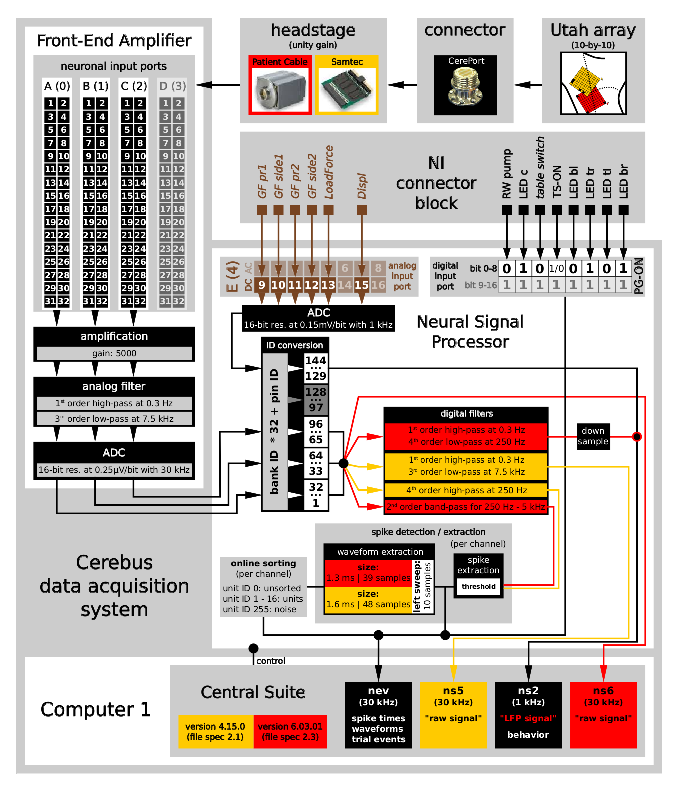
\includegraphics[width=0.7\textwidth]{./figures/scidata_figures/cerebus_system}
 \caption[Sketch of the components related to the recording of the neuronal signals]{Sketch of the components related to the recording of the neuronal signals. Data were recorded
using a Utah array, which was linked via its connector (CerePort) to a headstage (Samtec or Patient Cable) with a unity gain. From there the neural signals were transferred to the Cerebus Front-End Amplifier, where they were amplified, filtered and digitized. The digitized signals were converted into a single multiplex optical output and sent via a fiber-optic data link to the Neural Signal Processor (NSP), which is controlled by the Cerebus control software (Central Suite). Within the NSP the time points and waveforms of potential spikes were extracted online from a correspondingly processed copy of the neural signals and saved in the nev file. Simultaneously, the continuous raw signals (sampled at 30 kHz) were saved in the ns5 (for monkey L) or ns6 file (for monkey N). In parallel to the neural signals the NSP received also the digital trial events produced by the LabView VI, and the analog signals of the object’s sensors via the NI connector block of the behavioral control system. While the digital trial events were saved along with the extracted potential spikes in the nev file,
the analog signals of the sensors were digitized and saved in the ns2 file. For monkey N, a filtered and downsampled version of the neural signals (0.3–250 Hz at 1 kHz) was also saved in the ns2 file. Components and settings specific to monkey L and N are indicated by yellow and red, respectively.}
\label{fig:cerebus_system}
\end{figure}

A visual summary of the available data is given in \cref{fig:overview_data_l_1} and \cref{fig:overview_data_l_2}  for monkey L, and \cref{fig:overview_data_n_1} and \cref{fig:overview_data_n_2} for monkey N. The first of these figures shows the sequence of trials as well as selected raw recorded time series, spike trains, unit wave forms, and behavioral signals for one particular trial. The second of these figures contrasts parallel neuronal data across channels in a specific trial with neuronal data across trials in a specific channel.


\section{Data Preprocessing}
\label{sec:data_preprocessing}

After the recordings, a number of preprocessing steps (pre in the sense of before the actual upcoming data analysis, but being the post-processing after the recording) were performed as described below. This includes (i) the translation of the digital events from their binary codes set by the DAQ system to a human-readable format putting the events in context of the expected executed trial event sequence, (ii) the offline detection of behavioral trial events and object load force from the analog signals recorded by the sensors of the target object, and (iii) the offline spike sorting.

\subsection{Translation of digital events to trial events }

\cref{tab:bit_translation} lists the 8-bit combinations that were sent by LabView to the Experimental Apparatus to control the behavior. Following a binary to decimal conversion, they were saved as event codes (\cref{tab:bit_translation}) during the experiment along with their time stamps in the .nev file. In the first preprocessing step, these event codes were translated to a human-readable format and put into context of an expected trial event sequence. The validation against the latter was used to identify incomplete, correct and error trials. Error trials were further differentiated into error types (e.g., grip error). This digital event translation and interpretation (cf. \cref{tab:bit_translation}) performed automatically within the reach-to-grasp loading routine. 

Translation table of the 8 bits to the event codes and their behavioral meaning (labels). The 8 bits (see \cref{tab:bit_translation} for their meaning) were sent from LabView to NSP during the trial sequence (Fig. \cref{fig:task_trialscheme}). The event codes are the decimal version of the bit sequence assuming another byte with all bits set to 1 in front. The event codes are found in the .nev files with a time stamp and indicate the occurrence of a stimulus / behavioral event as indicated in the center colum ('label'). Due to different versions of the LabView control program for monkey L and N (see text for details) the event codes for the same label may be different for the two monkeys. Also some event codes do not have a concrete meaning (miscellaneous) and occur sporadically in the .nev file due to a mistake in the sampling of the digital events - they have to be ignored. In the table the event codes are sorted in sequential order from top to bottom with respect to the task, i.e. their order corresponds to the sequence found in the .nev file in an successful trial. 

\subsection{Preprocessing of behavioral analog signals}

Some behavioral events such as the monkey touching the object or the onset of the object displacement by the monkey were controlled during the experiment, but their online-detected timing was approximate and not saved (see details in section \cref{sec:behavioral_control_system}). However, these events can be relevant for data analysis and they were thus computed offline from the analog signals of the four FSR sensors measuring the monkey's grip and the HE sensor measuring the object displacement. We implemented a custom-made Matlab \code{Event}-Detection toolbox to detect 8 specific events: the precise timing of object touch (OT) and object release (OR) from the force traces as well as the timing of displacement onset (DO) and object back to baseline (OBB) from the displacement trace, and finally the onset and offset of the plateau phase in the force and displacement traces. The plateau phase of the displacement signal indicates the timing and stability of the holding period, and its onset is used to calculate offline the hold start (HS) signal. The toolbox performed an automatic detection of these events and their timing was first approximated by threshold crossing and then fine-tuned by back-comparison of the traces with baseline level from the point of threshold crossing. Since the automatic detection was prone to errors, the trials were visually inspected one by one and the timing of the automatically detected events were manually corrected if they did not match the event times as visually identified. In addition, a Matlab script was used to inspect the load force traces in each trial to control if the actual object load corresponded to the programmed object load. This procedure ensured that the electro-magnet controlling the object load was properly activated throughout the recording session. 

\subsection{Offline spike sorting}
\label{sec:offline_spike_sorting}
The spike waveforms which were extracted and saved (in the nev file) during the recording were offline sorted using the Plexon Offline Sorter (version 3.3.3). To keep the variability in the half-manual spike sorting at a minimum, all sortings were performed by the same person (A. Riehle). The spike sorting started with loading the complete nev file of a session into the Plexon Offline Sorter. The spike sorting was performed on a duplicate of the data file to keep the original data intact. We started by joining all different waveforms extracted online from each channel separately back again into one pool and initially marked as “unsorted waveforms” in the Plexon Offline Sorter. Thereby, we ignored the result of the preliminary online waveform sorting (units 0-16 in the nev file) that was performed during the recording via Central Suite software, which served solely to extract waveforms and gain an overview of the quality of the spiking activity. For the invalidation of cross-channel artifacts (e.g., chewing artifacts) all waveforms that occurred simultaneously on a defined percentage of channels (70\%) were marked as “invalidated waveforms” in Plexon Offline Sorter. Such artifacts occurred only in the recording session of monkey L. Furthermore, a waveform rejection was performed. Thereby all waveforms of abnormally large amplitude and/or atypical shape on a channel were manually marked as “invalidated waveforms” in Plexon Offline Sorter.

The actual spike sorting was then performed on the remaining unsorted waveforms (i.e., those not marked as invalidated waveforms) individually for each channel. We used different algorithms to split these waveforms into clusters in a 2- or 3-dimensional principal component (PC) space. The dimensionality of the PC space was chosen according to the best separation. The main algorithms used were K-Means(-Scan) and Valley Seeking (chosen according to the best separation). We used a fixed threshold for outliers (a parameter to be determined in the Plexon Offline Sorter) between 1.8 (K-Means) and 2 (Valley Seeking) to get comparable sorting results. The spikes of the sorted clusters were then controlled using the inter-spike interval (ISI) distributions and the auto- and cross-correlation plots. Units were ordered manually from best to worst (assigning increasing unit IDs 1-16 in the Plexon Offline Sorter) by considering the amplitude of the waveform (the higher the better), the outcomes of the ISI analysis (no or low number of spikes with an ISI smaller than 2 ms), the correlation histograms, and identifiable cluster shapes. Waveforms in the cluster with the highest unit ID (worst) on a given channel may contain multi-unit activity. Clusters with unacceptable outcomes (completely or partly overlapping waveforms), including those with only a few spikes, left assigned as “unsorted waveforms” in Plexon Offline Sorter. This offline spike sorted nev file was saved under the file name of the original nev file with an added two-digit numeric postfix (e.g. -01). In this file, unit ID 255 contains invalidated waveforms, unit ID 0 contains the unsorted waveforms (that may enter a further cluster analysis for spike sorting), and unit IDs 1-16 contain the time stamps and waveforms of the sorted single- or multi-units (as in the Plexon Offline Sorter). Unit IDs that are considered to represent multi-unit activity are documented in the metadata. The nev file with the sorted units can be loaded again into the Plexon Offline Sorter to visualize all the sorted spikes and rework the spike sorting.

\begin{table}
\centering
\begin{tabular}{cccccc}
\hline 
\multirow{2}{*}{\textbf{monkey}} & \multirow{2}{*}{\textbf{sorting ID}} & \multirow{2}{*}{\textbf{\# SUA}} & \multirow{2}{*}{\textbf{\# MUA}} & \multicolumn{2}{c}{\textbf{\# electrodes with}}\tabularnewline
% \cline{5-6} 
 &  &  &  & \textbf{SUA} & \textbf{SUA or MUA}\tabularnewline
\hline 
\hline 
\textbf{L} & {*}-02 & 93 & 49 & 65 & 86\tabularnewline
\textbf{N} & {*}-03 & 156 & 19 & 78 & 89\tabularnewline
\hline 
\end{tabular}

\caption[Overview of offline sorted single and multi unit activity (SUA and MUA)]{Overview of offline sorted single and multi unit activity (SUA and MUA). For the recording of monkey L it was possible to sort out 93 SUAs and 28 MUAs distributed over 65 of the 96 electrodes of the Utah array, with 21 additional electrodes with further MUA recordings. For the recording of monkey N it was possible to sort out 156 SUAs and 8 MUAs distributed over 78 of the
96 electrodes of the Utah array, with 11 additional electrodes with further MUA recordings. For details on the offline spike sorting see \cref{sec:offline_spike_sorting}.}
\label{tab:datafiles_unitactivity}
\end{table}

\subsection{Code availability}
\label{sec:code_availability}

All available code required to access the data as described in \cref{sec:usage} is stored along with the datasets. The provided code includes, in particular: (i) a snapshot of the Python \software{Neo}  package (see also \cref{sec:neo}), (ii) a snapshot of the Python \software{odML} package (see also \cref{sec:odml}), (iii) the custom-written ReachGraspIO extending the \software{Neo} package, (iv) the example script shown and described in \cref{sec:usage}, (v) the code shown and described in \cref{sec:usage} demonstrating how to access the data in \software{Matlab}.

In addition to these frozen versions of the code, we recommend to use updated versions of the code to benefit from future enhancements, bug fixes and increased compatibility with future Python releases or novel applications that rely on recent versions of \software{Neo} and/or \software{odML}. Complete link collections to the two libraries can be found online\footnote{\software{Neo}, \url{http://neuralensemble.org/neo/}},\footnote{\software{odML}, \url{ and http://www.g-node.org/projects/odml}}. Importantly, both projects are hosted and version-controlled via Github\footnote{\software{Neo}, \url{https://github.com/NeuralEnsemble/python-neo}},\footnote{\software{odML}, \url{https://github.com/G-Node/python-odml}}.

\section{Data Records}

All data and metadata are publicly available via the data portal of the German Neuroinformatics Node (G-Node) of the International Neuroinformatics Coordination Facility (INCF), called GNData\footnote{GNData, \url{http://g-node.github.io/g-node-portal/}}. \cref{tab:scidata_data_overview} provides an overview of the name, size, and content of all files for each published dataset of monkey L and N. The datasets of both monkeys consist of four parts: (i) the primary data are provided as the original data files obtained from the Central Suite software stored in the data format specified by the manufacturer (in particular, nev, ns5 and ns6 format) of the neural recording platform, Blackrock Microsystems; (ii) an offline sorted version of the neural spike data (cf. \cref{sec:offline_spike_sorting}) is provided in a second nev file; (iii) metadata are provided as one file per dataset in the \software{odML} format \citep{Grewe_2011, Zehl_2016}; and (iv) a mat file is provided containing the continuous neural raw data together with the offline sorted spike data, both annotated with the corresponding metadata.

\begin{figure}
 \centering
 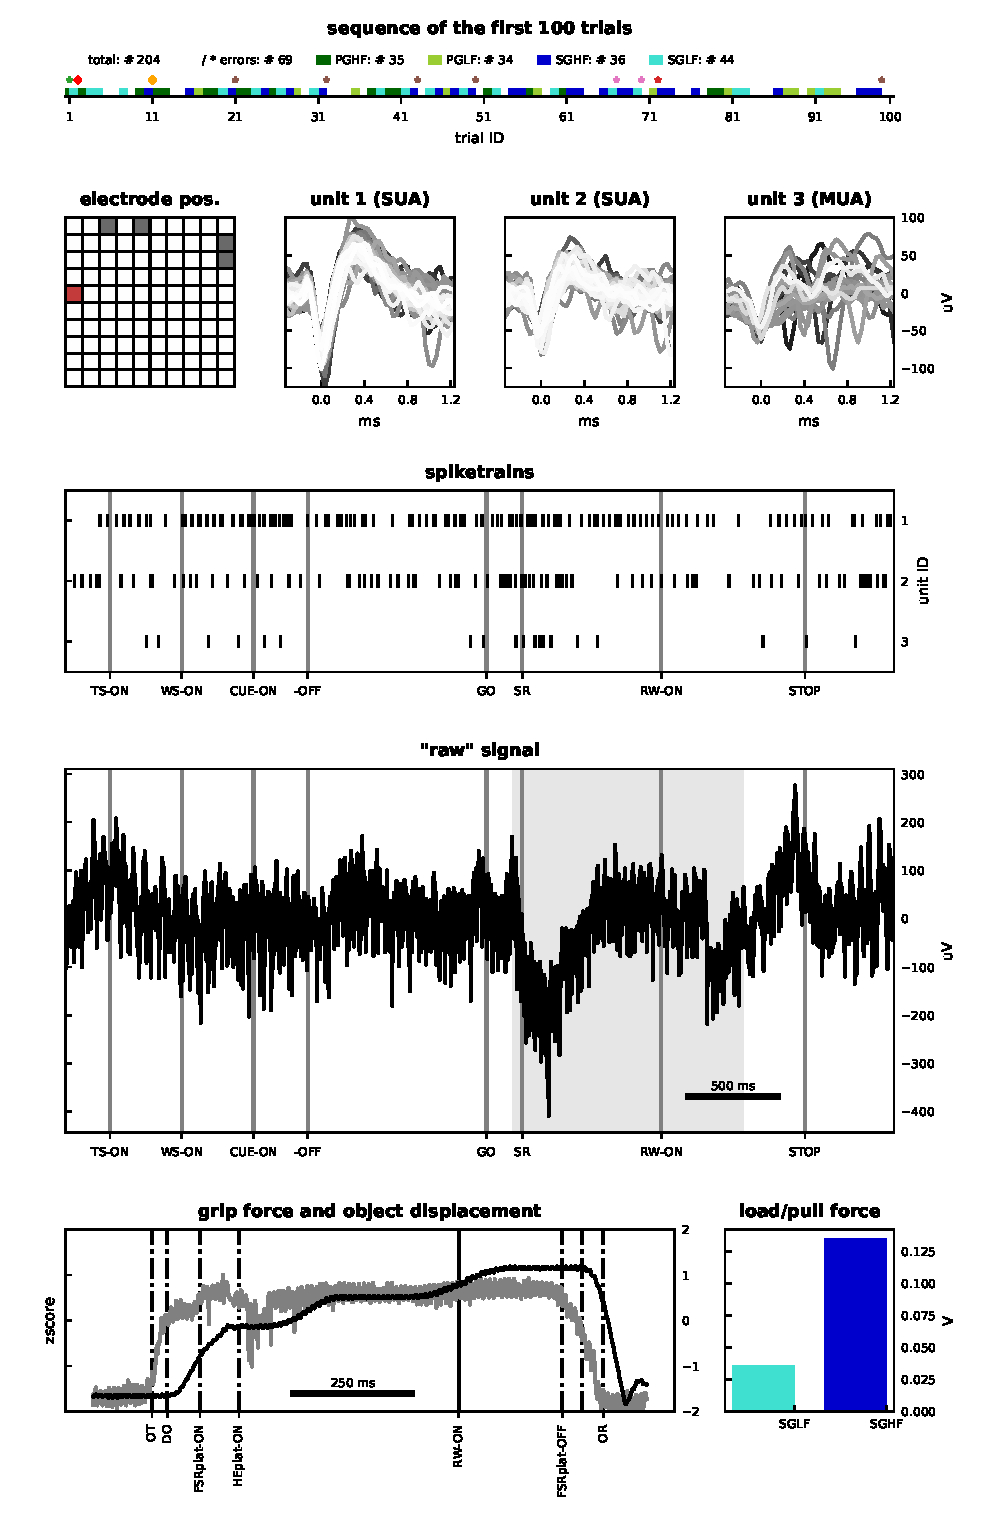
\includegraphics[width=0.8\textwidth]{./figures/scidata_figures/data_overview_1_L}
 \caption[Overview of data types contained in l101210-001]{Overview of data types contained in l101210-001. The figure displays the different data types contained in the selected dataset of monkey L. Top panel: sequence of the first 100 trials (for trial types and errors see color in legend) and the total number of trials (see \# for correct, error, trial types in legend); the red diamond marks the selected trial (trial ID: 2) for panels below; the orange diamond marks an additional trial selected to demonstrate load/pull force differences between the averaged load force signals in the bottom right panel. Asterisks indicate error trials (black asterisks: grip errors). Second row, left panel: position of selected electrode (in red) for the data plots (electrode ID: 71). Second row, remaining panels: waveforms of three units from the selected electrode. Third row: spike trains of displayed units for the selected trial. Forth row: raw signal for the selected trial; gray shaded area marks the time window corresponding to the bottom left panel. Bottom left panel: grip force (gray) and object displacement (black) signals for the selected trial. Bottom right panel: averaged load/pull force signals for the duration of the plateau of the grip force signal for the selected LF and HF trial. Important trial events are indicated as vertical lines in the corresponding data plots.}
 \label{fig:overview_data_l_1}
\end{figure}

\begin{figure}
 \centering
 \includegraphics[width=\textwidth]{./figures/scidata_figures/data_overview_2_L}
 \caption[Overview of raw signal and spike data of monkey L (l101210-001)]{Overview of raw signal and spike data of monkey L (l101210-001). Left panels: Raw signal (top) and spike data of unit IDs 1 on each given electrode (bottom) for a single trial (trial ID: 2) across a selection of electrodes. Right panels: Raw signal (top) and spike data from single unit ID 1 (bottom) across selected correctly performed trials on one electrode (electrode ID: 3). Trial events (TS-ON, WS-ON, CUE-ON, CUE-OFF, GO-ON, and RW-ON) are indicated as colored vertical lines in each plot. Trial types of selected trials in upper right panels are indicated as color (SGHF: dark blue; SGLF: cyan; PGHF: dark green; PGLF: light green)}
 \label{fig:overview_data_l_2}
\end{figure}

\begin{figure}
 \centering
 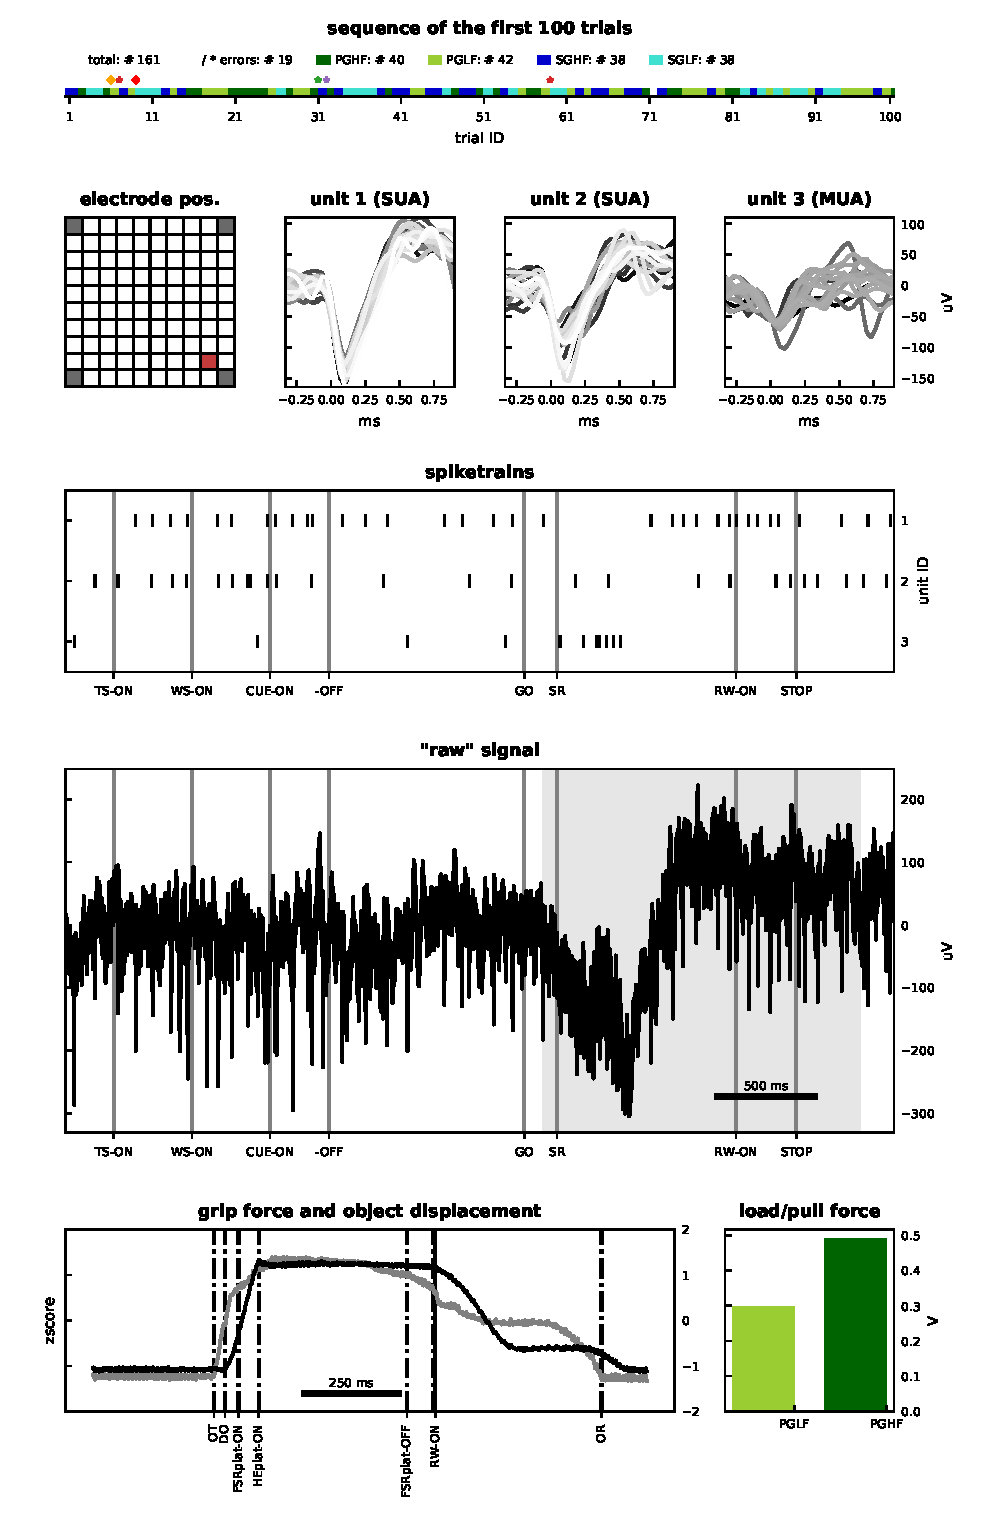
\includegraphics[width=0.8\textwidth]{./figures/scidata_figures/data_overview_1_N}
 \caption[Overview of data types contained in i140703-001]{Overview of data types contained in i140703-001. The figure displays the different data types contained in the selected dataset of monkey N. Top panel: sequence of the first 100 trials (for trial types and errors see color in legend) and the total number of trials (see \# for correct, error, trial types in legend); the red diamond marks the selected trial (trial ID: 9) for panels below; the orange diamond marks an additional trial selected to demonstrate load/pull force differences between the averaged load force signals in the bottom right panel. Asterisks indicate error trials (black asterisks: grip errors). Second row, left panel: position of selected electrode (in red) for the data plots (electrode ID: 63). Second row, remaining panels: waveforms of three units from the selected electrode. Third row: spike trains of displayed units for the selected trial. Forth row panel: raw signal for the selected trial; gray shaded area marks the time window corresponding to the bottom left panel. Bottom left panel: grip force (gray) and object displacement (black) signals for the selected trial. Bottom right panel: averaged load/pull force signals for the duration of the plateau of the grip force signal for the selected LF and HF trial. Important trial events are indicated as vertical lines in the corresponding data plots.}
 \label{fig:overview_data_n_1}
\end{figure}

\begin{figure}
 \centering
 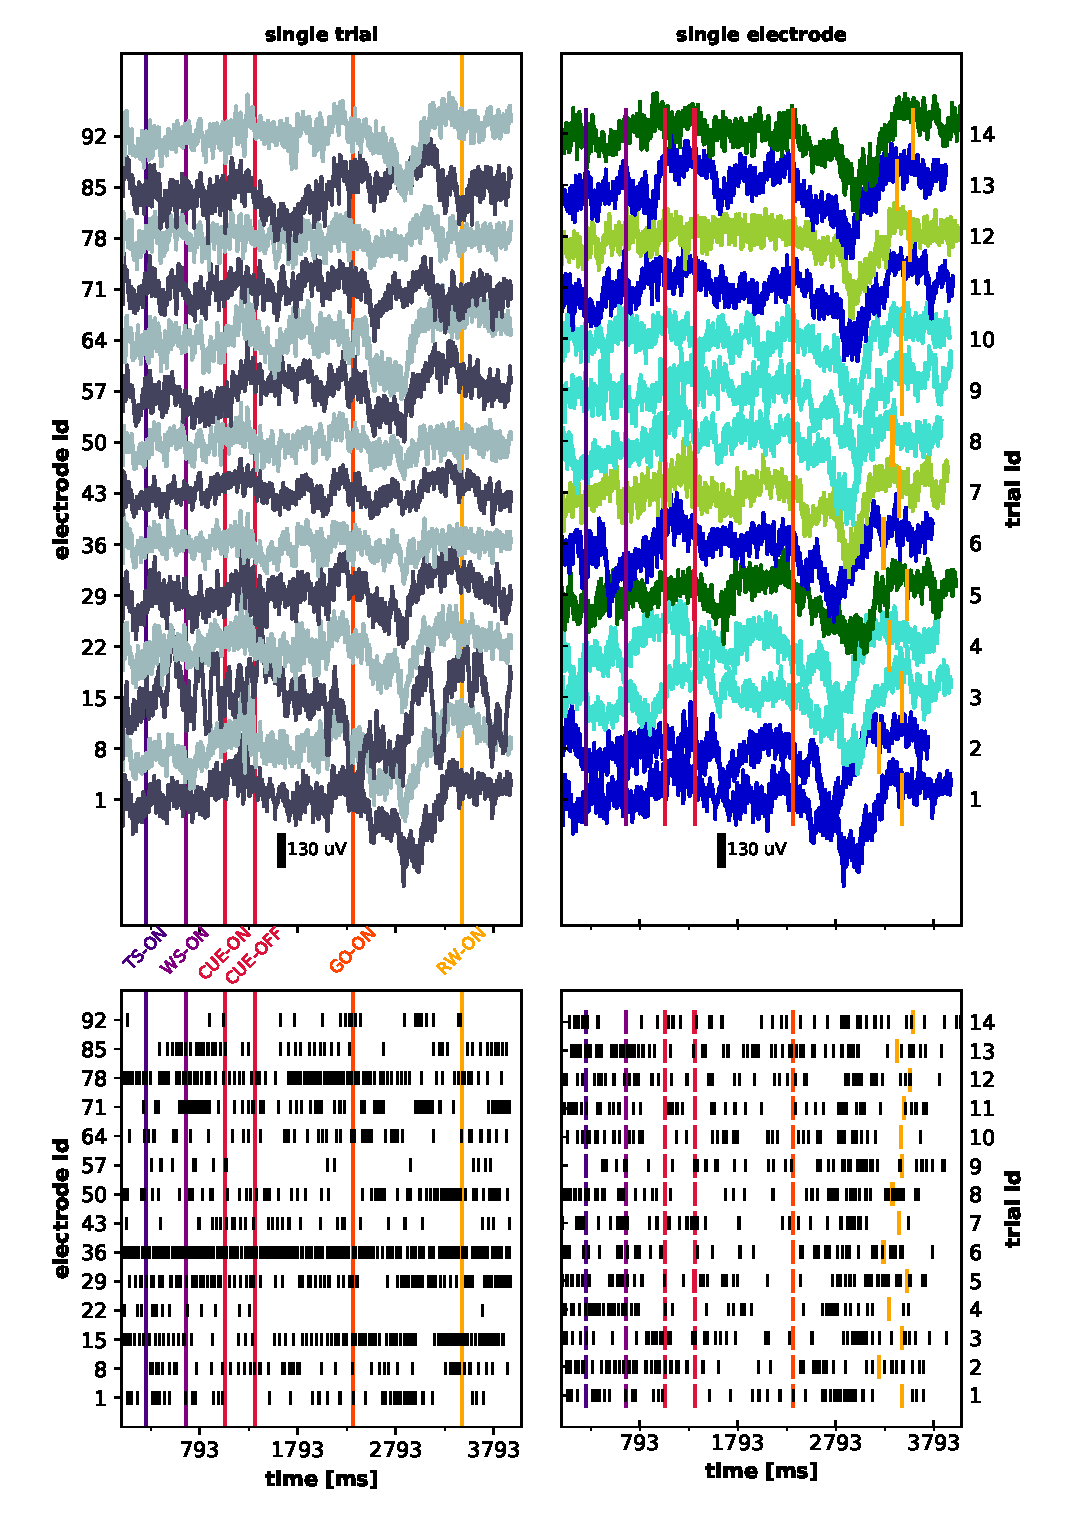
\includegraphics[width=\textwidth]{./figures/scidata_figures/data_overview_2_N}
 \caption[Overview of LFP and spike data of monkey N (i140703-001)]{Overview of LFP and spike data of monkey N (i140703-001). Left panels: LFP data (top) and spike data of unit IDs 1 on each given electrode (bottom) for a single trial (trial ID: 1) across a selection of electrodes. Right panels: LFP data (top) and spike data from single unit ID 1 (bottom) across selected correctly performed trials on one electrode (electrode ID: 1). Trial events (TS-ON, WS-ON,CUE-ON, CUE-OFF, GO-ON, and RW-ON) are indicated as colored vertical lines in each plot. Trial types of selected trials in upper right panels are indicated as color (SGHF: dark blue; SGLF: cyan; PGHF: dark green; PGLF: light green).}
 \label{fig:overview_data_n_2}
\end{figure}


Overview of recording days of the published datasets. For both monkeys, we chose to publish the first dataset (rec*-001) of the recording day. For details on the published datasets see \cref{tab:scidata_data_overview}.

The dataset l101210-001 from monkey L is the first out of 9 recording sessions conducted on Friday, December 10, 2010, while the dataset i140703-001 from monkey N is the first out of only 3 recording sessions conducted on Thursday, July 3, 2014. Both datasets were recorded in the late morning. The following recording day went on for nearly one hour and a half for monkey L, and one hour for monkey N. Although the recording from monkey N lasted with 16:43 min several minutes longer than the recording from monkey L with only 11:49 min, monkey L executed 204 trials, while monkey N only performed 160 trials in total. However, monkey L performed only ~70\% of all trials correctly, whereas monkey N successfully completed ~90\% of all trials during the recording (cf. \cref{tab:scidata_data_overview}). Nonetheless, the high percentage of error trials in monkey L are mainly caused by an too early movement onsets reflecting the eagerness, but also the nervousness of the monkey L's character. In contrast to these error types, monkey L used only 12 times the wrong grip compared to monkey N who performed an incorrect grip type 16 times during the recording. 

Overview of trials performed during the published datasets. Of the stated number of error trials, the monkey L and N used the wrong grip type in 12 and 16 trials, respectively. In the remaining error trials the monkeys initiated the movement too early. Trial types were altered randomly in the recordings which led to slightly different trial numbers for the different trial types.

For both monkeys the trial types alternated randomly between trials leading to slightly different numbers of trials with the same trial type in the each dataset (cf. \cref{tab:scidata_data_overview}). 

The quality of the spiking activity in the datasets of both monkeys was high, which allowed us to perform a relatively robust offline spike sorting with high numbers of single unit activity (SUA) distributed over all electrodes of the array (for details see \cref{tab:datafiles_unitactivity}). For details on how the offline sorting was performed and checked please have a look at \cref{sec:offline_spike_sorting} and \cref{sec:spike_data_quality}. 


\section{Technical Validation}
\label{sec:technical_validation}

In addition to the above described preprocessing steps that needed to be performed to gain more content of the raw data, some technical validations of the data also had to be conducted. These technical validations include the correction of the irregular alignment data files of the Cerebus DAQ system and a general quality assessment of the data. In order to validate the quality of the recording, a series of algorithms were applied to the data. On the one hand the quality of the LFP signals was assessed per electrode and per trial by evaluating the variance of the corresponding signal in multiple frequency bands. On the other hand the quality of the offline sorted single units (\cref{sec:offline_spike_sorting}) was determined by a signal-to-noise measure. In addition, noise artifacts occurring simultaneously in the recorded spiking activity were detected and marked. In the following, we explain these technical validation steps in detail.

\subsection{Correction of data alignment}

The ns6 file starts always 82 samples later than ns5, ns2 and nev files. This miss-alignment is caused by an error in the Blackrock recording software. However, this shift is correctly recorded in the ns6 file, and therefore will be automatically corrected in the generic \software{Neo} loading routine (cf., BlackrockIO in \cref{sec:usage} below). In addition, due to the online filter procedure, the LFP signals in the ns2 file are delayed by approximately 3.6 ms with respect to the time stamps in the nev file and the analog signal of the ns6 file. This offset was heuristically determined, documented in the metadata file, and can be automatically corrected for by the experiment-specific loading routine (cf., ReachGraspIO in \cref{sec:usage} below). Note that the time stamps of the spike times provided in the nev file correspond to start of the waveform and not to the time point of threshold crossing.

\subsection{Quality assessment}

The occurrence of noise in electrophysiological recordings is to a certain degree unavoidable and therefore needs to be carefully examined. It depends to a large extent on the quality of the headstage used to record the neurophysiological data. In our data, two different types of headstages were used for the two monkeys - the Samtec-CerePort headstage (monkey L) and the Patient Cable (monkey N). The former is much more sensitive to noise than the latter. The type of noise, its cause and appearance in the data is quite variable. Depending on the direct influence of the different types of noise on subsequent analysis methods, one needs to balance the corresponding data rejection between being very permissive and very conservative. For this reason, it is wise not remove or delete data of bad quality, but instead mark them with the judgment of a corresponding quality assessment procedure. For the here published datasets, we provide the results of our quality assessment of the electrodes, trials and spiking units along with the analysis parameters of the used procedure in the \software{odML} metadata files for each recording. The reach-to-grasp IO integrates this information by annotating the corresponding data objects in Neo. This approach not only allows the user to finally decide which data to reject for an analysis, but also provides the opportunity to provide different quality assessments of the same electrode, trial and unit at the same time. This is helpful if one considers that certain types of noise can differently contaminate signals in different frequency bands. For the here published datasets, the quality of the recorded signals was therefore separately tested for the sorted spike data and different frequency bands of the LFP data. The used corresponding procedures are described in detail below. 

\subsection{LFP data quality}

The LFP data were examined for noise in three broad frequency bands excluding the 50Hz European line noise (low: 3Hz - 10Hz, middle: 12Hz - 40Hz, high: 60Hz - 250Hz) in each session individually. The goal of the quality assessment was, first, to detect channels with a noisy signal throughout the session and, second, to detect noisy trials in the remaining “clean” channels. To do so, the analog signals of each electrode were first z-scored and filtered in the three frequency bands (low, middle, and high) using a Butterworth filter (of order 2, 3, and 4, respectively). For each frequency band the quality assessment analysis was carried out separately. The detection of noisy electrodes was performed in three steps: 

step 1 The variance of the filtered analog signal of each electrode was calculated over the complete session. 

step 2 Out of the 96 resulting variance values, outliers were identified as those values outside a user-defined range. The range was defined as follows: (i) values between a lower (e.g., 25th) and an upper (e.g., 75th) percentile (L and U), (ii) the range of acceptable values was defined by $L-w\cdot(U-L),U+w\cdot(U-L)$,where w is a user-defined whisker coefficient (e.g., w=3). 

step 3 The analog signals classified as outliers in step 2 were visually controlled by comparing them to the analog signal of an electrode with a typical variance value. If the results were either too conservative or too permissive, the detection procedure was repeated by manually adapting the chosen parameters (L, U, and w), correspondingly. 

The electrode IDs of the final outliers as well as the parameters chosen for their detection were saved in the \software{odML} metadata file of the corresponding recording and marked as noisy for the tested frequency band. 

For the remaining non-noisy electrodes, an analogous procedure was carried out afterwards to detect noisy trials. The procedure differed in one respect: the variance of the filtered analog signal was calculated for each trial on each electrode separately. At the end, the trial IDs of the identified outliers were pooled and marked as noisy for the tested frequency band on all electrodes. The marked trial IDs were saved in the \software{odML} metadata file of the corresponding recording together with the chosen analysis parameters for their detection. Note again that with this procedure a trial is marked as noisy on all electrodes as soon as it is classified as noisy on one electrode.

\subsection{Spike data quality}
\label{sec:spike_data_quality}

To test and judge the quality of the spike data, the results of the offline spike sorting were controlled first, for the signal-to-noise ratio (SNR) from the waveforms of the identified single units and second, for the occurrence of hyper-synchronous event artifacts.

1. To calculate the SNR for each identified unit in the sorting results a method introduced by \citet{Hatsopoulos_2004} was used. The SNR was defined as the amplitude (A, trough-to-peak) of the mean waveform ($<w>$) divided by twice the standard deviation of the waveform noise ($SD_{noise}$) of the defined unit (u): $SNR_{u}=A_{<w>}/SD_{noise}\cdot2$,where $SD_{noise}$ was computed by averaging the standard deviations (SDs) obtained from each sample point across the original waveforms (SD of the waveform noise adapted from \citet{Nordhausen_1996,  Suner_2005}. For all identified single units in the datasets published here, the determined SNRs ranged between $1.5$ and $12$. Corresponding to \citet{Suner_2005} the quality of the spike sorting of an identified unit is good if the SNR is above 4, is fair if the SNR ranges between 2 and 4, and is poor if the SNR ranges between 1 and 2. Units with an SNR below 1 are not considered as signals. For a conservative analysis of the spike datasets, we recommend to use only single units with a SNR of 2.5 or higher, which was our choice in e.g. \citet{Torre_2016}. The results of the SNR analysis of the performed spike sorting were saved in the \software{odML} metadata file of the corresponding recording and units were annotated accordingly. 

2. Since correlation analysis of spike data is very sensitive to cross-electrode artifacts which would produce unwanted false positive results, we controlled the sorted spike data on their original time resolution ($\delta=1/30ms$) for potential occurrence of hyper-synchronous event artifacts. For this, we computed the population histogram, i.e. the sum of the spikes across all sorted single units in the dataset in bins of $\delta=1/30ms$ (sampling resolution of the data), and detected if there were entries $\ge2$. To our surprise these hyper-synchronous spikes, which are likely to be attributed to cross-channel noise, survived the spike sorting including the cross-channel artifact removal by the Plexon Spike sorter. We indeed detected these spike artifacts during a preliminary analysis of a previous study \citep{Torre_2016}. The number of single units participating in these events ranged from 2 to over 30 and a statistical analysis showed that the frequency of their occurrence largely exceeded the expected value considering the observed population firing rate. Furthermore, a $\delta$-binned time histogram of the population spiking activity triggered around the occurrence times of the hyper-synchronous events revealed also increased spiking activity in the preceding or following bin of the event. For a conservative analysis of the spike datasets, we recommend to treat the spikes participating in a hyper-synchronous event as well as the spikes occurring within a short time interval around this event ($\scriptstyle \pm\delta$) as artifacts of unknown origin and to remove them subsequently before performing any analysis of the spike data.

In \citet{Torre_2016} we combined both quality assessments of the spike data and only considered spikes with a SNR>2.5 and additionally removed all hyper-synchronous events with $\ge2$ spikes. 


\section{Usage Notes}
\label{sec:usage}

In the following, we describe how the provided data files can be practically used in a data analysis scenario. To this end, we first briefly present the open source software libraries we recommend to use in order to access data and metadata using the Python programming language. We also demonstrate how to merge data and metadata in a common representation that facilitates data handling and analysis. Finally, we present an example program that produces a visualization of the most important data items contained in the files, and can be used as a template script for accessing the provided data. All software discussed below is provided in the code subfolder of the provided datasets, and links to the code repositories are listed in \cref{sec:code_availability}.

As outlined above, the datasets are stored in two types of files. The primary data, and the spike sorted data, are provided in the data format (in particular, the nev, ns5 and ns6 format) specified by Blackrock Microsystems, the manufacturer of the recording hardware. Second, metadata are provided as one file in the \software{odML} format \citep{Grewe_2011}. While data and metadata are provided in documented file formats (see Blackrock\footnote{Blackrock, \url{http://blackrockmicro.com/}} and \software{odML}\footnote{\url{http://www.g-node.org/projects/odml}}, respectively), the mere knowledge of the highly complex internal structure of the files is insufficient to practically make use of their content. In particular, implementations of corresponding loading routines performed from scratch by individual researchers are likely to be incoherent and error-prone. Thus, in the following we will use two community supported open-source libraries to separately load primary data and metadata into a generic, well-defined data representation. 

We chose the data object model provided by the open-source \software{Neo} library (\cref{sec:neo}) \citep{Garcia_2014} as the primary representation of the datasets (\cref{sec:neo}). \software{Neo} provides a hierarchical data structure composed of Python objects that aim to represent electrophysiological data in a generic manner. In addition, \software{Neo} provides a number I/Os that enable the user to read from (and in part, write to) a large number of open and vendor-specific file formats. In particular, \software{Neo} provides an I/O module for the file format used by Blackrock Microsystems (class BlackrockIO in file neo.io.blackrockio.py). The output of this I/O is a \software{Neo} data structure that is a faithful representation of the contents of the primary data files. For detailed information on the structure of the \software{Neo} data object model, please consult the online documentation\footnote{Neo, \url{http://neo.readthedocs.io/en/latest/index.html}}.

Here, we briefly summarize the output of the reach-to-grasp datasets obtained when calling the I/O. The \code{read\_block} method of an instantiation of the BlackrockIO returns a \software{Neo} Block object as a top level grouping object representing one recording session. In the hierarchy directly below the Block is one single \code{Segment} object spanning the complete continuous recording, and one \code{ChannelIndex} object for each of the 96 electrodes of the Utah Array (\cref{fig:implant_locations}) and each of the 6 sensor signals monitoring the target object manipulation (\cref{sec:experimental_apparatus}). The data from these 102 recording channels is each saved in one \code{AnalogSignal} object. All of these are linked to the \code{Segment} and the respective \code{ChannelIndex} object. Likewise, the spike times (and optionally, the spike waveforms) of each identified unit are saved to a \code{SpikeTrain} object. As for the \code{AnalogSignal} objects, these are linked to the \code{Segment}, and to the \code{ChannelIndex} object via a Unit object. Finally, all digital events are saved into a single \code{Event} object that lists their time of occurrences and the corresponding event IDs. Additional information from the file is provided as annotations on each individual \software{Neo} object (accessible via the annotation property of the object), in particular as annotations to the top level Block object. Note, that although this generic I/O can be used to access the raw data records, no interpretation of the file contents is given. For example, digital events are not interpreted as behavioral events, but only given as the raw numeric codes shown in \cref{fig:scidata_setup_overview}. 

In order to access the metadata stored in the \software{odML} file, we use the corresponding library API python-\software{odML} described in \citet{Grewe_2011}. In short, \software{odML} files store metadata in form of hierarchically structured key-value pairs. The \software{odML} files accompanying the provided datasets contain extensive metadata grouped into different sections describing different aspects of the experiment. A tutorial on how to work with the \software{odML} library can be found in the online documentation shipped with the library, and a more detailed description of how to manage metadata by example of the \software{odML} framework can be found in \citet{Zehl_2016}. In short, the library supports to read the content of an \software{odML} file, provides an API to navigate through the hierarchical structure, and to extract metadata of interest from the key-value pairs. Thus, the python-\software{odML} library provides a standardized way to access stored metadata records. 

As a next step, we combine the primary data and metadata in a manner that is specific to this experiment and aids the analysis process. To this end, the relevant metadata that were extracted from the \software{odML} are attached as annotations to data objects in the hierarchical \software{Neo} structure. For example, metadata information for a particular single unit originating from the spike sorting process may be attached to the \software{Neo} objects representing the sorted spike data of that unit. The task of combining the primary data and metadata is performed by a custom-written Python class named ReachGraspIO that is derived as child class from Neo's BlackrockIO class. For a full documentation of the input arguments, methods, and outputs of this class, please refer to the class documentation in reachgraspio.py. In short, invoking the \code{read\_block} method of the ReachGraspIO performs the following steps under the hood: (i) read the primary data using the \code{read\_block} method of the parent class (BlackrockIO) as described above, (ii) read the metadata using the python-\software{odML} library, (iii) interpret event data based on the digital events (e.g., detect trial start or reward), and (iv) add relevant metadata to the \software{Neo} data object using the annotation mechanism. Thus, the \software{Neo} Block object returned by the ReachGraspIO contains extensive information attached as annotations of the individual \software{Neo} objects, in particular, about whether a \code{SpikeTrain} is classified as SUA or MUA, about the spatial positioning of electrodes, or about the identities of electrodes that should be rejected. A full list of these metadata annotations can be found in the documentation of the \code{read\_block} method in the file reachgraspio.py.

In summary, for practical purposes, the resulting data structure of the ReachGraspIO hosts a complete representation of the data and a synthesis of the metadata relevant for analysis. This representation may be saved to disk in a standardized container format (e.g., .mat or HDF5), such that the exact same data and metadata context can also be accessed from other programming languages. For illustration, we provide the data object in the Matlab file format (.mat) in the folder datasets\_matlab, containing Matlab structs resembling the Python \software{Neo} objects.

In the following we demonstrate how to use the ReachGraspIO in practice in order to load and visualize the datasets. We follow the file example.py, which is contained as part of the code included with the published datasets. The goal of this program is to create a figure showing the raw signal, LFP, spikes (time stamps and waveforms), and events in a time window (referred to as analysis epoch) around TS-ON of trial 1 for electrode ID 62. 

In a first step, we load the data using the ReachGraspIO. Considering that only for monkey N an online filtered version of the LFP data is available in the ns2 file, in the following we calculate offline an LFP signal from all raw signals contained in the ns5 or ns6 files using a non-causal low-pass Butterworth filter implemented in the Electrophysiology Analysis Toolkit (Elephant\footnote{Elephant, \url{http://neuralensemble.org/elephant/}}, which provides analysis capabilities for data stored in the \software{Neo} representation. The parameters of this filter are chosen identical to those of the causal filter for the LFP recorded online in monkey N (\cref{sec:neural_recording_platform}).

In a subsequent step, we extract all TS-ON events in correctly performed trials. To this end, we use the function get\_events() contained in the utility module neo\_utils.py. The function extracts a list of events contained in one \code{Event} object of the loaded \software{Neo} \code{Block} given the filter criteria specified by the parameter event\_prop. In our example, the used filter criteria select all events from the \code{Event} object “TrialEvents” with a trial\_event\_labels annotation set to TS-ON, and a performance\_in\_trial annotation indicating a correct trial.

In a next step, we create \code{Epoch} objects representing analysis epochs around the extracted TS-ON events. To this end, we use add\_epochs() also contained in the utility module neo\_utils.py. The function excepts the previously extracted TS-ON events as trigger, and defines epochs of a given duration around this trigger. The resulting \code{Epoch} object is called “analysis\_epochs”. 

Next, we cut the data according to the analysis epochs and align the cutouts in time. This operation is performed by cut\_segment\_by\_epoch, which returns a list of \code{Segment} objects, each containing data of one analysis epoch. The \code{Segment}s are annotated by the corresponding annotations of the \software{Neo} \code{Epoch}. In addition, the list of \code{Segment} objects is grouped in a new \software{Neo} \code{Block}, named “data\_cut\_to\_analysis\_epochs”. This representation now enables the analysis of the data across trials in the defined analysis epochs. 

In our example, we show how to create a plot of the data of the analysis epoch in one behavioral trial on the selected electrode. To select the \software{Neo} \code{Segment} corresponding to the first correct behavioral trial from the \code{Block} of the cut data obtained in the previous step, we apply the \software{Neo} filter() function. 

From the selected \code{Segment}, LFP data and raw signals can be obtained via the \code{AnalogSignal} objects referenced by the analogsignals property, while spike trains and corresponding unit waveforms can be extracted from the \code{SpikeTrain} objects referenced by the spike trains property. The remainder of example.py uses the matplotlib library to create a figure of the data.

All data and metadata files as well as the code described above can be found in the data repository at GIN\footnote{GIN, \url{https://web.gin.g-node.org/INT/multielectrode_grasp}}. The subdirectory datasets contains all data files and the metadata odML-file for the two provided recording sessions. The subdirectory code contains the files example.py and neo\_utils.py. For further reference and inspiration this subdirectory also contains the Python scripts generating the data figures of this manuscript. Furthermore, the subdirectories to code contain frozen versions of the required libraries (\software{Neo}, \software{odML}) as well as the custom loading routine combining data and metadata (reachgraspio.py). Finally, the datasets\_matlab directory contains the annotated \software{Neo} data object containing all primary data saved in the mat-file format.







%%%%%%%%%%%%%%%%%%%%%%%%%%%%%%%%%%%%%%%%%%%%%%%%%%%%%%%%%%%%%
%BIBLIOGRAPHY
%%%%%%%%%%%%%%%%%%%%%%%%%%%%%%%%%%%%%%%%%%%%%%%%%%%%%%%%%%%%%

\clearpage
\renewcommand*{\thesection}{}\textbf{}

\printbibliography
% \bibliography{lesson7a1} 
% \bibliographystyle{ieeetr}
% \bibliographystyle{apacite}
% \bibliography{thesis}


\end{document}
